%!TEX root = ../csuthesis_main.tex
% 论文正文是主体,主体部分应从另页右页开始,每一章应另起页。一般由序号标题、文字叙述、图、表格和公式等五个部分构成。
\section{绪论}
\subsection{研究背景与意义}

\subsection{国内外研究现状}

\subsection{主要研究内容}

\subsection{论文组织结构}

\begin{figure}[hbt]
	\centering
	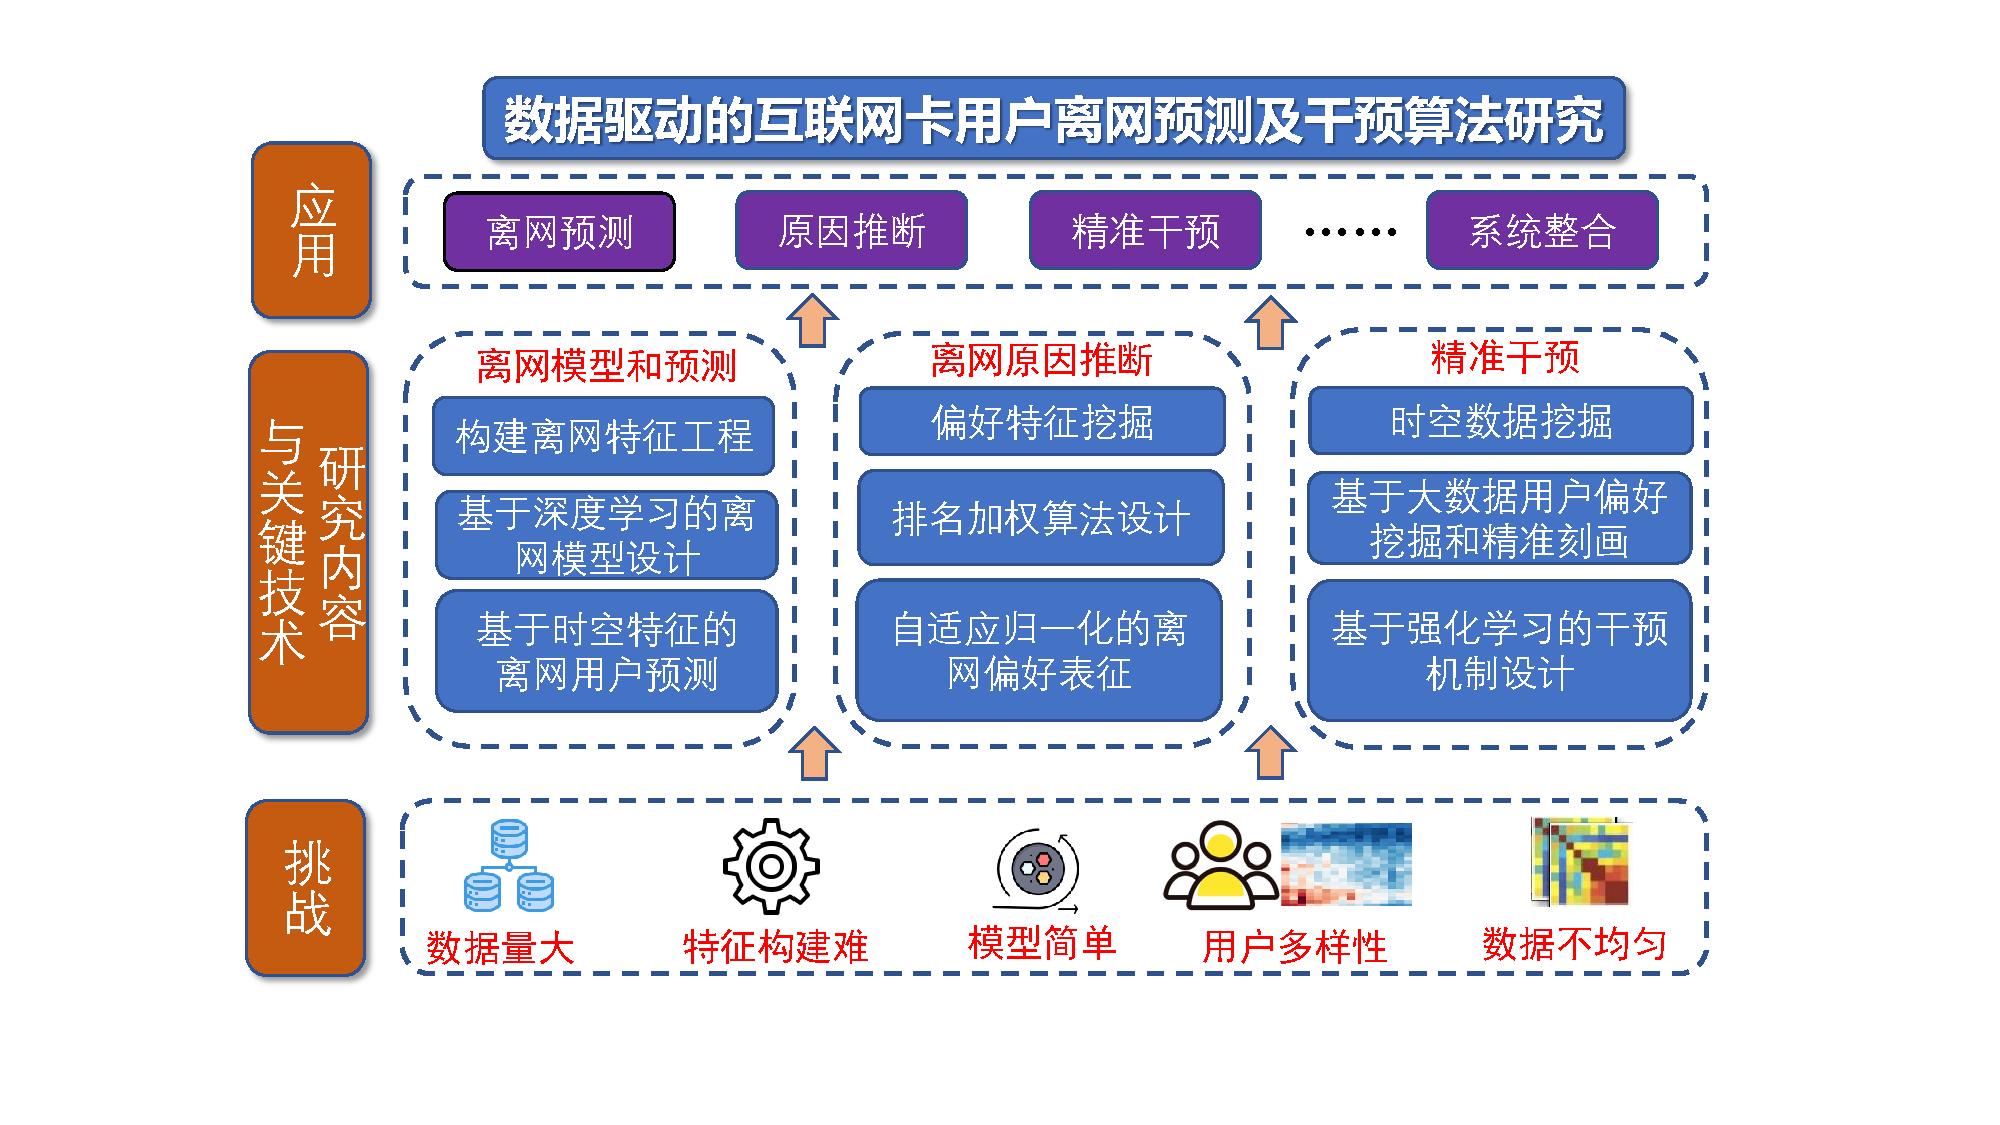
\includegraphics[width=1\textwidth]{Ms-start_Paper-Architecture_v1_1.pdf}
	\caption{论文组织架构图}
	\label{Fig:Paper-Architecture}
\end{figure}

\section{相关理论概述}
%\subsection{电信用户生命周期理论}%拉新、维护、干预
\subsection{用户画像}

\subsection{深度学习算法}

\subsubsection{卷积神经网络}

\subsubsection{循环神经网络}

\subsubsection{基于注意力机制的神经网络}

\subsection{强化学习算法}

\subsubsection{基于随机过程的多臂老虎机}
%\subsubsection{基于上下文的多臂老虎机}
\subsection{本章小结}

%\section{系统描述与问题建模}
%\subsection{系统描述}
%\subsubsection{离网用户预测模型}
%\subsubsection{预离网用户偏好生成模型}
%\subsubsection{预离网用户干预模型}
%\subsection{问题建模}
%\subsection{问题挑战}
%\subsection{本章小结}

\section{基于自注意力的互联网卡用户离网预测模型设计}
%\section{用户数据分析和特征工程}
\subsection{平台描述}
在本章中, 本文会首先介绍平台架构,然后描述数据格式、规模等信息,接着进行了三个方面的数据分析,最后进行了相应的特征工程。
\begin{figure}[hbt]
	\centering
	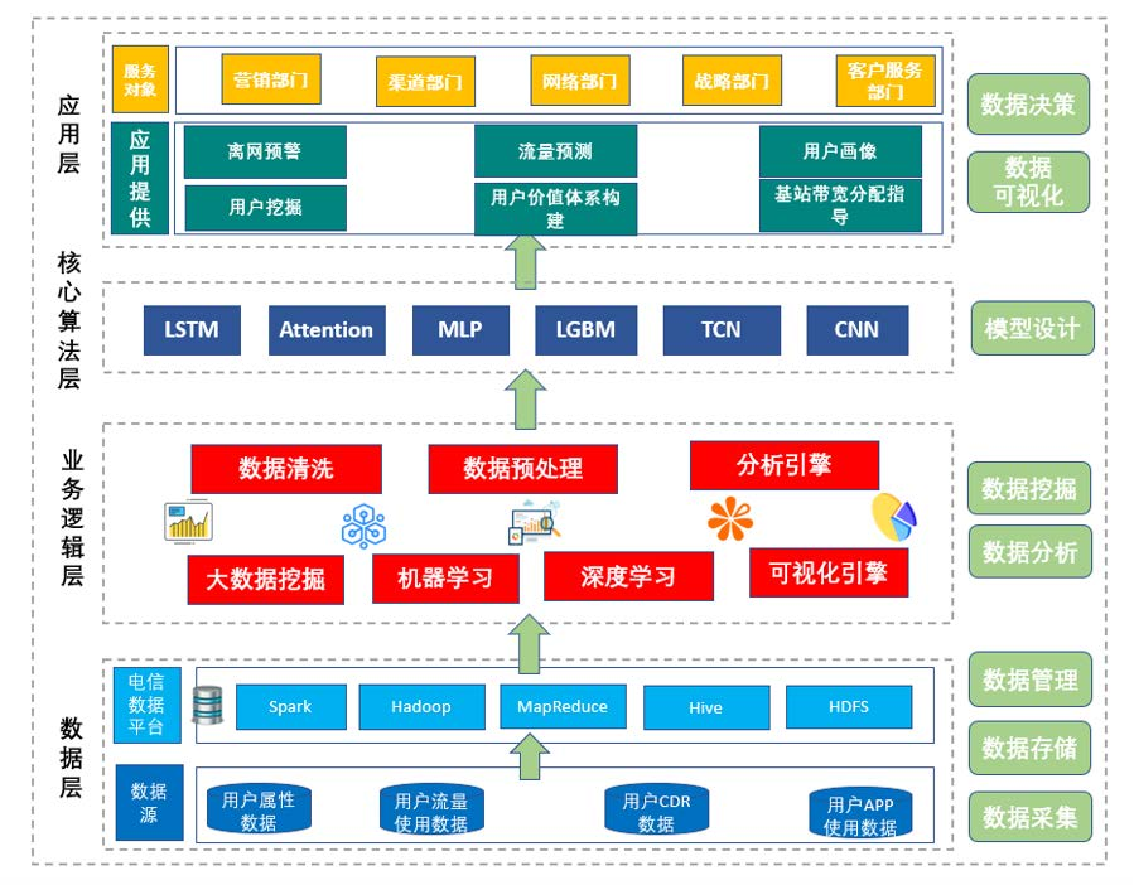
\includegraphics[width=1\textwidth]{Ms-Data_Platform.pdf}
	\caption{大数据平台系统架构}
	\label{Fig:Data-Platform}
\end{figure}

运营商们每天都会生产和存储巨量的数据,其中分为业务支持系统(BSS)和运营支持系统(OSS),这两者也构建了大数据平台的底层,从而用来提升业务和运营表现。具体来说,图\ref{Fig:Data-Platform}展示了流量运营商的大数据平台架构,其中包括数据层、业务逻辑层、核心算法层和应用层。\par
首先是数据层,数据层主要是承担数据采集、数据存储和数据管理的功能。首先从数据源中保存来自业务支持系统(BSS)和运营支持系统(OSS)的多维度数据,包括用户属性数据、用户流量使用数据、用户CDR数据、用户APP数据等。然后通过数据操作工具来做这些数据做周期性的更新、修改和删改工作从而提供给上层做其他工作。其中,Hadoop分布式文件系统(HDFS)通过分布式硬件平台来提供基础的数据存储功能。Hive/Spark SQL则是提供数据查询、清洗、过滤等功能,尤其是的提高了针对海量数据的开发和处理效率。而MapReduce则是提供大数据的并行计算范式从而缩短数据处理时间。\par
然后是业务逻辑层,次层主要为不同的业务部门提供数据分析、挖掘和建模功能。举例来说,其中包括数据预处理、统计分析、特征工程、机器学习等模块。\par
接着是核心算法层,主要是实现一些机器学习和深度学习模型的核心算法,其中包括针对表格型数据的轻度梯度提升机(LGBM)和多层感知机(MLP)等模型,针对序列数据的长短期记忆网络(LSTM)、时域卷积网络(TCN)、基于自注意力机制的深度神经网络(Transformer)等模型,针对图像的卷积神经网络(CNN)、自注意力视觉神经网络(ViT)等模型等模型。\par
最后是应用层,主要是提供经过开发人员开发和封装好的全流程自动的应用程序,为下游的营销部门、渠道部门等提供用户画像、离网预警等功能。

\subsection{数据描述}
\begin{figure}[hbt]
	\centering
	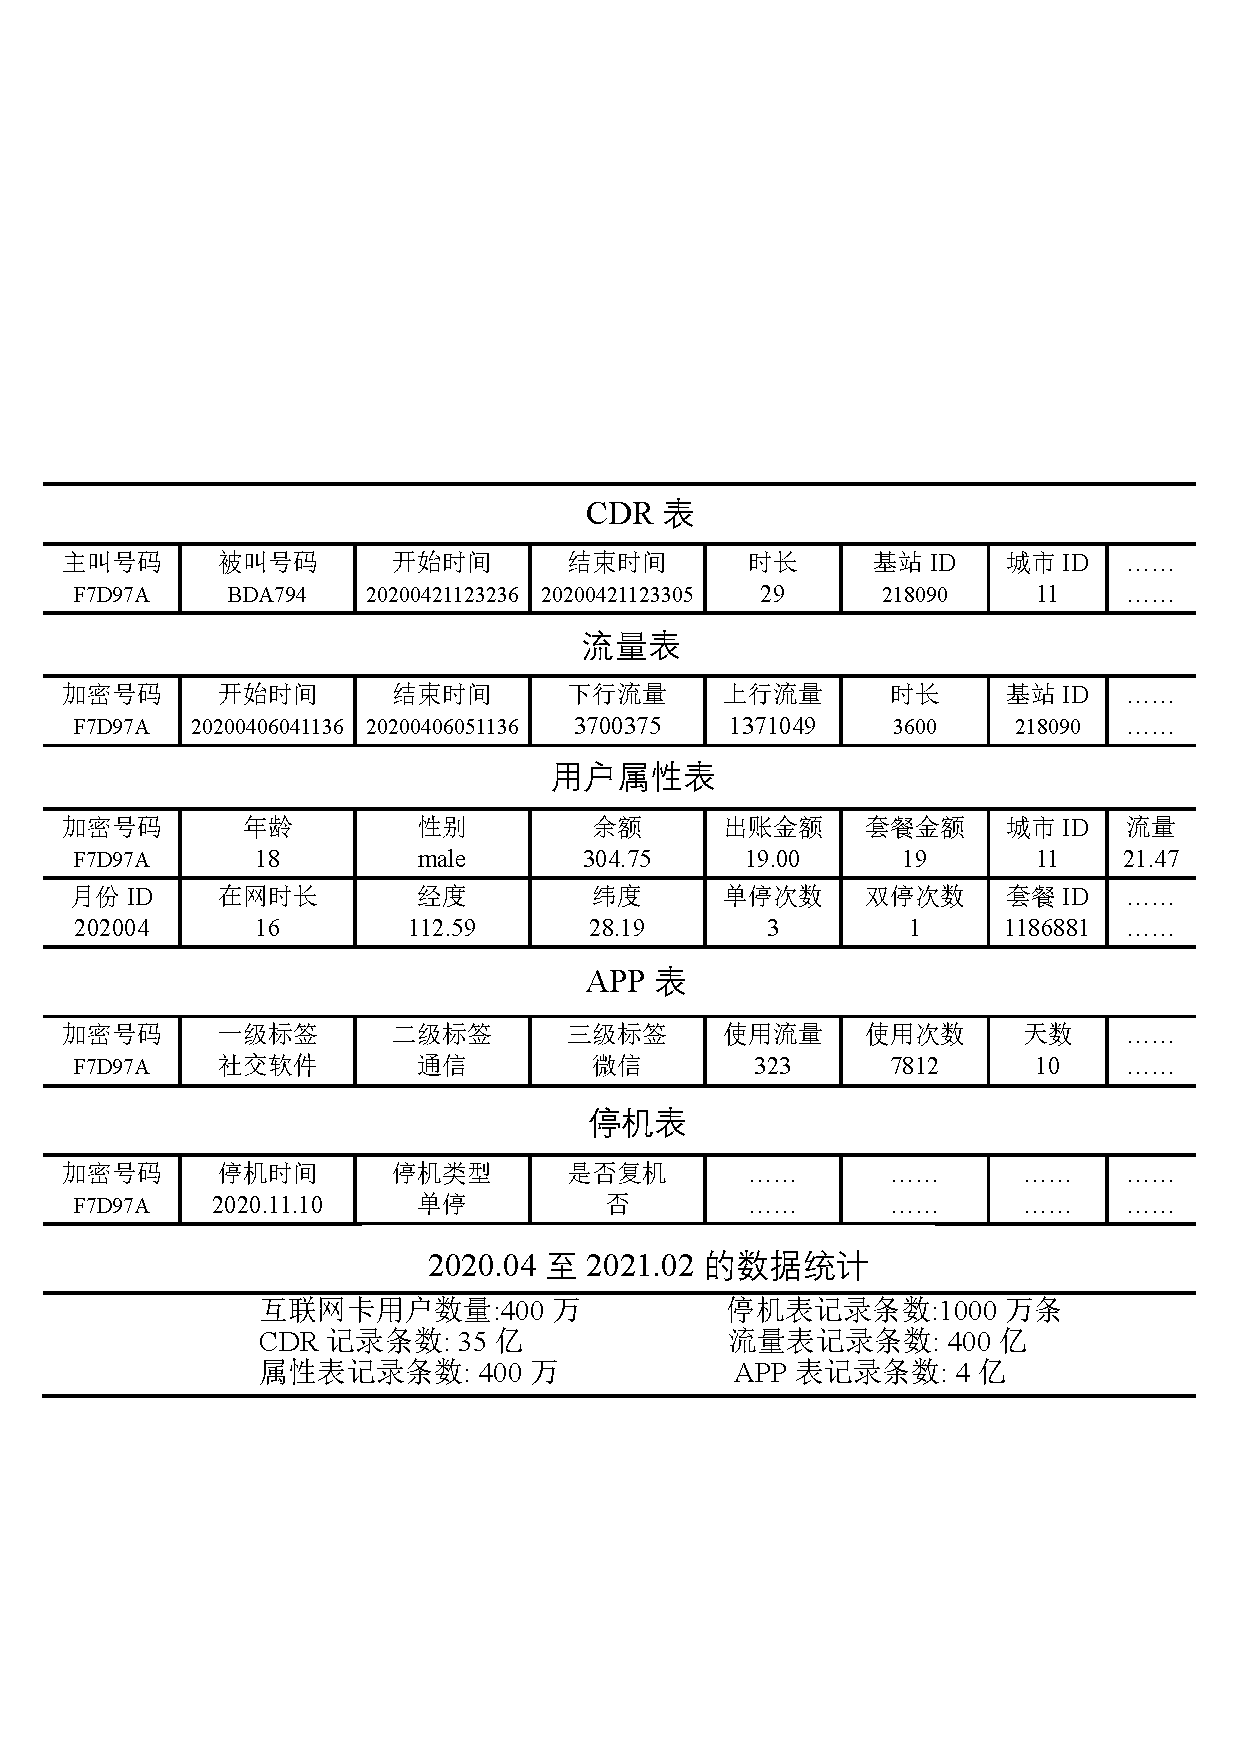
\includegraphics[width=1\textwidth]{Ms-Data_Data-Description-User_v1_1.pdf}
	\caption{用户侧数据描述}
	\label{Fig:User-Side-Data}
\end{figure}
首先, 本文来描述一下用户侧数据, 如图\ref{Fig:User-Side-Data}所示。\par
\textbf{时间范围.} 本文拥有2020年4到6月,11月到12月和2021年1到2月的7个月的数据。\par
\textbf{用户类型.} 本文过滤掉了政企用户、家庭用户和其他用户,只留下互联网卡个人用户。\par
\textbf{数据规模.} 在这7个月的数据中,一共有400万的互联网卡个人用户,400万条以月为粒度的属性表记录,35亿条以次为粒度的CDR(通话细节记录)表记录,400亿条以次为粒度的流量表记录,4亿条以月为粒度的APP(应用程度)表记录, 1000万条以次为粒度的停机表记录。
其中属性表记录的为用户属性数据,而其他四个表记录的为用户行为数据,尤其是流量表和CDR表的数据尤为珍贵,能够刻画用户的序列行为。但是从另一方面来说,如此海量的数据也给数据分析和模型训练推理带来了极大的硬件资源、方法性能、时间压力。\par
\textbf{具体字段.}\par
\textbf{数据用途.} \par
%\textbf{存储类型.} 这些数据主要是以HDFS\par

\begin{figure}[hbt]
	\centering
	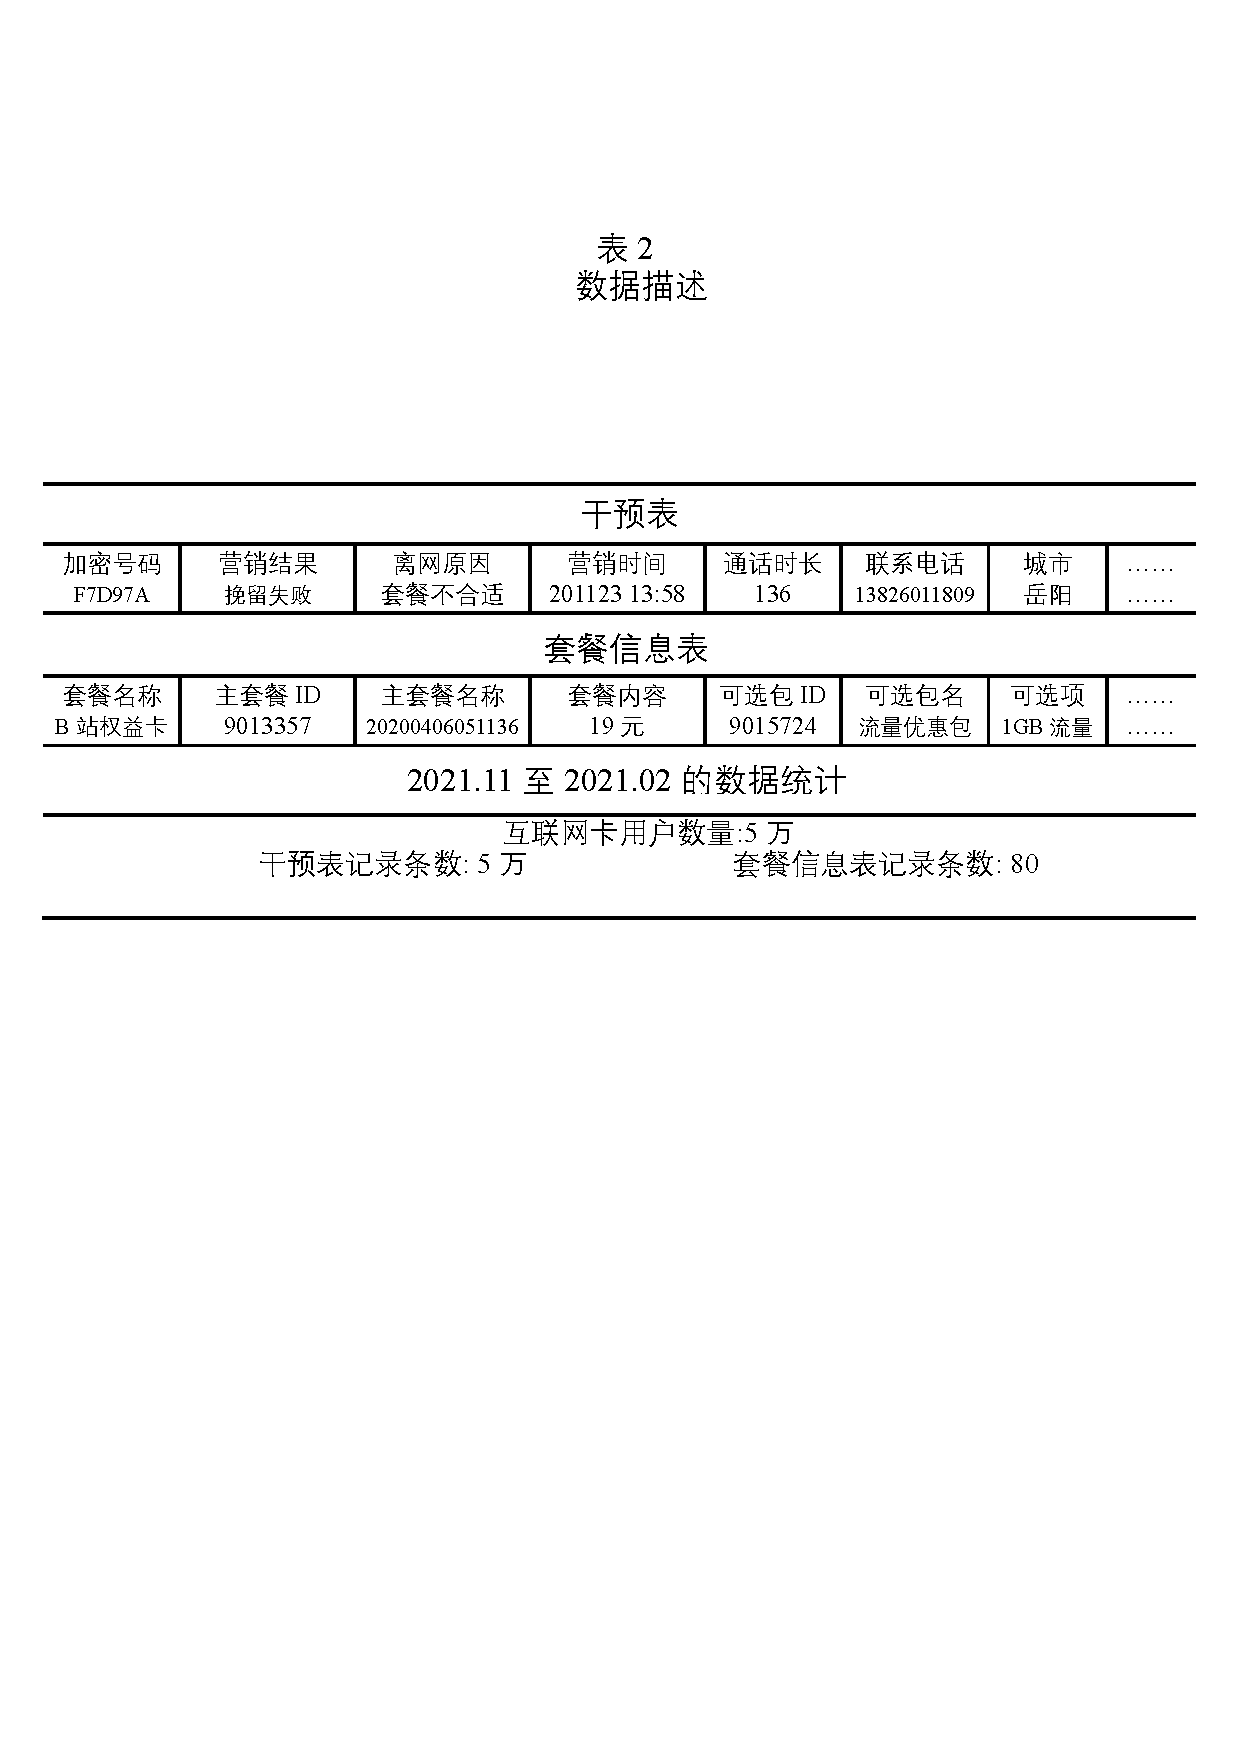
\includegraphics[width=1\textwidth]{Ms-Data_Data-Description-Item_v2_1.pdf}
	\caption{物品侧数据描述}
	\label{Fig:Item-Side-Data}
\end{figure}
接着,本文来描述物品侧数据,如图\ref{Fig:Item-Side-Data}所示。\par
\textbf{时间范围.} 本文拥有2020年11月~12月和2021年1~2月的4个月的数据。\par
\textbf{用户类型.} 本文也同样过滤掉了政企用户、家庭用户和其他用户,只留下互联网卡个人用户。\par
\textbf{数据规模.} 在这4个月的数据中,一共有20万的离网的互联网卡个人用户,20万条以次为粒度的干预表记录,80条以个为粒度的套餐信息表记录。
其中干预表记录的为运营商人工客服对离网客户的干预数据,而套餐表记录的则为互联网卡套餐的相关数据。\par
\textbf{具体字段.}\par


%\section{数据分析和特征工程}
\subsection{数据分析}
在本章中, 本文会首先针对互联网卡正常用户和离网用户做全面的数据分析,接着探索在哪些属性和行为数据上互联网卡离网用户和正常用户表现出较大差异,然后针对这些数据做相应的特征计算,提取用以区分互联网卡正常用户和离网用户的关键特征。\par
%\subsubsection{用户静态属性分析}
本文首先定义了互联网卡离网用户,然后分析了互联网卡的离网趋势以及互联网卡用户的离网原因分布。\par
\textbf{离网用户定义.}离网用户也被称为流失用户,往往是用户在使用过程中因服务不满意、资费贵、改用其他竞品等原因而选择不再使用互联网卡。其中又分为两种,分别是主动性离网和被动性离网。其中主动性离网是指用户主动到运营商营业厅提出销卡的请求,还包括退还余额等行为。而被动性离网则指用户保持了至少两周14天的双停状态,没有通过充值话费等行为使得相应手机号复机。则运营商会主动将这类号码销户,之后再销售给其他用户。本文的研究主要是针对被动性离网,因为主动性离网行为只占互联网卡所有离网行为的不到10\%,尚且不受运营商们重视。
\par
\textbf{互联网卡趋势.}
\begin{figure}[hbt]
	\centering
	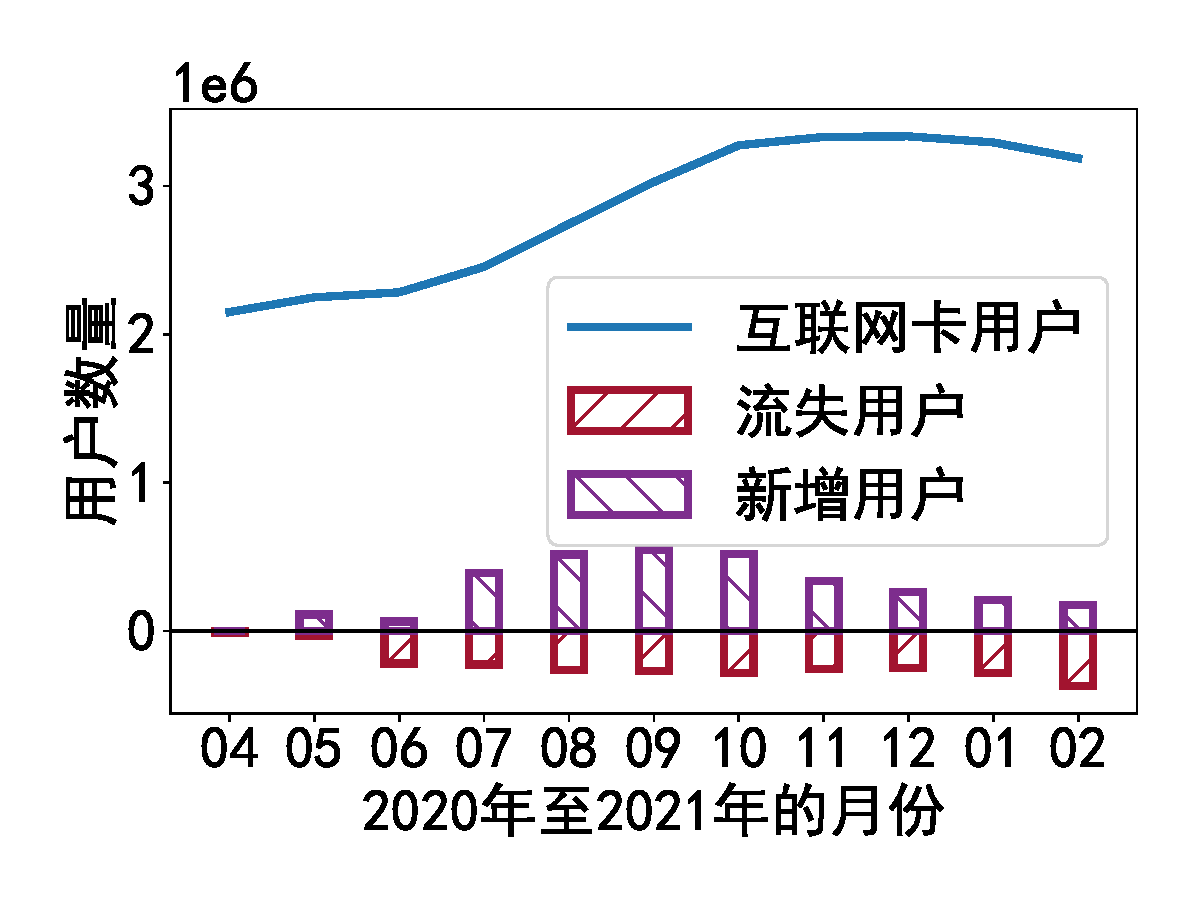
\includegraphics[width=1\textwidth]{MS-Data_IC-DevTrend_v1.pdf}
	\caption{互联网卡发展趋势}
	\label{Fig:IC-DevTrend}
\end{figure}
为了了解互联网卡这个业务的发展趋势,本文绘制了从2020年4月到2021年2月的发展趋势图,如图\ref{Fig:IC-DevTrend}所示。从图中,本文可以观察到互联网卡在初期增长得十分迅速,但是后期增长趋势放缓,从2020年4月到2021年2月一共增长了50\%的用户,数量约为100万。究其背后的原因是因为尽管在一开始互联网卡新增用户占大多数,但是随着时间流逝,离网用户的数量迅速增长,甚至超过了月新增用户。这使得离网问题变得日益严重起来,对运营商维系互联网卡业务的稳定性提出了挑战。
\par
\textbf{离网时间分析.}
\begin{figure}[hbt]
	\centering
	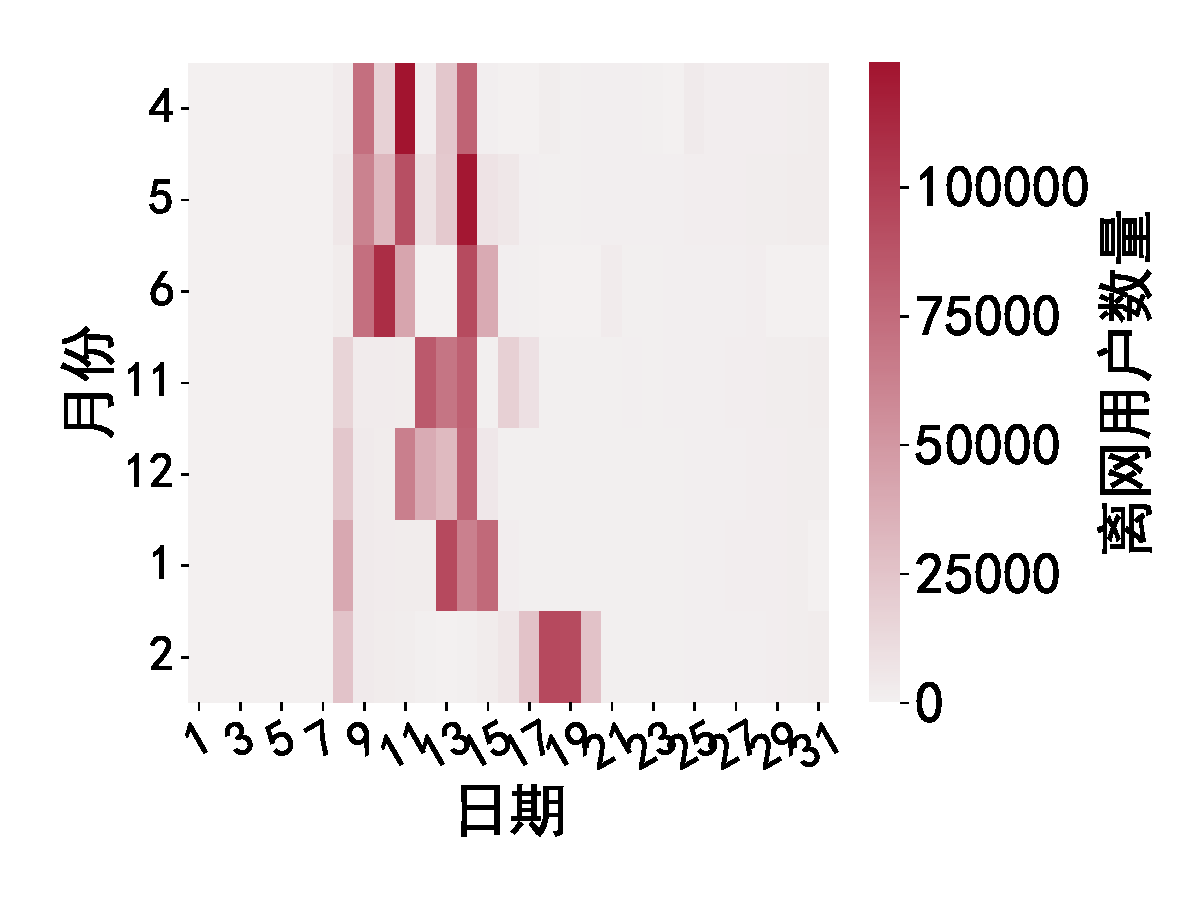
\includegraphics[width=1\textwidth]{Ms-Data_Churner-Month-Date_v1.pdf}
	\caption{互联网卡离网用户-日期热力图}
	\label{Fig:Churner-Month-Date}
\end{figure}
为了进一步地理解互联网卡用户的离网行为,本文分析了互联网卡用户7个月的停机数据并分析了每个用户的离网时间。图\ref{Fig:IC-DevTrend}展示了7个月份内不同日期的离网用户数量,本文可以观察到在每个月的9号至19号拥有绝大多数的离网用户(超过了95\%)。本文还可以发现不同月份的离网用户数量和离网时间分布具有一定差异。举例来说,2021年1月14日的离网用户数量可以达到122029个,然而其他月份只有更少的离网用户。此外,本文还观察到在每个月的月初和月末都基本没有互联网卡用户离网。这可能是与运营商的工作特点有关联,运营商的每个月初和月末常常需要做些清点工作。上述发现带给本文两个启示,首先,由于用户的离网行为在每月都有相同和不同之处,不是非常稳定,这带给整个系统的建模带来了一定挑战。其次,这也启示本文互联网卡用户偏好在月中离网,因此本文应当在上月末或者当月初就完成当月互联网卡的离网用户预测,才对运营商有实际意义。又因为互联网卡庞大的用户体量,运营商只能在每月初才能完成对所有数据的采集和基本处理工作,因此本文的工作最终也是在每月月初进行推理和产出的。


\textbf{离网原因分析.}
\begin{figure}[hbt]
	\centering
	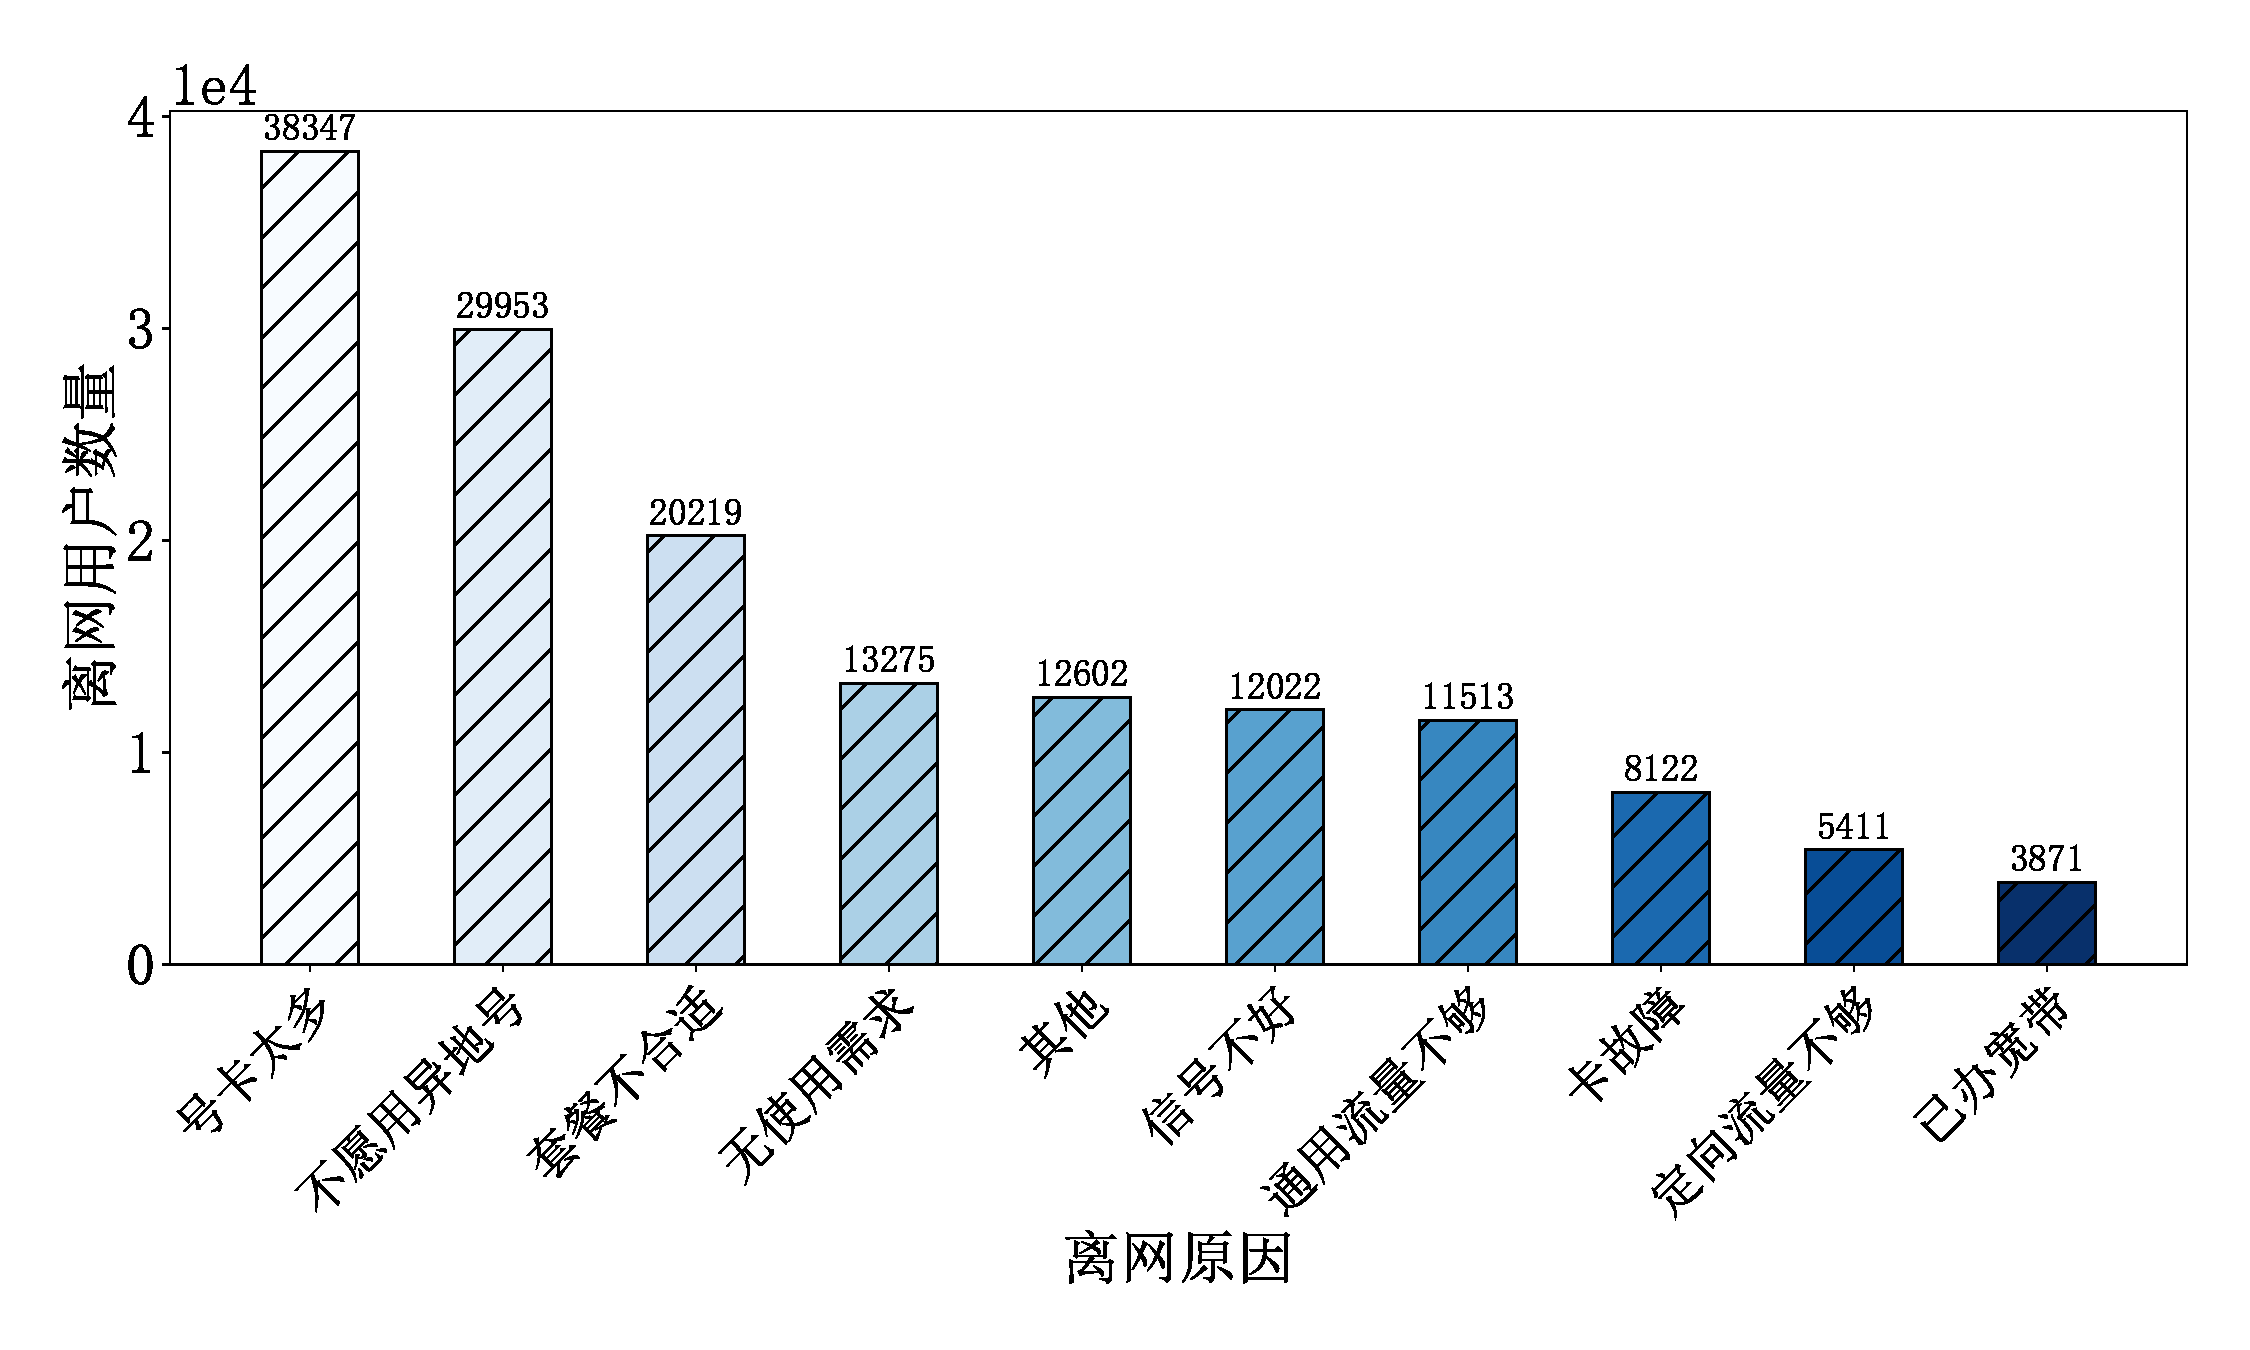
\includegraphics[width=1\textwidth]{Ms-Data_Top10-Churn-Reason_v2.pdf}
	\caption{互联网卡用户Top10离网原因}
	\label{Fig:Top10-Churn-Reason}
\end{figure}
为了理解为什么一部分互联网卡用户倾向于俩王,本文基于运营商客服收集的离网反馈分类了用户离网原因。图\ref{Fig:Top10-Churn-Reason}展示了互联网卡用户离网的数量最大的前10个原因。本文可以看到互联网卡用户最多是因为“号卡太多”这个原因离网的。因为现在不同的运营商都在计划占据整个互联网卡市场。他们通过向新用户频繁宣传和给予大量折扣的优惠来吸引他们使用自家的互联网卡。因此,部分互联网卡用户可能会被其他运营商的优惠政策所吸引,从而离网转向使用他运营商的互联网卡。第二大离网原因是互联网卡用户不愿使用异地号。因为运营商的不同省份都是各自独立的,都会向全国各地兜售互联网卡。因此部分互联网卡用户使用的互联网卡的负责公司所出的省份与自己所处的省份并不同,在接听和拨打电话时常常会引起误会,而这个现象则会导致部分用户不想使用异地的互联网卡。并且由于异地的关系,手机信号和网络可能变得不稳定,从而影响用户的使用体验。此外,套餐不合适和无使用需求也占据了相当大的比例,这些是能被运营商优化的。从长期来说,互联网卡用户和原因的分布随着时间流逝和新用户的加入可能会变得不同。因此,本文只关注用户离网原因的类别。然后,本文可以为不同离网原因类别设计相应的干预策略从而挽留住那些已经离网或者将要离网的互联网卡用户。总的来说,用户离网原因分布的改变并不会影响系统的总体性能。\par
因为运营商通过向互联网卡用户收取基本的套餐费用以及额外的服务费用来赚取利润的,所以互联网卡这个业务市场高度依赖于互联网卡用户的数量。因为用户离网问题对运营商来说至关重要,所以本文设计和实现的系统不得不理解互联网卡离网用户的潜在行为并且提前预测用户的离网行为从而发起早期的干预。因此,本文迫切需要了解互联网卡用户画像,在此基础上制定更有效的业务策略,防止他们离网,这也是本工作的动力之一。
\par
%接着本文针对用户的静态属性进行了对比性的数据分析。


%\subsubsection{用户时序行为分析}
%
%
%\subsubsection{用户异常行为分析}


\subsection{特征工程}
在本小节中,本文会展示基于数据分析的一些重要特征,主要分成两类,一类是静态画像特征,另一类是时间序列特征。
\subsubsection{静态特征工程}
\textbf{账户余额.}
\begin{figure}[hbt]
	\centering
	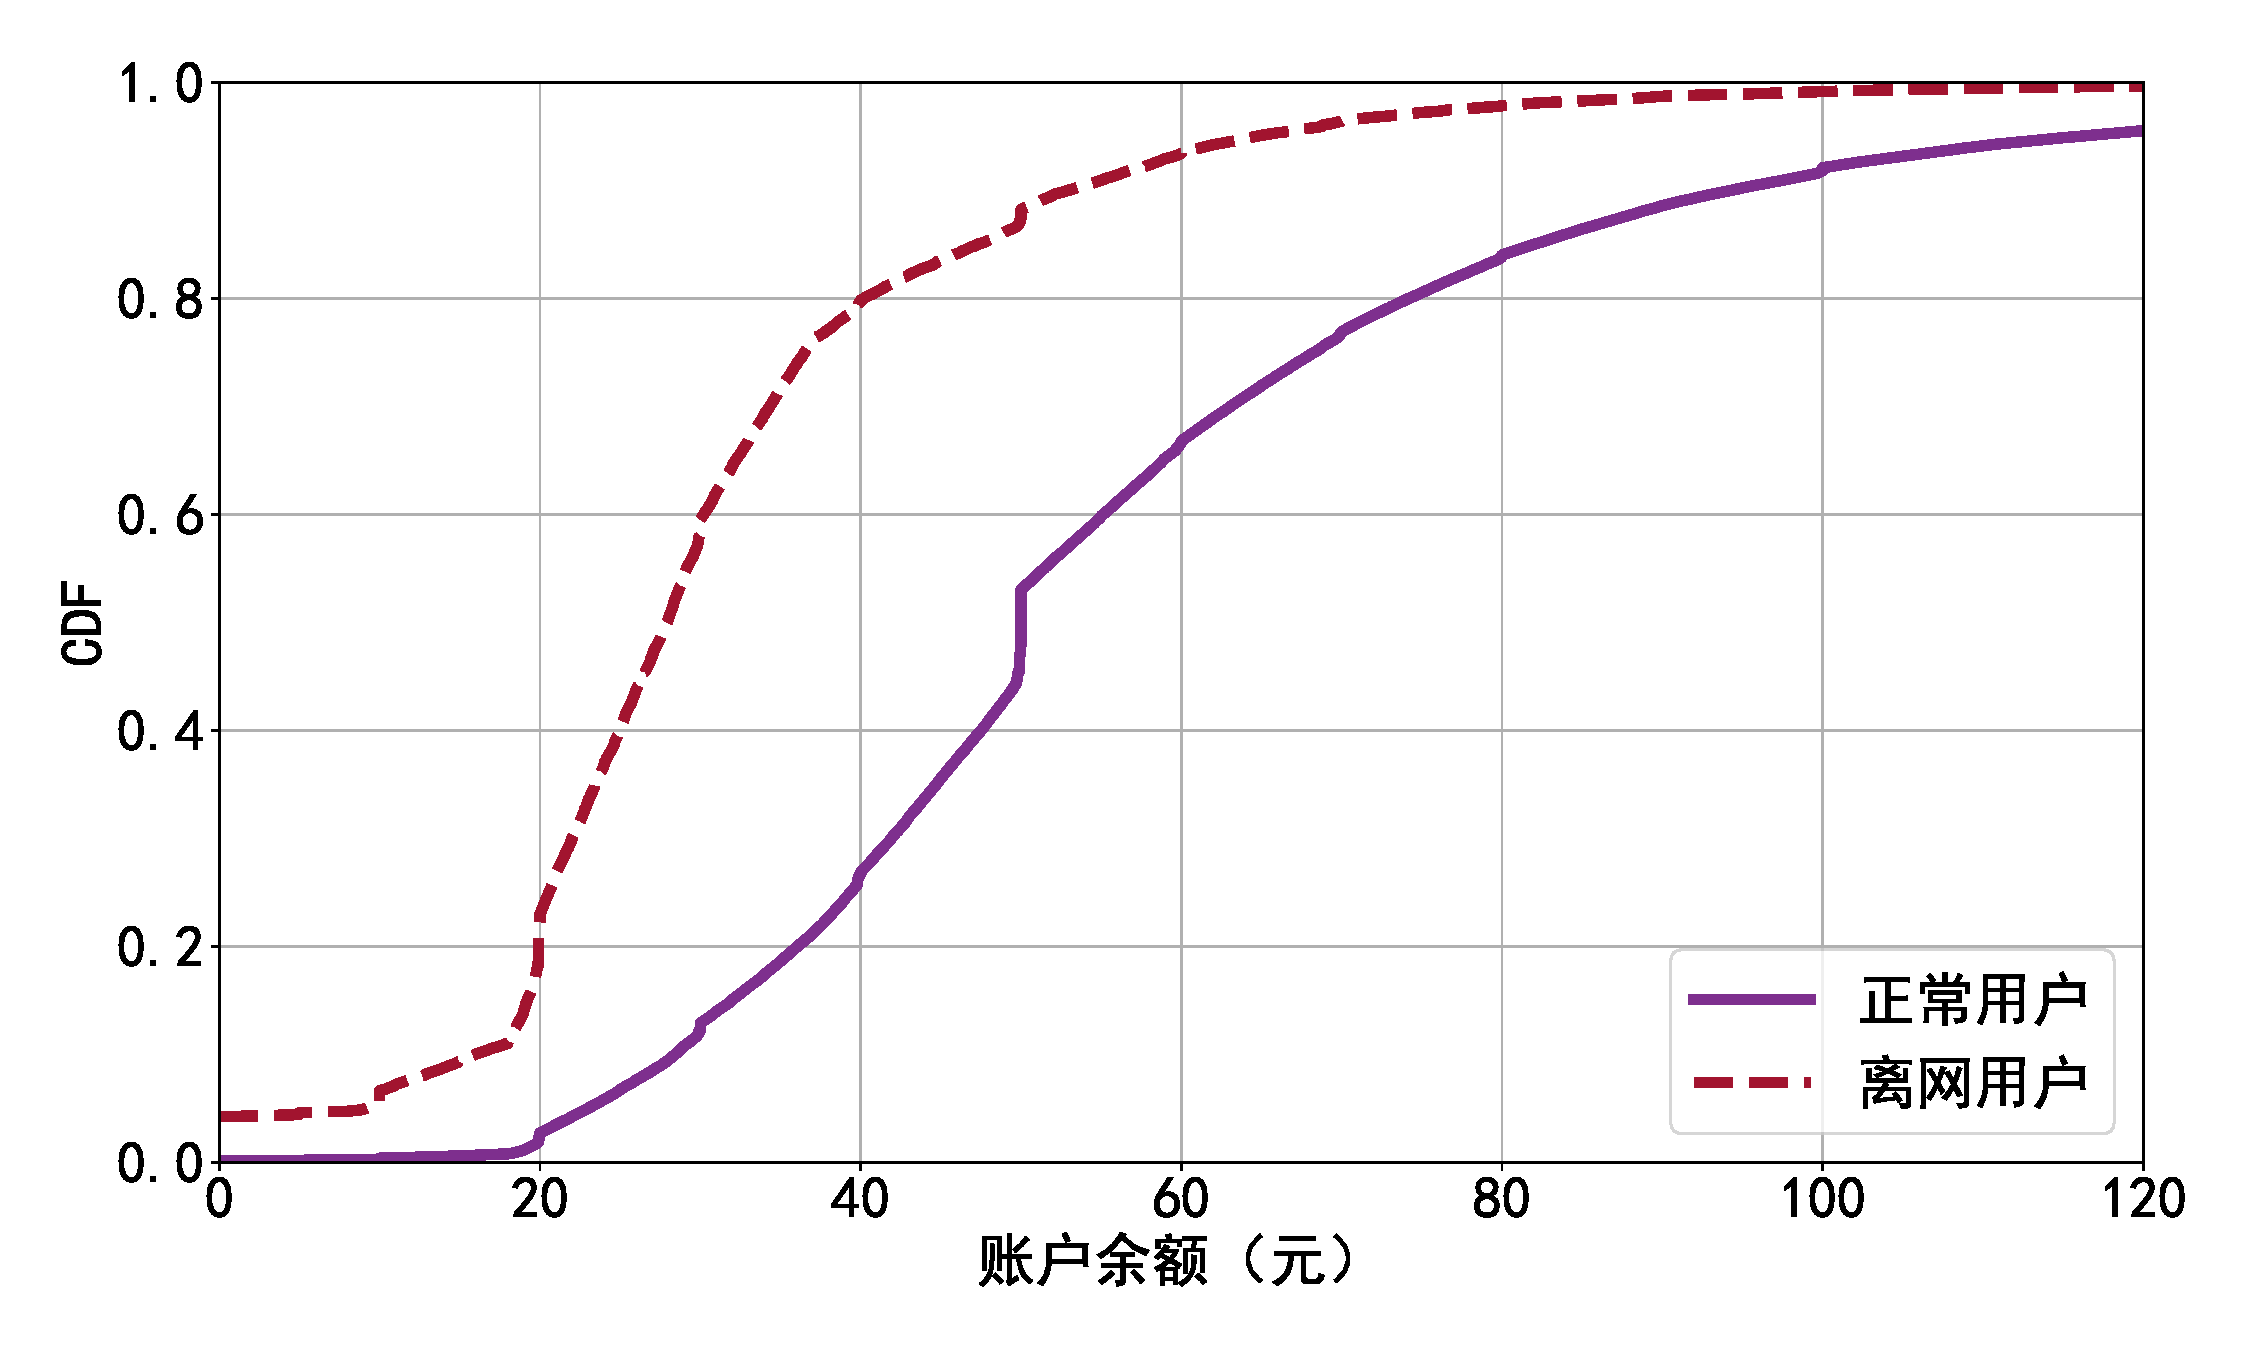
\includegraphics[width=1\textwidth]{Ms-Data_Balance.pdf}
	\caption{互联网卡用户账户余额对比}
	\label{Fig:Balance}
\end{figure}
当互联网卡用户即将离网的时候,他们通常倾向于花光账户里的余额,因此账户余额越低,用户越容易离开运营商。图\ref{Fig:Balance}展示了互联网卡正常用户和离网用户的累积分布函数(CDF)图,可以看出这两条曲线有着非常大的差距。详细来说,对于80\%的用户来说,离网用户的账户余额都小于40元,而正常用户的账户余额都小于75元,这意味着账户余额在用户发生离网行为前是一条关键的线索。

\par

\textbf{平均流量消耗阶段.}
\begin{figure}[hbt]
	\centering
	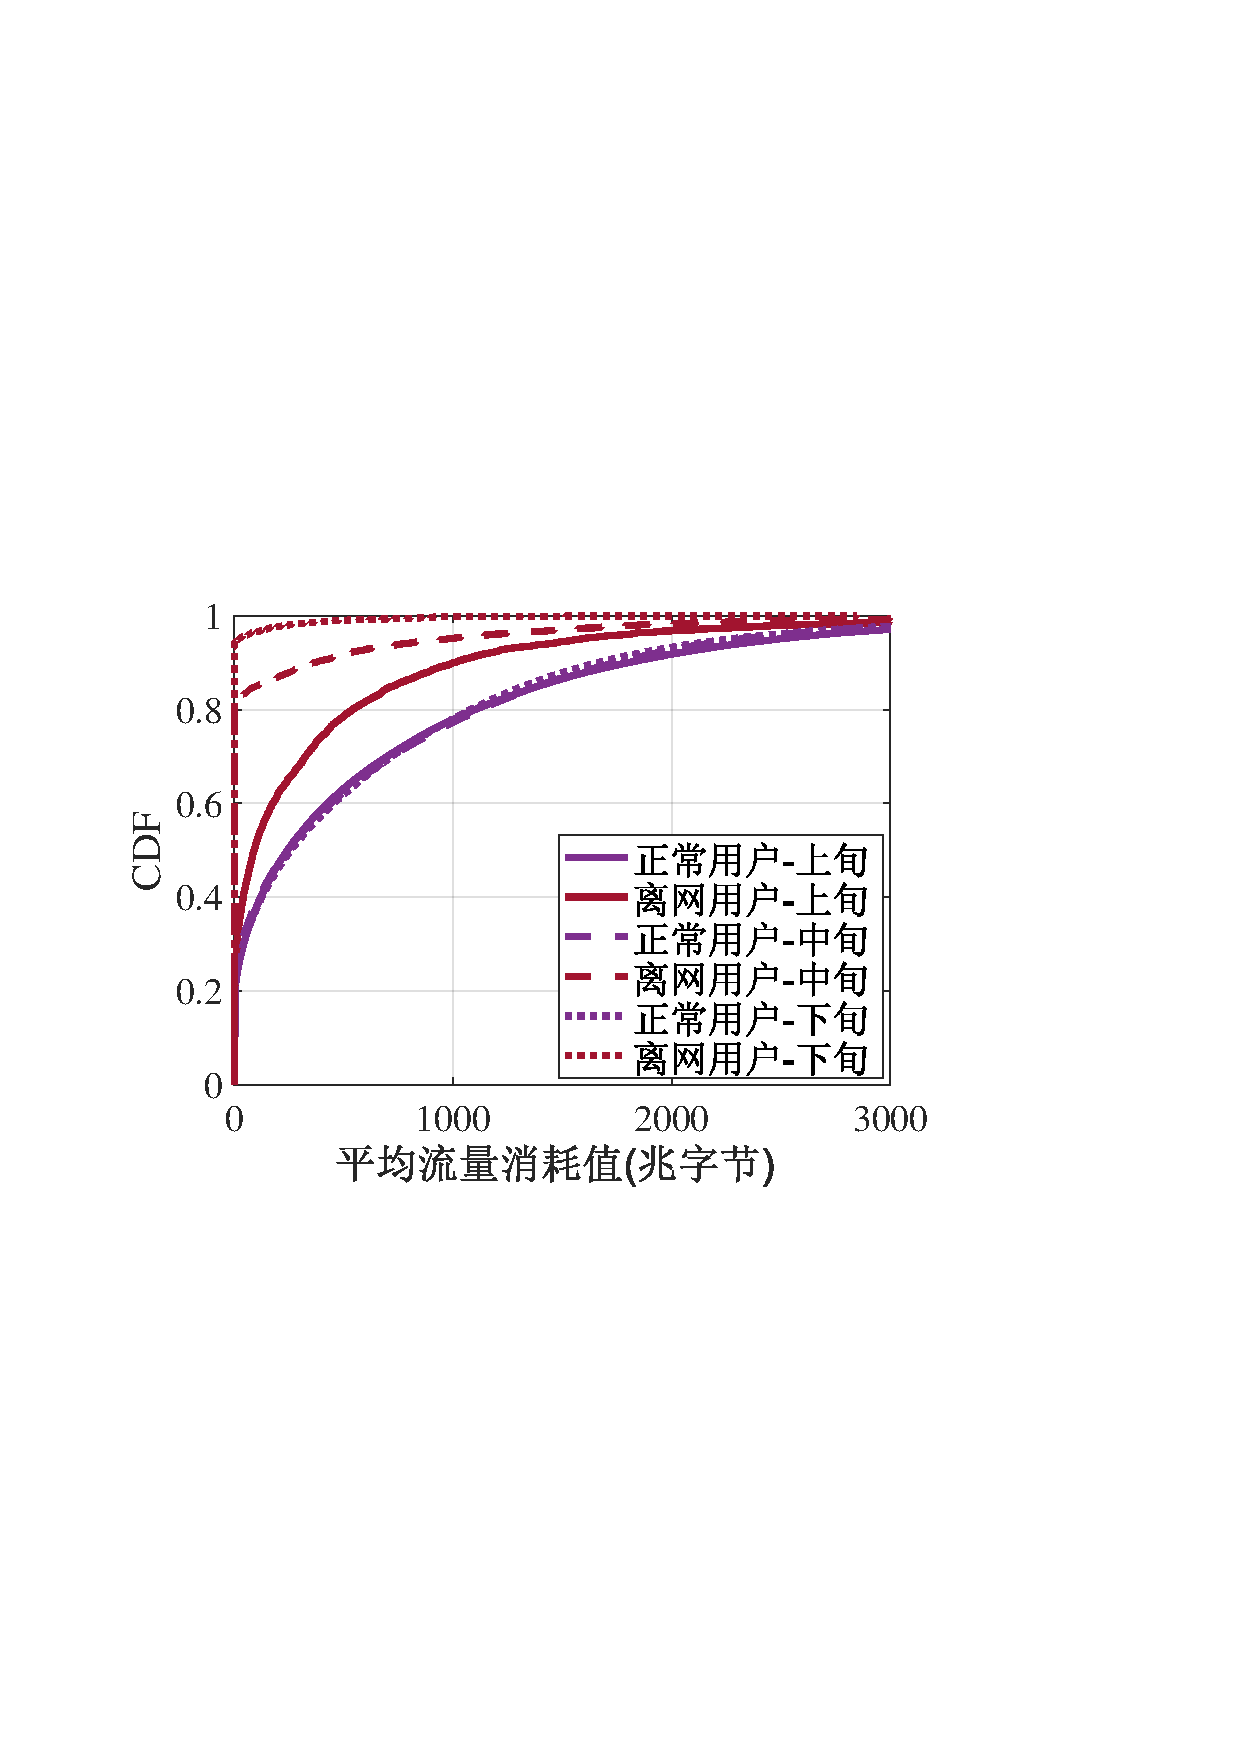
\includegraphics[width=1\textwidth]{Ms-Data_Traffic-Stage_1.pdf}
	\caption{月不同阶段的互联网卡用户平均消耗流量值对比}
	\label{Fig:Traffic-Stage}
\end{figure}
对于即将离网的用户来说,他们的网络行为往往会发生变化。为了捕捉这个特征,本文把每个月份平均分成三个等长的阶段,分别是上旬,中旬和下旬。图\ref{Fig:Traffic-Stage}显示了正常用户和离网用户在月份不同阶段的流量消耗变化。从中可以观察到对于正常用户来说,平均流量消耗并没有什么区别。但是在离网用户的三个不同阶段,流量消耗曲线有很明显的差距。举个例子,在上旬,中旬和下旬,平均消耗流量为0的用户在所有离网用户占比分别达到了30\%,80\%和96\%。
\par

\textbf{APP使用频次.}
\begin{figure}[hbt]
	\centering
	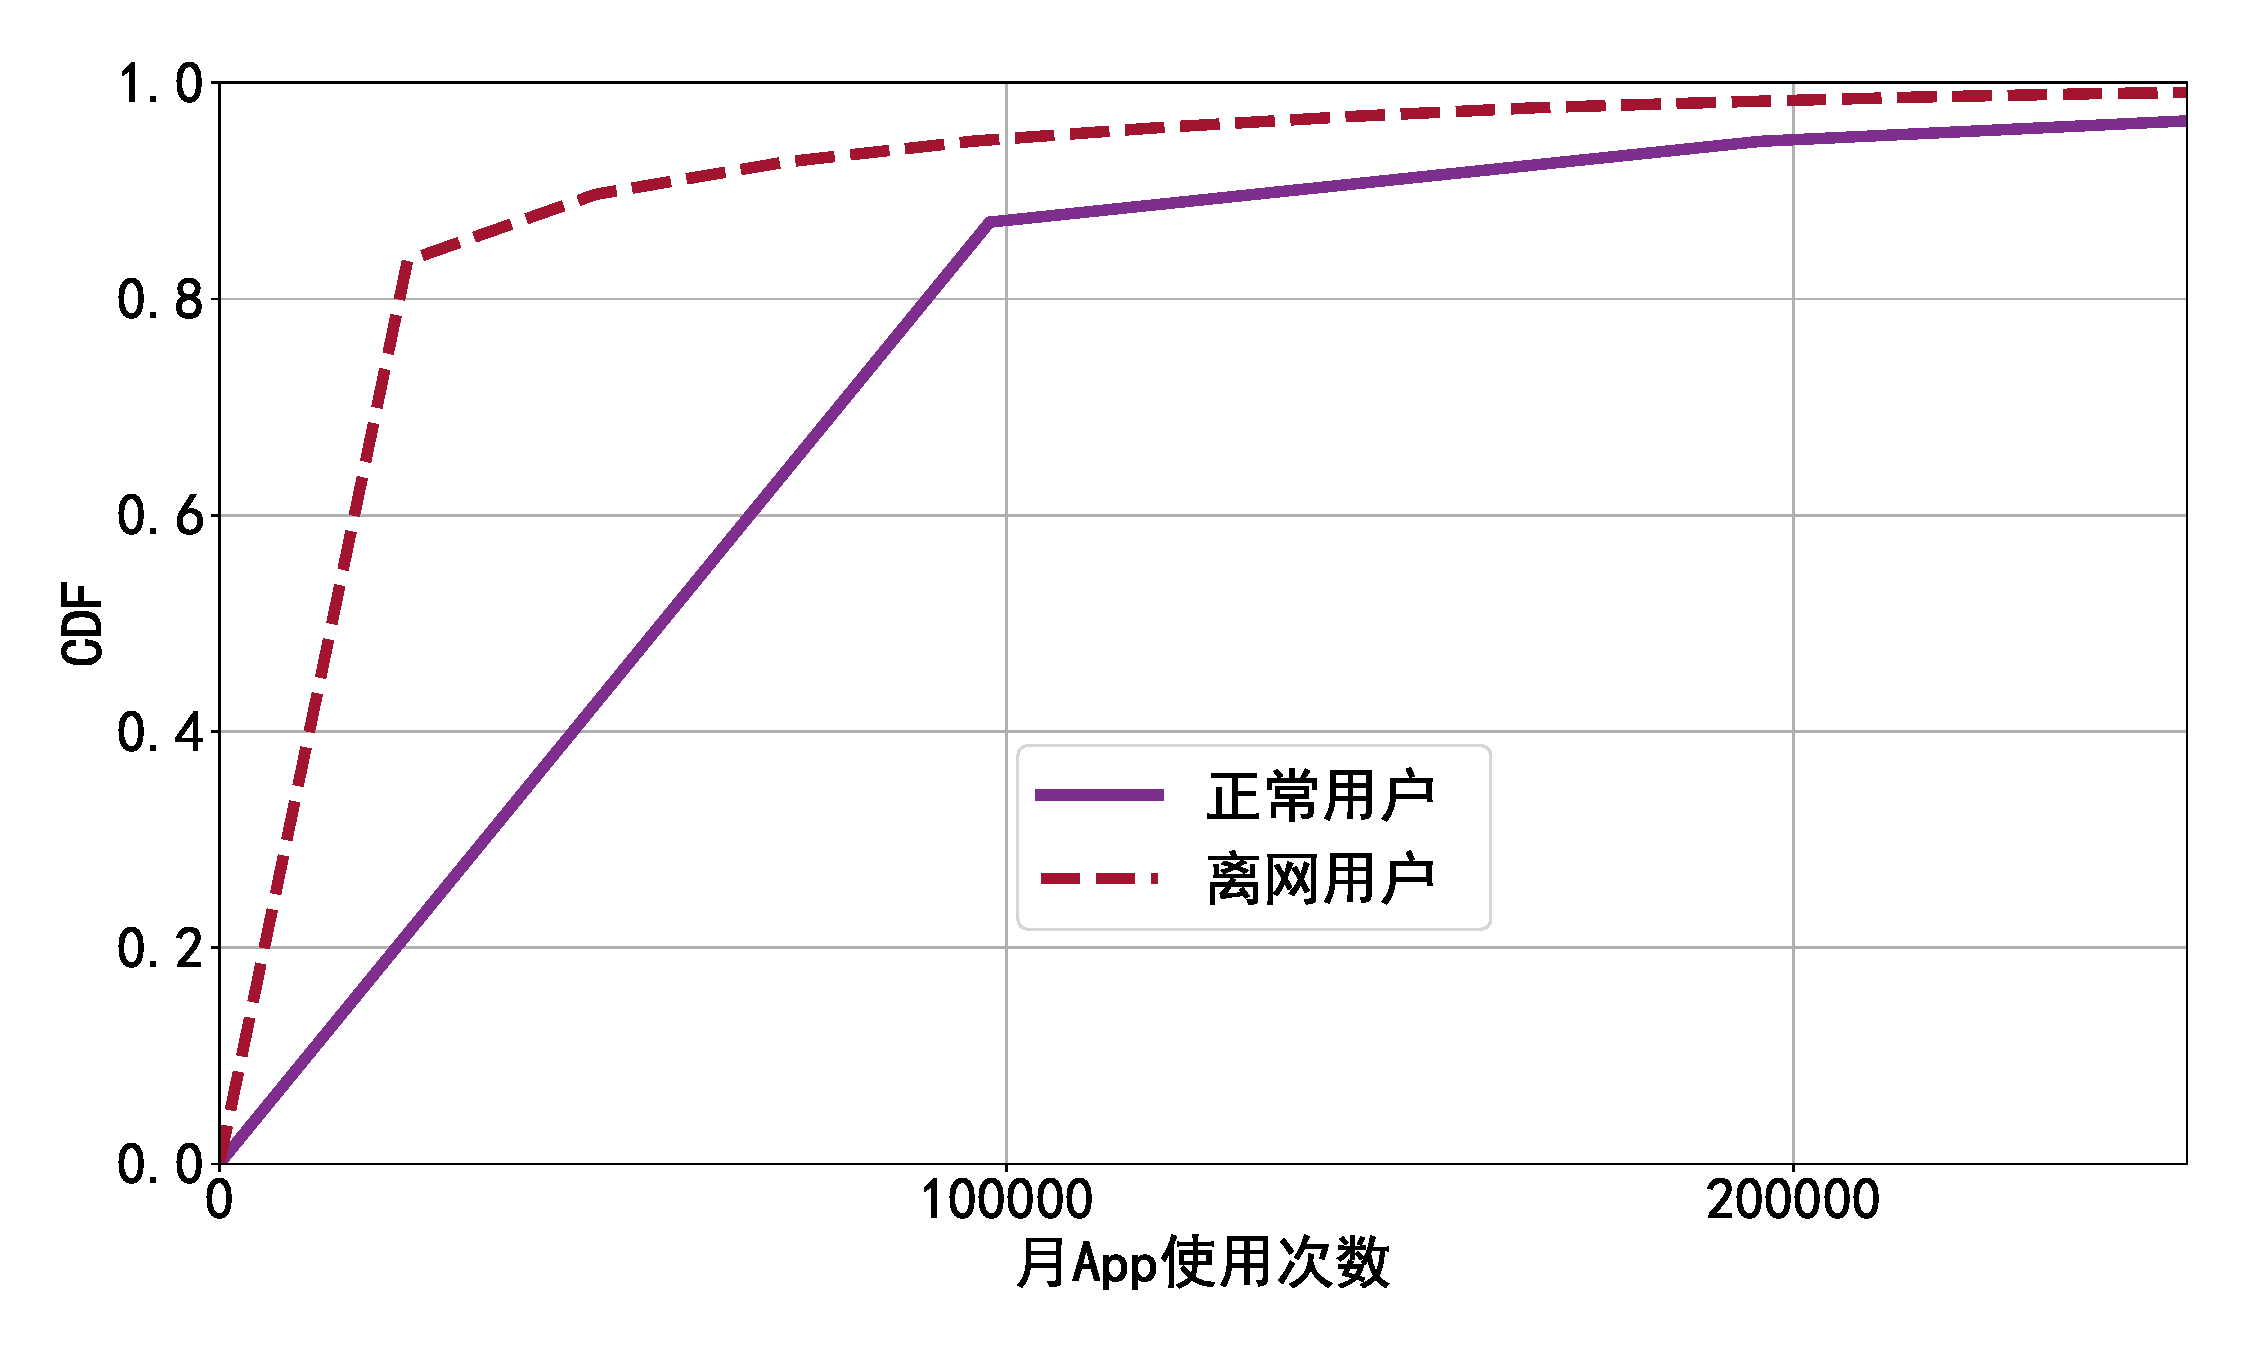
\includegraphics[width=1\textwidth]{Ms-Data_App-Use-Times.pdf}
	\caption{互联网卡用户月APP使用频次对比}
	\label{Fig:App-Use-Times}
\end{figure}
为了捕捉互联网卡用户的APP使用习惯,本文基于采集的APP表计算了每个互联网卡用户在一个月内的所有APP使用频次。在图\ref{Fig:App-Use-Times}中,本文描绘了正常用户和离网用户关于APP使用频次的对比CDF图,并且其中有非常大的不同。具体来说,正常用户的APP使用频次的中位数是36075次,而离网用户的对应中位则是18442次。这意味着APP使用频次对于互联网卡用户来说是一个非常有价值的特征用以区别正常用户和离网用户。
\par




\textbf{活跃熵.}
\begin{figure}[hbt]
	\centering
	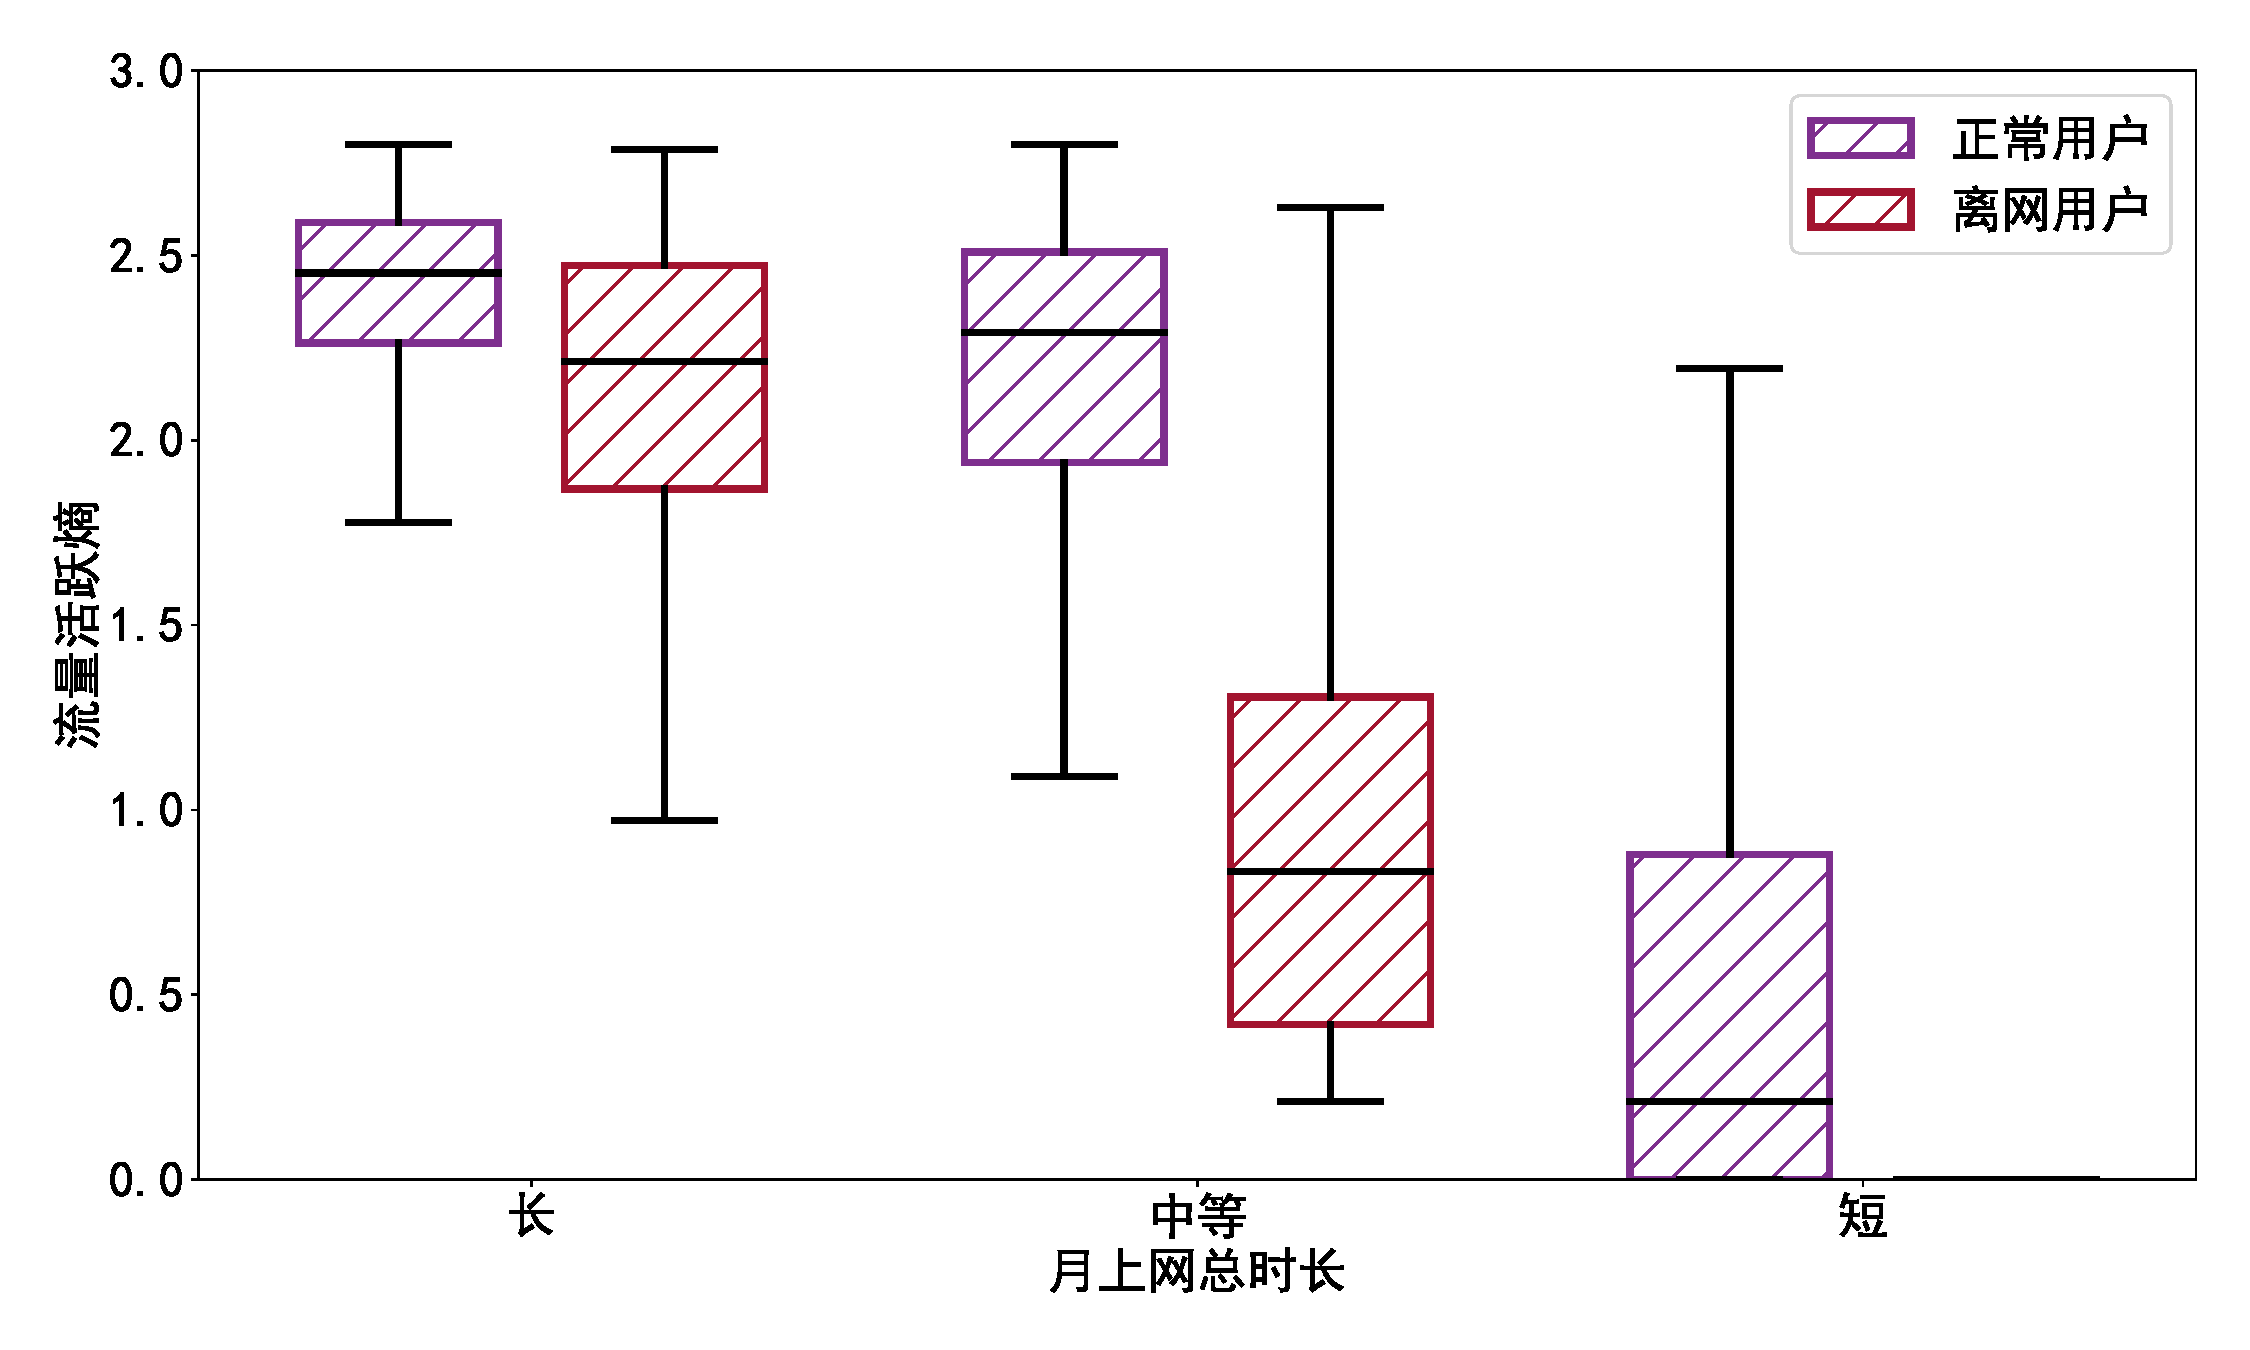
\includegraphics[width=1\textwidth]{Ms-Data_Traffic-Active-Entropy.pdf}
	\caption{互联网卡用户流量活跃熵对比}
	\label{Active-Entropy}
\end{figure}

和上述思路保持一致,本文基于香农信息熵探索了在一个月内日指标观察值(包括,使用流量大小,流量记录条数,上网时长等)的不确定性。对于某个互联网卡用户$u$来说,他关于上网时长序列的活跃熵$H(D_{u})$可以被如下公式\eqref{Eq:Active-Entropy} 计算。
\begin{equation}
	H(D_{u}) = \sum_{k=0}^{min(maxbin, len(D_{u}))} p_{k} \log \frac{1}{p_{k}}
	\label{Eq:Active-Entropy}
\end{equation}
其中$D_{u}$是用户$u$的上网时长序列,$p_{k}$表示上网时长序列中的数值落在第k个箱子的概率。此外,$max_bin$是分箱的数量,$len(D_{u})$是$D_{u}$的长度。如果上网时序列的活跃熵比较大,这意味着上网时长序列中的数值在区间$[min(D),max(D)]$中更为分散和混乱。否则,如果上网时序列的活跃熵比较小,这意味着上网时长序列中的数值都集中在某个较小的确定区间内。在图\ref{Active-Entropy}中,本文同时绘制了正常用户和离网用户关于日上网时长活跃熵的箱线图。并且用户们被分成了三组,分别是上网时长较长,上网时长中等和上网时长较短。本文可以观察到两种类型用户的不同行为模式,其中离网用户有着更小的熵值,这显示了他们有这更简单的网络行为模式,从而使得他们能够同正常用户区分开来。


\textbf{目标编码.}
\begin{figure}[hbt]
	\centering
	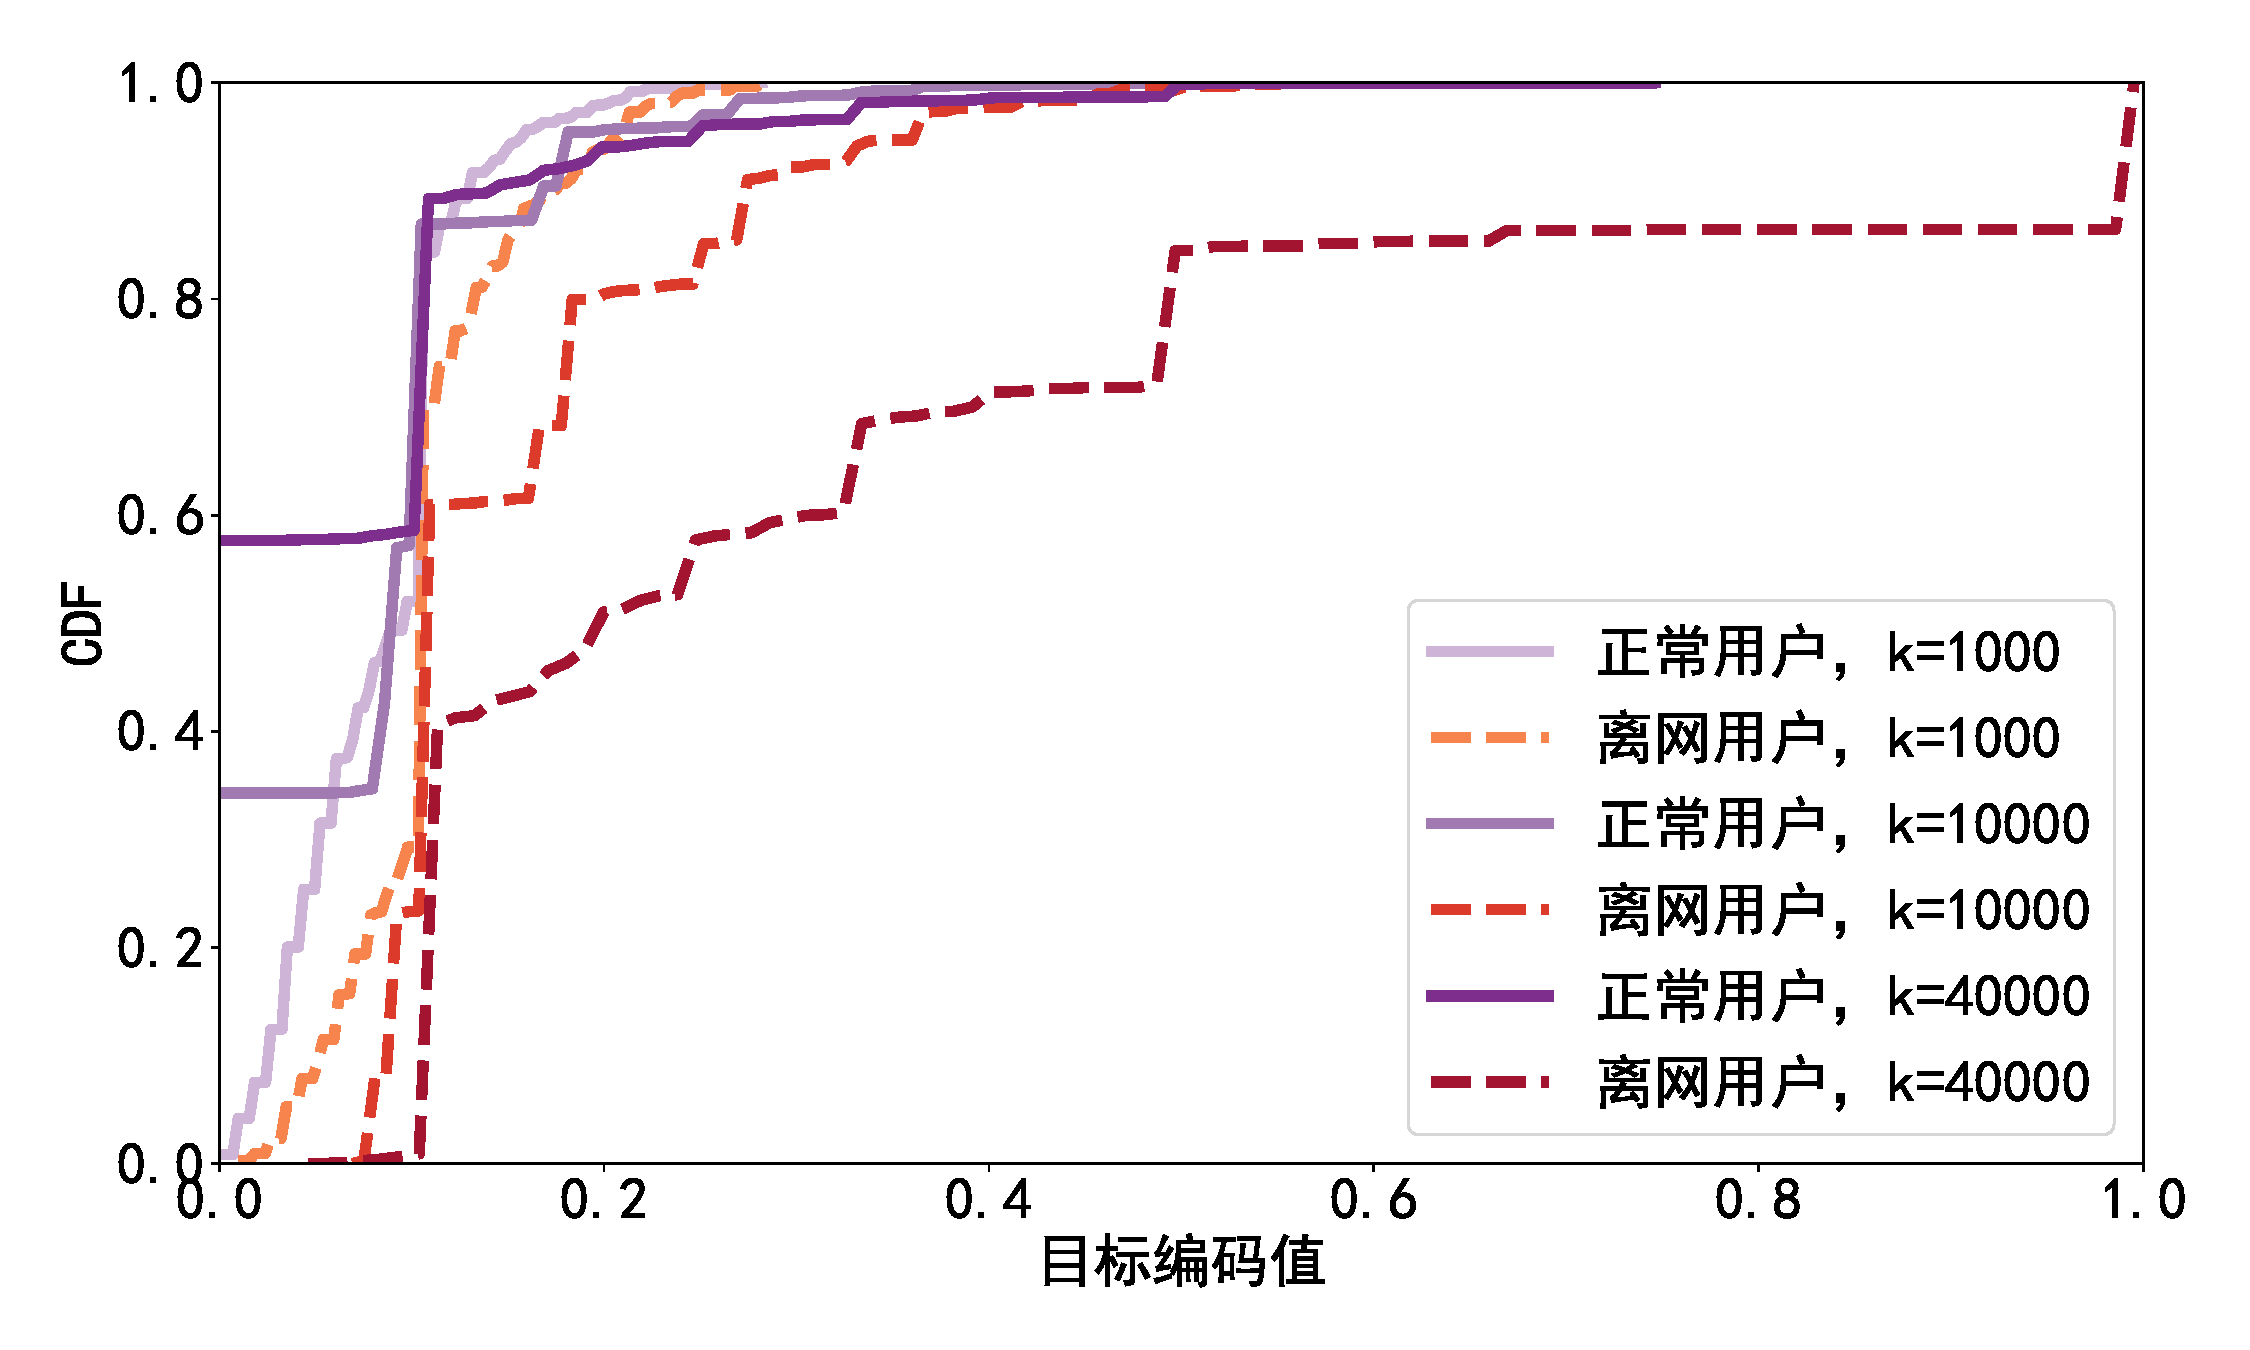
\includegraphics[width=1\textwidth]{Ms-Data_Target-Encoding-K.pdf}
	\caption{互联网卡用户目标编码值对比}
	\label{Fig:Target-Encoding-K}
\end{figure}
为了构建目标编码,比如将分类特征替换为相应目标的后验概率,本文首先根据用户的流量消耗值将互联网卡用户分组。特别地,本文将流量数据等宽地平均分到了k个箱子中,每个箱子的宽度($w$)等于
\begin{equation}
	w = (Max-Min)/k
	\label{Eq:bin-width}
\end{equation}
其中Max和Min分别代表了用户在一个月内的总流量使用值的最小值和最大值,并且每个箱子的边界值分别是$\{Min+w,Min+2w,...,Min+(k-1)w\}$。
因此,针对流量分箱的目标编码值,比如以符号$\vec{R}$表示,可以被如下公式\eqref{Eq:Target-Encoding}计算
\begin{equation}
	\vec{R} = Concat(\frac{\sum_{j=1}^{n_{i}}u_{ij} \cdot y_{ij}}{n_{i}}), i=1,2,...,k,
	\label{Eq:Target-Encoding}
\end{equation}
其中$n_{i}$表示在第i个箱子中的用户数量,$u_{ij}$表示在第i个箱子中的第j个用户,$y_{ij} \in \{0,1 \}\}$表示目标值,比如,$y_{ij}=1$表示这个用户是离网用户,否则,这个要用户就是正常用户、此外,$Concat$函数用于拼接k个值到向量$\vec{R}$中。图\ref{Fig:Target-Encoding-K}描绘了在分箱数量不同时正常用户和离网用户的目标编码值的CDF对比图。本文可以观察到,当k=1000时,离网用户和正常用户之间的差距还不是特别明显。但是,当分箱数量增加的时候,比如k=40000时,一个良好的性能差距浮现出来,这也意味着正常用户和离网用户被分发到不同的箱子后计算的目标编码值可以有效地区分两者。\\
值得注意的是,除了上述提到的重要特征,其他基础画像特征,比如年龄、性别、开卡日期和终端类型等也被提取和注入到模型当中了。


\subsubsection{时序特征工程}
除了静态特征,时序特征对于学习模型来说也是非常重要的因为离网行为通常是一个渐进进程而不是一个突发事件。\\

\textbf{流量序列.}
\begin{figure}[hbt]
	\centering
	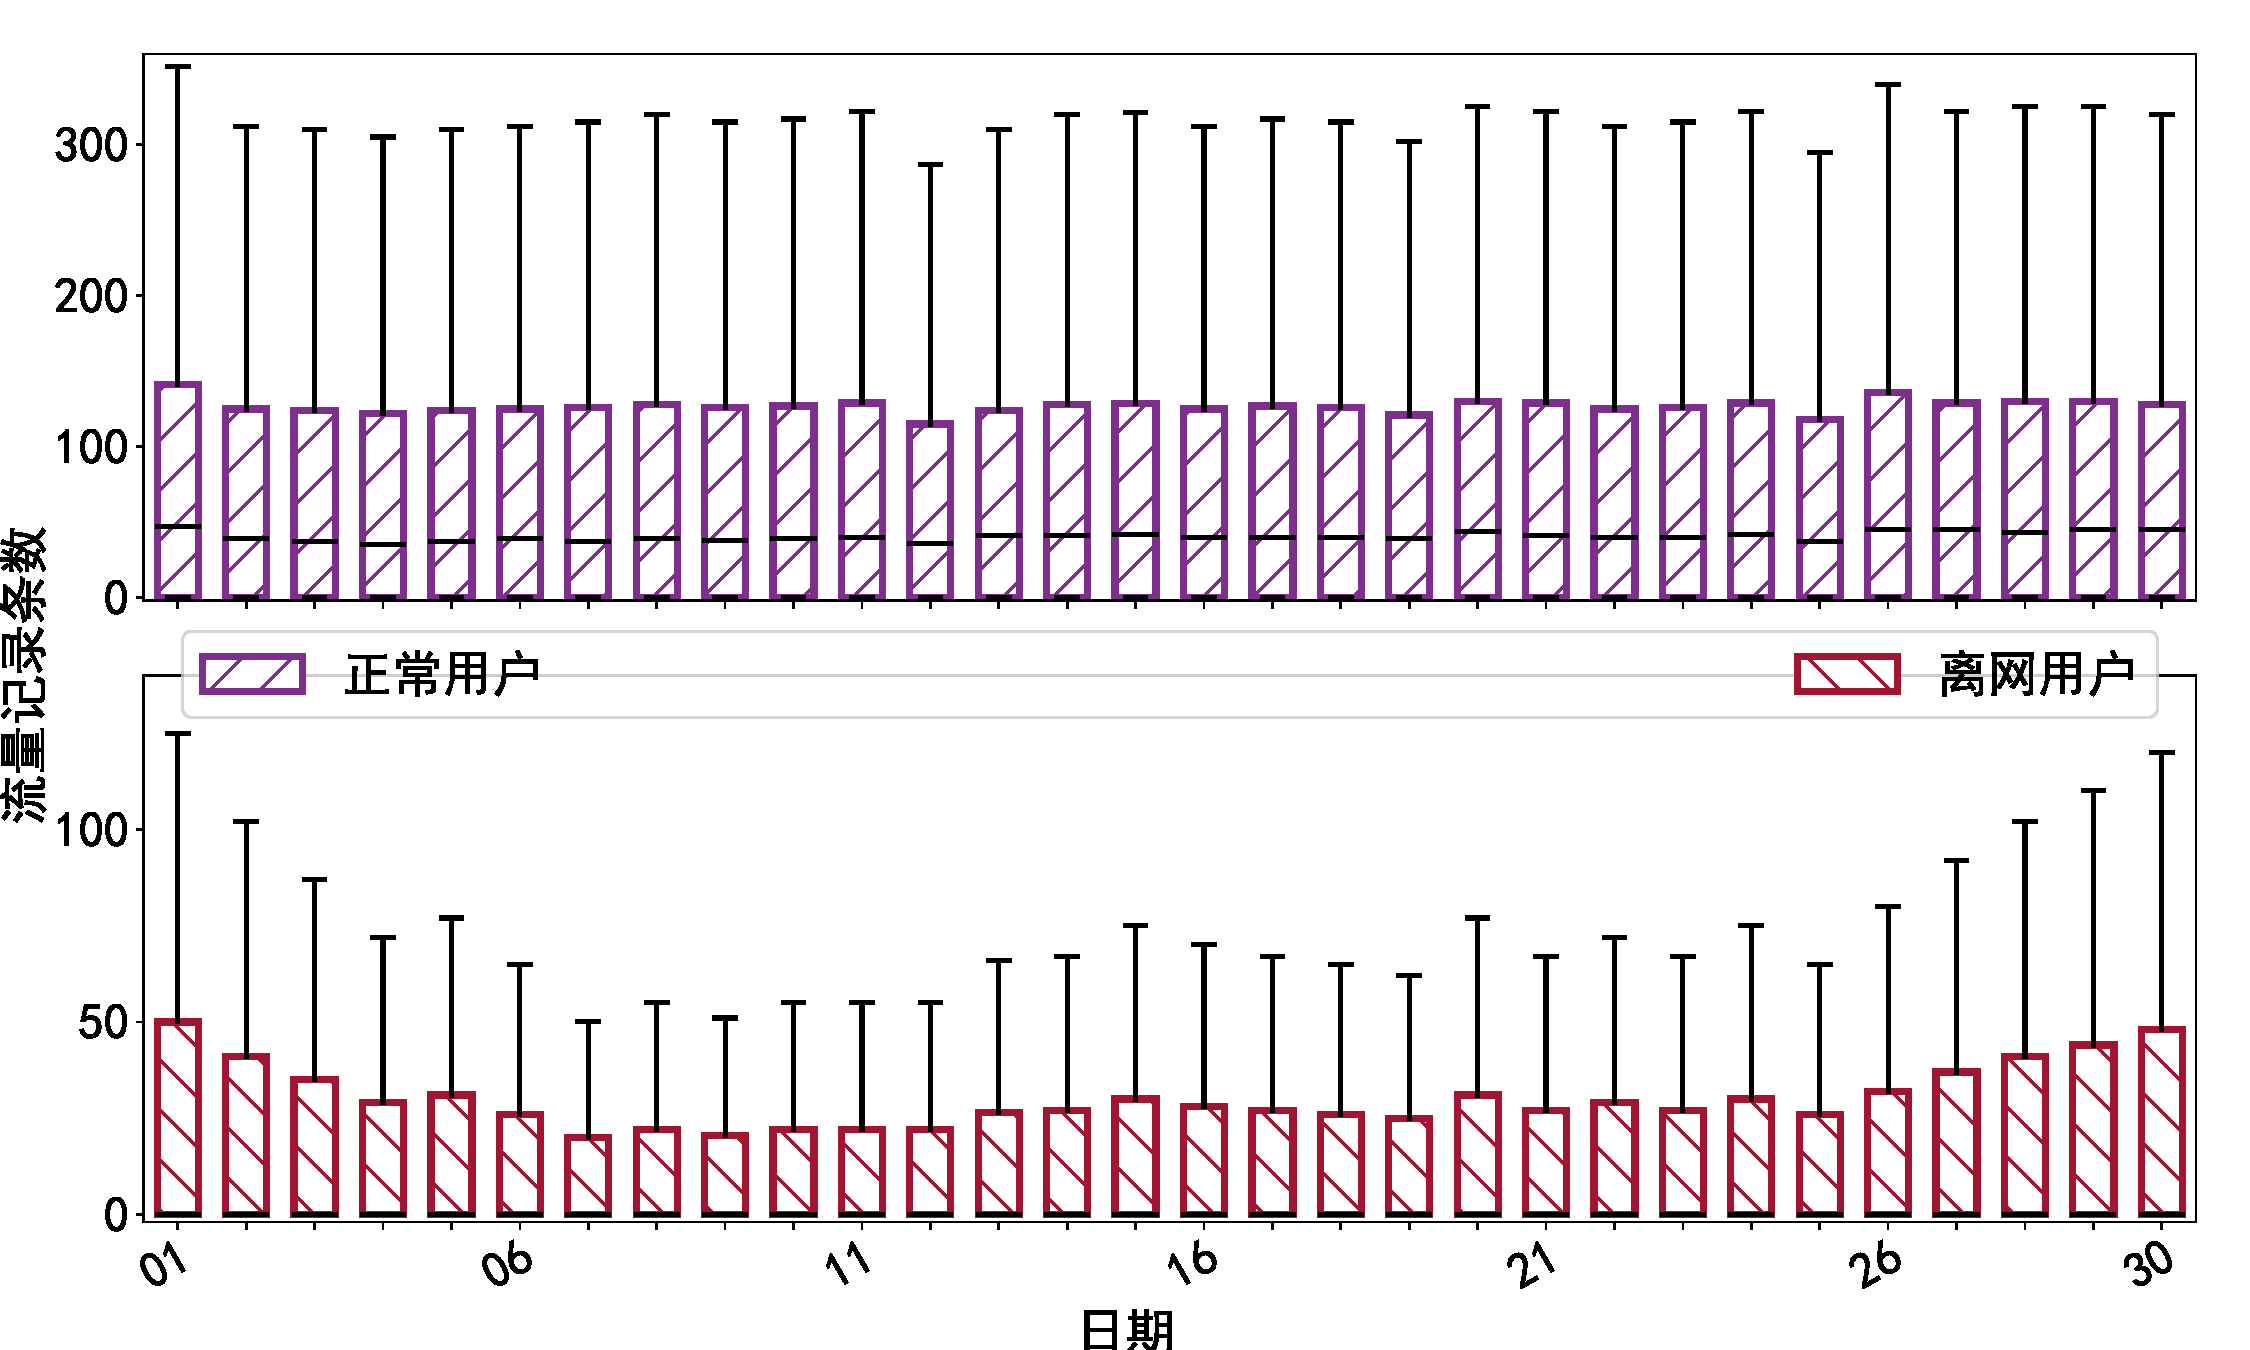
\includegraphics[width=1\textwidth]{Ms-Data_Traffic-Records-Date.pdf}
	\caption{互联网卡用户流量记录条数序列对比}
	\label{Fig:Traffic-Records-Date}
\end{figure}
图\ref{Fig:Traffic-Records-Date}展示了在一个月内的互联网卡用户的日产生流量记录条数的箱线图。本文可以从中观察到正常用户每日通常比离网用户都产生了更多数量的流量记录条数。更加重要的是,对于正常用户来说,时序行为的差异十分小,但是对于离网用户来说他们的流量使用行为显得更不稳定。这也意味着这种时间相关性能被加以利用用来区别这两种类型的用户。需要指出的是,除了每日流量记录,其他日粒度特征还包括上行流量值,下行流量值,上网时长,通话次数等,也都被提取成时序特征并且喂给了后续的学习模型。

\textbf{流量异常天数.}
\begin{figure}[hbt]
	\centering
	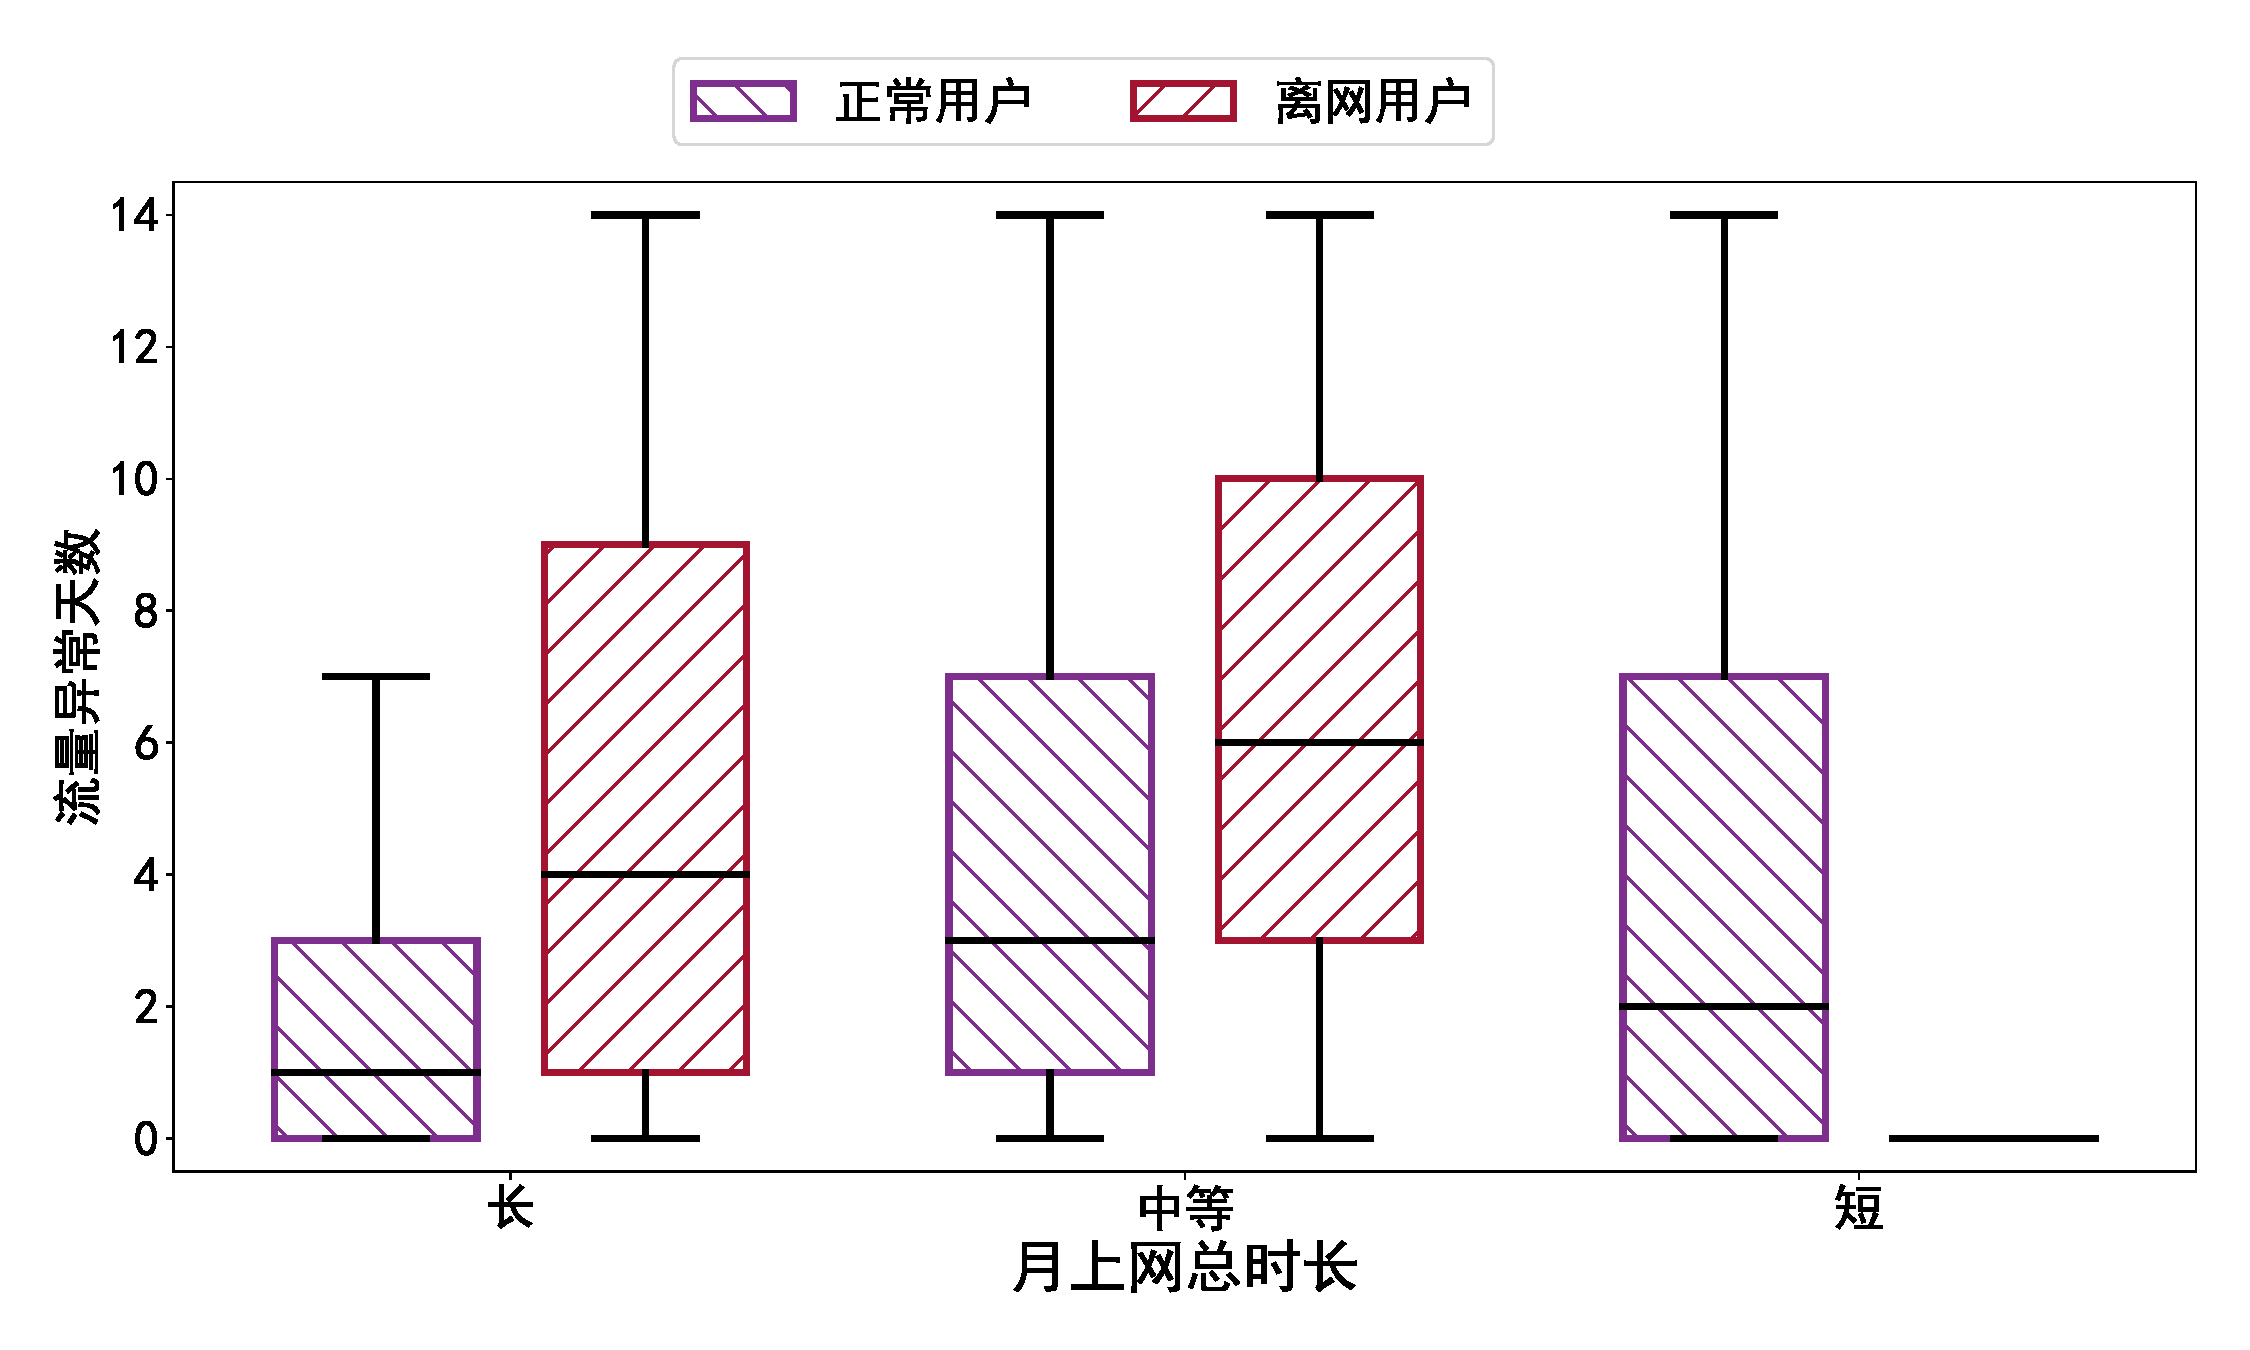
\includegraphics[width=1\textwidth]{Ms-Data_Traffic-Abnormal-Days.pdf}
	\caption{互联网卡用户流量异常天数对比}
	\label{Fig:Traffic-Abnormal-Days}
\end{figure}
除了分析互联网卡用户的流量统计特征,本文还检测了互联网卡用户在一个月内的哪些日期出现了流量异常行为,因为异常值往往表征着此用户表现同以往不同的行为,很有可能会趋向离网。明确来说,基于用户的日序列行为,本文对所有用户累加了使用特征值,包括上行流量值,下行流量值,上网时长和流量记录条数。因此,对每个序列特征来说,它都能被表征为$X=[B_{1}, B_{2}, ..., B_{i}, ...,B_{n}]$,其中$B_{i}$表示这个月内第i天的统计特征。为了获得更平稳的序列特征,本文对上述得到的序列特征计算了它们的一阶前向差分形式,用来$X^{'}=[F_{1}, F_{2}, ..., F_{i}, ...,F_{n-1}]$表示,可以用以下公式\eqref{Eq:Forward-Diff}计算。
\begin{equation}
	F_{i} = B_{i+1} - b_{i}
	\label{Eq:Forward-Diff}
\end{equation}
\\
然后,本文定义了异常值$E(X^{'})$,可以通过使用四分位距(IQR)加上以下公式\eqref{Eq:Abnormal}来判定。
\begin{equation}
	E(X^{'}) \textgreater Q_{u} + \gamma * IQR \lvert \rvert E(X^{'}) \textless Q_{l} * IQR
	\label{Eq:Abnormal}
\end{equation}
其中$IQR=Q_{u}-Q_{l}$,$\gamma = 1.5$。$Q_{u}$是上四分位值,显示只有1/4的观察值比它大,然后$Q_{l}$是下四分位值,这就意味着只有1/4的观察值比它小。因此,每天的流量行为是否是异常值可以通过计算用户序列特征前向差分值的异常值来判断。在图\ref{Fig:Traffic-Abnormal-Days}中,本文为正常用户和离网用户都描绘了月异常天数的箱线图。类似地,其中用户也被分成了三组,依据为在一个月内的总上网时长从高到低依次排序。具体来说,其中较高和中等的离网用户组明显拥有更多的异常天数,能够被利用来识别离网事件。但是对于使用较少的离网用户组来说,离网用户比正常用户有着更少的异常天数。这是合理的,因为他们有着稀疏的上网行为,这也导致了没有异常值产生。

%\subsection{本章小结}

%\section{基于自注意力机制的互联网卡用户离网预测模型设计}
\subsection{问题建模与模型描述}
\begin{figure}[hbt]
	\centering
	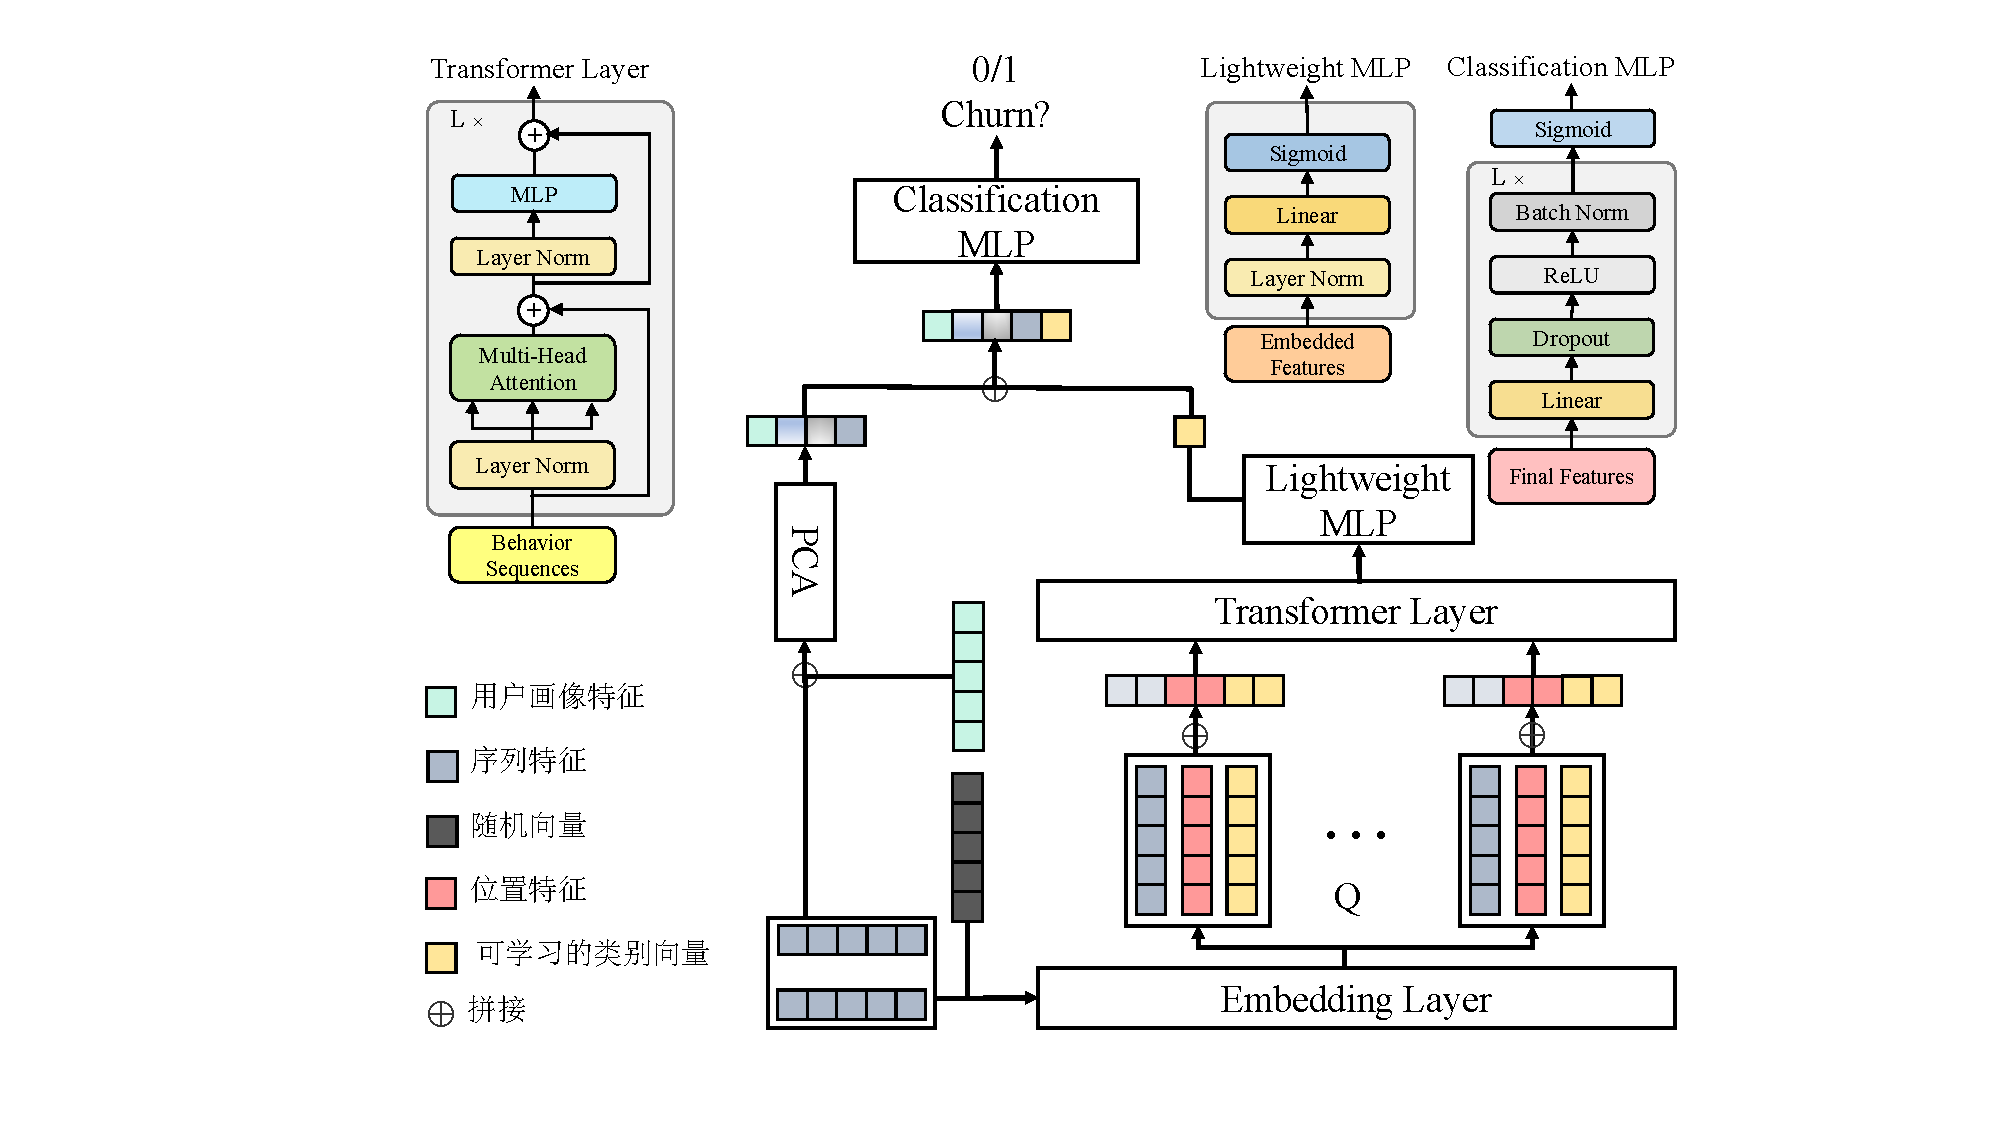
\includegraphics[width=1\textwidth]{Ms-ICCP_Architecture_2.pdf}
	\caption{互联网卡用户离网预测模型架构}
	\label{Fig:ICCP-Architecture}
\end{figure}
为了预测潜在的互联网卡离网用户,本文设计了一个可学习的模型架构:互联网卡离网预测Inter Card Churn Prediction(ICCP),其中包括基于主成分分析算法的特征降维算法,基于自注意力机制的编码算法,轻量级的多层感知机和分类的多层感知机的,如图\ref{Fig:ICCP-Architecture}所示。\\

\textbf{特征输入.}本文基于采集的数据构建了特征工程来提取用户属性和行为特征。对于这两种类型的特征,本文定义符号$\mathcal{P} \in \mathbb{R}^{1 \times M}$来表示画像特征矩阵,其中$M$表示所有静态特征的数量,定义符号$\mathcal{T} \in \mathbb{R}^{Q \times D}$来表示时序特征矩阵,其中$Q$是所有日粒度特征的数量,$D$是序列特征的长度。在为所有用户计算完这两类特征值后,它们将和离网标签一起被输入到可学习的模型来做监督学习。\\

\subsection{基于自注意力机制的编码算法}
\begin{algorithm}
	\caption{针对多重序列特征的嵌入变换算法}
	\label{ALG:Transformer-Encoding}
	\renewcommand{\algorithmicrequire}{\textbf{Input:}}
	\renewcommand{\algorithmicensure}{\textbf{Output:}}
	
	\begin{algorithmic}[1]
		\REQUIRE 时序特征$T^{(N*L)}$, 嵌入向量数量$Q$, 块长度$V$,块宽度$W$,嵌入向量大小$D$,变换块数量$L^\prime$
		\ENSURE 用户时序特征的编码向量$E^{(Q*D)}$
		\STATE 把时序特征$T^{(N*L)}$变形成块$B^{Q*(V*W)}$
		\STATE 训练一个全连接神经网络来编码块$B^{Q*(V*W)}$到块$B^{Q*D}$
		\STATE 随机初始化一个可学习的服从高斯分布的向量$X^D$   %\Comment{to represent the churn information}
		\STATE 随机初始化一个可训练的服从高斯分布的位置嵌入矩阵$M^{(Q+1)*D}$ %Comment{to learn the relative position between vectors in blocks} $B^{Q*D}$
		\STATE 拼接块$B^{Q*D}$, 向量$X^D$, 矩阵$M^{(Q+1)*D}$ 成$Z_0$  %Comment{as the input to transformer layer}
		\STATE 初始化$Q_i=W^Q_i*Z_0$,$K_i=W^K_i*Z_0$,$V_i=W^V_i*Z_0$, $i=1,...,3$
		\STATE 计算$Head_i=softmax(\frac{Q_i*K^T_i}{\sqrt{d_{k_i}}})V_i,i=1,...,3$
		\STATE 计算$MSA(Z_0)=Concatenate(Head_1,...,Head_3)*W^O$
		\STATE 计算$Z^\prime_l$ $=MSA(LN(Z_{l-1}))+Z_{l-1},l=1...L^\prime$
		\STATE 计算$Z_l$ $=MLP(LN(Z_{l-1}^\prime))+Z_{l-1}^\prime,l=1...L^\prime$
		\STATE 计算$E^{(Q*D)}$=$LN(Z^0_{L{^\prime}})$
		\STATE 返回$E^{(Q*D)}$		
		
	\end{algorithmic}
\end{algorithm}
为了捕捉潜在的时间关联性,矩阵$\mathcal{T}$和一个随机向量会首先被喂入到一个嵌入层(Embedding layer),它会输出一个固定维度大小的低维空间向量$Q$,在图\ref{Fig:ICCP-Architecture}可以看出,这个向量$Q$包含序列,位置和类别信息,并用不同的颜色标注了出来。然后这个向量$Q$被输入到了变形层(Transformer Layer),其中包括$L$个块,每个块中包含层归一化(LN),多头自注意力(MSA)和多层感知机(MLP),这相对应的函数可以被如下公式计算。
\begin{subequations}\label{Eq.(3-4)}
	\renewcommand{\theequation}{\theparentequation-\alph{equation}} % 定义编号方式
	\begin{align}
		&z_{0} = [s_{class}; \mathcal{T}^{1}; \mathcal{T}^{2}; ... ; \mathcal{T}^{\lvert D \rvert}; \mathcal{T}^{1}_{pos}; \mathcal{T}^{2}_{pos}; ...; \mathcal{T}^{D}_{pos} ], \label{Eq.(a)} \\
		&z_{l}^{'} = MSA(LN(z_{l-1})) + l-1, l=1...L \label{Eq.(b)} \\
		&z_{l} = MLP(LN(z_{l}^{'}))+z_{l}^{'}, \label{Eq.(c)} \\
		&y = LN(z_{L}^{0}), \label{Eq.(d)} 
	\end{align}
	\label{Eq:Transformer}
\end{subequations}
其中$z_{0}$是嵌入层的输出,$\mathcal{T}^{i}$表示第i个时序特征的信息,而$\mathcal{T}^{i}_{pos}$表示$\mathcal{T}^{i}$的位置嵌入信息。嵌入层和变形层的具体工作流程可见算法\ref{ALG:Transformer-Encoding}。在这之后,变形层的输出将被输入到轻量级的多层感知机(Lightweight MLP),其中包括层归一化,全连接层和Sigmoid层。然后轻量级的多层感知机将会输出一个离网概率值,后者将会被视为一个新特征注入到之后的分类多层感知机中。

\subsection{基于主成分分析算法的特征降维算法}
为了捕捉用户的画像信息,本文首先将用户画像特征和时序特征拼接成一个一维向量,比如说,$V_{i} = \{x_{1}, x_{2}, ..., x_{M+Q \times D}  \}$。然后这个向量将被输入到主成分分析算法这个组件。它会输出一个压缩向量$ W_{i}^{*} = \{ w_{1}, w_{2}, ..., w_{d^{'}} \} $, 其中$w_{d^{'}}$是新维度的大小。接着这个新向量和轻量级多层感知机的输出会被拼接,然后输入到最终的分类多层感知机中。需要特别指出的是,针对画像特征和时序特征的主成分分析算法能够在保持大多数特征成分的同时,比如最大限度地保留原始信息,这也能够减少用于分类的特征的复杂度,加速模型训练和收敛。具体的工作流可见算法\ref{ALG:PCA}。
\begin{algorithm}
	\caption{针对画像特征和时序特征的主成分分析}
	\label{ALG:PCA}
	\renewcommand{\algorithmicrequire}{\textbf{Input:}}
	\renewcommand{\algorithmicensure}{\textbf{Output:}}
	
	\begin{algorithmic}[1]
		\REQUIRE 用户画像特征$P$, 时序特征$T$, 信息阈值$I$
		
		\ENSURE 被信息阈值截断的关于用户特征的主成分$P_{c}$
		
		\STATE 初始化时序矩阵$t$为空
		\STATE 初始化信息权重$w$为0和主成分数量$n$为0
		\FOR{$i \gets 1\cdots Q$}
		\STATE $t \gets$ 拼接$t$和$T$的第$i_{th}$个时序特征
		\ENDFOR
		\STATE $P \gets$ 拼接t和P
		\STATE 并行对所有特征去中心化 $P_i =P_i - \frac{1}{M+Q*D} \sum_{j=1}^{M+Q*D} P_j$
		\STATE 计算特征的协方差矩阵 C=$\frac{1}{M+Q*D}PP^T$
		\STATE 计算特征值$\lambda$ 和 协方差矩阵$C$对应的特征向量$\vec v$
		\STATE 根据$\lambda$降序排列$\vec v$来得到矩阵$C'$
		\REPEAT
		\STATE $w=\frac{\sum_{i=1}^{n}\lambda_i}{\sum_{i=1}^{M+Q*D}\lambda_i}$
		\STATE $n\gets n+1$
		\UNTIL $w \textless I$
		\STATE 选择$C'$的前n行来得到变换矩阵A
		\STATE $P_c = AP$
		\STATE 返回 $P_c$
	\end{algorithmic}
\end{algorithm}

\subsection{基于多层感知机的分类器设计}
\textbf{模型训练.} 为了分类一个互联网卡用户是否是离网用户,本文将其建模成一个二分类的问题。本文通过使用分类多层感知机,其中包括L个块,每个块包含小批量归一化(Batch Norm),ReLU,Dropout和全连接层。为了训练这个模型,本文采用交叉熵作为损失函数,可以被以下公式\eqref{Eq:Cross-Entropy}所计算。
\begin{equation}
	\mathcal{L} = \frac{1}{N} \sum_{i}^{} -[y_{i} \cdot log(p_{i}) + (1-y{i}) \cdot log(1-p_{i})]
	\label{Eq:Cross-Entropy}
\end{equation}
其中$p_{i}$表示用户$i$离网概率值,而$y_{i} \in \{ 0, 1\}$是表示用户是否离网的标签,具体来说,$y_{i} = 1$代表此用户是一个离网用户,否则,$y_{i} = 0$此用户是一个正常用户。$N$表示所有训练样本的数量。

\subsection{本章小结}
\newpage

\section{关于离网预测模块的实验评估与结果分析}
\subsection{实验设置}
\begin{figure}[hbt]
	\centering
	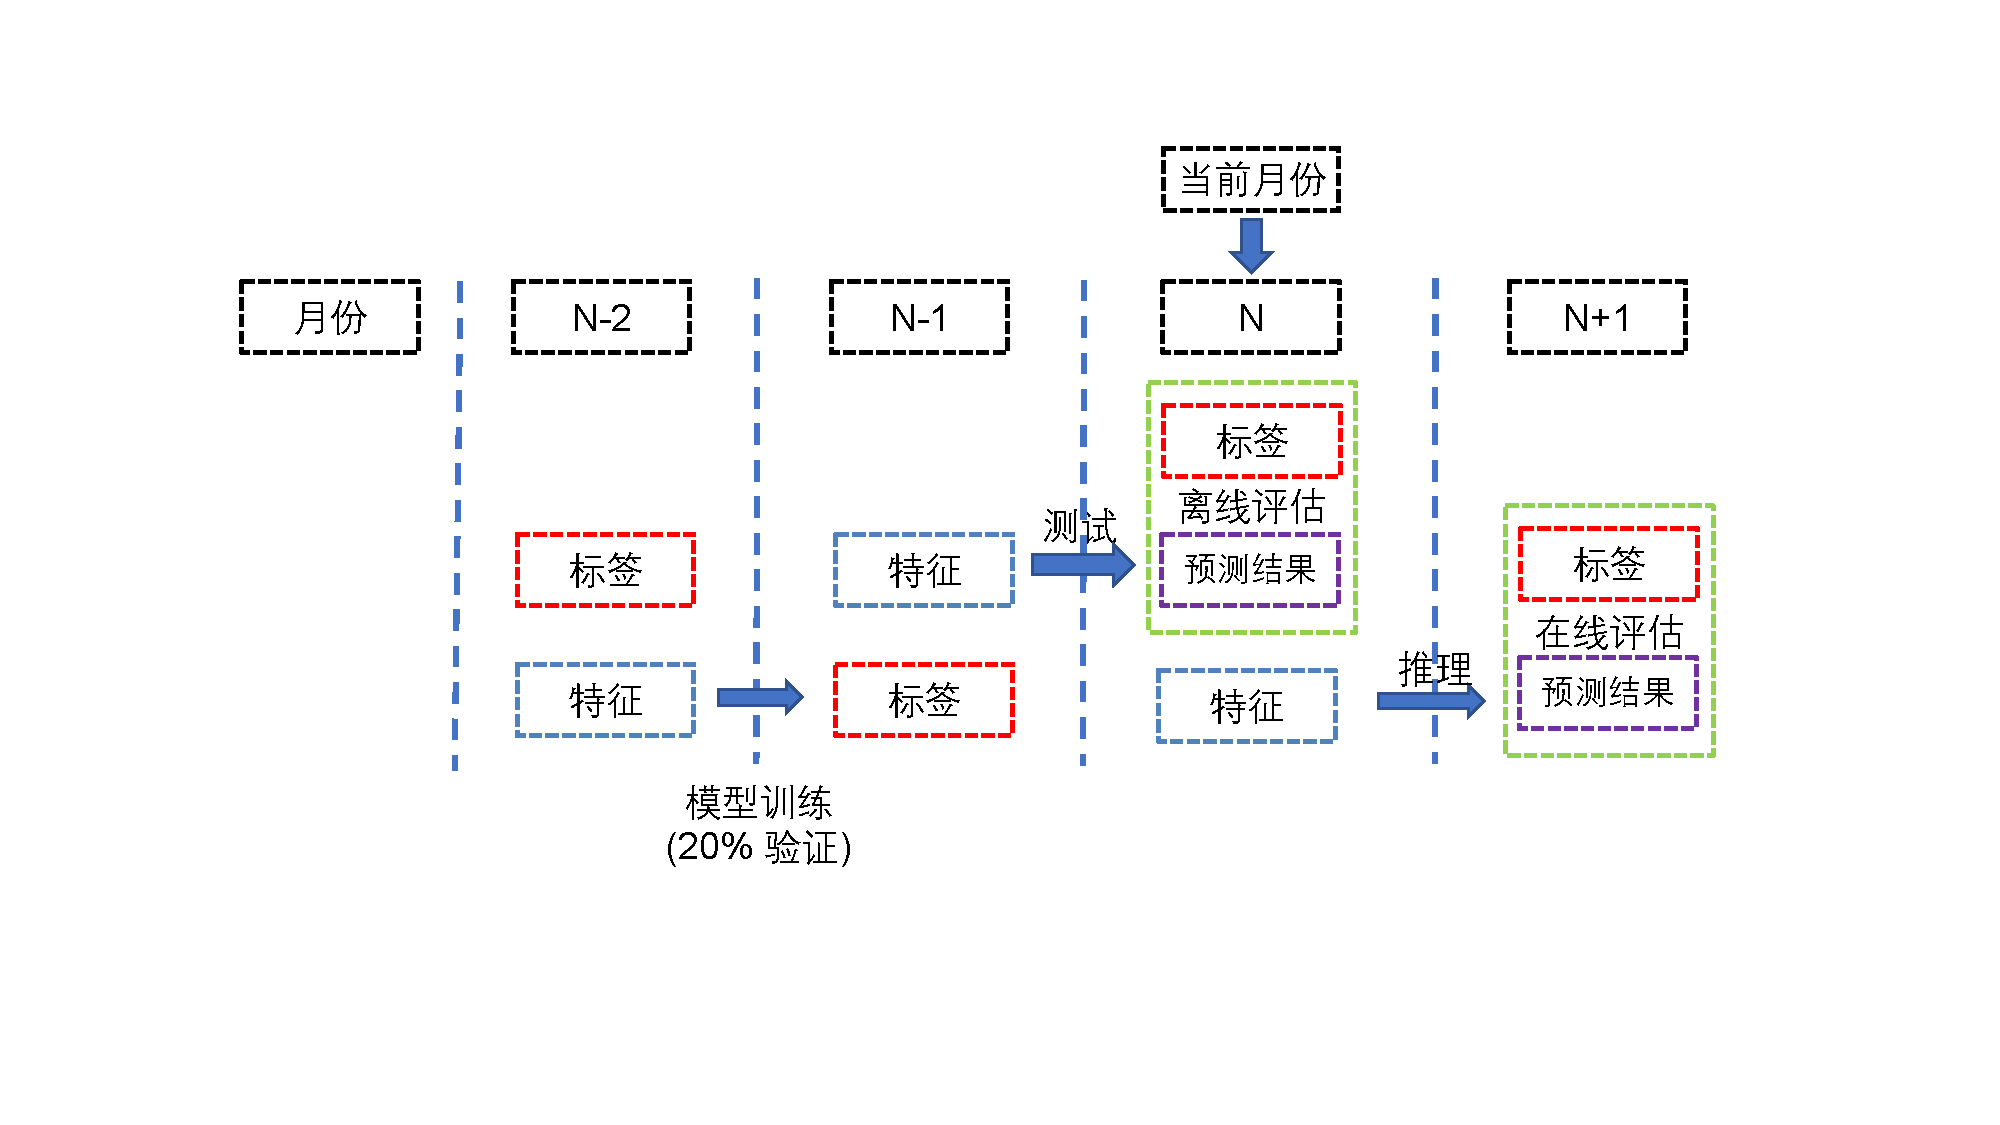
\includegraphics[width=1\textwidth]{Ms-ICCP_CP-Setting_v1_1.pdf}
	\caption{基于滑动窗口的离网预测实验设置}
	\label{Fig:CP-Setting}
\end{figure}
为了评估ICCP的性能,本文首先使用了某个运营商的互联网卡用户离网信息来标记离网用户,比如,如果一个互联网卡用户双停超过两个礼拜并且没有复机行为,那该用户就会被标记为离网用户。图\ref{ALG:PCA}展示了在不同月份基于滑动窗口的训练和预测实验设置。需要特别指出的是,假设当前月份是$N$月,本文首先会使用$N-1月$的用户离网信息来标记拥有$N-2$月特征的用户,然后用相同的方法使用$N$月的用户离网信息来标记拥有$N-1$月特征的用户。然后,我们使用拥有$N-2$月特征的用户和$N-1$月的标签来训练ICCP,其中20\%的数据样本用于验证。接着,本文使用拥有$N-1$月特征的用户和$N$月的标签来测试ICCP的离线性能。最后,依赖于上述机制,本文把$N$月无标签的用户特征数据输入到ICCP中,就可以得到下一个月的互联网卡离网用户名单,并且可以在下月评估ICCP的在线真实性能。综上所述,本文利用滑动窗口机制,通过将窗口从上个月移动到当前月实现用户的特征捕捉,然后使用ICCP模型来预测下月的潜在离网用户。\\
对于特征工程和性能评估,本文使用了横跨五个月采集的数据,分别是2020年的5月、6月,11月、12月和2021年的1月。其中2020年的6月、12月和2021年的1月的数据分别用来标注2020年5月、11月和12月互联网卡用户(是离网用户还是正常用户)。然后,本文使用相应的数据样本来进行离网预测模型的训练和测试。由于系统资源的限制,本文随机挑选了50万的互联网卡用户作为一个月的数据样本,其中在2020年5月有493251个正常用户和6749个离网用户。此外,对于2020年11月和12月的互联网卡用户而言,则有871049个正常用户和73289个离网用户。因此,本文在2020年5月、6月、11月和12月的500000个个944338个数据样本上构建了实验,其中80\%的样本用于训练,剩下20\%的样本用于测试。
\subsubsection{基准模型}
为了显示本文提出的ICCP模型的优越性,本文设计和实现了一下可以比较的分类基准模型 ,包括机器学习和深度学习模型。值得注意的是,虽然这些算法在科研文献中被广泛采纳用来解决分类问题,在其中却没有解决互联网卡离网分类和预测的。另外,为了保证比较的公平性,所有的基准模型的特征输入都与ICCP保持一致。
\begin{itemize}
	\item \textbf{随机森林(RF)}:是一种被广泛采纳用来分类问题的基于决策树的传统机器学习算法。
	\item \textbf{轻量梯度提升机(LGBM)}:是一种基于决策树算法的分布式梯度提升机器学习框架。这种机器学习提供了高效率并行训练,低内存消耗,更高准确率和大量数据的快速处理。
	\item \textbf{长短期记忆网络(LSTM)}:是深度学习领域内的一种循环神经网络架构(RNN)。它能很好地捕捉序列数据中的短期时间相关性。
	\item \textbf{多层感知机(MLP)}:是人工神经网络中的一种基础模型。它利用反向传播机制来进行模型训练。多层感知机架构是由包含全连接层,批量归一化(BN)层,ReLU层,Dropout层的块堆积而成的。
	\item \textbf{残差前馈神经网络(ResMLP)}:是一种基于残差连接的神经网络架构。其中包括一个隐层前馈神经网络和一个线性的残差连接。和多层感知机相比,残差前馈神经网络是一种拥有三个块层的更简单的残差网络架构。在本文离网预测场景当中,我们在每三个块层中添加了一个残差连接用来解决反向传播过程当中的梯度消失问题。
\end{itemize}


\subsubsection{评估指标}
对于离网预测问题来说,基于以下这四个基础测试结果,分别是真阳性样本(TP),假阳性样本(FP),真阴性样本(TN),假阴性样本(FN),我们采用了一下5个评价指标来评估相应性能。
\begin{itemize}
	\item \textbf{精准率(Precision)}:指的是一个被预测为离网的用户被正确预测的概率,具体公式为,$\frac{TP}{TP+FP}$。
	\item \textbf{召回率(Recall)}:指的是在真实标签中所有离网用户被正确预测的概率,具体公式为,$\frac{TP}{TP+FN}$。
	\item \textbf{F1分数(F1-Score)}:被定义为精准率和召回率的调和平均数,具体公式为,$2 \times \frac{Precision \times Recall}{Precision + Recall}$。
	\item \textbf{接收者操作特征曲线下面积(AUC)}:被定义为随机挑选一个正样本和负样本,正样本能排在负样本之前的概率。该评价指标用来判断模型是否擅长分类。具体公式为,$\frac{\sum_{i \in positiveClass}rank_{i} - \frac{M(M+1)}{2}}{M \times N}$,其中M和N分别表示正样本和负样本的数量。
	\item \textbf{精准率-召回率曲线下面积(PR-AUC)}:被定义在同一张图中根据不同阈值同时画出的精准率-召回率曲线下的面积。这项评价指标等同于根据不同阈值计算的召回率和精准率的平均乘积累加和。具体公式为,$\sum_{k=1}^{N}P(k) \Delta
	 R(k)$。
\end{itemize}

\subsection{用户离网预测模型性能评估}
\subsubsection{系统总体性能}
\begin{figure}[hbt]
	\centering
	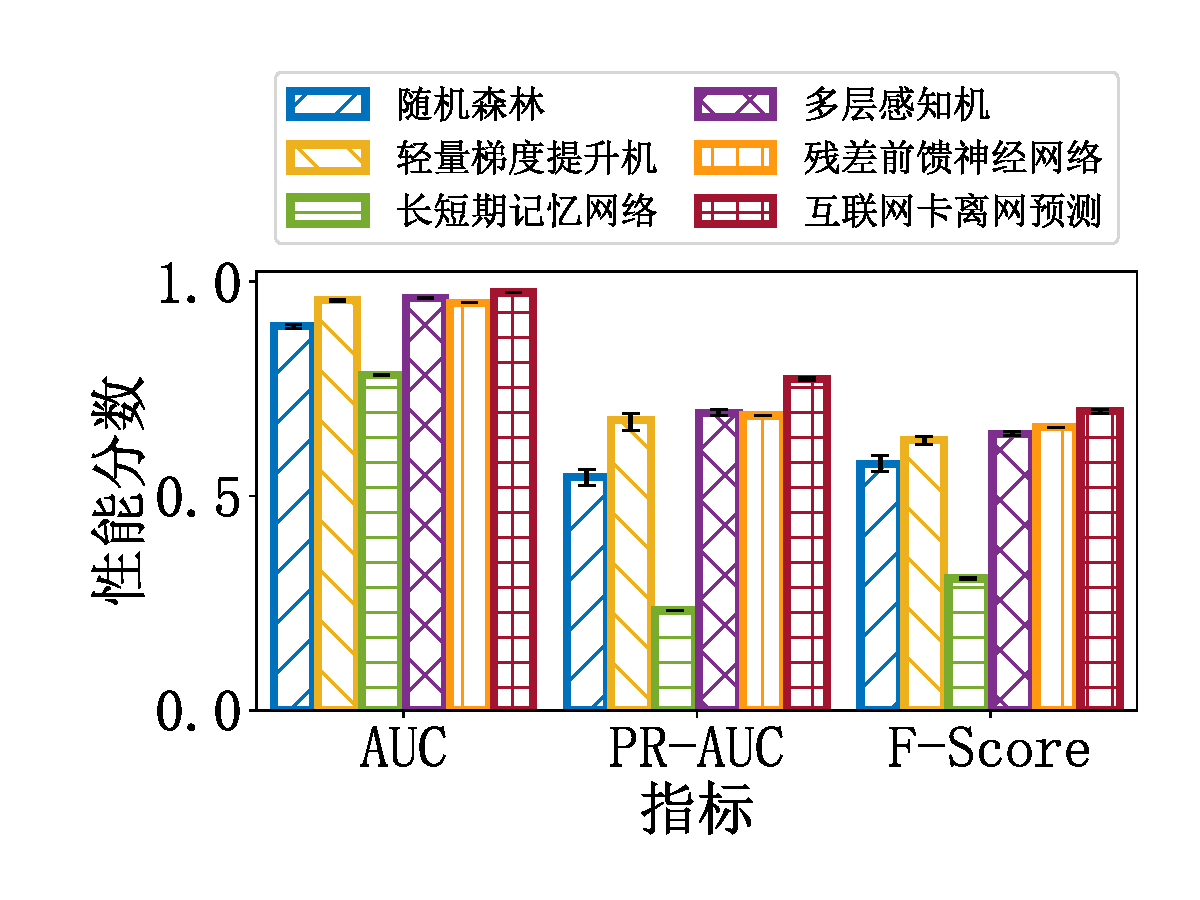
\includegraphics[width=1\textwidth]{Ms-ICCP_Model-Performance-Comparison.pdf}
	\caption{离网预测性能对比}
	\label{Fig:Model-Performance-Comparison}
\end{figure}
本文首先通过与基线模型的对比来检验本文提出的模型ICCP的系统总体性能。在把所有数据平均分成5组(比如,k折交叉验证中方法k=5)来计算性能的平均值和上下界,图\ref{Fig:Model-Performance-Comparison}展示了不同分类模型的性能表现。本文可以做出以下推断:首先就AUC,PR-AUC和F1分数而言,本文提出的ICCP模型可以显著超越基线模型。具体来说,随机森林,轻量梯度提升机,长短期记忆网络,多层感知机和残差前馈神经网络的平均PR-AUC分数分别为0.54, 0.67, 0.23, 0.69和0.68,在另一方面,ICCP的平均PR-AUC分数为0.77。其次,与其他基准预测模型相对比而言,长短期记忆网络表现出了最差的性能,这是因为长短期记忆网络只能捕捉时序特征而忽略了静态画像特征。第三,通过比较随机森林、轻量梯度提升机和长短期记忆网络、多层感知机和残差前馈神经网络,本文可以发现深度学习模型展示了提高互联网卡用户离网预测准确率的潜力。这里面的主要原因为深度学习模型可以通过利用多维度特征学习隐含信息表示。需要指出的是,本文也测试了其他机器学习模型,包括决策树,支持向量机和梯度提升树等,最终本文选取了表现性能最好的随机森林和轻量梯度提升机作为机器学习模型的代表。

\subsubsection{Top-U用户的性能.}
\begin{figure}[hbt]
	\centering
	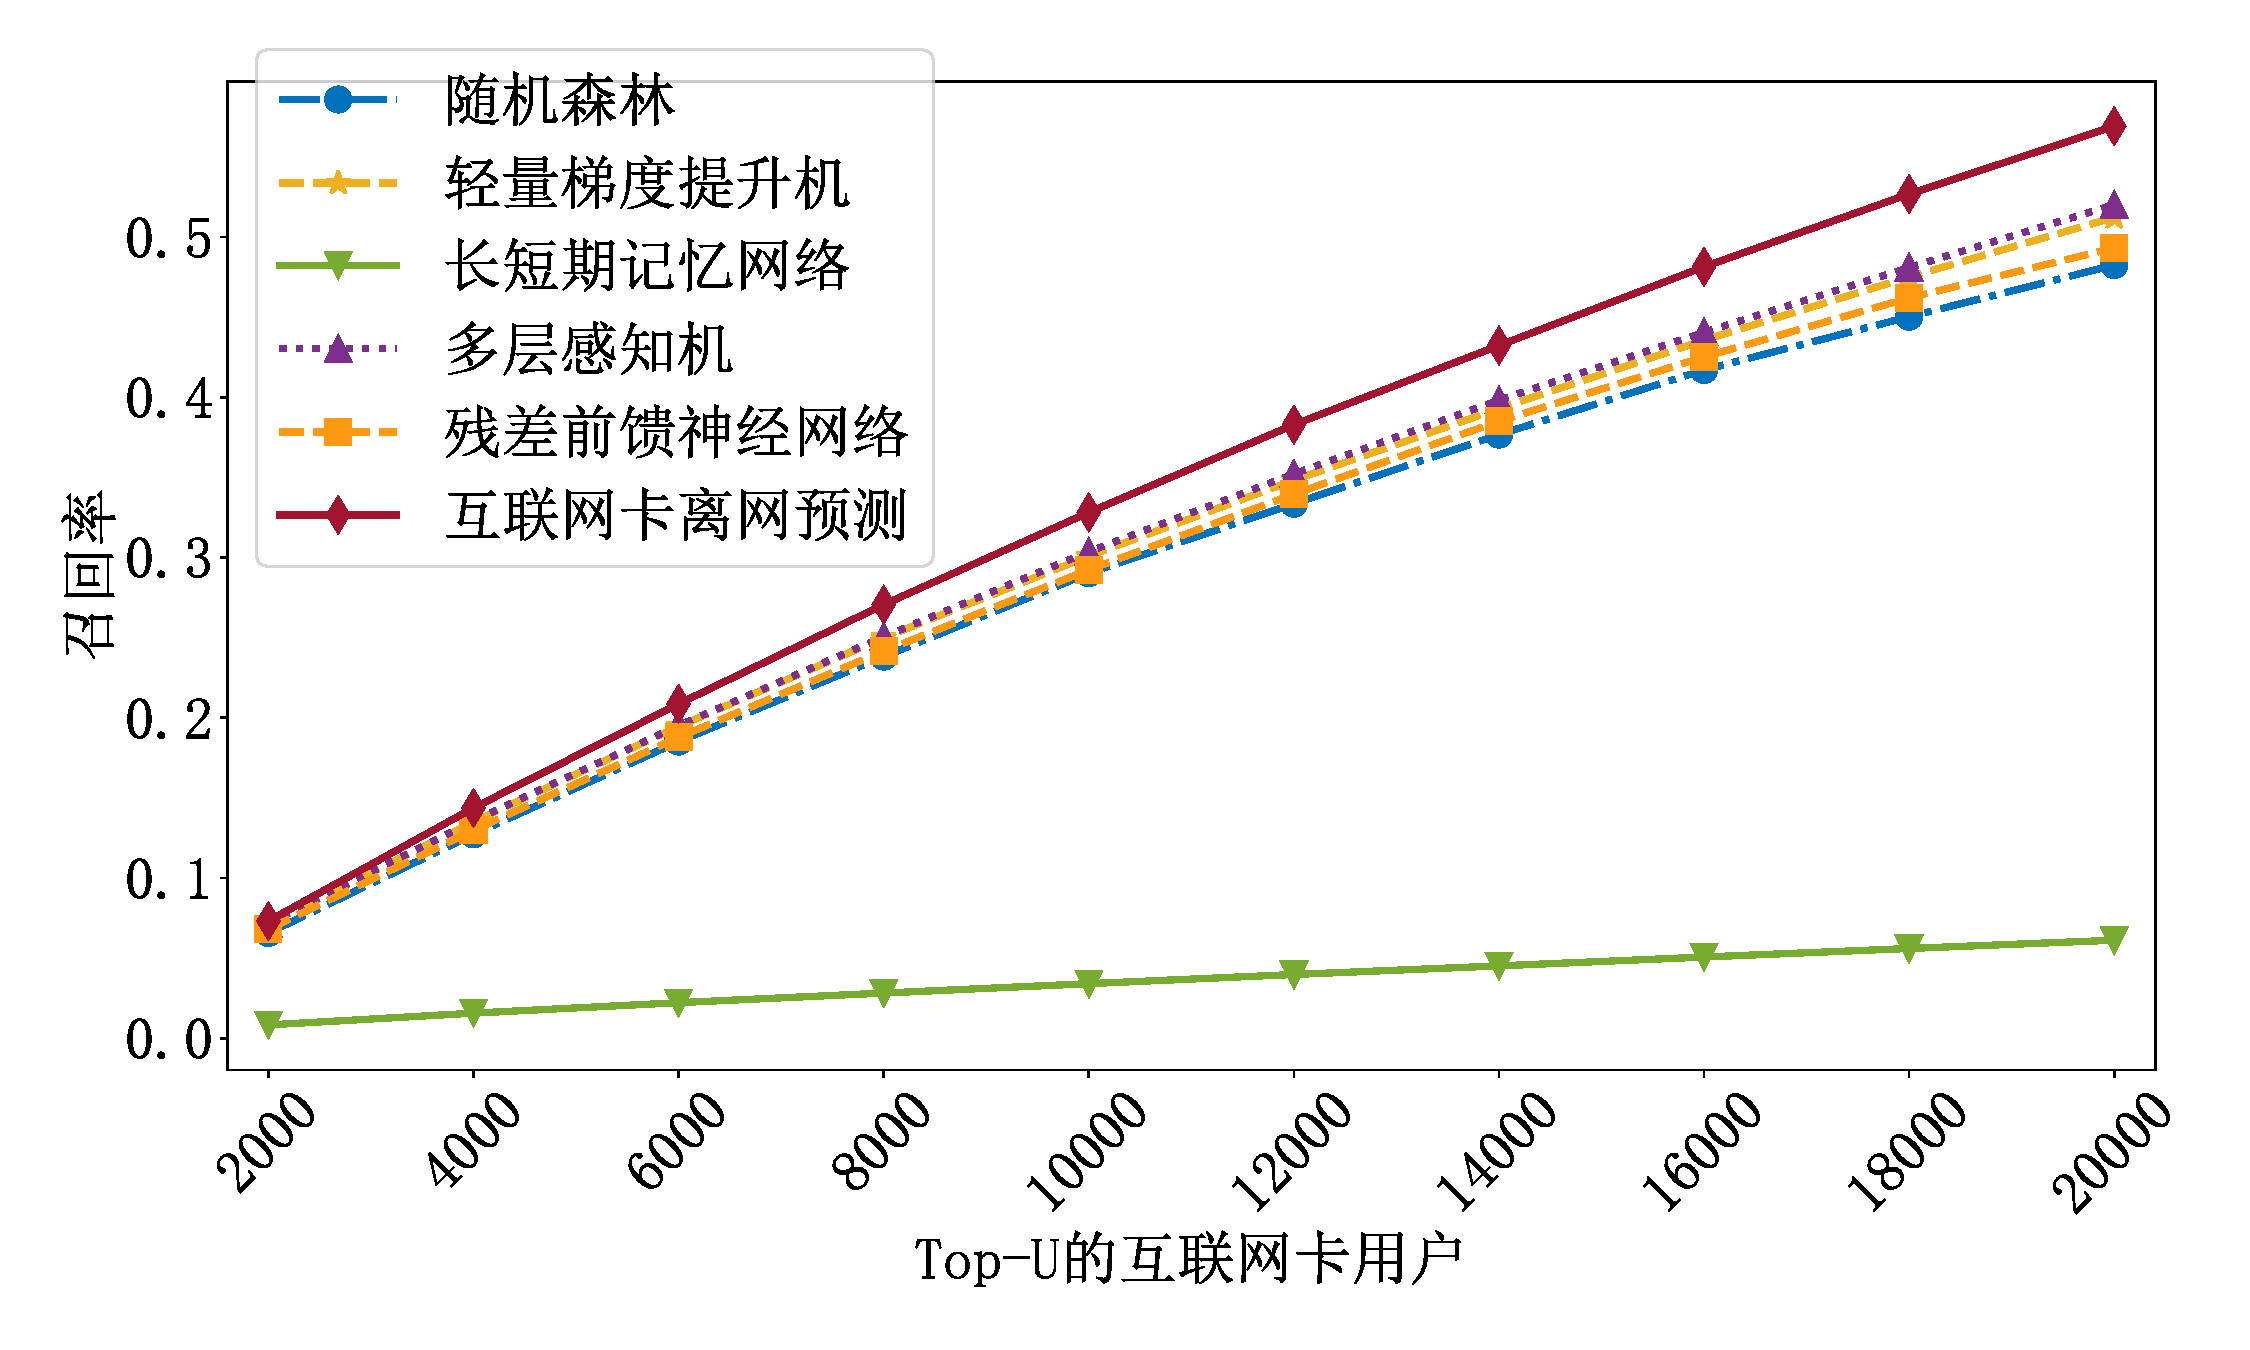
\includegraphics[width=1\textwidth]{Ms-ICCP_TopU-Recall.pdf}
	\caption{Top-U用户的召回率对比}
	\label{Fig:TopU-Recall}
\end{figure}

\begin{figure}[hbt]
	\centering
	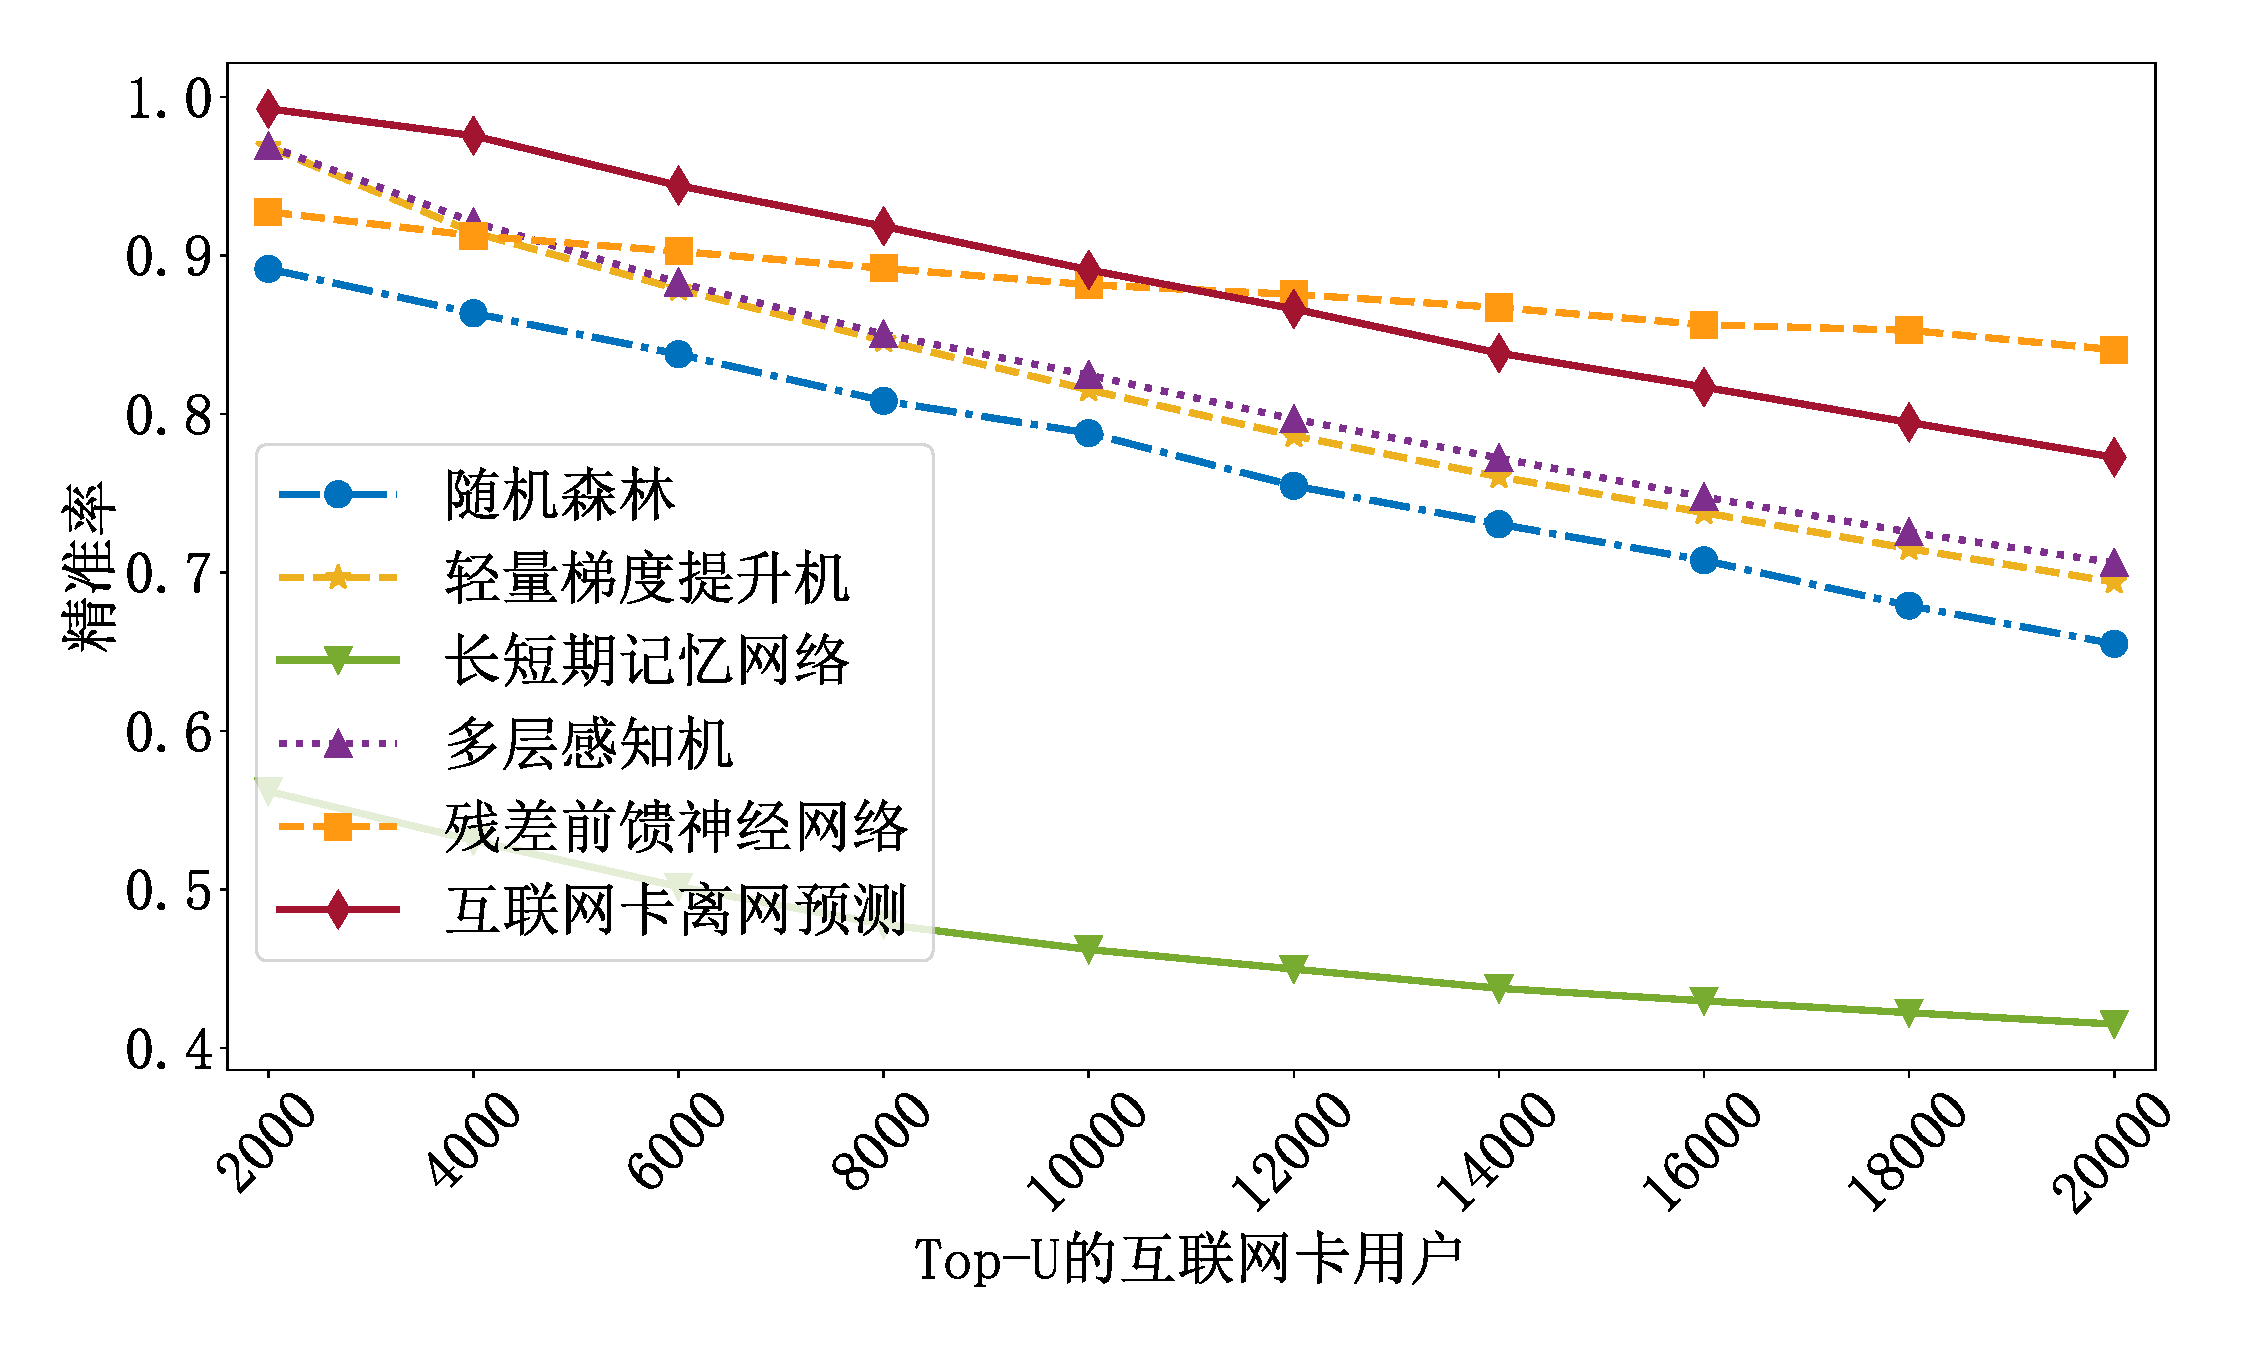
\includegraphics[width=1\textwidth]{Ms-ICCP_TopU-Precision.pdf}
	\caption{Top-U用户的精准率对比}
	\label{Fig:TopU-Precision}
\end{figure}

\begin{figure}[hbt]
	\centering
	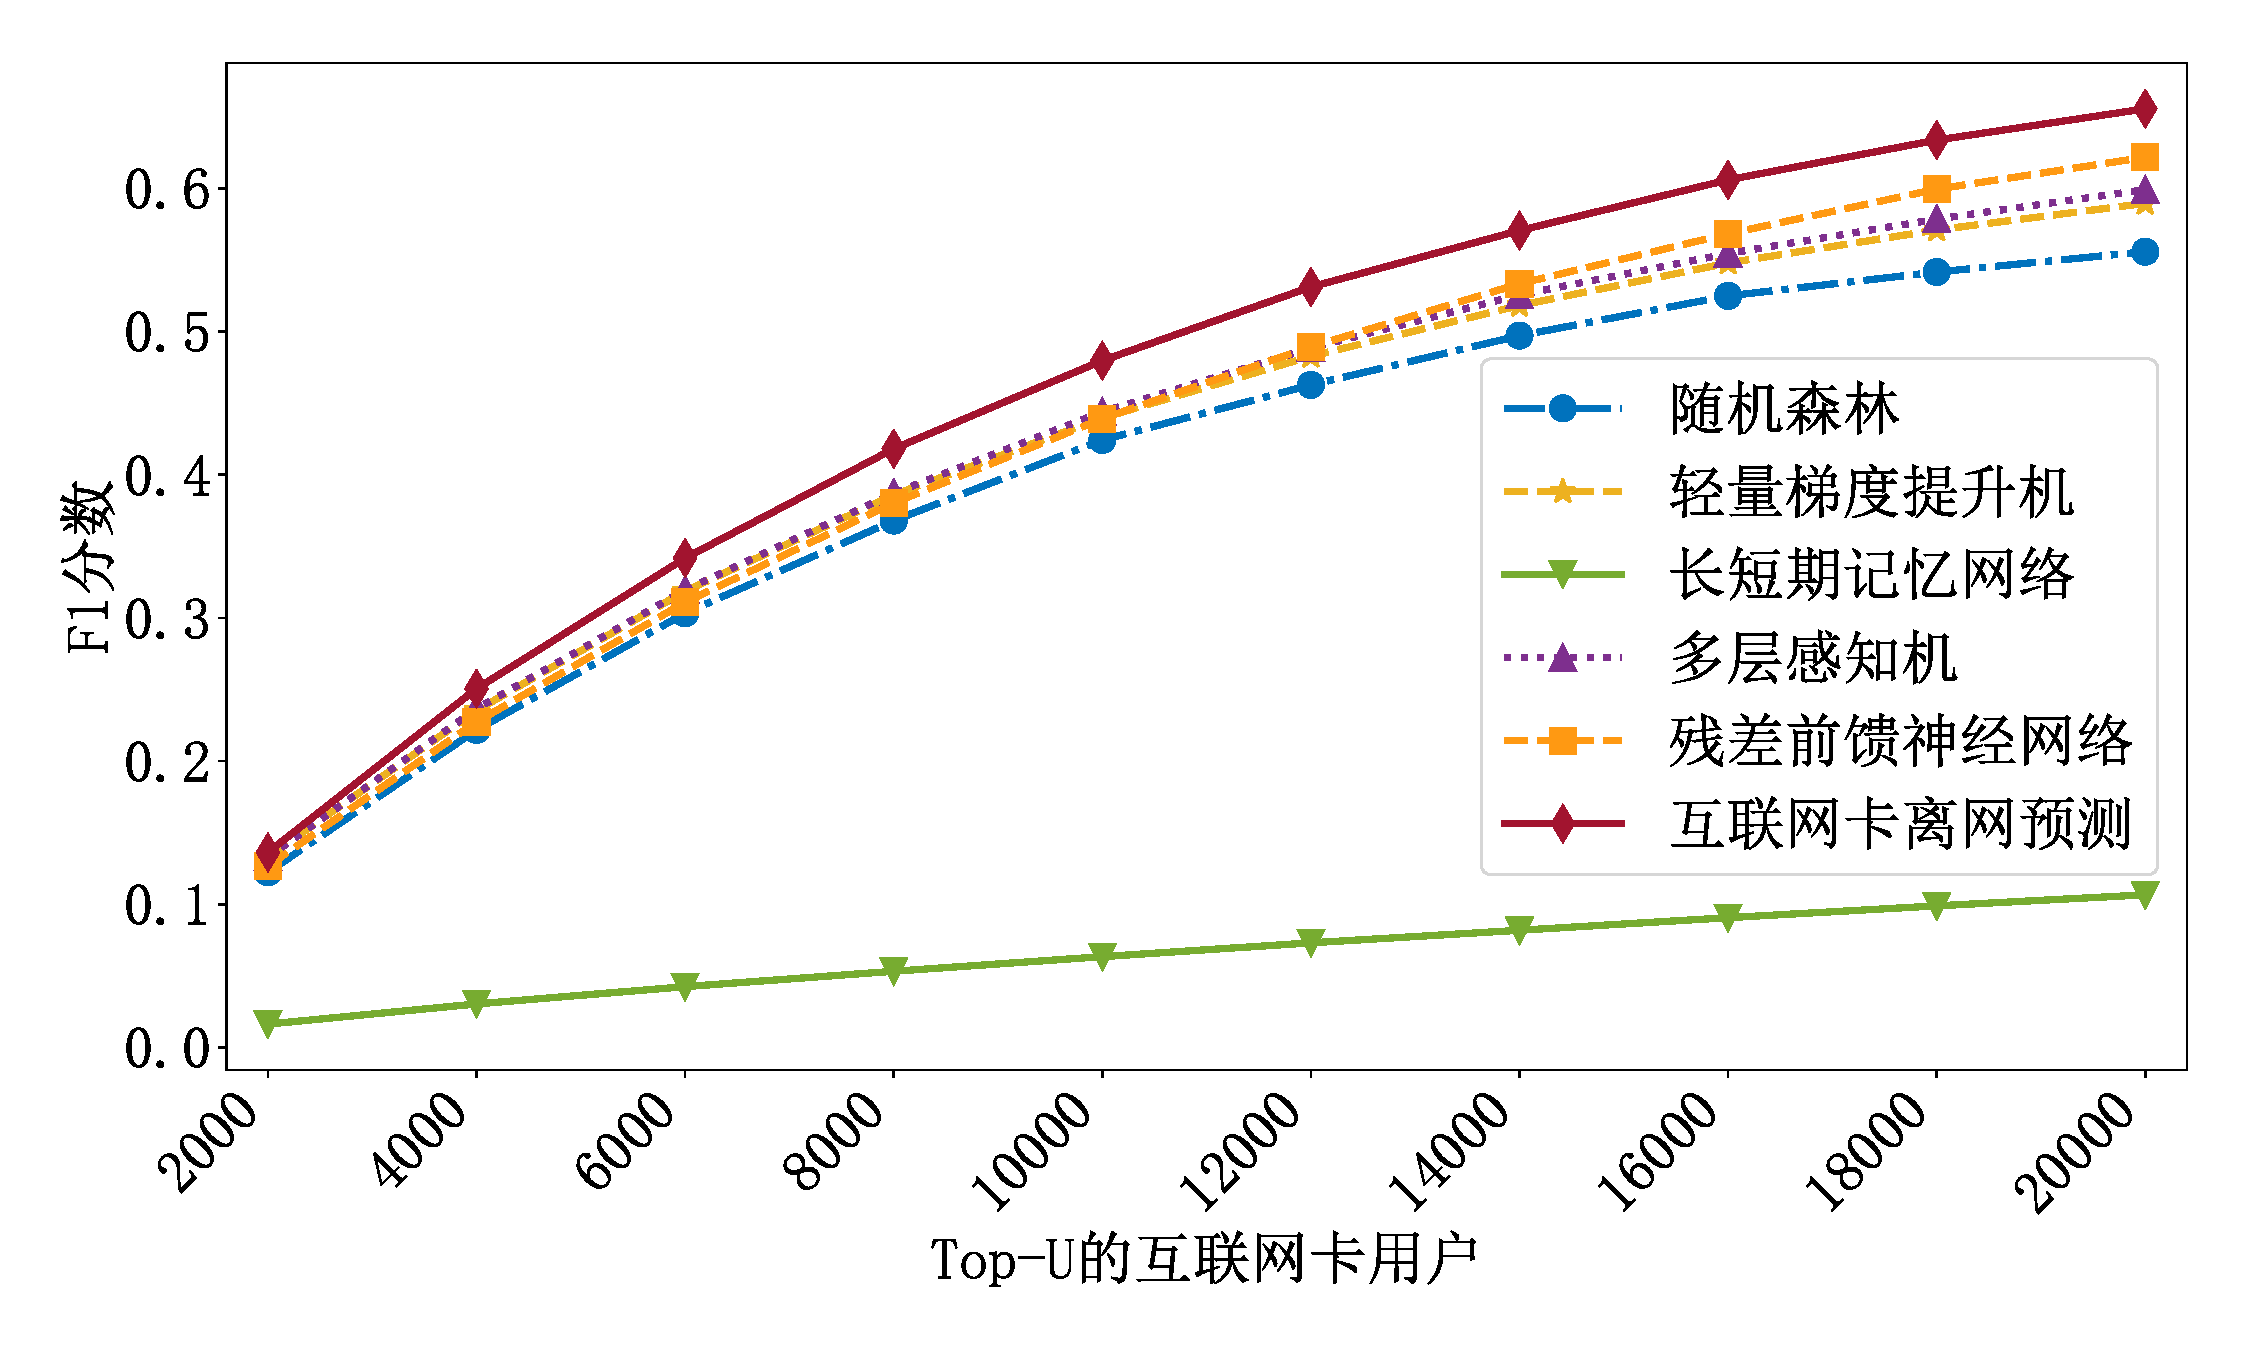
\includegraphics[width=1\textwidth]{Ms-ICCP_TopU-F1Score.pdf}
	\caption{Top-U用户的F1分数对比}
	\label{Fig:TopU-F1Score}
\end{figure}
为了进一步评估离网预测模型的性能,我们测试了Top-U个互联网卡用户的模型表现。需要特别指出的是,整个预测系统将会产生Top-U个互联网卡用户的名单,其中是最有可能在下个月离网的用户,接着我们评估了他们的预测性能。这个Top-U用户性能的评价指标可以作为运营商做决策的重要参考。图\ref{Fig:TopU-Precision},图\ref{Fig:TopU-Recall}和图\ref{Fig:TopU-F1Score}分别展示了Top-U用户的精准率(Precision@U)、召回率(Recall@U)和F1分数(F1-Score@U)。其中用户范围是从前2000个一直到前20000个。本文做出了以下的主要观察。\\
首先,在Top-U用户的设置下,我们提出的ICCP模型能在Recall@U和F1-Score@U这两项指标上明显超过其他基准模型。举例来说,ICCP的Precision@20000,Rcall@20000,F1-Scoren@20000分数为$\{ 0.77, 0.60, 0.65\}$,与此同时残差前馈神经网络,多层感知机,轻量梯度提升机,长短期记忆网络和随机森林的对应分数分别为$\{ 0.84, 0.49, 0.62\}$,$\{ 0.70, 0.52, 0.53\}$,$\{ 0.69, 0.51, 0.59\}$,$\{ 0.65, 0.48, 0.55\}$和$\{ 0.41, 0.06, 0.11\}$。第二,对于Precision@U和Recall@U这两个评价指标而言,随着用户U数量的增加,精准率是逐渐下降的,与此同时,召回率却是逐渐上升的。这是合理的,因为在用户U很少的情况下,这些被识别出来的预离网用户往往拥有更高的可能性离网运营商,这导致了精确率较高,但在另一方面,由于用户基数较少,也导致召回率较低。第三,随着用户U的增加,Precision@U的下降趋势和Recall@U的增长逐渐放缓的趋势共同说明了随着用户U的增加,从中识别出离网用户变得越来越困难。此外,当Top用户数量大于12000时,残差前馈神经网络的精确率要高于其他方法是因为被添加到残差前馈神经网络中的残差连接结构。这个结构大大改善了在反向传播中的梯度消失问题,同时也使得残差前馈神经网络在预测Top-U用户时更加平衡,下降趋势也更加平缓。但是,本文提出的ICCP模型在F1分数这个综合指标上能超过残差前馈神经网络这个基线模型,是因为后者在召回率分数上增长缓慢。







\subsection{参数影响}
在保证了预测性能后,我们进一步探讨了用户性别、年龄、App使用情况、套餐选择等用户属性参数对预测性能的影响。
\subsubsection{性别参数的影响}
%\textbf{性别参数的影响.}
我们将用户样本分为男性和女性两个子集,采用k = 5的k折交叉验证方法分别评估模型性能。
\begin{figure}[hbt]
	\centering
	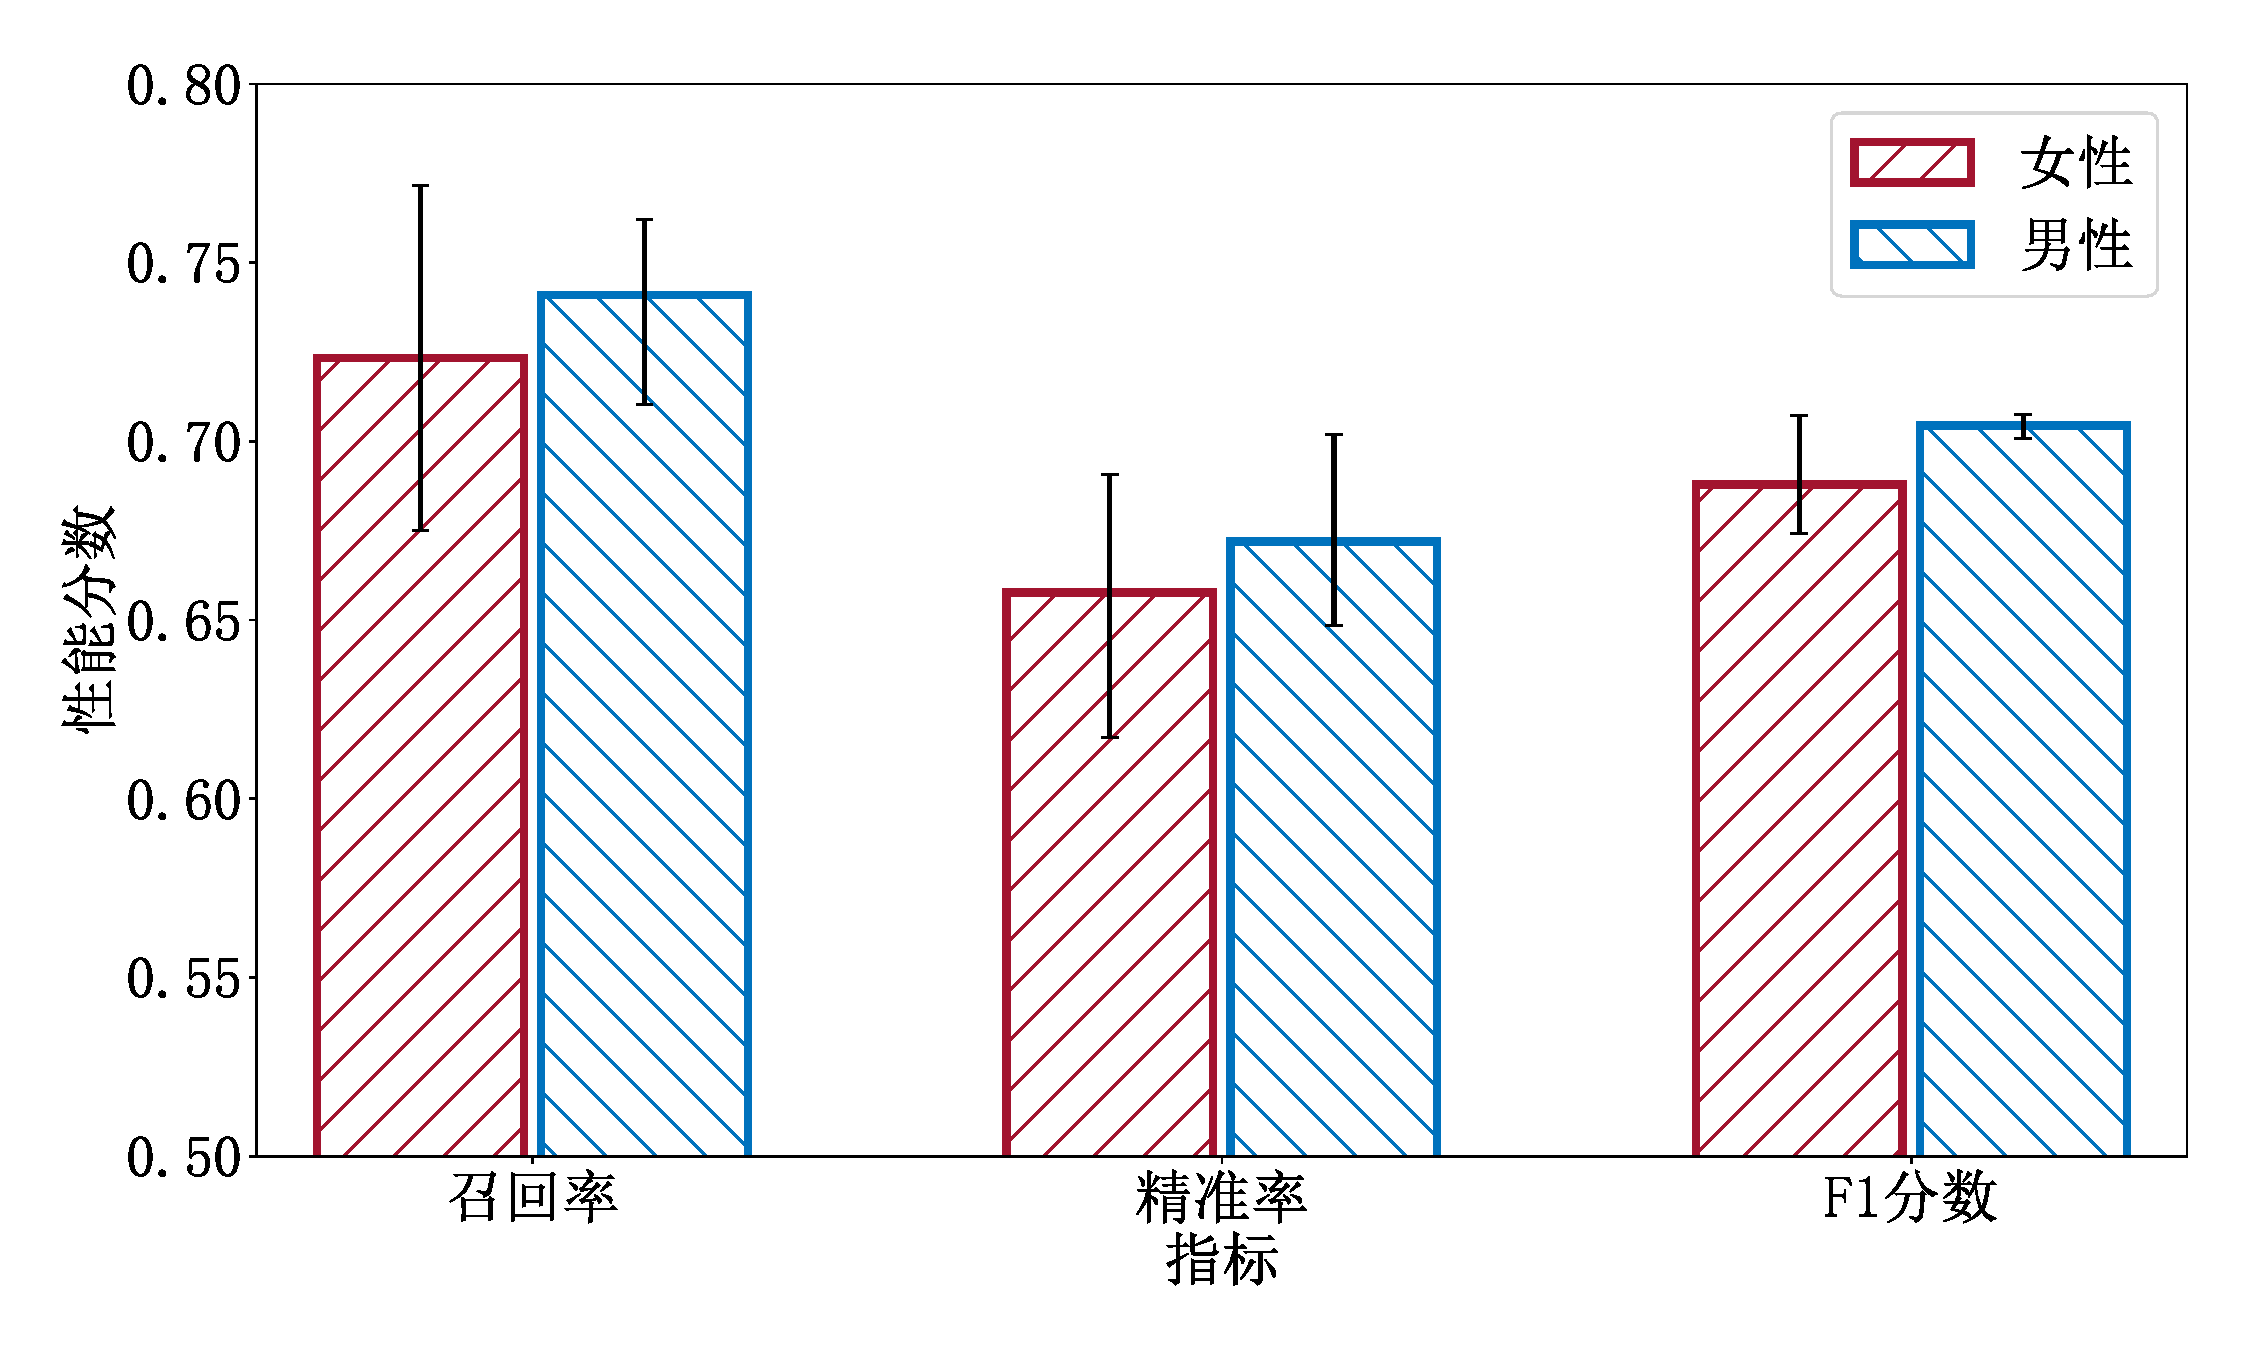
\includegraphics[width=1\textwidth]{Ms-ICCP_Impact-Gender.pdf}
	\caption{性别参数的影响}
	\label{Fig:Ms-ICCP_Impact-Gender}
\end{figure}
图\ref{Fig:Ms-ICCP_Impact-Gender}绘制了平均性能度量分数,其中男性和女性用户都有错误条用来,显示模型性能的上下界。本文可以得到以下结论:ICCP对男性和女性均是有效的,他们的指标得分非常相似,并且与系统的整体性能相当。如,对于召回率、精准率和F1分数的指标,女性用户可以分别获得0.72、0.66和0.69的平均分,而男性用户可以分别获得0.74、0.67和0.71的平均分。另一方面,我们可以发现男性的指标得分略大于女性用户,这与男性用户比女性用户有更多的流量消耗行为是一致的。可以解释为,流量消费行为较多的男性用户离开运营商,更有利于学习模型捕捉潜在的离网行为线索。
\subsubsection{年龄参数的影响}
\begin{figure}[hbt]
	\centering
	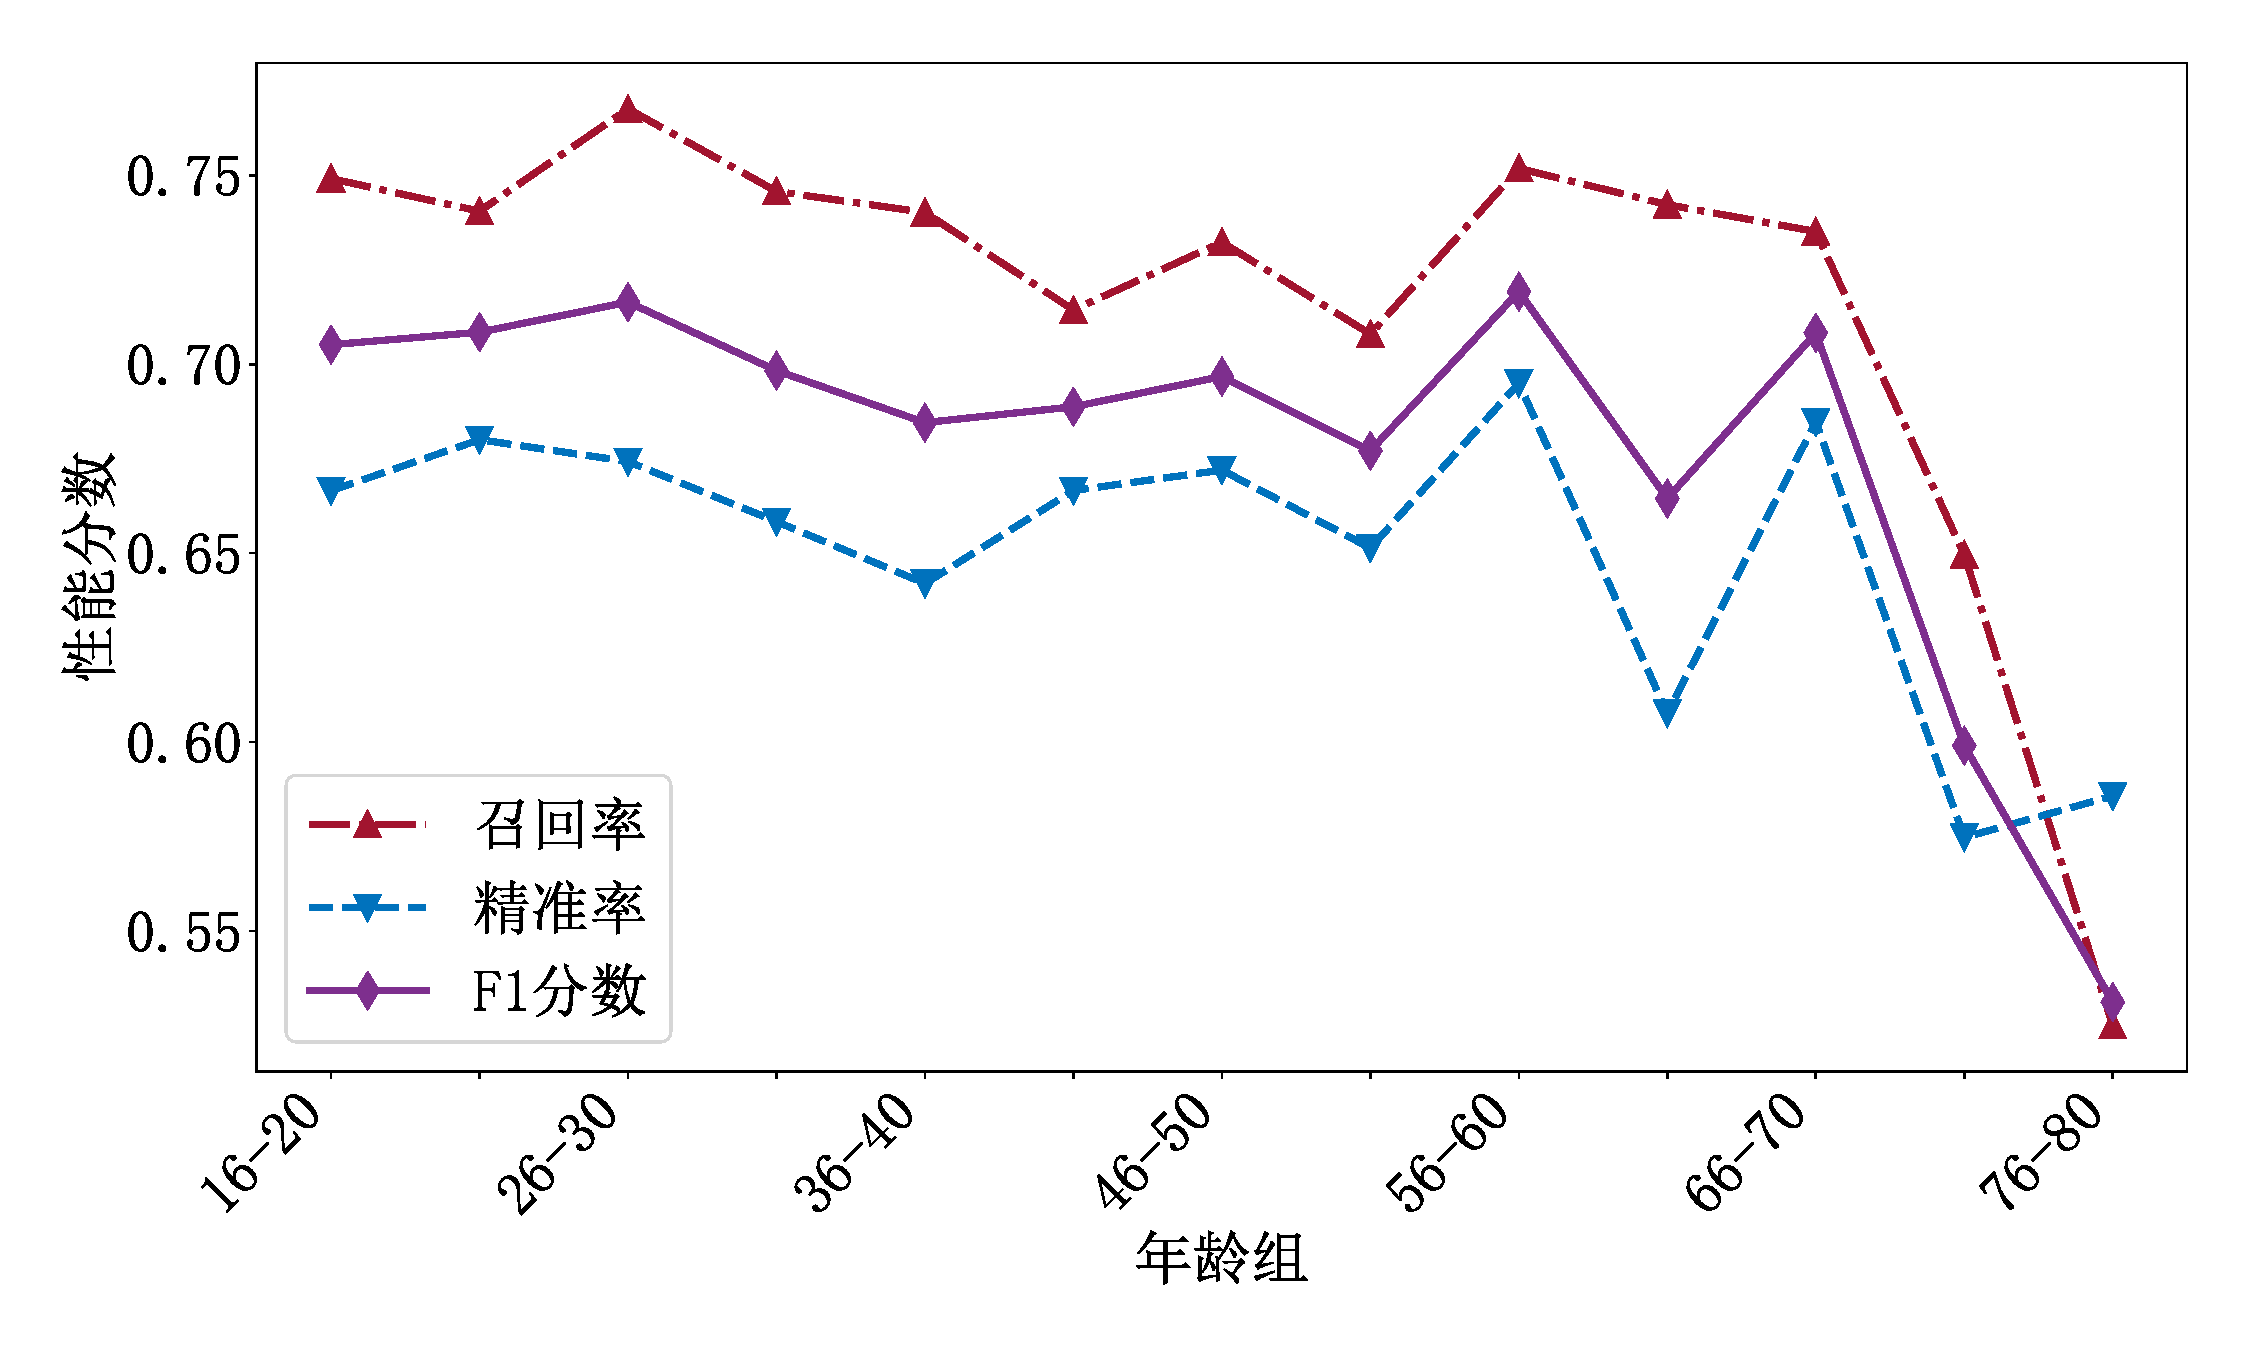
\includegraphics[width=1\textwidth]{Ms-ICCP_Impact-Age.pdf}
	\caption{年龄参数的影响}
	\label{Fig:Impact-Age}
\end{figure}
为了研究用户年龄的影响,我们将IC用户分为13个年龄组,年龄从16岁到80岁,每个年龄组的范围为5。图\ref{Fig:Impact-Age}显示了ICCP在不同年龄组中获得的召回率、精准率和F1分数的平均指标得分。虽然16岁至60岁用户的分数略有变化,但几乎所有的分数都在70\%以上,这意味着ICCP可以在所有用户上稳健运行,而不受用户年龄影响流量消耗。另外,对于16岁至35岁的用户,他们可以获得最高的精度分数,这是因为年轻用户在互联网服务中更活跃,他们在离开系统前的异常行为更容易被识别出来。另一方面,对于61岁至80岁的用户,我们可以看到指标得分有严重的抖动,这是因为老年用户在互联网服务中不太活跃,很难捕捉他们的网络使用行为。

\subsubsection{APP参数的影响}
\begin{figure}[hbt]
	\centering
	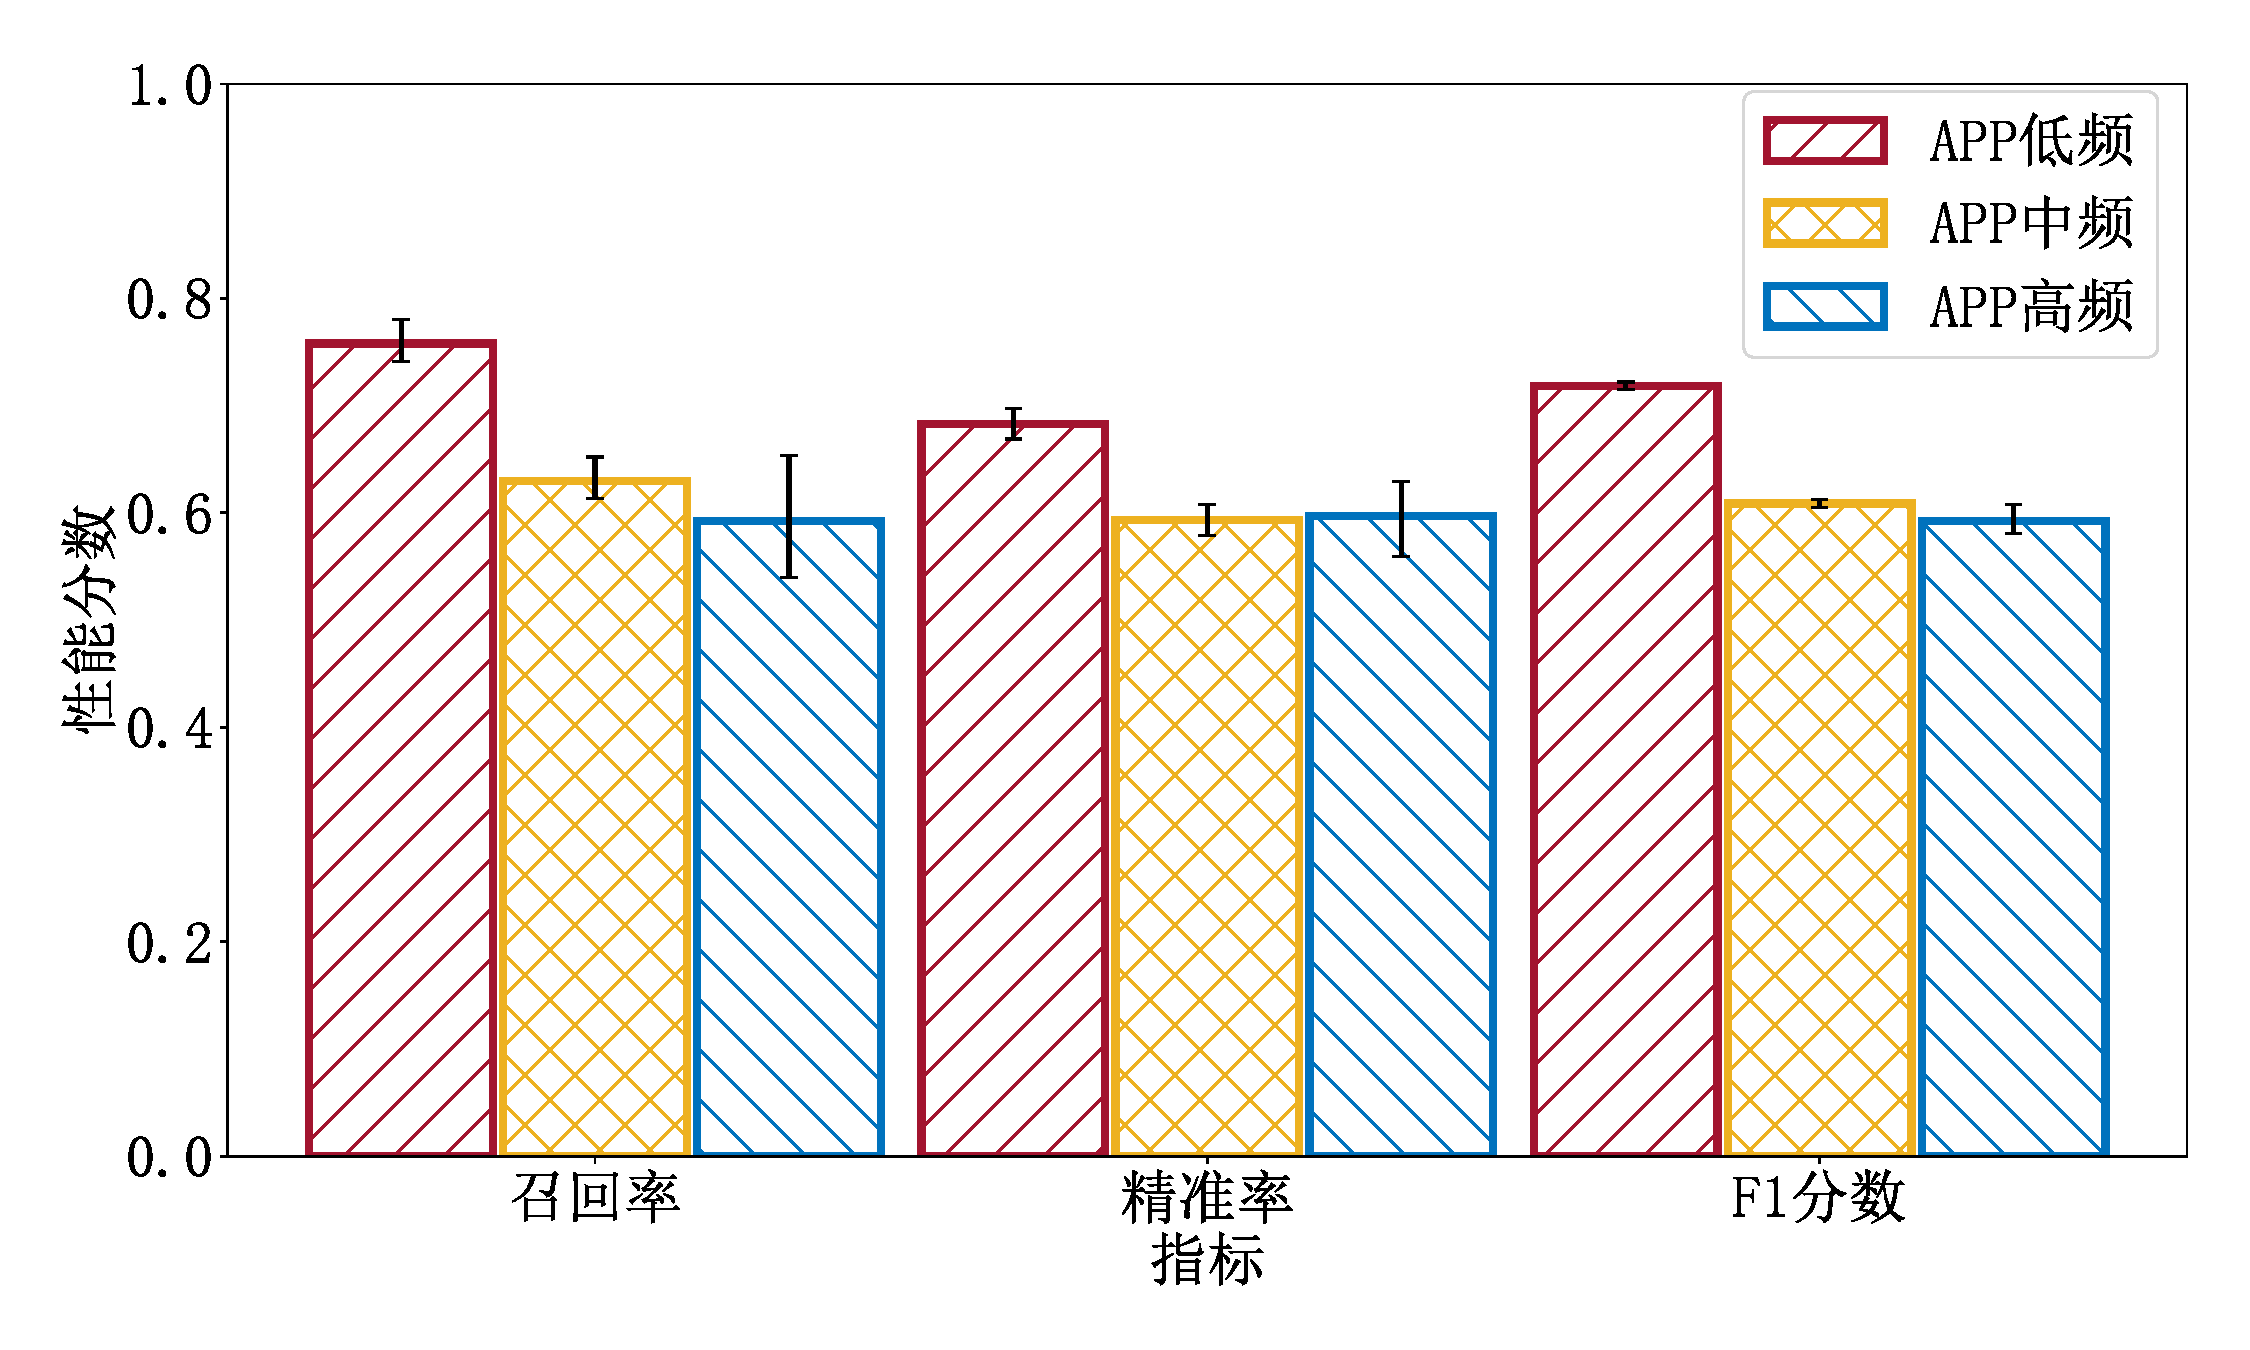
\includegraphics[width=1\textwidth]{Ms-ICCP_Impact-APP.pdf}
	\caption{APP参数的影响}
	\label{Fig:Impact-APP}
\end{figure}
我们通过对用户应用程序使用频率的排序,将用户样本分为三个级别,即:高、中、低。图\ref{Fig:Impact-APP}显示了采用k = 5的k折交叉验证方法对三组APP使用水平不同的互联网卡用户的平均度量得分和误差条。我们可以看到,ICCP在APP使用频率中等和较高的用户中都能很好地工作,这两个用户的指标得分非常相似。但是,我们可以观察到,APP使用频率较低用户的指标得分比其他App使用级别的用户要大,这与我们之前的分析是一致的,低App使用频率的特征可以有效区分出离网用户。例如,对于召回率、精确度和F1分数的指标,APP使用频率较低用户组可以分别获得0.76、0.68和0.72的平均分,APP使用频率中等用户组可以分别获得0.63、0.59和0.61的平均分,而APP使用频率较高用户组用户可以分别获得0.59、0.58和0.59的平均分。

\subsubsection{套餐参数的影响}
\begin{figure}[hbt]
	\centering
	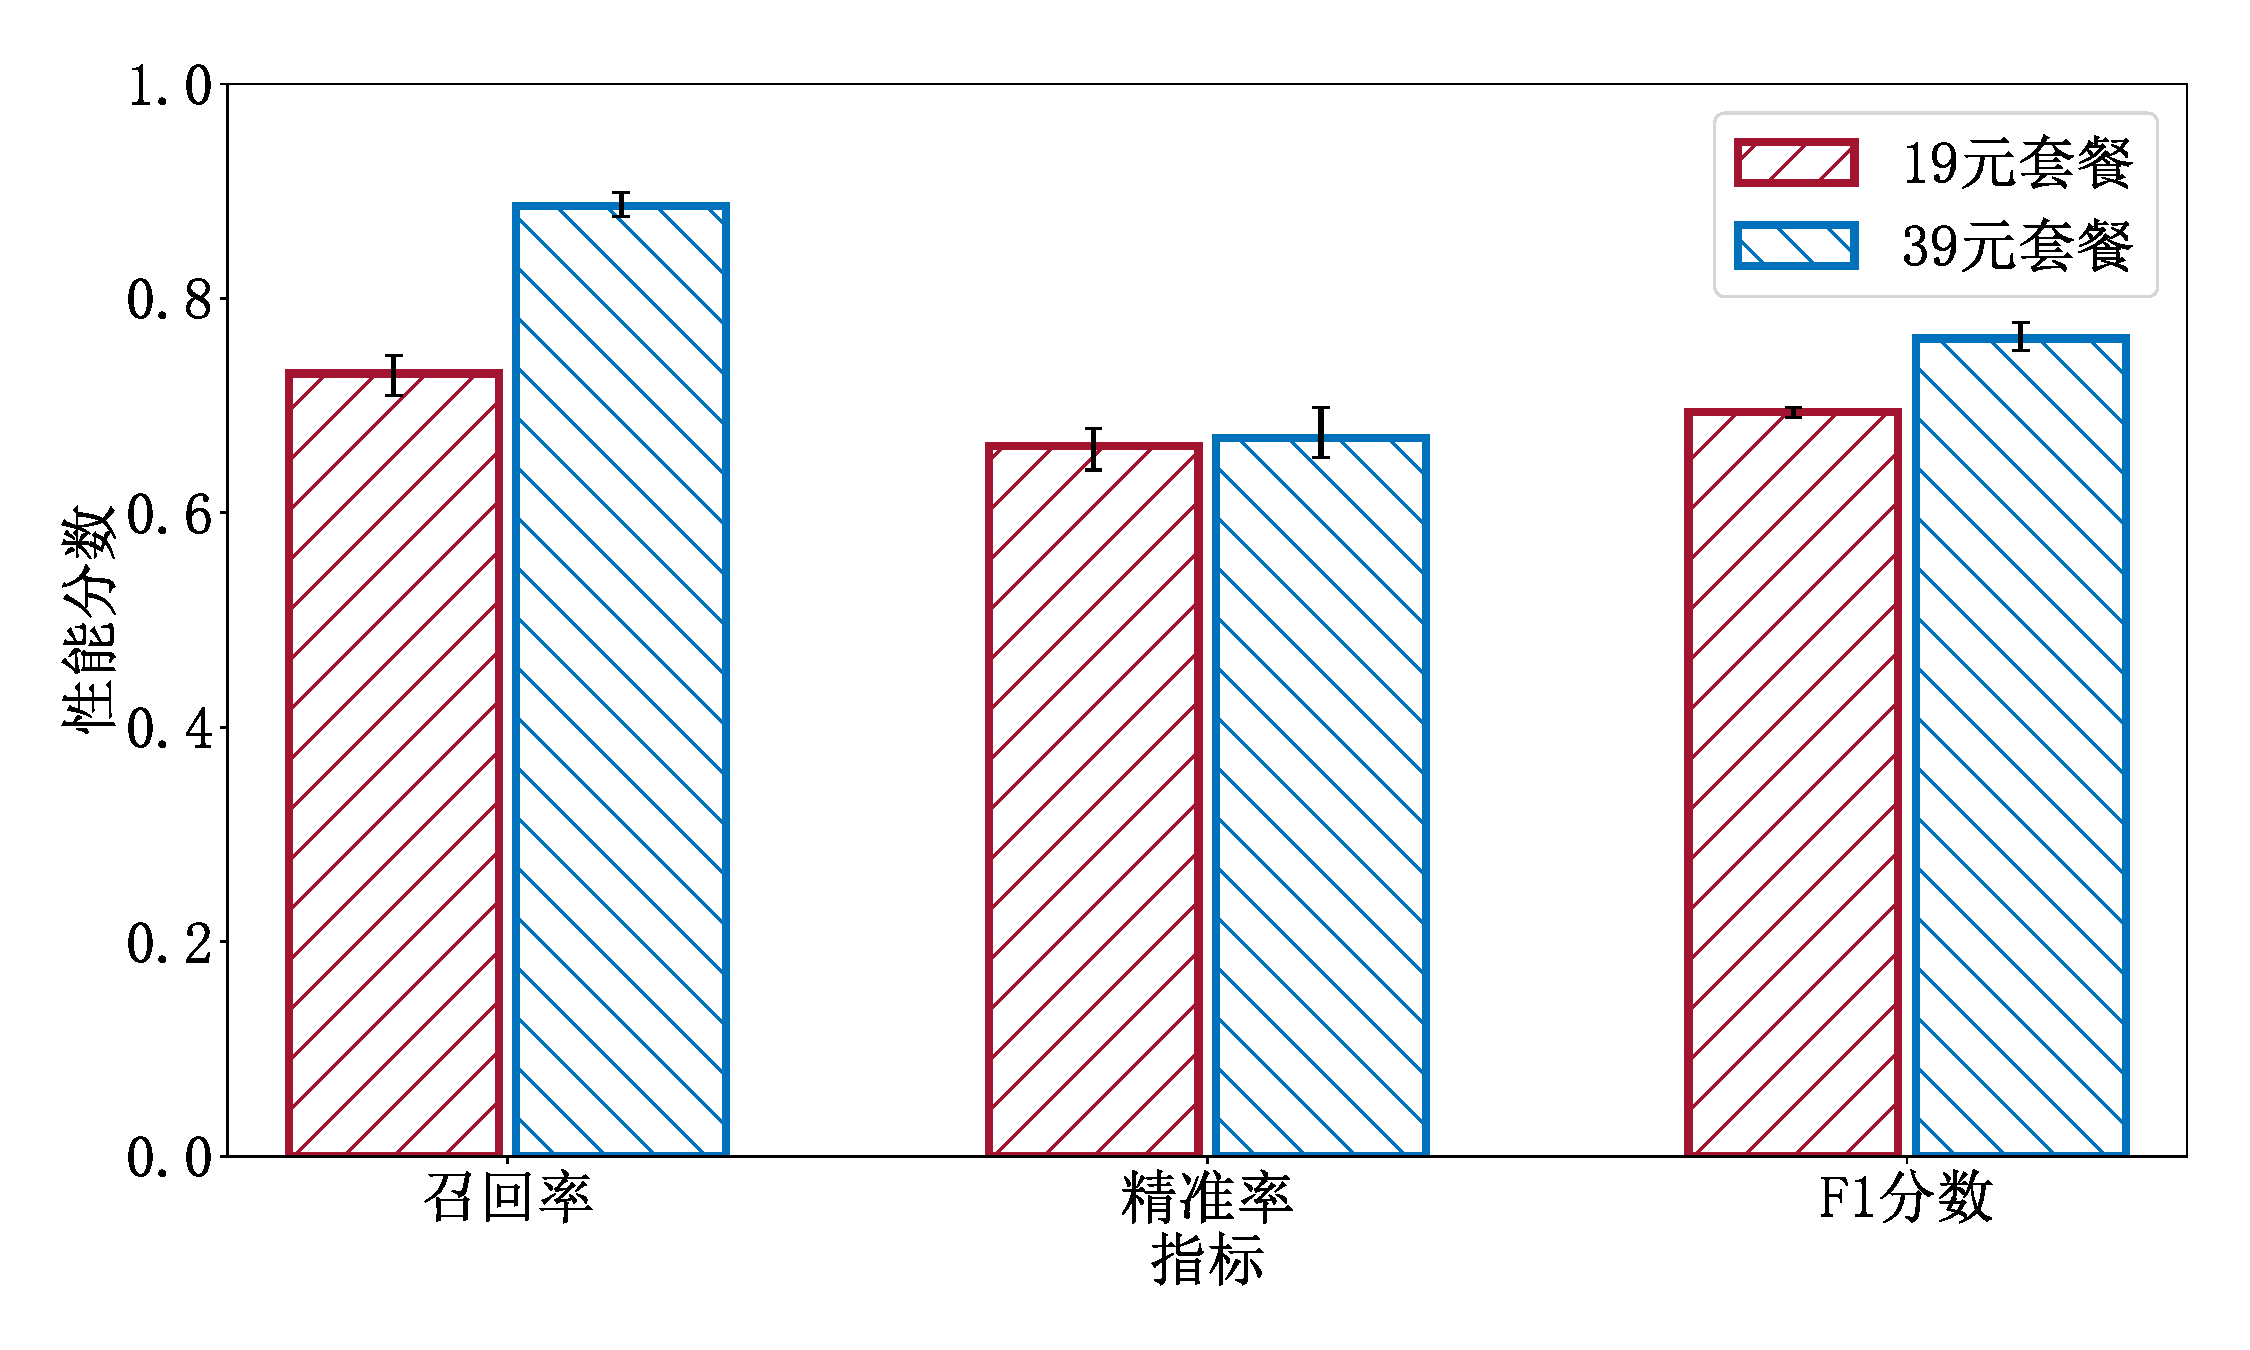
\includegraphics[width=1\textwidth]{Ms-ICCP_Impact-Combo.pdf}
	\caption{套餐参数的影响}
	\label{Fig:Impact-Combo}
\end{figure}
为了检验用户套餐选择的影响,我们采用k折交叉验证方法,用误差条图绘制前2个受欢迎套餐(例如,19元和39元)的平均度量分数,如图\ref{Fig:Impact-Combo}所示。我们可以观察到,ICCP对于这两种套餐的用户都可以稳健地工作,其中他们的精准率度量得分非常相似,并且与系统的总体性能相当。此外,我们可以看到39元套餐的指标得分(例如,召回率和F1分数)比19元套餐的用户略大,这是因为根据我们之前的分析,19元套餐比39元套餐有更多的离网用户,从而带来了更多的预测挑战。


\subsection{消融实验}
\begin{table}[htb]
	\centering
	\caption{消融实验}
	\label{Table:Ablation}
	\begin{tabular}{llllll}
		\toprule
		& AUC  & PR-AUC  & F1分数  & 召回率  & 精准率 \\
		\midrule 
		\midrule
		所有特征 	& 0.9754 & 0.7749 & 0.7022 & 0.7464 & 0.6630	\\
		-目标编码 	& 0.8656 & 0.4646 & 0.4548	& 0.4783 & 0.4335 	\\
		-账户余额 	& 0.9441 & 0.6420 & 0.5750	& 0.5795 & 0.5706	\\
		-CDR序列 	& 0.9727 & 0.7380 & 0.6781 & 0.7378 & 0.6274	\\
		-异常天数 	& 0.9752 & 0.7742 & 0.7014 & 0.7513 & 0.6577	\\
		-开卡月份 	 & 0.9745 & 0.7699 & 0.6970 & 0.7392 & 0.6593	\\
		-流量序列 	& 0.9735 & 0.7624 & 0.6912		& 0.7336 & 0.6535	\\
		-年龄 	& 0.9735 & 0.7624 & 0.6912	& 0.7336 & 0.6535	\\
		-活跃熵 	& 0.9439 & 0.6411 & 0.5716 & 0.6355 & 0.5195	\\
		-APP使用频次 & 0.9712 & 0.7321 & 0.6754	& 0.7668 & 0.6035	\\
		\midrule 
		\bottomrule	
	\end{tabular}
\end{table}

在本小节中,我们将进行消融实验来验证提取特征的有效性。消融实验结果如表\ref{Table:Ablation}所示。我们可以观察到,对于我们提取的主要特征,它们可以显著地影响预测性能,特别是目标编码和帐户余额这两个特征。特别是,当去除目标编码、账户余额和活跃熵特征时,精度从0.6630下降到0.4335、0.5706和0.5195,性能分别下降34.6\%、13.9\%和21.6\%。同样地,对于F1分数和召回率,分数可以分别从0.7022降低到0.4548、0.5750和0.5716,从0.7464降低到0.4783、0.5795和0.6355。

%\subsection{本章小结}
\newpage

\section{用户离网偏好感知的干预匹配算法设计}
%\section{基于汤普森采样的预离网用户干预算法设计}
%\section{预离网用户偏好生成算法设计}
\subsection{模块描述}
\begin{figure}[hbt]
	\centering
	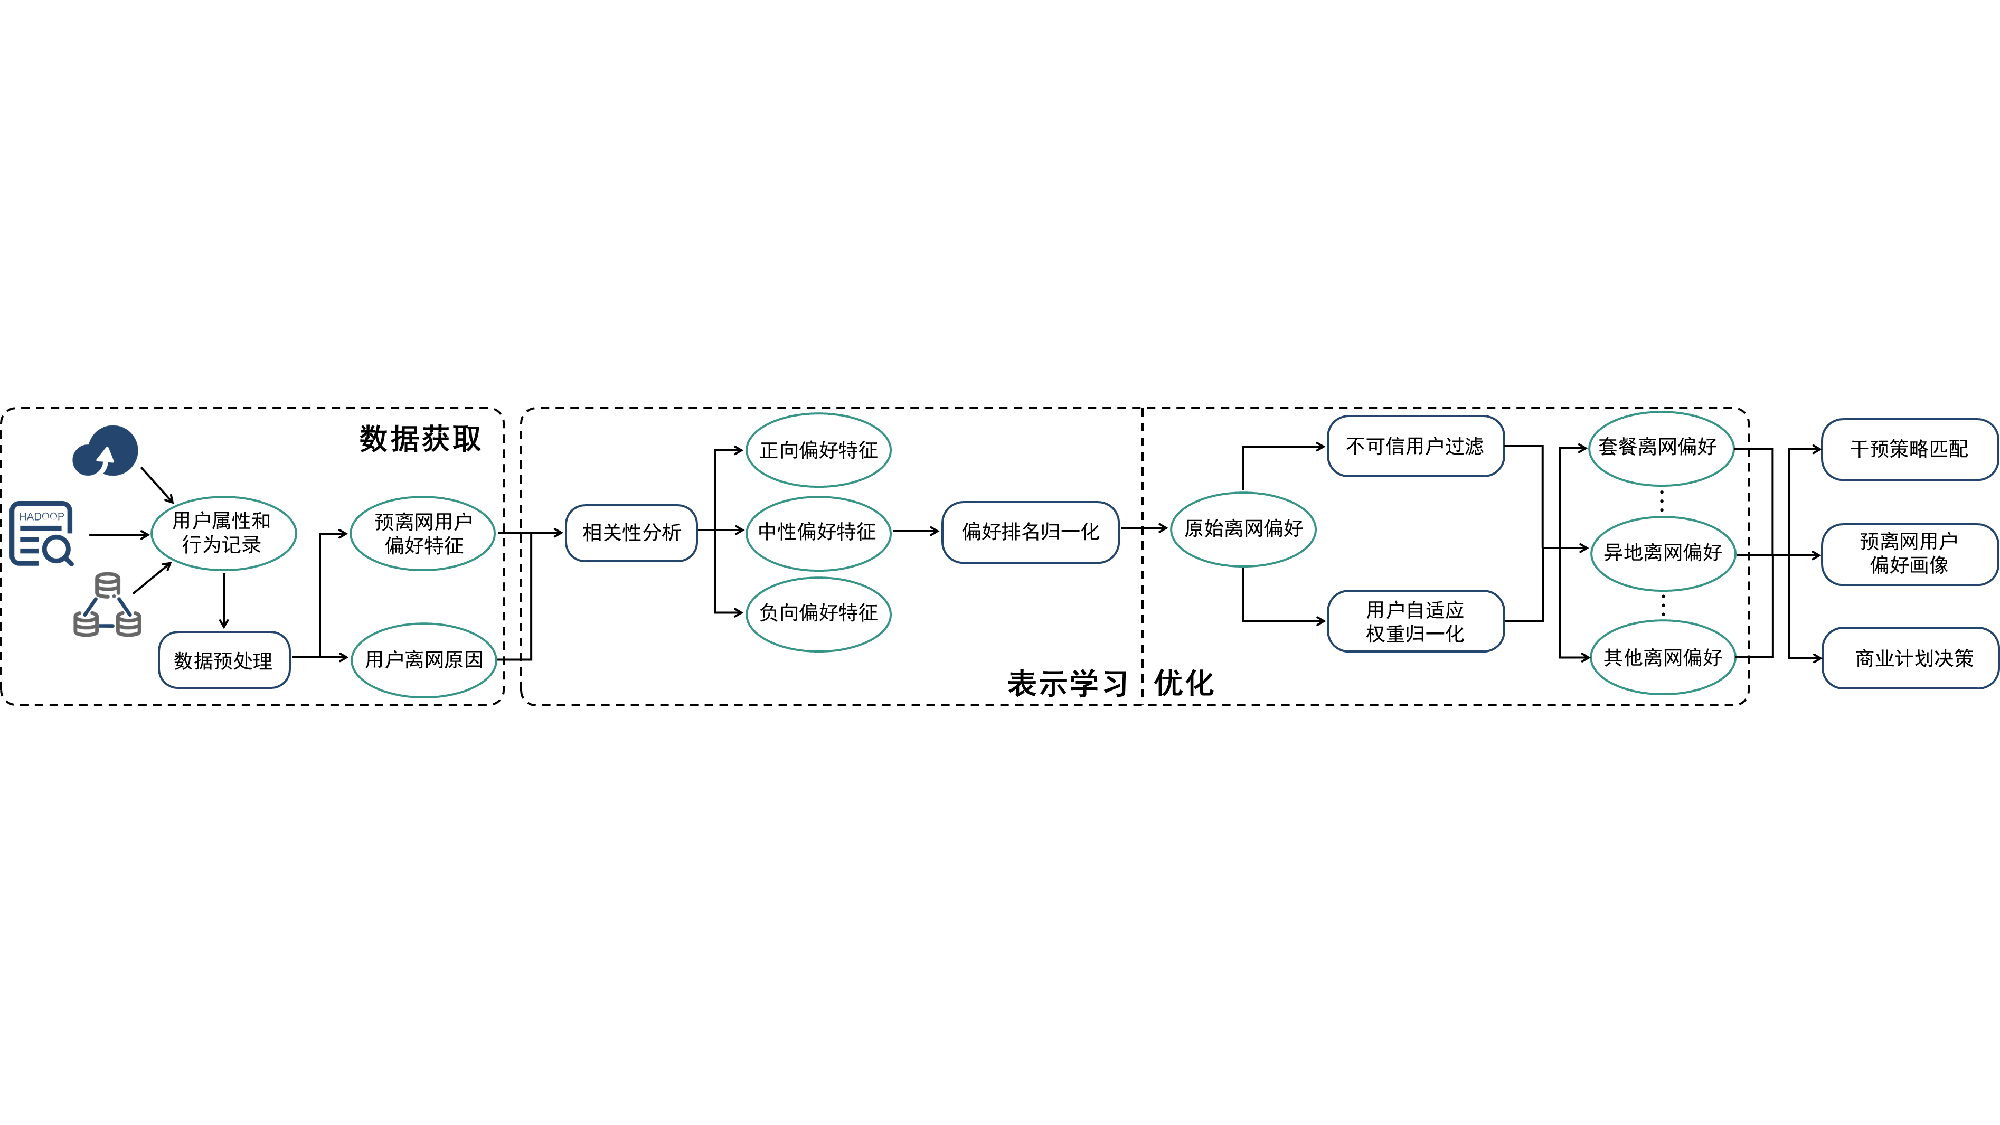
\includegraphics[width=1\textwidth]{Ms-ICSM_Preference-Module_v1_1.pdf}
	\caption{预离网用户偏好生成模块图}
	\label{Fig:Preference-Module}
\end{figure}

离网偏好模块的目标是找到一个准确的、可解释的表示法来表示离网预测模块给出的预离网用户的离网偏好。因此,我们首先限制了可用数据所能反映的离网原因的范围。在此基础上,运用耦合分析方法检验了各离网原因的独立性。接下来,我们通过提出的偏好排序归一化技术提取用户离网偏好。最后,对不可靠用户进行筛选,并实现用户自适应的权重归一化技术,来表征预离网用户的离网偏好。


\subsection{离网原因与偏好的相关性分析}
\begin{figure}[hbt]
	\centering
	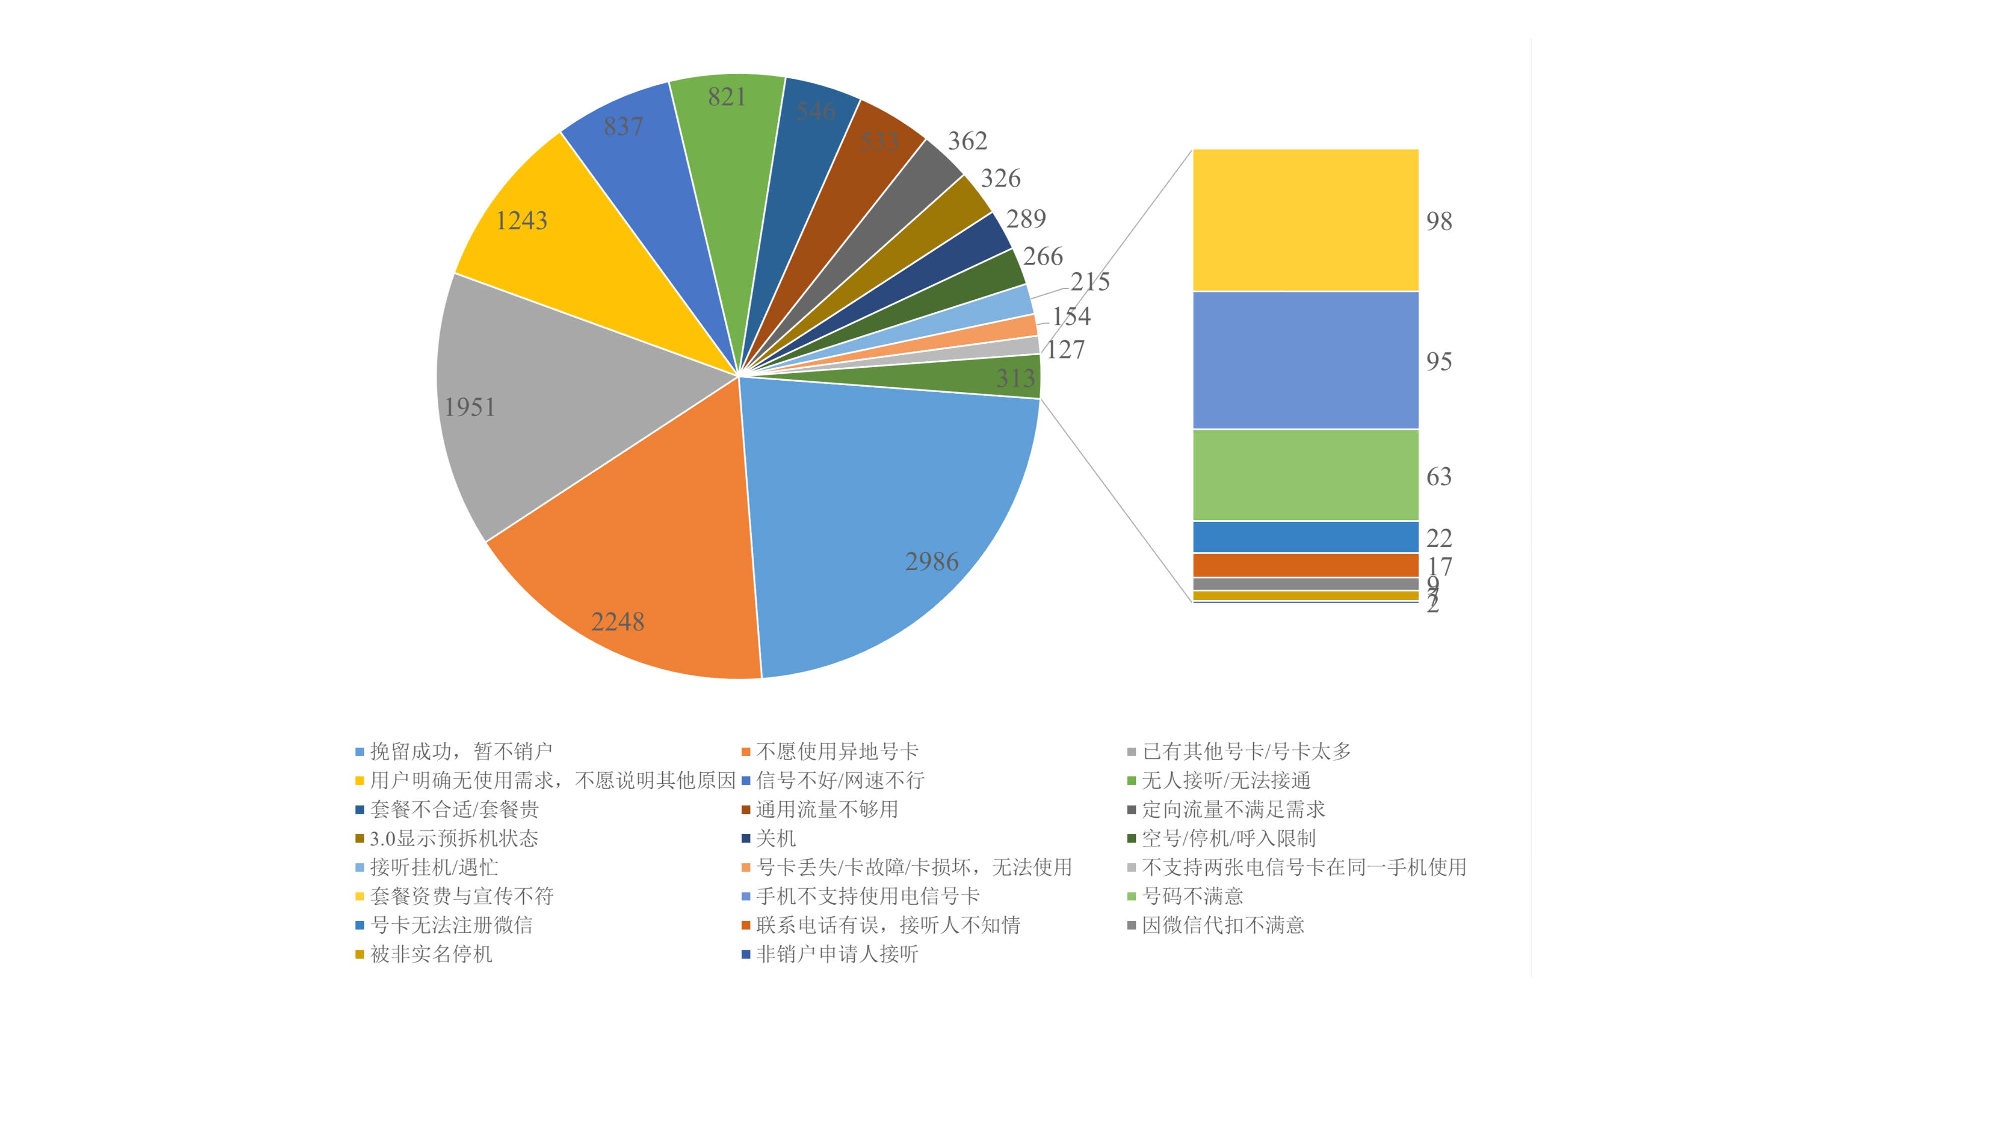
\includegraphics[width=1\textwidth]{Ms-ICSM_All-Churn-Reason_v1_1.pdf}
	\caption{互联网卡用户所有离网原因示意图}
	\label{Fig:All-Churn-Reason}
\end{figure}
如图\ref{Fig:All-Churn-Reason}所示为互联网卡用户离网原因分布,从中可以看出,离网原因有几十种,且各不相同。因此,我们选取用户数量排名前10位的离网原因,并绘制出相应的分布。

\begin{figure}[hbt]
	\centering
%	\includegraphics[width=1\textwidth]{Ms-ICSM_Top10-Churn-Reason_v2.pdf}
	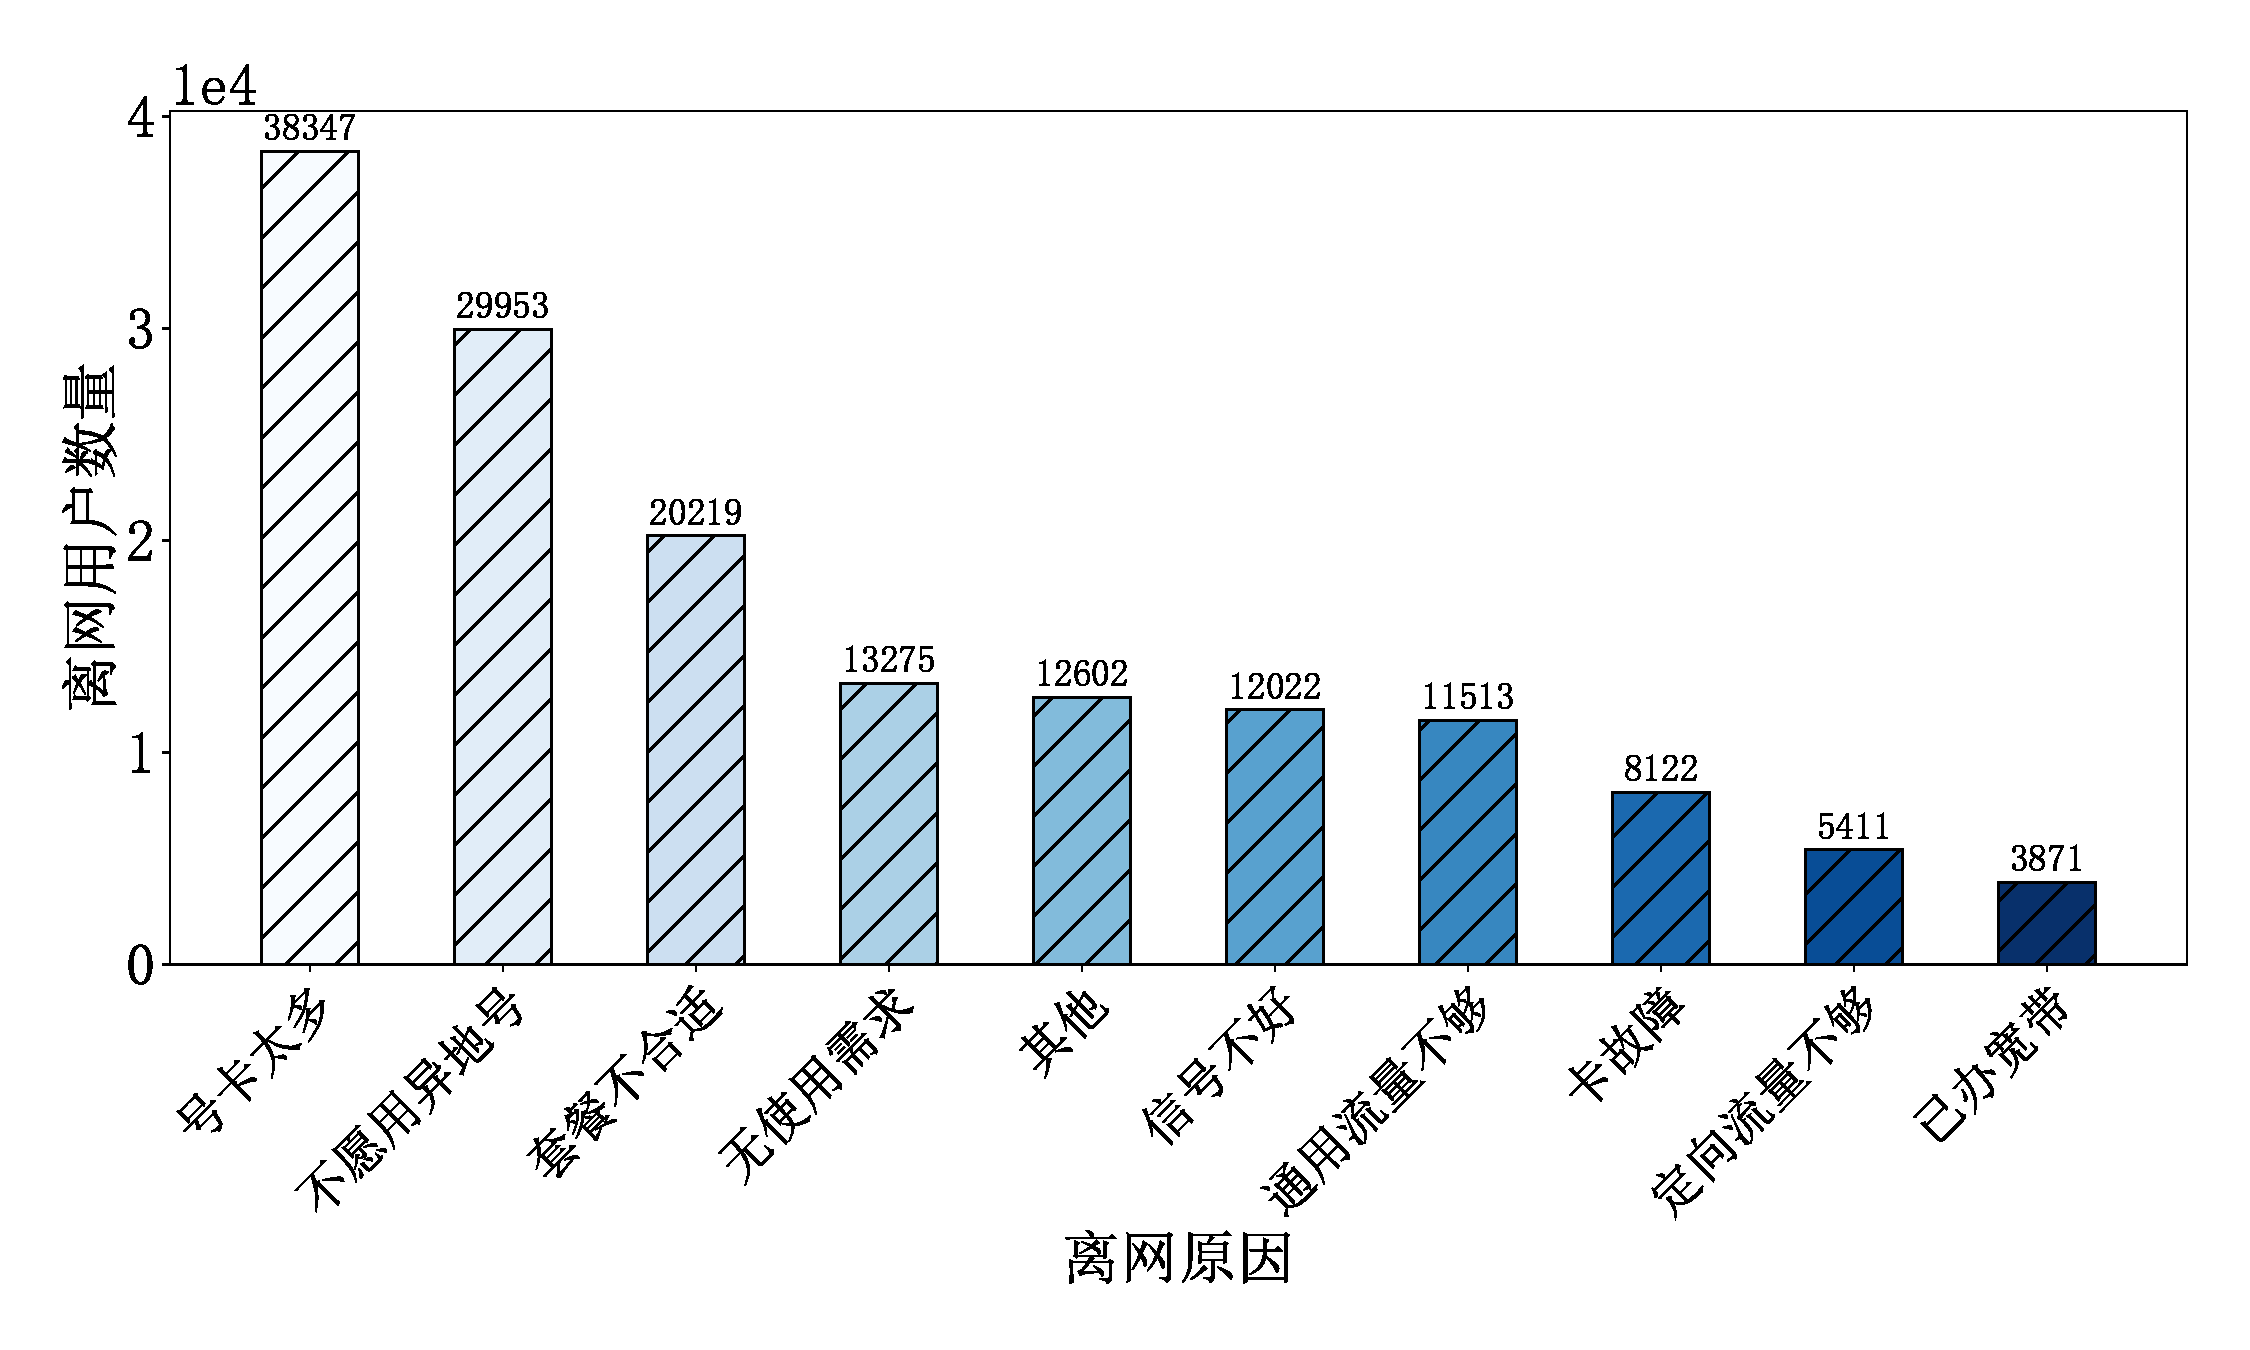
\includegraphics[width=1\textwidth]{Ms-Data_Top10-Churn-Reason_v2.pdf}
	\caption{互联网卡用户可建模的离网原因示意图}
	\label{Fig:ICSM-Top10-Churn-Reason}
\end{figure}
如图\ref{Fig:ICSM-Top10-Churn-Reason}所示,离网原因服从长尾分布,前10名离网原因的人数占总离网原因人数的90\%。因此,我们选择前10个离网原因来代表互联网卡用户的离网偏好是合理的。然而,由于现有数据表达能力有限,我们在10大离网原因中取消了5个,分别是号卡太多,无使用需求,其他,卡故障和已办宽带。


我们想知道,单一的离网原因是否可以完全代表预离网用户的离网偏好。因此,本文选取20万个离网用户来计算每两个离网原因之间的重叠程度。\\
我们用杰卡德相似系数来计算重叠度,计算公式\eqref{Eq:Jaccard-Similarit-Coefficient}如下式所示。
\begin{equation}
	\begin{aligned}
		J(R_{A}, R_{B}) = \frac{| R_{A} \cap R_{B} |}{| R_{A} \cup R_{B} |}
	\end{aligned}
	\label{Eq:Jaccard-Similarit-Coefficient}
\end{equation}
其中$R_{A},  R_{B}$分别表示因为离网原因A和B的离网用户id集合。


\begin{tabular}{cccccc}
	\toprule
	\ & 套餐不合适 & 信号不好 & 异地号卡 & 通用流量不够 & 定向流量不够 \\
	\midrule
	套餐不合适 & 1 & 0.04  & 0.63 & 0.71 & 0.06 \\
	信号不好 & - & 1 & 0 & 0 & 0 \\
	异地号卡 & - & - & 1 & 0.75 & 0.05 \\
	通用流量不够 & - & - & - & 1 & 0 \\
	定向流量不够 & - & -  & - & - & 1 \\
	\bottomrule
	%		\captionsetup{type=table}
	%		\caption{Coupled-Analysis Based on Jaccard Similarity Coefficient}
	\label{Table:Coupled-Analysis}
\end{tabular}

从表\ref{Table:Coupled-Analysis}中,我们可以得出这样的结论:由于套餐昂贵、异地号卡、通用流量不足等原因高度重叠,从而一起导致了用户的离网。这个现象暗示我们,部分离网用户的离网原因分布与个人偏好相关,可能有多个离网原因导致用户离网。此外,因网速低或定向流量不足而离网的离网用户相对独立,而高使用频次和高消费的离网用户大多为具有显著维系价值的外地用户。\\
综上所述,本文需要一个不同权重的离网原因数据结构来捕捉潜在离网用户的离网偏好。严格来说,我们定义了一个离网原因向量$\overrightarrow{C p} = [r_{1}, ..., r_{n}]$,本文把这称之为叫做离网偏好向量,用来表示潜在离网用户的离网偏好。然后我们定义 $r_{i} \in \overrightarrow{C p}$ 表示潜在离网用户的第$i$个离网原因的权重,n表示离网原因的数量。因此,我们得到约束如下: $r^{1}_{c} + r^{2}_{c} + ... +r^{n}_{c} = 1$。具体来说,在我们的场景中,离网原因包括套餐昂贵、网速低、定向流量不足、非本地互联网卡和通用流量不足,即$n = 5$。


\subsection{离网偏好排名归一化}
\textbf{相关特征选择}\\

\begin{tabular}{cccccc}
	\toprule
	\ 离网原因 & 偏好特征1 & 相关性1 & 偏好特征2 & 相关性2 \\
	\midrule
	套餐不合适 & 出账金额 & 正向 & 账户余额 & 负向  \\
	信号不好 & 最大网速  & 负向 & 平均网速  & 负向 \\
	异地号卡 & 异地流量记录条数 & 正向 & 异地流量消耗值 & 正向 \\
	通用流量不够 & 通用流量记录条数 & 正向 & 通用流量消耗值 & 正向 \\
	定向流量不够 & 定向流量记录条数 & 正向 & 定向流量消耗值 & 正向 \\
	\bottomrule
	\label{Table:Correlation-Feature}
\end{tabular}
\\

我们首先人工选择与相应离网原因高度相关的偏好特征。例如,如表\ref{Table:Correlation-Feature}所示,我们为昂贵的套餐这个离网原因选择了出账金额和账户余额这两个偏好特征。

\textbf{等频分箱}\\

为了表示离网预测模块给出的预离网用户的离网偏好,我们要计算出某一特定预离网用户在所有潜在离网用户中所处的水平。具体来说,如果某个预离网用户$c$在某个特定离网原因$crf$所属的偏好特征上排名超过了绝大多数用户,那么我们假设该预离网用户$c$很有可能因为离网原因$crf$而离网。此外,由于每个偏好特征的分布和性质不同,本文需要一种方法来推导出能按比例地反映离网原因的权重。基于以上假设,我们采用等频分箱技术对表\ref{Table:Correlation-Feature}中的上述特征分别进行离散化处理。接着,本文能把每个偏好特征从值域$[min\_val, max\_val]$映射到值域$[1, n_{c}]$,其中$min\_val$, $max\_val$和$n_{c}$ 分别表示偏好特征的最小值,最大值和分箱数量。 在我们的设置当中, $n_{c} = 100$.

\textbf{双重排名归一化}\\

对于和对应离网原因是正相关关系的特征向量 $\vec{x}$来说, 特征$x$的排名向量 $\overrightarrow{R_x}$等于
\begin{equation}
	\begin{aligned}
		\overrightarrow{R_x} = \frac{\vec{x}-min\_val}{max\_val-min\_val}*(n_{c} - 1) + 1.
	\end{aligned}
	\label{Eq:Postive-Binning}
\end{equation}	

对于和对应离网原因是负相关关系的特征向量 $\vec{x}$来说, 特征$x$的排名向量 $\overrightarrow{R_y}$等于
\begin{equation}
	\begin{aligned}
		\overrightarrow{R_y} = \frac{\vec{y}-min\_val}{max\_val-min\_val}*(n_{c} - 1) + 1.
	\end{aligned}
	\label{Eq:Negative-Binning}
\end{equation}	

\subsection{离网偏好生成}
在推导出所有偏好特征的排名向量集合之后,我们可以计算出预离网用户的原始离网偏好向量
\begin{equation}
	\begin{aligned}
		%			\overrightarrow{C_{pr}} = \sum_{i=1}^{n}\sum_{j=1}^{2} 0.5 \times R_{ij}
		\overrightarrow{C_{pr}} =[pr_{1}, ..., pr_{n}] = concat(\sum_{j=1}^{2} 0.5 \times R_{ij}, for ~ i=1, ..., n).
	\end{aligned}
	\label{Eq:Jaccard-Similarit-Coefficient}
\end{equation}	
例如,预离网者$c$的原始离网偏好向量$\overrightarrow{C_{pr}}$可能等于[0.9,0.7,0.01,0.02,0.4],这意味着昂贵的套餐成本、低网速、定向流量不足、非本地互联网卡和通用流量不同的权重分别为0.9,0.7,0.01,0.02,0.4。

\subsubsection{不可信用户过滤机制}
首先,虽然离网预测模型已经过滤掉了大部分正常用户,但仍有少数正常用户被遗漏。其次,干预的预算有限,只能覆盖部分离网用户。第三,典型活跃离网用户的离网偏好特征的排序和要高得多。基于以上三个原因,我们在生成客户离网偏好模块之后设置了一个不可信用户过滤模块。具体来说,排名和小于预先定义的阈值$t$的预离网用户将被过滤,即离网偏好字段的平均排名小于$t/n$。由于这些预离网用户的离网偏好与其他预离网用户相比并不值得注意,这些预离网用户将被移除来保证有限预算的投资回报率(ROI)。

\subsubsection{自适应的权重归一化}
虽然预离网用户的离网偏好是个性化的,但对于每一个预离网用户,每个离网偏好的贡献率之和应该等于1。为了统一离网偏好向量元素的量级,我们采用改进的softmax函数,通过用户自适应的方式表示预离网用户的离网偏好向量$\overrightarrow{C_{p}}$,如下公式\ref{Eq:Self-Adaptive-Weight-Normalization}所示。
\begin{equation}
	\begin{aligned}
		\overrightarrow{C_{p}}  = \frac{e^{pr_{i}-max(\overrightarrow{C_{pr}})}}{\sum_{i=1}^{n} e^{pr_{i}-max(\overrightarrow{C_{pr}})}}
	\end{aligned}
	\label{Eq:Self-Adaptive-Weight-Normalization}
\end{equation}	
其中$max(\overrightarrow{C_{pr}})$ 表示原始离网偏好向量 $\overrightarrow{C_{pr}}$的最大值。 最后,我们可以获得预离网用户$c$的离网偏好向量 $\overrightarrow{C_{p}}_c$ 和预离网用户集$\mathcal{C}$的离网偏好矩阵$\overrightarrow{C_{p}}$。
\par

%\subsection{本章小结}
\newpage

%\section{基于汤普森采样的预离网用户干预算法设计}
\subsection{系统描述与问题建模}
\textbf{问题形式化}\par
为了建模匹配模块,我们首先需要把匹配问题形式化,以保证我们的框架能够泛化到其他不同应用场景并且用支持不同算法、模型等实现具体功能。以下是具体描述。\par
对于运营商等企业,他们会采取一些干预策略,如营销宣传、优惠政策等来维系预离网用户。为保持通用性,我们定义干预策略集$\vec{E} = [E_{0}, E_{1}, E_{2}, ..., E_{i},..., E_{M}]$,其中$0$表示不进行任何干预,$E_{i}$表示第i个的干预策略。在我们的情景中,干预策略可以分为以下四种:话费,流量,通话和APP。\par
为了使我们提出的框架能够感知预算,干预策略的成本被形式化为向量$\vec{E} = [E_{0}, E_{1}, E_{2}, ..., E_{i},..., E_{M}]$,其中$E_{i}$表示第i个干预策略的成本。其中,$E_{0} = 0$表示企业对预离网用户不做任何干预时,成本等于0。\par
对于在由离网预测模块给出的预离网用户集合$\mathcal{C}$中的任何一个预离网用户c,我们定义一个二元状态变量$y_{c}$来表示下个月该预离网用户c是否会真的离网,其中$y_{c}=1$表示下个月预离网用户c会离网,$y_{c}=0$则表示相反的意思。我们还定义了一个二元状态变量$z_{c}$来表示在执行干预后,预离网用户$c$是否被成功维系,其中$z_{c} = 1$表示预离网用户c被成功保留,$z_{c} = 0$则相反。$\vec{x_{c}}$ 被定义为企业实施到预离网用户$c$的干预策略。$\vec{x_{c}} = [x_{c0}, x_{c1}, ..., x_{cj}, ..., x_{cM}]$,其中 $x_{cj}=1$ 表示用户 $c$ 采用了第j个干预策略, $x_{cj}=0$表示相反. 需要特别指出的是,$x_{c0}=1$ 表示企业对预离网用户$c$不采取任何干预措施。\par
因此,匹配模块的优化目标可以形式化为
\begin{equation}
	\begin{aligned}
		& \max \sum_{c \in \mathcal{C}} y_{c}z_{c} \\
		& \mathrm{s.t.} \sum_{\forall c} \vec{x_{c}} \cdot \vec{E} \leq B , \\
		& LV_{c} \geq \vec{x_{c}} \cdot \vec{E}, \forall c			
	\end{aligned}
	\label{Eq:matching-target}
\end{equation}	
其中$B$表示为企业预算,  $LV_{c}$表示为预离网用户$c$的生命周期价值。\eqref{Eq:matching-target}代表的意义为在企业预先给定的预算$B$的前提下,基于我们预算感知的框架,我们的目标是最大化干预成功的离网用户数。 第一个约束意味着所有的干预策略投入成本和要小于等于预算$B$. 第二个约束旨在通过限制投入到预离网用户$c$的成本之和要小于等于其生命周期价值的贪婪方式来保证最后最终收益是非负的。\par
\textbf{设计思想}\par
	我们对于匹配模块的设计思想是把挽留策略匹配问题建模成一个多臂老虎机问题。
	原因如下:
\begin{enumerate}	
	\item 我们只给每个用户匹配一个挽留策略。
	\item 假设每个挽留策略对某个用户是否干预成功的指示变量 是服从某一概率分布的, 但是每个挽留策略不一定是独立的,所以不同的拉杆之间可能有耦合关系。 
	\item 目的是最大化挽留收益。这些都符合典型的多臂老虎机问题设置,一次操作对应一个用户, 一个拉杆对应一个挽留策略, 老虎机的累积奖励对应企业的最终挽留收益。
\end{enumerate}
	基于上述原因,我们设计了如下架构。首先我们生成一个奖励模型用以给匹配算法提供基于用户离网偏好的反馈从而弥补缺失直接用户偏好数据的问题。然后我们通过离线训练挽留策略匹配模型来使它学习不同离网偏好的预离网用户的挽留策略偏好。
%	最后, 我们开展了一个基于生成数据的在线学习。

\begin{figure}[hbt]
	\centering
	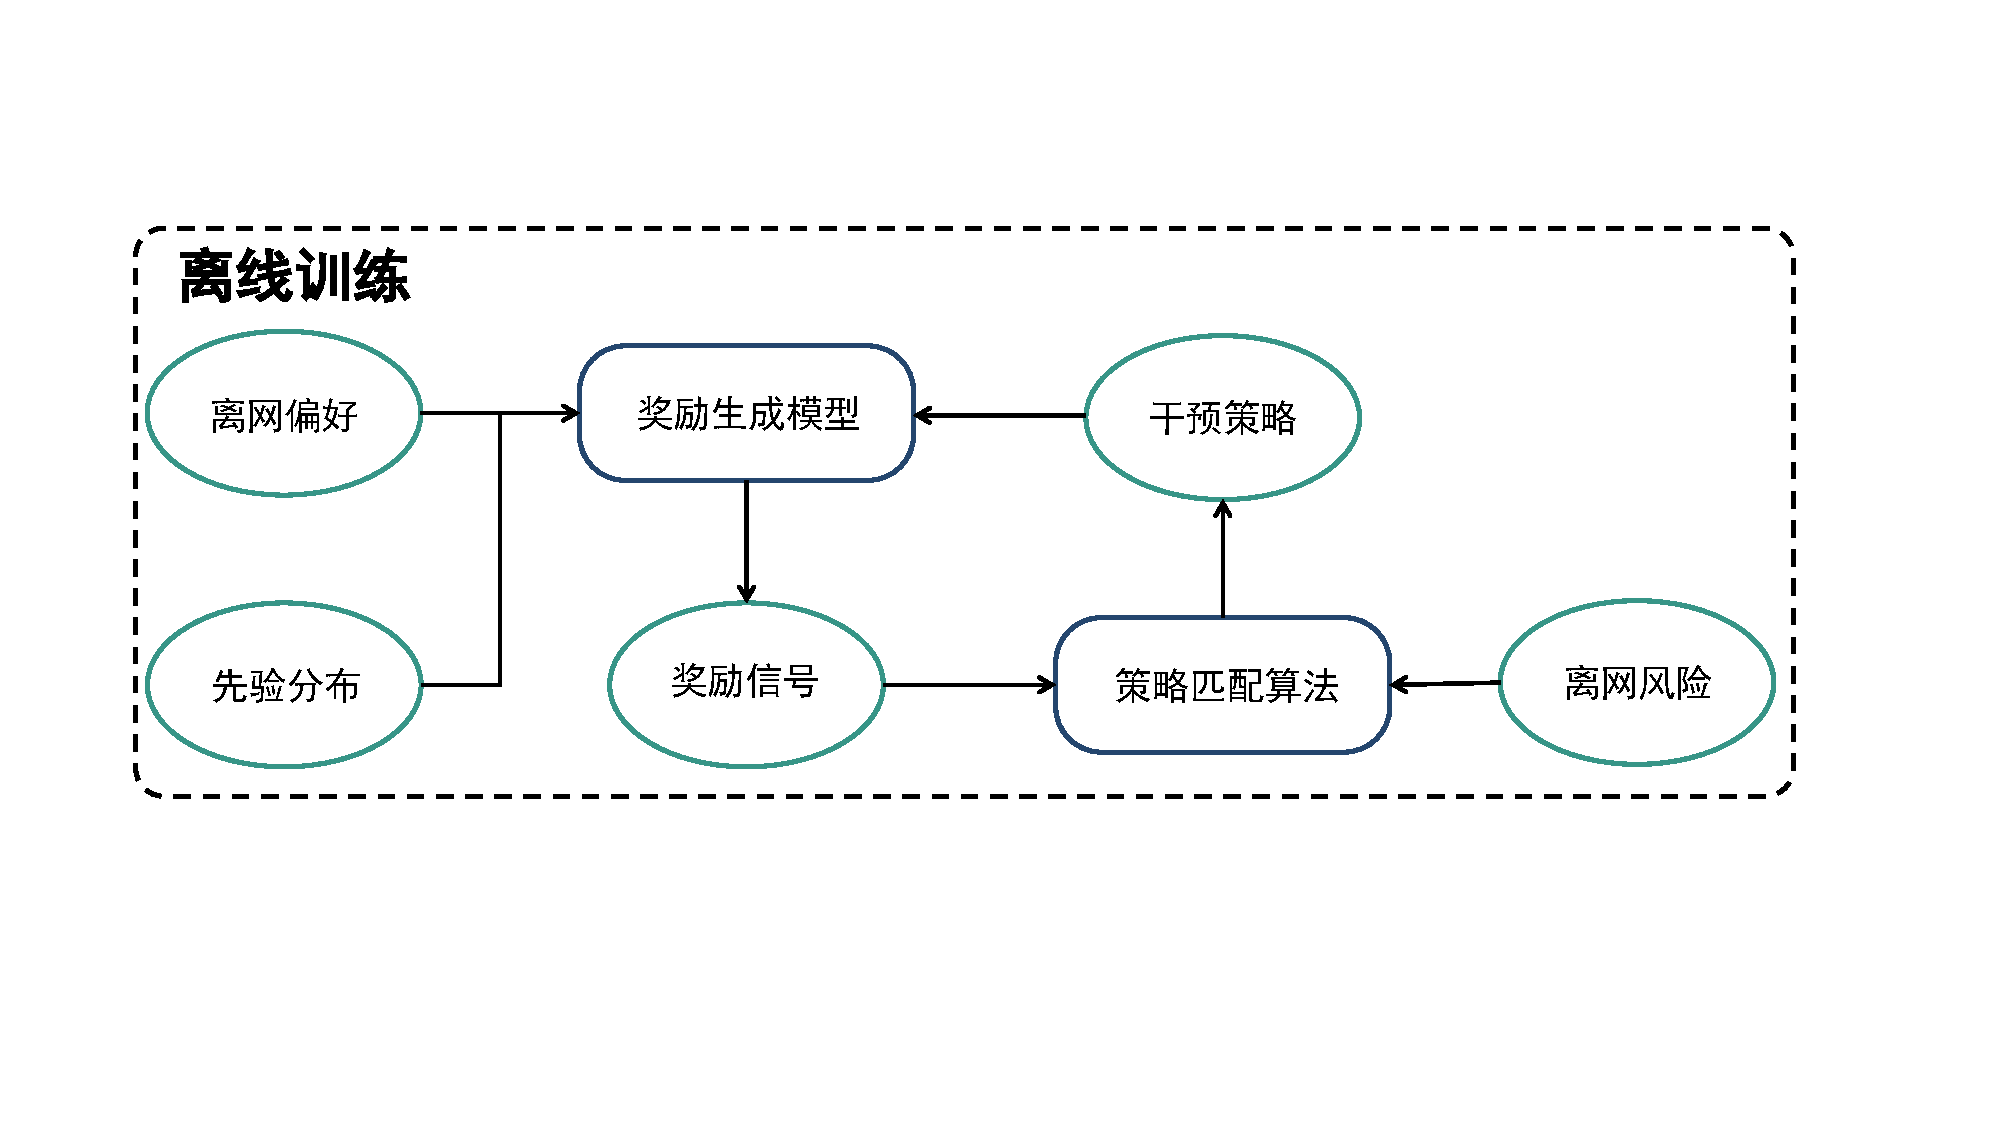
\includegraphics[width=1\textwidth]{Ms-ICSM_Matching-Module_v1_1.pdf}
	\caption{干预策略匹配模块图}
	\label{Fig:Matching-Module}
\end{figure}

\subsection{奖励生成模型设计}

\begin{figure}[hbt]
	\centering
	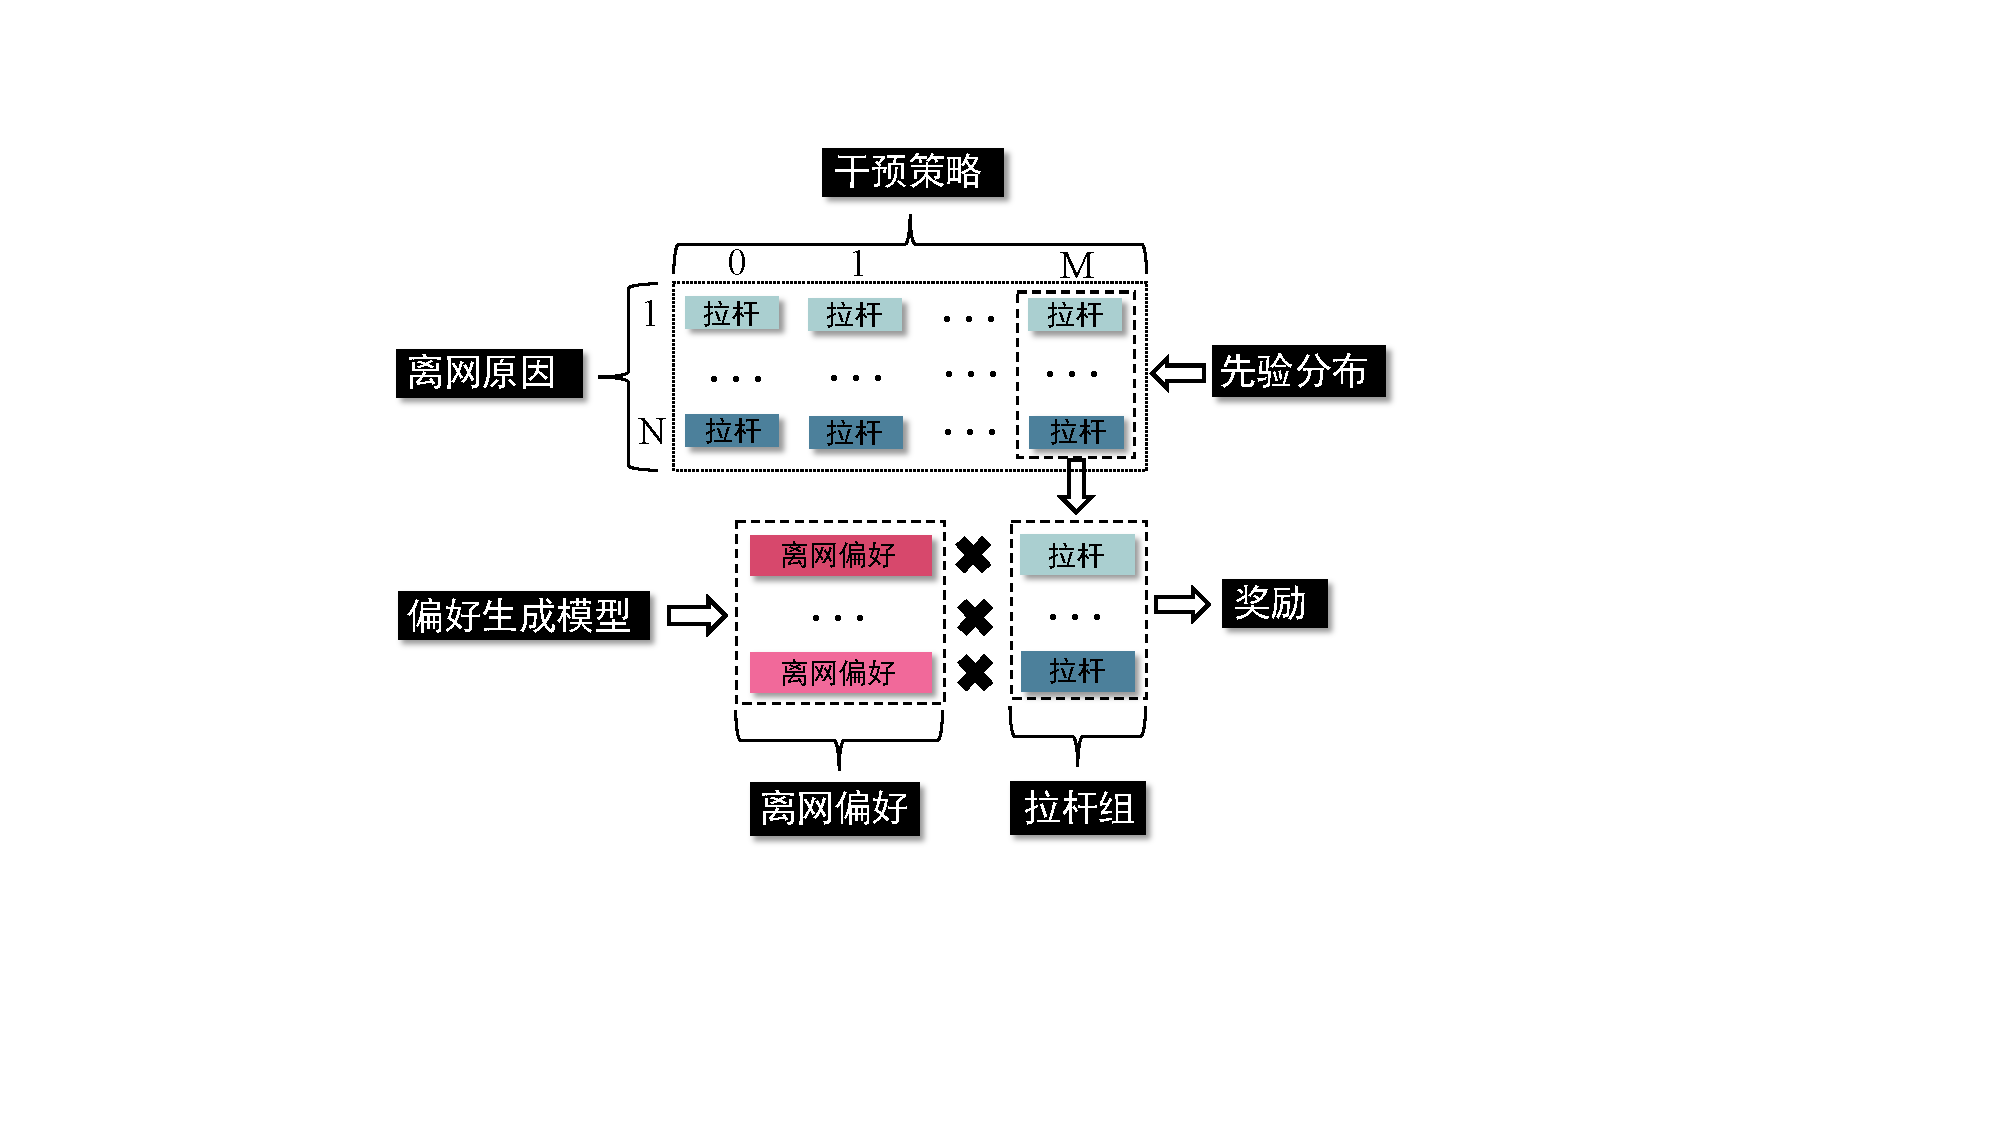
\includegraphics[width=1\textwidth]{Ms-ICSM_Reward-Model_v1_1.pdf}
	\caption{奖励模型内部示意图}
	\label{Fig:Reward-Model}
\end{figure}
基于以下三个原因,我们设计了奖励生成模型。
\begin{enumerate}	
	\item 我们的数据缺乏直接的干预记录,如客户id、匹配的干预策略、干预结果等。然而,我们获得了不同离网原因所匹配的干预策略成功概率的统计数据。
	\item 受基于人类反馈的强化学习(RLHF)的启发,我们设计的这个模块可以通过接受预离网用户的离网偏好来生成反映人类偏好的奖励。
	\item 由于干预记录数据的稀疏性,奖励生成模型可以生成合成数据用于训练后续算法,以降低相关数据的收集和清理成本。
\end{enumerate}
\par
为此,我们实现了一种接受预离网用户的离网偏好和相应的干预策略作为输入,并返回信号值作为奖励的多臂老虎机MAB。因此,奖励生成模型的拉杆数量需要满足约束
\begin{equation}
	\begin{aligned}
		\#. ~ arms = (M + 1) \times N
	\end{aligned}
	\label{Eq:bandit-constraint}
\end{equation}	
,其中$N$ 为离网原因数, $M$为干预策略数。具体而言,如图\ref{Fig:Reward-Model}所示,奖励生成模型有$N$行和$M+1$列的拉杆,其中 $arm_{ij}$表示对于因为离网原因i离网的用户匹配干预策略j的奖励期望。一列的拉杆被合称为一个拉杆组。\par
奖励生成模型中的拉杆可以被任意分布初始化,包括领域知识分布、均匀分布、高斯分布、二项分布、伽玛分布、泊松分布和指数分布等。由于我们统计了不同离网原因对应的干预策略成功概率。我们可以设定上述分布的期望等于平均成功概率。对于基于领域知识的分布,我们用不同离网原因对应的干预策略平均成功概率填充。\par
	
	接下里,本文会介绍产生被称为奖励的信号值的机制。首先,离网偏好模块将输出预离网用户$c$的离网偏好向量$\vec{Cp_{c}}$。
	其次,策略匹配算法将匹配预离网用户$c$以干预策略$s_{c}$。
	接着,奖励生成模型将干预策略$s_{c}$作为输入,然后选择相应的拉杆组。
	然后,奖励生成模型将离网偏好向量$\vec{Cp_{c}}$与拉杆组$\vec{Ag_{c}}$的点积计算为干预策略$s_{c}$的奖励期望,如公式\eqref{Eq:Reward-Expectation-Generation}所示。	 
\begin{equation}
	\begin{aligned}
		\mathbb{E}_{s_{c}} = \vec{Cp_{c}} \cdot \vec{Ag_{c}}
	\end{aligned}
	\label{Eq:Reward-Expectation-Generation}
\end{equation}
最后,奖励生成模型将根据0到1的均匀分布生成随机数$rn$。如果生成的随机数小于或等于点积,奖励生成模型将返回奖励$r_{c}=1$,否则为$r_{c}=0$。具体可见公式\eqref{Eq:reward-mechanism} 
\begin{equation}
	\begin{aligned}
		r_{c} = 
		\begin{cases}
			1, ~~if ~~ \mathbb{E}_{s_{c}} \leq rn \\
			0 ,~~otherwise
		\end{cases}
	\end{aligned}
	\label{Eq:reward-mechanism}
\end{equation}		
由公式\eqref{Eq:reward-mechanism} 可知,单个干预策略的维系成功概率服从伯努利分布。
假设有$M+1$个干预策略,那么我们如果尝试匹配无限次的话,我们将得到所有干预策略的平均奖励集合$\theta = (\theta_{0}, ..., \theta_{M})$。
接下来,如果策略匹配算法选择一个干预策略$s$,那么我们可以得到一个奖励$r \in \{0, 1\}$,这实际上是从伯努利分布中抽取的样本。换句话说,$\mathbb{P}[r=1|s \theta] = \theta_{s} $并且$\mathbb{P}[r=0|s, \theta] = 1-\theta_{s} $,这与观测到的事实是一致的。


\subsection{基于汤普森采样的用户-干预措施匹配算法设计}
\subsubsection{问题建模}
	在本文的场景中,多臂老虎机问题可以表示为五元组$\langle \mathcal{A}, \mathcal{E}, \mathcal{C}, \mathcal{A}^{'}, \mathcal{R}\rangle$ . \par
	\textbf{代理(Agent)($\mathcal{A}$).}  
	MAB问题的目标是最大化离网预测模块在预离网用户集$\mathcal{C}$中收集的累积奖励,如下所示。
	\begin{equation}
		\begin{aligned}
			& \max \sum_{c \in \mathcal{C}} y_{c} r_{c}, ~ s_{c} \sim \mathcal{R}(\cdot|s_{c}) \\
			& \mathrm{s.t.} ~ E_{s_{c}} \leq B ,\\
			& LV_{c} \geq E_{s_{c}}, \forall c			
		\end{aligned}
		\label{Eq:bandit-target}
	\end{equation}		
	公式\eqref{Eq:bandit-target}是公式\eqref{Eq:matching-target}的具体实现之一,其中$s_{c}$, $r_{c}$分别表示与预离网用户${c}$匹配的干预策略,匹配干预策略$s_{c}$所得的奖励。

\par
\textbf{环境(Environment)($\mathcal{E}$).} 
$\mathcal{E}$包含用户侧信息和项目侧信息。更具体地说,我们接受离网预测模块生成的预离网用户集合$\mathcal{C}$作为用户侧信息。此外,我们将干预策略集$\mathcal{S}$定义为物品侧信息,这其也是干预策略集$\mathcal{M}$的具体实现。
因此,干预策略空间等于集合$\{s_{0}, ..., s_{M}\}$,我们定义了$s_{m} \in \mathcal{S}$来表示任何在干预策略空间的中干预策略。相应的,干预策略集的代价集形式化为向量$\vec{E} = [E_{0}, E_{1}, E_{2}, ..., E_{i},..., E_{M}]$,其中$E_{i}$表示第i个干预策略的成本。需要特别指出的是,其中$E_{0} = 0$表示企业在预离网用户上不做任何干预时,成本等于0。 \par
\par

\textbf{上下文(Context)($\mathcal{C}$).} 
首先也是最重要的,我们引入预算$B$,以设置一个反映实际应用中资源有限的环境。此外,我们定义了离网偏好模块给出的离网偏好矩阵$Cp$和离网预测模块给出的离网风险向量$\vec{Cr}$作为上下文信息,使所提出的框架具有上下文感知能力,从而提高整体性能。

\par
\textbf{动作(Action)($\mathcal{A}^{'}$).}
由于匹配干预策略对应于拉动杠杆,我们定义多臂老虎机中有$M+1$个拉杆。正式来说,我们将可用拉杆集合定义为干预策略集$\mathcal{S}$。
\par
\textbf{奖励(Reward)($\mathcal{R}$).}
对于每一个干预策略$s$,我们定义了它的期望回报为
\begin{equation}
	\begin{aligned}
		Q(s) = \mathbb{E}_{s \sim \mathcal{R}(\cdot|s)} [r]
	\end{aligned}
	\label{Eq:Reward-Expectation}
\end{equation} 
。
因此,当离网用户具有确定的离网偏好时,至少存在一种干预策略的奖励期望大于或等于其他干预策略的奖励期望。
我们定义最佳奖励期望为
\begin{equation}
	\begin{aligned}
		Q^{*} = max_{s \in S}Q(s)
	\end{aligned}
	\label{Eq:Best-Reward-Expectation}
\end{equation}	
。
我们引入当前干预策略的懊悔,即当前干预策略的奖励期望与最佳干预策略的奖励期望之差,可被以下公式计算
\begin{equation}
	\begin{aligned}
		R(s) = Q^{*} - Q(s).	
	\end{aligned}
	\label{Eq:Regret}
\end{equation}	  
自然地,累积懊悔是干预了$N$个预离网用户后的懊悔的总和。换句话说,对于一个序列N步决策过程${s_{1}, s_{2}, ..., s_{N}}$而言,累积懊悔
\begin{equation}
	\begin{aligned}
		\sigma_{R} = \sum_{n=1}^{N} R(s_{n})
	\end{aligned}
	\label{Eq:Cumulative-Regrets}
\end{equation}	   
。因此,多臂老虎机问题的目标是使累积奖励最大化,也等于使累积遗憾最小化。
\par	

\subsubsection{基于奖励生成模型的训练算法}
	首先,我们选择Thompson Sampling(TS)作为基础算法,原因如下。TS算法是一种蒙特卡罗抽样方法,它对所有拉杆的奖励概率进行抽样。更具体地说,TS算法假设每个拉动杠杆的奖励期望服从一定的概率分布,然后选取杠杆中最高的奖励期望。然而,获得所有拉杆奖励期望的成本是巨大的,这是不现实的。因此,TS采用基于抽样的策略,即根据所有干预策略的奖励概率分布进行一轮抽样,得到所有干预策略的样本。TS在所有样本中选择奖励最高的作为匹配干预策略。因此,在贝叶斯框架下,TS比贪心算法具有天然的优势,因为前者是通过随机抽样而不是后者简单的样本平均来估计奖励期望。为了进一步挖掘上下文信息,本文提出了一种针对运营商互联网卡用户的干预策略匹配internet card strategy matching(ICSM)算法。在算法\ref{ALG:TS}中给出了所提出的ICSM算法的伪代码。
	
\begin{algorithm}
	\caption{ICSM:在资源有限上下文中的投资回报率优先的汤普森采样算法}
	\label{ALG:TS}
	\renewcommand{\algorithmicrequire}{\textbf{Input:}}
	\renewcommand{\algorithmicensure}{\textbf{Output:}}
	
	\begin{algorithmic}[1]
		\REQUIRE 预离网用户集$\mathcal{C}$,干预策略集$\mathcal{S}$,成本向量$\vec{E}$,预算$\mathcal{B}$,离网偏好矩阵$Cp$,离网风险向量$\vec{Cr}$,离网指示向量$\vec{Ci}$,生命周期价值向量$\vec{LV}$,奖励生成模型${RGM}$
		\ENSURE ICSM,预算$\mathcal{B}$,奖励列表$RL$
		\STATE 初始化S(1) = 0, F(1) =0
		\FOR{$ c=1,2, ..., \mathcal{C}$}
		\IF{预算$\mathcal{B} < $ 干预策略最小的成本 $min(\vec{E})$}
		\STATE \textbf{break}
		\ELSE
		\STATE 初始化最大概率 MaxProb = -1
		\STATE 初始化选择拉杆号 SelectedArm = -1			
		\FOR{$ m=0,1, ..., \mathcal{M}$}
		\STATE 从 $Beta(S_{m}(t)+1, F_{m}(t)+1)$分布中采样奖励期望 $r_{m}$
		\IF{$ \mathcal{B} >= \vec{E}_{m} ~ and ~ LV_{c} >= \vec{E}_{m} ~ and ~ r_{m} / \vec{E}_{m} > MaxProb$}
		\STATE 最大概率 MaxProb = $r_{m} / \vec{E}_{m}$
		\STATE 选择拉杆号 SelectedArm = m
		\ENDIF
		\ENDFOR
		\STATE 奖励 $r_c$ = $RGM(Cp_{c}, SelectedArm)$
		\STATE $RL$在尾部追加($r_c$*$Ci_{c}$) %Reward List 
		\STATE $S_{SelectedArm}(t+1) = S_{SelectedArm}(t) + r_c*Cr_{c}$ 
		\STATE $F_{SelectedArm}(t+1) = F_{SelectedArm}(t) + 1 - r_c*Cr_{c}$ 
		\STATE 预算$\mathcal{B} -= \vec{E}_{SelectedArm}$
		
		\ENDIF		
		\ENDFOR
		
	\end{algorithmic}
\end{algorithm}



\subsection{本章小结}
\newpage

\section{关于干预匹配算法模块的实验评估与结果分析}
\subsection{实验设置}
为了证明我们所提出的UPRS框架和ICSM算法的有效性,我们收集了年龄在16-81岁之间的正常个人互联网卡客户。2020年11月收集的训练数据集有30万名用户,其中包括23112名离网用户。2020年12月收集的测试数据集有7.5万用户,其中包括5939名离网用户。两个数据集的正负样本不平衡比例非常接近,一个是11.98,另一个是11.62。
\subsubsection{对比方案}
\textbf{基准模型}
为了证明我们提出的ICSM的优越性,我们设计并实现了以下可比较的匹配基准模型,包括强化学习模型。需要注意的是,虽然这些算法在各个领域的文献中已被广泛采用,但IC用户干预策略匹配并没有参考实现。此外,为了保证比较的公平性,所有基准测试都采用了与ICSM相同的偏好输入。

\begin{itemize}
	\item \textbf{$\epsilon$-贪婪($\epsilon$-Greedy)}:是强化学习中平衡探索与开发的一种简单方法。它指示智能体选择一个小概率$\epsilon$的随机操作,否则就根据当前对奖励的估计选择最佳操作,概率$\epsilon$是固定的。

	\item \textbf{$\epsilon$-衰减($\epsilon$-Decay)}: 是$\epsilon$-贪婪算法的变体。在智能体使用一些在线算法来学习最优行为的情况下,智能体在最初探索更多,并最终在接近目标行为时利用更多。这种从重度探索到重度开发的转变可以通过逐渐减少$epsilon$来实现。在我们的场景中,	$\epsilon = \frac{1}{\sqrt{t}}$。
	
	\item \textbf{置信区间上界算法(UCB)}: 是一种在网络广告、推荐系统、临床试验等多个领域平衡探索和开发的流行而有效的技术。UCB算法以经验均值和方差为基础,为每个行动的期望回报分配一个上界,并在每一轮中选择上界最高的行动。在我们的场景中, $\hat{U}_{t}(a) = \sqrt{\frac{\log t}{2(N_{t}(a)+1)}}$.
	
	\item \textbf{汤普森采样(TS)}: 是一种用于在线决策问题的算法,其中行动是按顺序采取的,必须在利用已知的知识以最大化当前绩效和投资积累可能提高未来绩效的新信息之间取得平衡。该算法求解范围广,计算效率高,在多臂老虎机问题中得到了广泛应用。
\end{itemize}

\subsubsection{评估指标}
对于干预策略匹配问题来说,基于以下这四个基础测试结果,分别是真阳性样本(TP),假阳性样本(FP),真阴性样本(TN),假阴性样本(FN),我们采用了一下5个评价指标来评估相应性能。
\begin{itemize}
	\item \textbf{匹配算法性能:}
	
	\begin{itemize}
		\item \textbf{累加懊悔(Cumulative Regrets)}: 指的是一种衡量算法给出的动作序列与后验最佳动作序列相比表现差距的评价指标。它被定义为一个最优动作序列的期望奖励与算法选择的动作序列的期望奖励之间的差值,直到某个时间步长。换句话说,它衡量的是由于算法做出的次优决策,随着轮次的增加积累了多少懊悔。[2]
		%	https://ieeexplore.ieee.org/document/9733210/
		%   https://arxiv.org/abs/2010.08007
		
	\end{itemize}
	
	\item \textbf{系统总体性能:}
	\begin{itemize}
		
		\item \textbf{精准率(Precision)}: 指的是一个预离网用户是真实离网用户并且被成功挽留的概率, 具体公式为, $\frac{TP}{TP+FP}$.
		
		\item \textbf{召回率(Recall)}: 指的是所有的真实离网用户被成功识别被成功挽留的比例, 具体公式为, $\frac{TP}{TP+FN}$.
		
		\item \textbf{F1分数(F1-Score)}: 指的是精准率和召回率的调和平均数,具体公式为, $2 \times \frac{Precision \times Recall}{Precision + Recall}$.
	\end{itemize}
	
	\item \textbf{商业性能:}
	\begin{itemize}
		\item \textbf{奖励总和(Rewards)}: 指的是被成功识别和挽留的离网用户的数量,数值和$TP$一样.
		
		\item \textbf{平均奖励(AR)}: 指的是预离网用户被成功挽留的概率。
		
		\item \textbf{收入总和(Total Revenue)}: 指的是被成功识别和挽留的离网用户的的生命周期价值总和。
	\end{itemize}
	
\end{itemize}

\subsection{预离网用户干预框架性能评估}
\subsubsection{性能检测与对比}
\textbf{匹配算法性能.}

\begin{figure}[hbt]
	\centering
	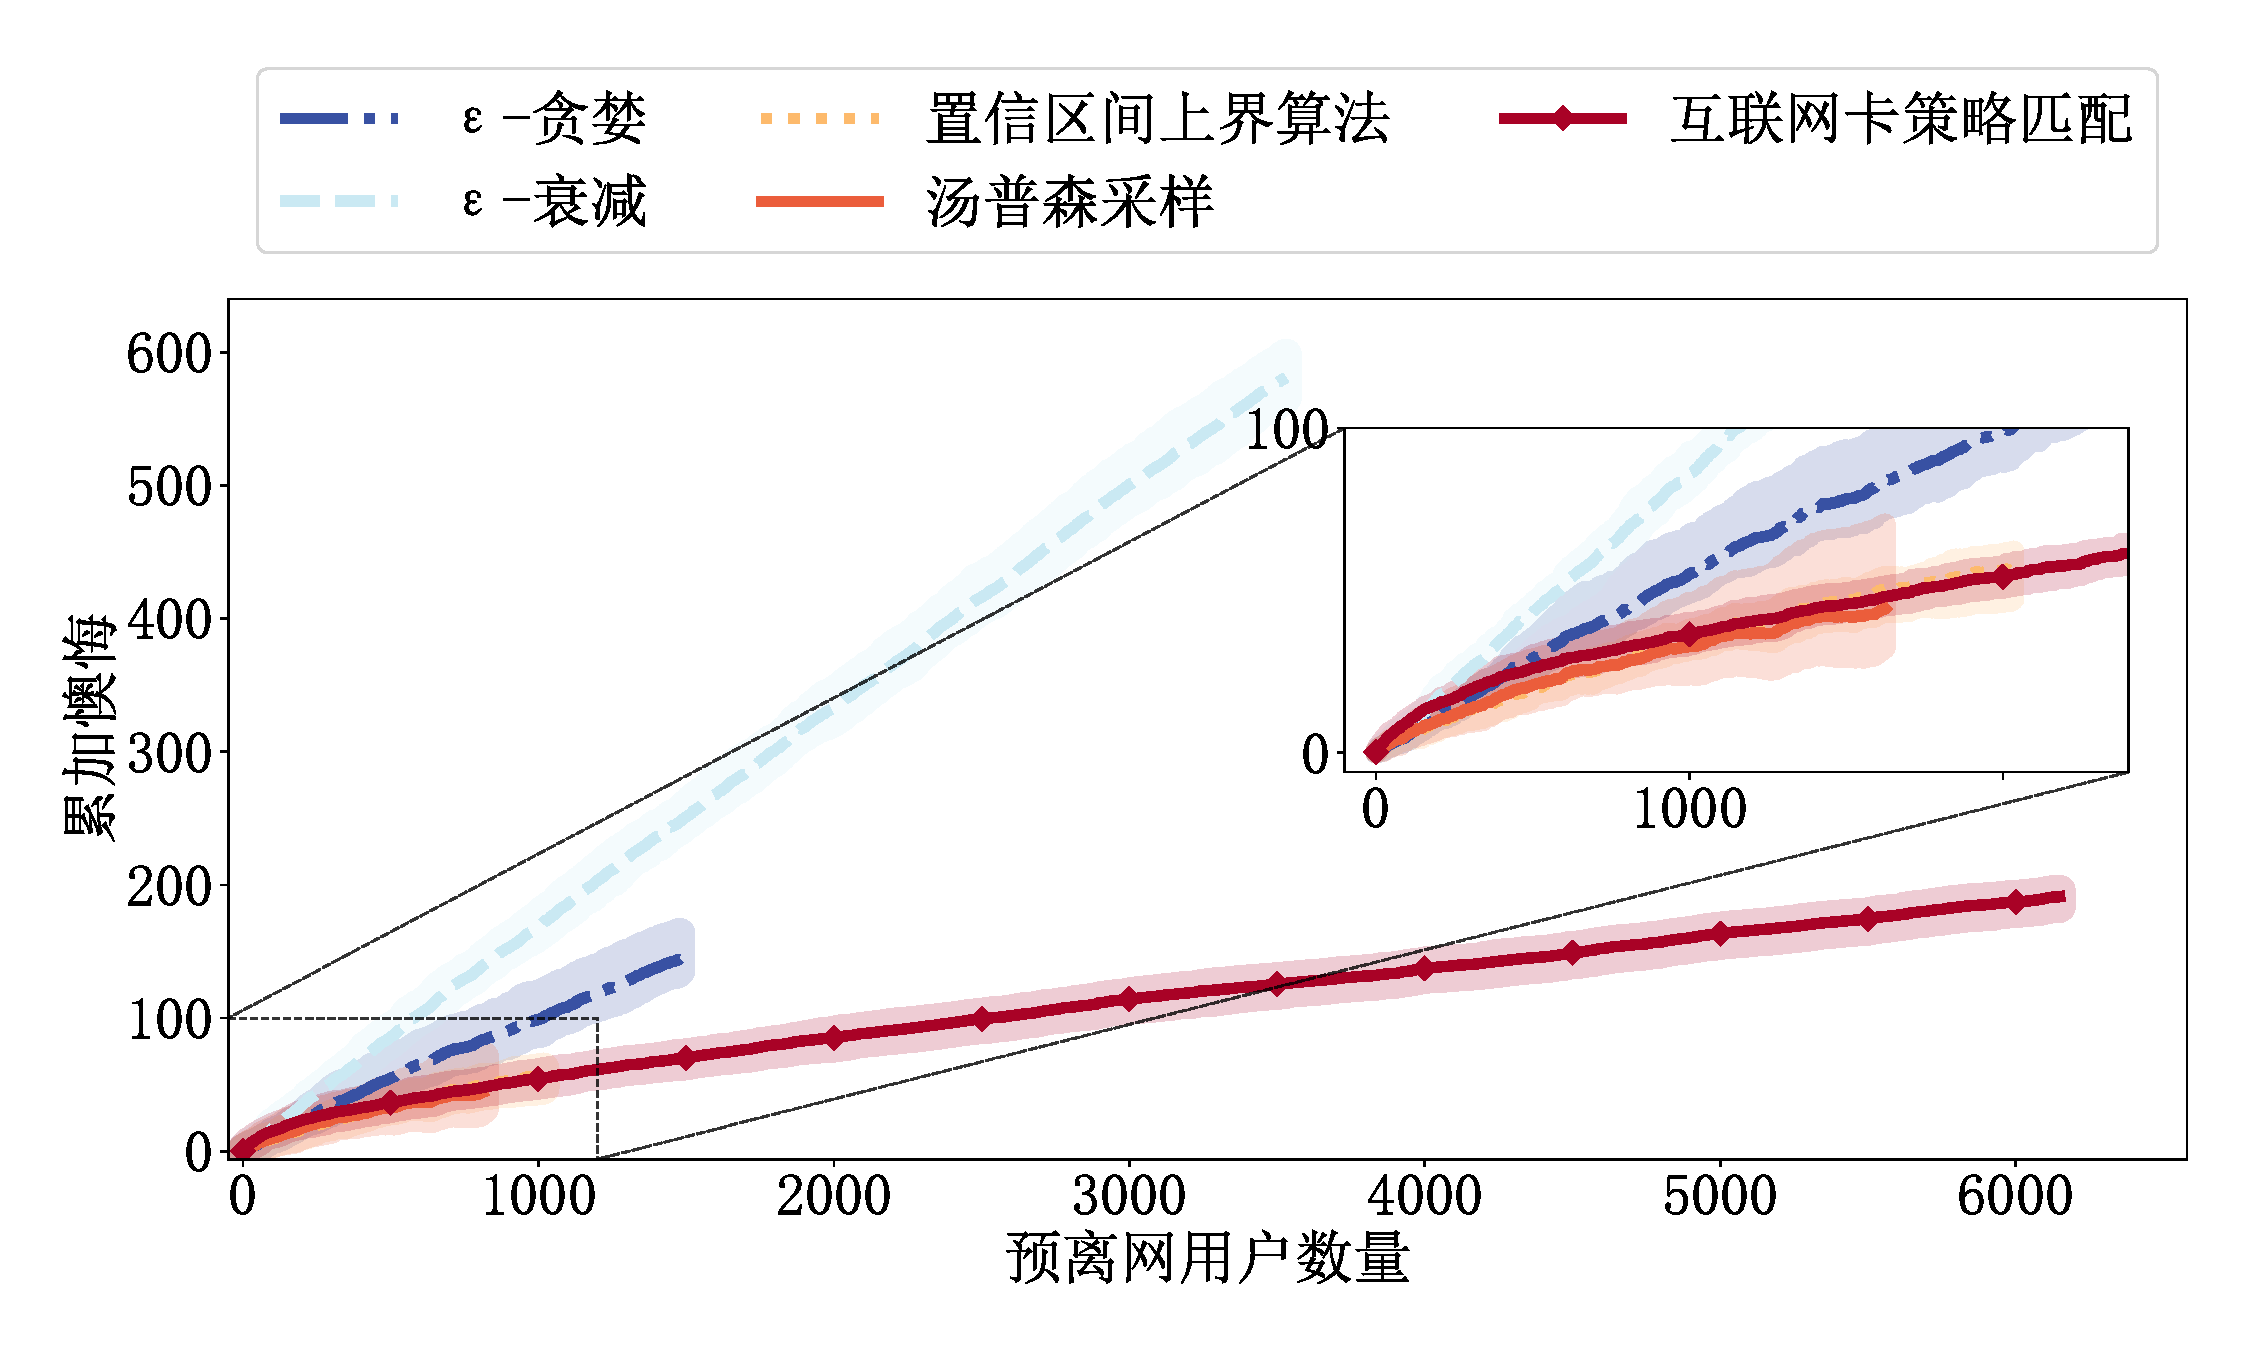
\includegraphics[width=1\textwidth]{Ms-ICSM_Exp-Perf-Cumulative-Regrets.pdf}
	\caption{匹配算法性能对比图}
	\label{Fig:Exp-Perf-Cumulative-Regrets}
\end{figure}
我们首先通过与基准匹配算法的比较来测试所提出的ICSM算法的性能。图\ref{Fig:Exp-Perf-Cumulative-Regrets}为5种不同匹配算法计算的累加懊悔值,实线表示5次独立实验下的平均性能,对应的面积表示性能的上下界。然后我们可以得到如下的表述。首先,我们提出的ICSM每轮累积遗憾次优只比TS差。同时,ICSM算法干预了最多的预离网用户,以获得与其他基准相比最好的奖励。第二,尽管TS和UCB在干预的初始阶段表现有效,但在干预的中期,由于预算不足,它们很快就失效了。它们沉迷于成功概率较高的策略,同时也付出了较高的代价。最后,观察$\epsilon$-贪婪算法和$\epsilon$-衰减算法,我们可以得出结论,这些算法更倾向于成功率叫低的策略,从而不能很好地挖掘干预策略的潜力。


\textbf{干预框架总体性能.}\par
\begin{figure}[hbt]
	\centering
	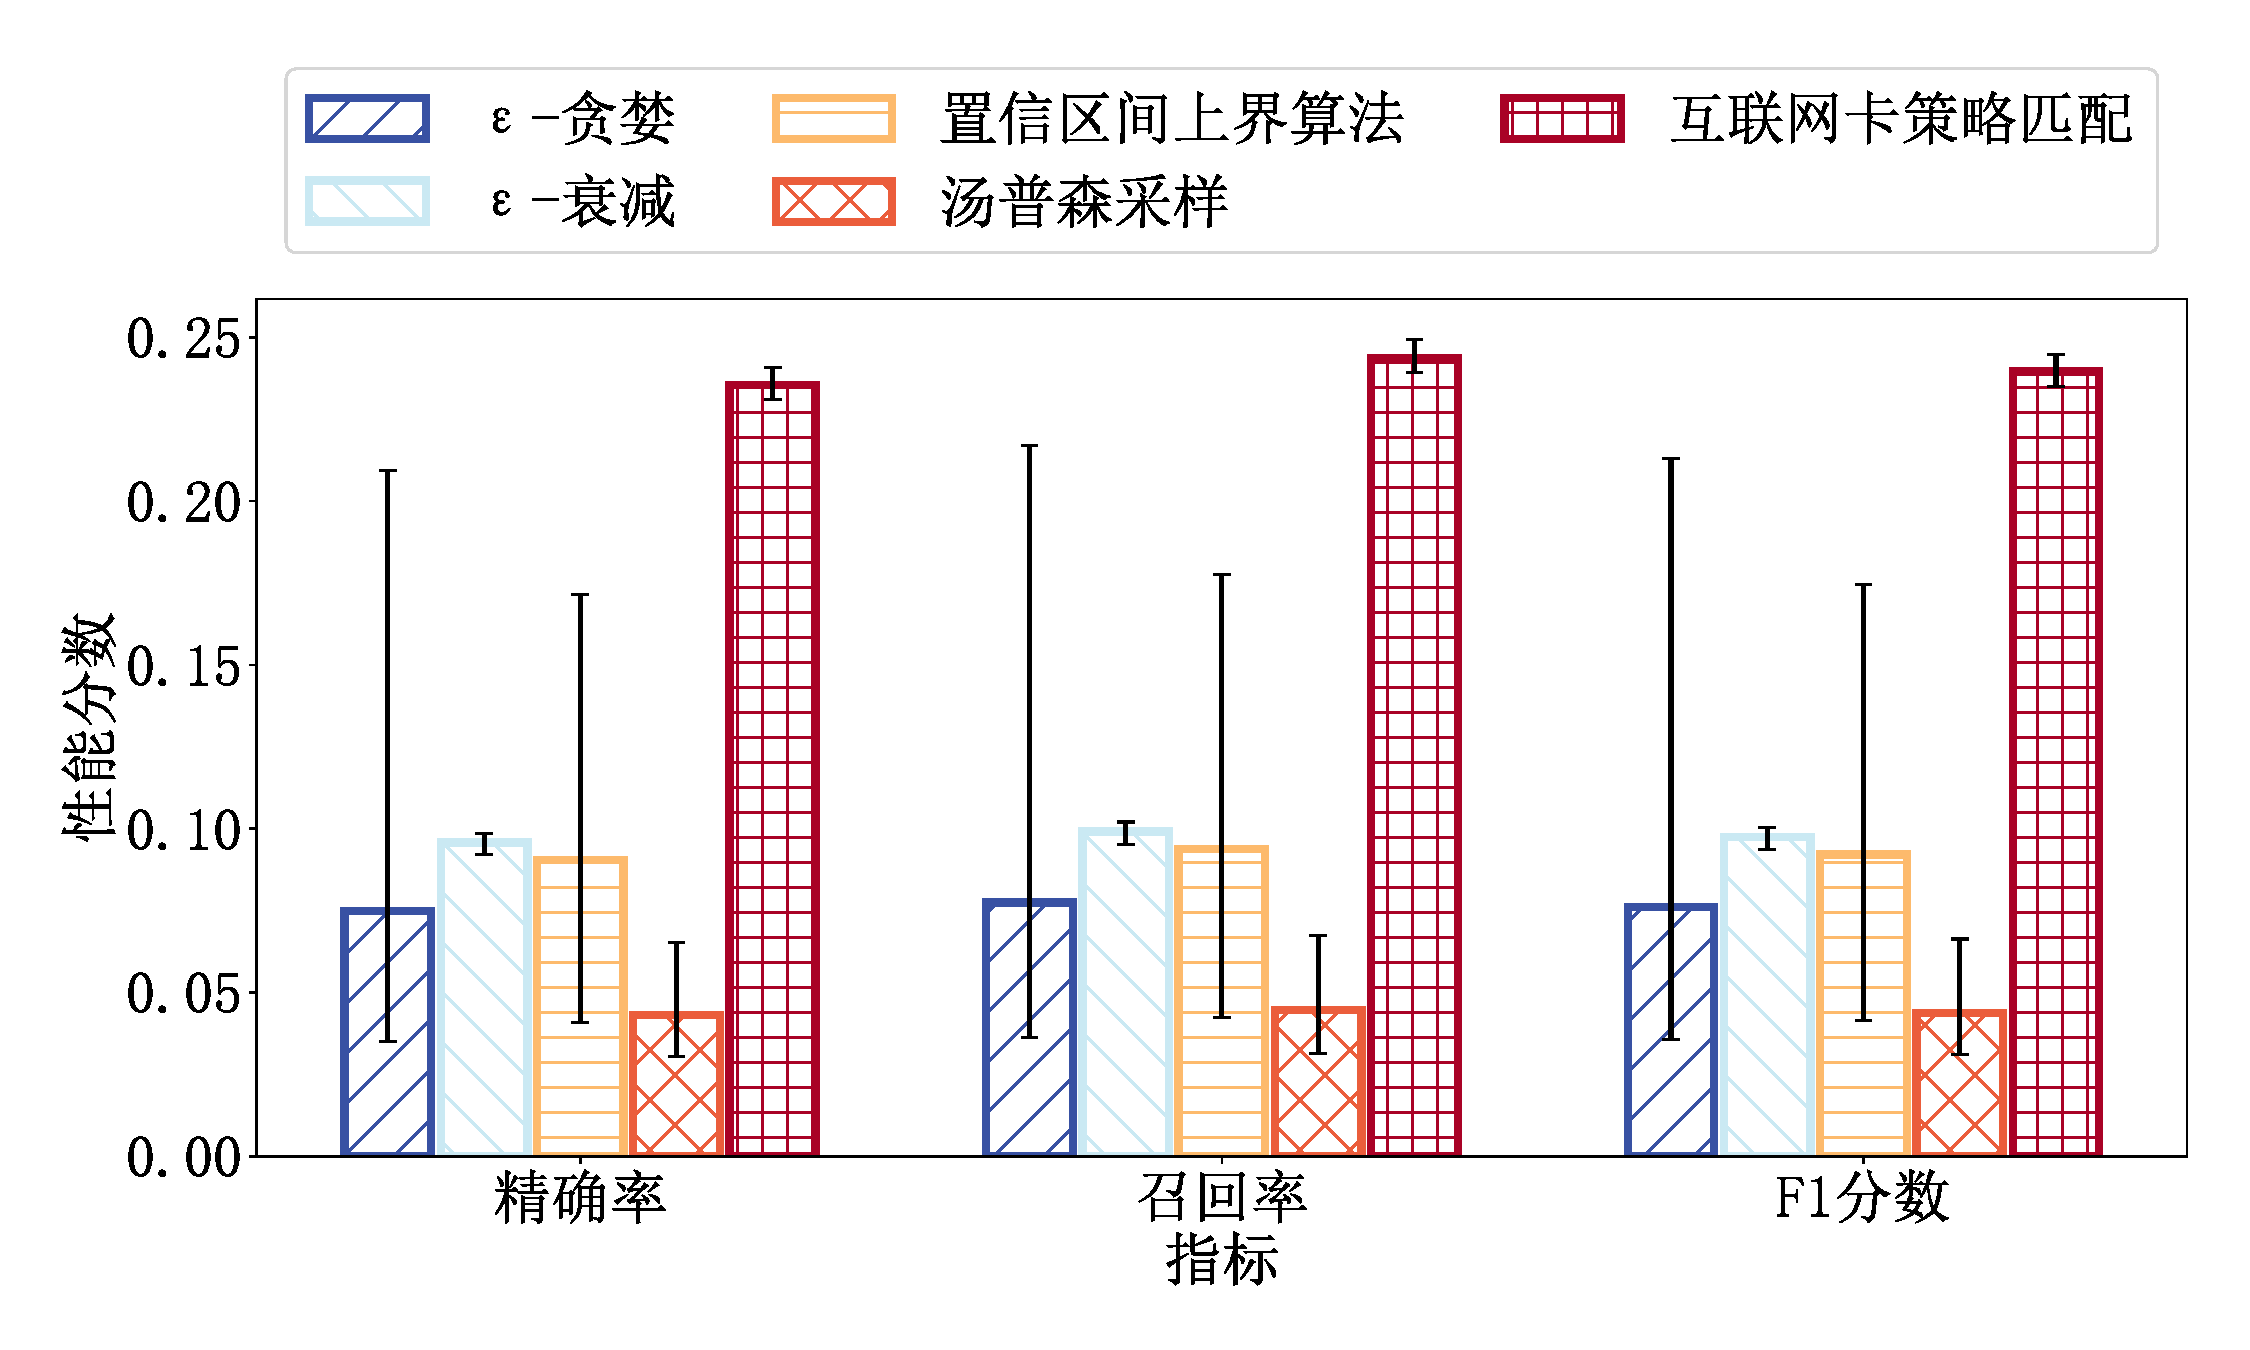
\includegraphics[width=1\textwidth]{Ms-ICSM_Exp-Perf-Classify.pdf}
	\caption{干预框架总体性能对比图}
	\label{Fig:Exp-Perf-Classify}
\end{figure}
为了证明我们提出的框架UPRS的优越性,我们检查了系统的整体性能,以评估整个工作流程的有效性,包括离网预测,偏好建模和策略匹配。因为被建模一个分类问题。因此,我们采用精准率、召回率和F1分数等指标来评估整体性能。图\ref{Fig:Exp-Perf-Classify}显示了各个匹配算法总体性能的平均值和上下界。我们可以进行如下的主要观察。首先,提出的ICSM算法在所有指标上都显著优于其他基准测试。例如,ICSM中精准率、召回率和F1分数的平均分数为{0.23,0.25,0.24},次优算法$\epsilon$-衰减的平均分约为{0.08,0.09,0.08}。其次是由于误差多重效应导致整体性能较低。具体来说,系统的整体性能取决于以下两个因素的乘积,一个是离网预测性能,另一个是干预策略匹配性能。



\textbf{商业指标.}


\begin{figure}[hbt]
	\centering
	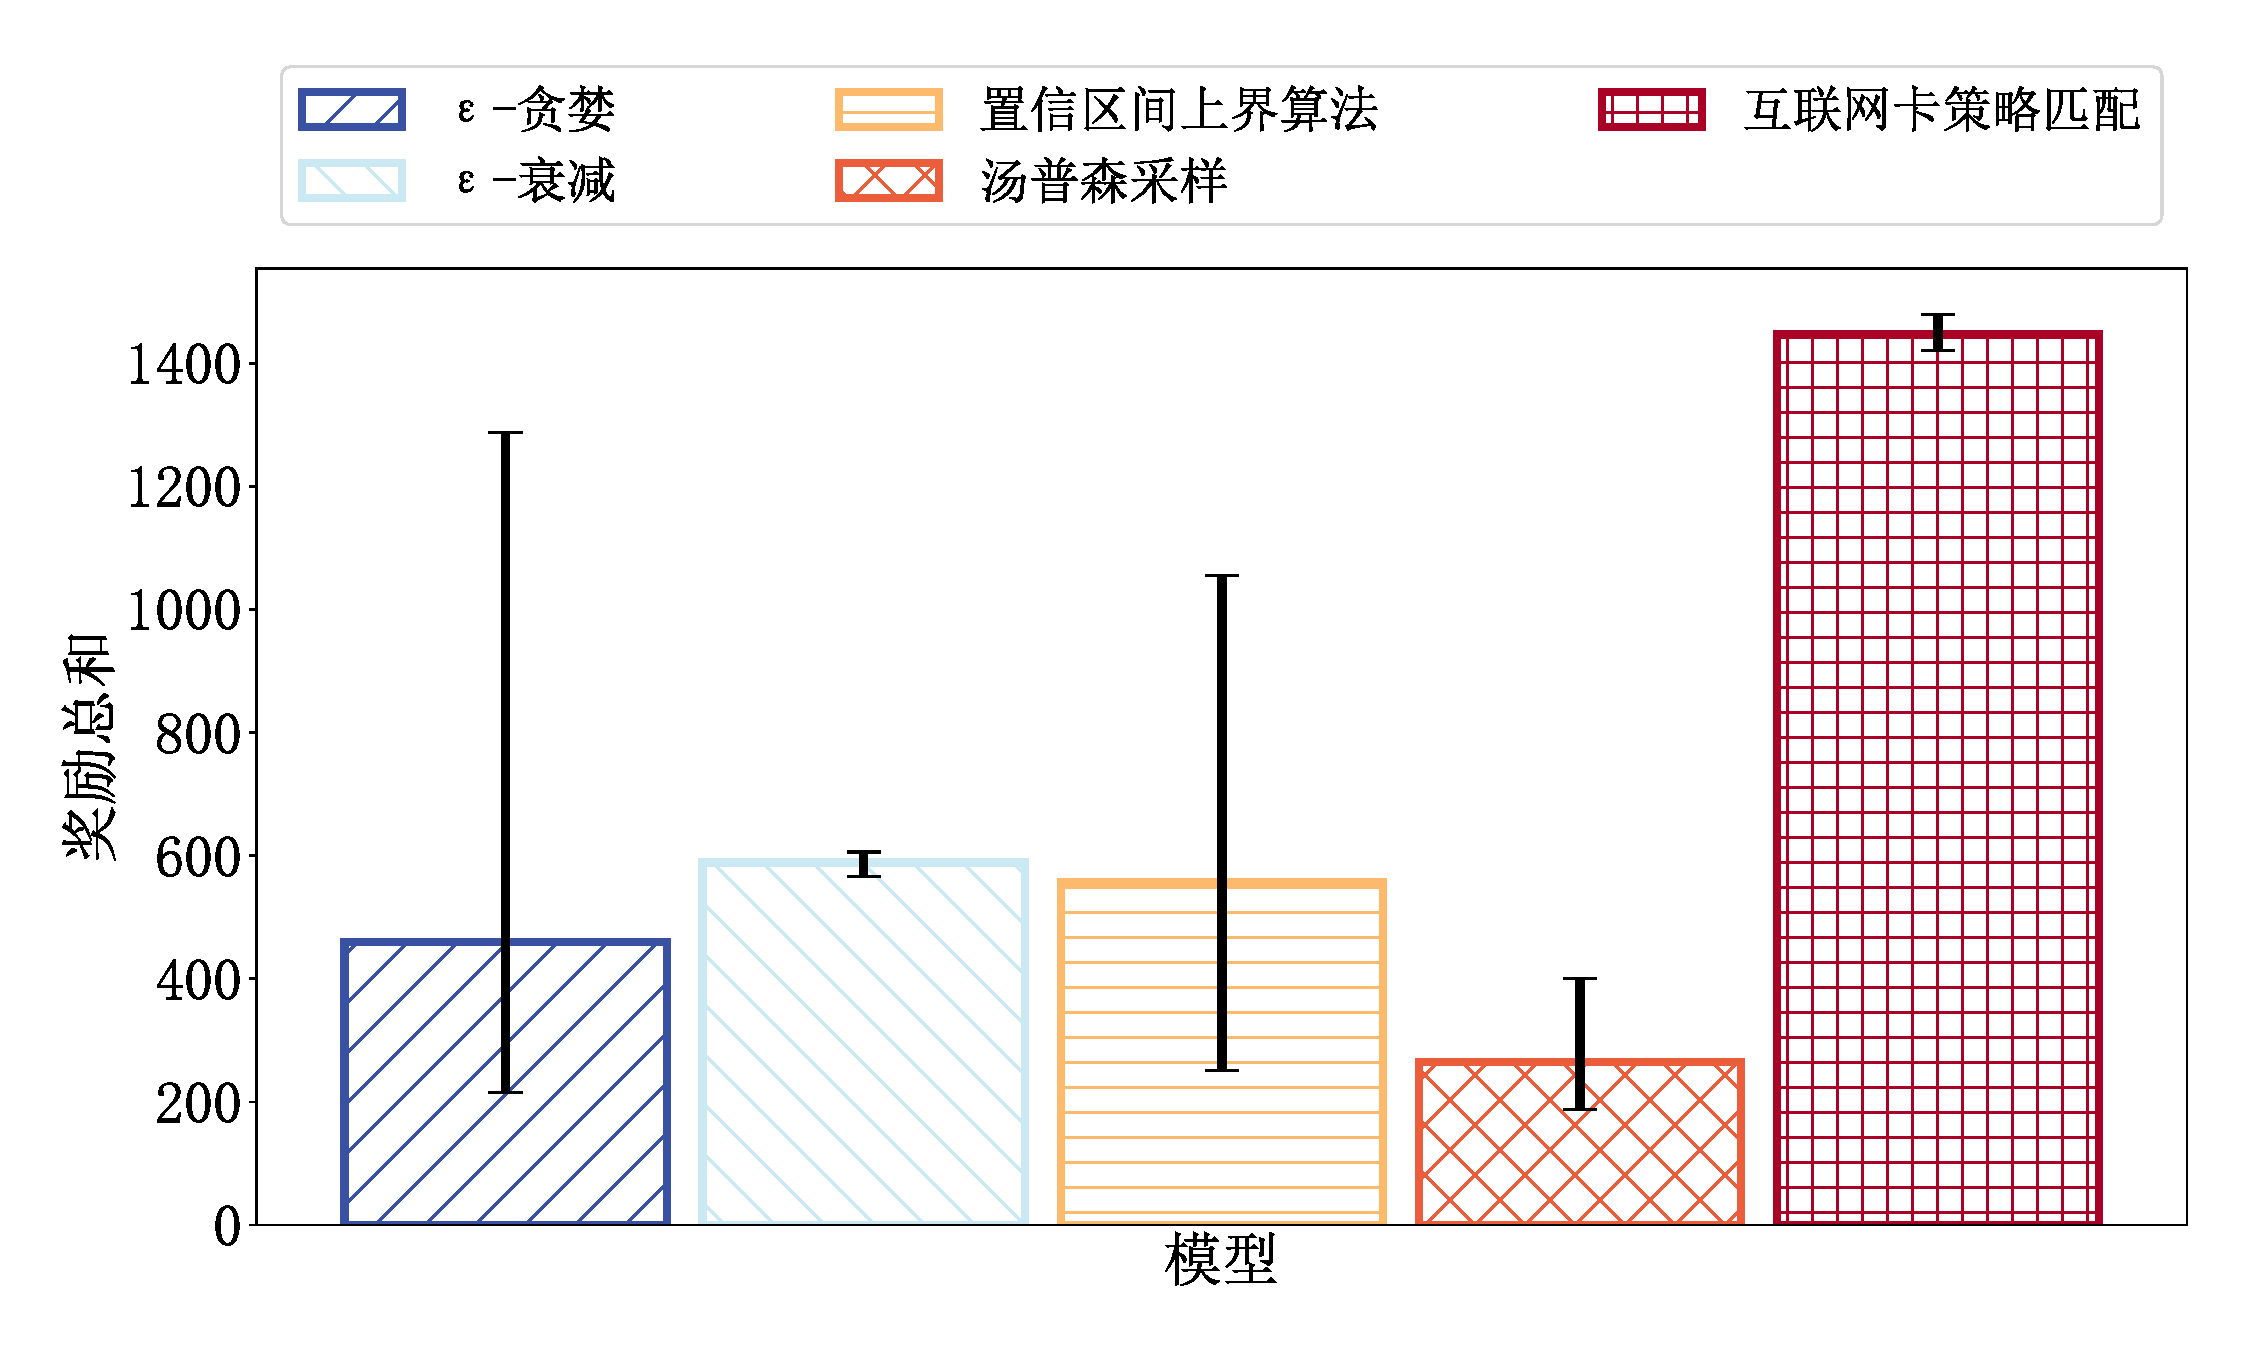
\includegraphics[width=1\textwidth]{Ms-ICSM_Exp-Perf-Business-Rewards.pdf}
	\caption{奖励总和对比图}
	\label{Fig:Exp-Perf-Business-Rewards}
\end{figure}

\begin{figure}[hbt]
	\centering
	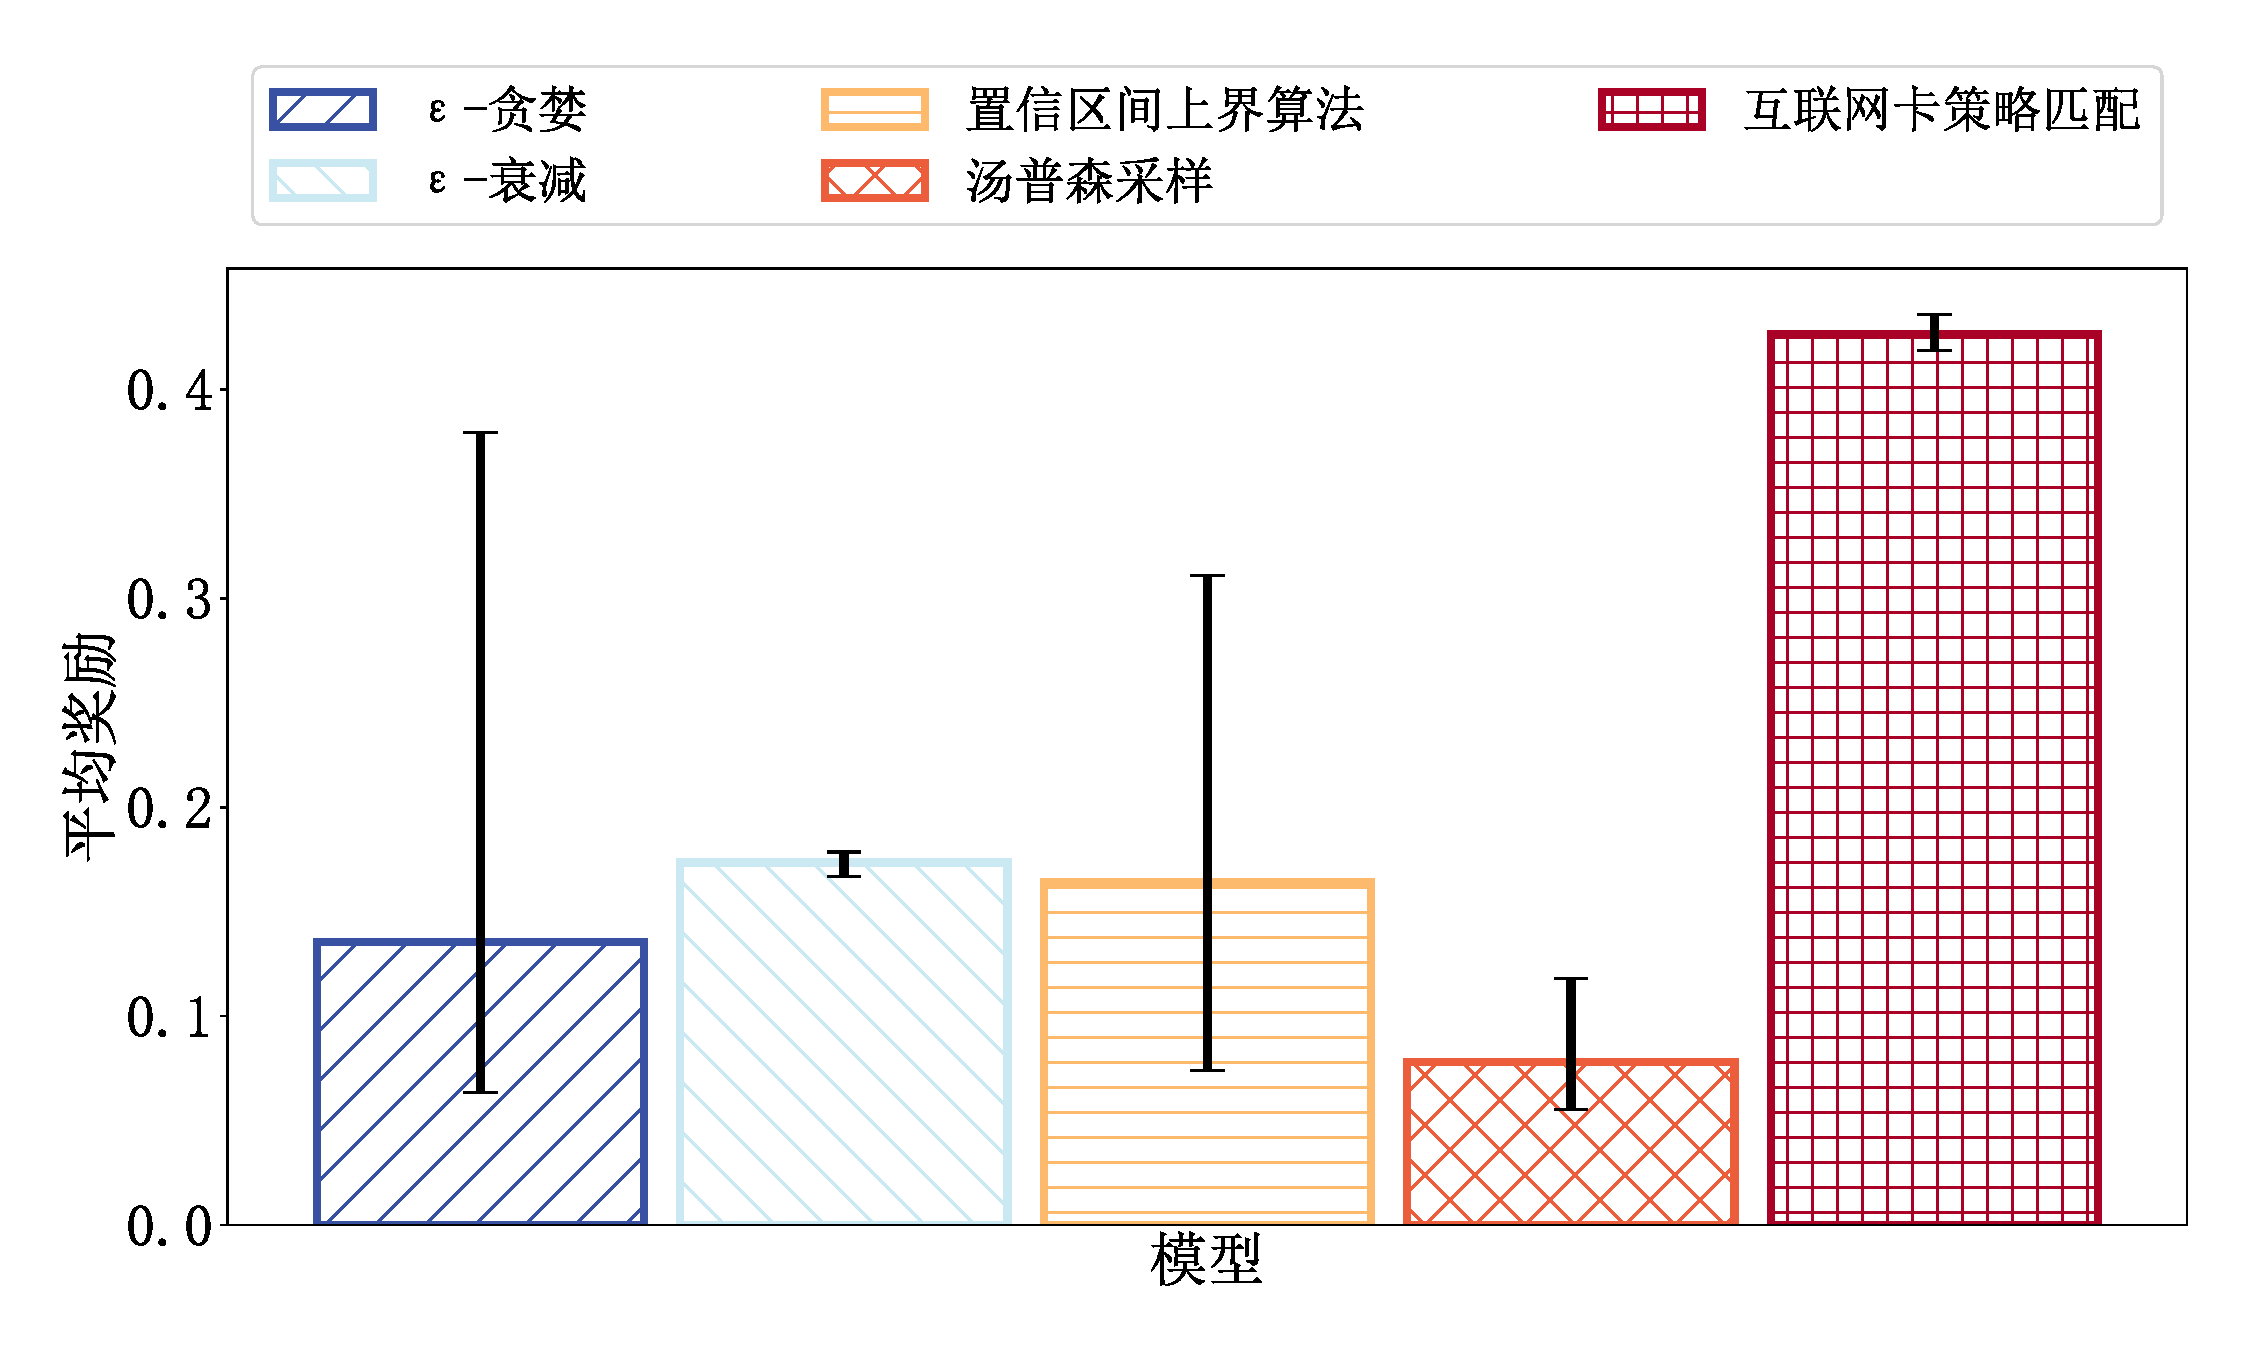
\includegraphics[width=1\textwidth]{Ms-ICSM_Exp-Perf-Business-Average_Reward.pdf}
	\caption{平均奖励对比图}
	\label{Fig:Exp-Perf-Business-Average_Reward}
\end{figure}

\begin{figure}[hbt]
	\centering
	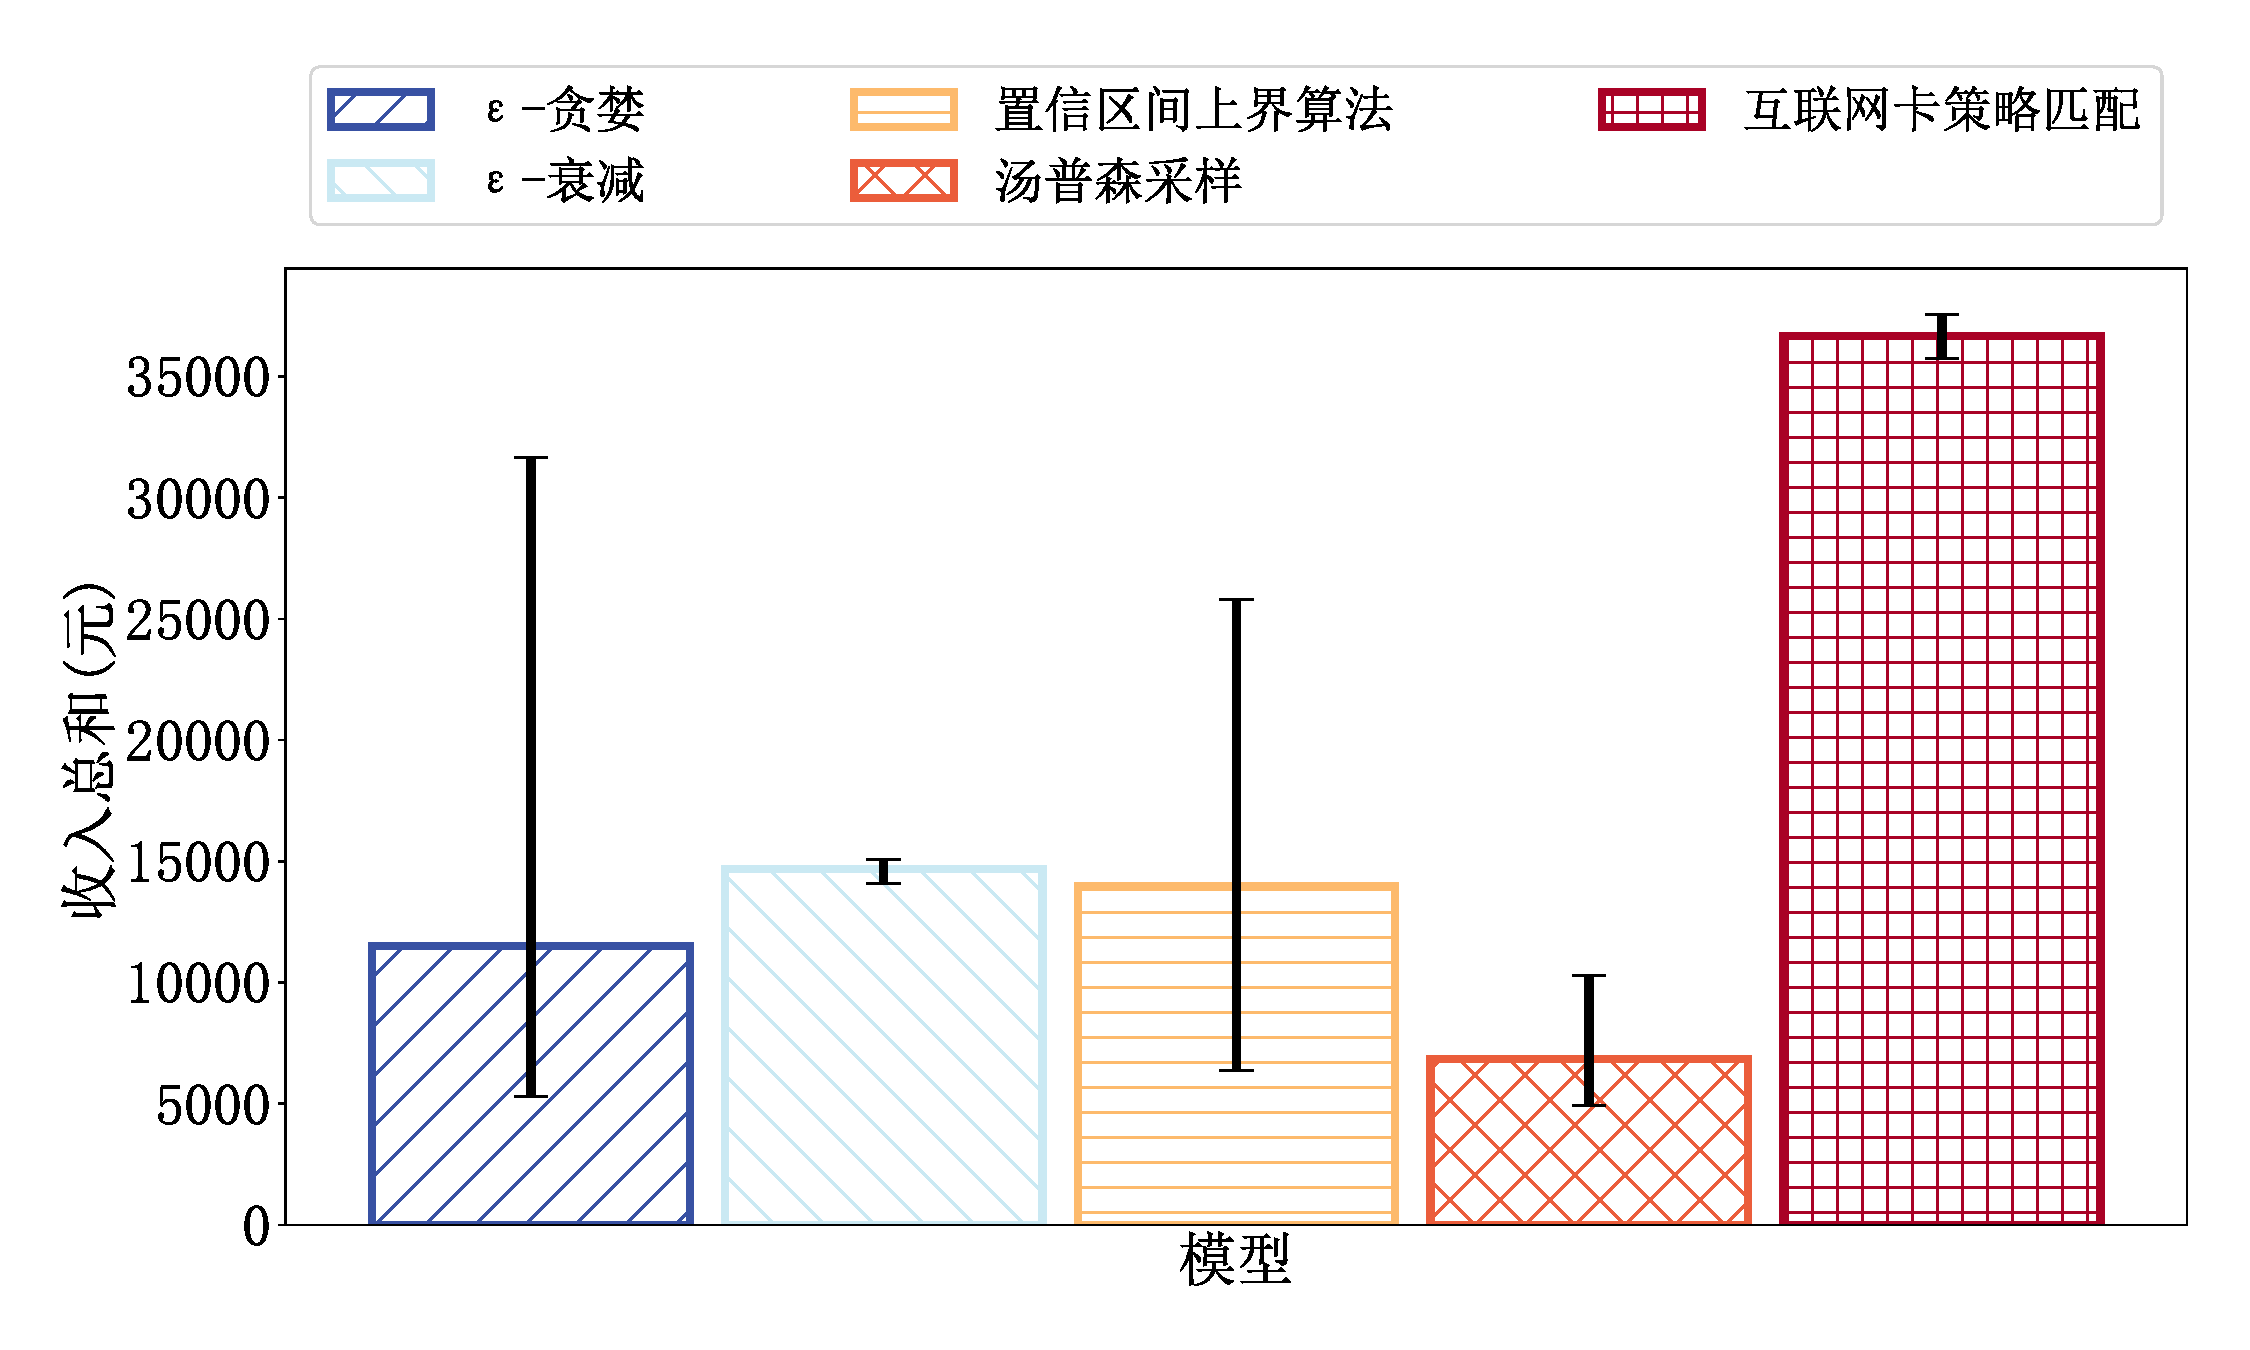
\includegraphics[width=1\textwidth]{Ms-ICSM_Exp-Perf-Business-Total_Revenue.pdf}
	\caption{收入总和对比图}
	\label{Fig:Exp-Perf-Business-Total_Revenue}
\end{figure}




我们选择了三个典型的业务指标来证明所提出的框架的有效性,分别是奖励总和、平均奖励和收入总和。根据图\ref{Fig:Exp-Perf-Business-Average_Reward},我们可以得出以下结论。首先,我们可以看到ICSM在三个指标上优于所有基线算法。其中,$\epsilon$-贪婪、$\epsilon$-衰减、置信区间上界算法、汤普森采样的平均奖励的平均得分分别为0.12、0.16、0.13、0.11, ICSM的平均奖励平均得分为0.41,性能分别提高了242\%、156\%、215\%、273\%。其次,本文提出的ICSM算法在5个独立实验中表现出相当的稳定性,总体性能波动仅为1\%,有利于在工业生产环境中部署。







\subsubsection{健壮性测试}
在评估了我们提出的框架的总体性能后,超参数、用户特征如何影响整个系统的健壮性是我们感兴趣的。因此,我们进行了以下参数影响实验。
%After evaluating the general performance of our proposed framework, how the hyper parameters, user characteristics
%effect the robustness of whole system is of interest to us. Therefore, we conduct the following impact experiments.


\begin{figure}[!htb]
	\centering
	\begin{subfigure}[t]{0.99\linewidth}
		\captionsetup{justification=centering} %子图caption居中
		\begin{minipage}[b]{1\linewidth}
			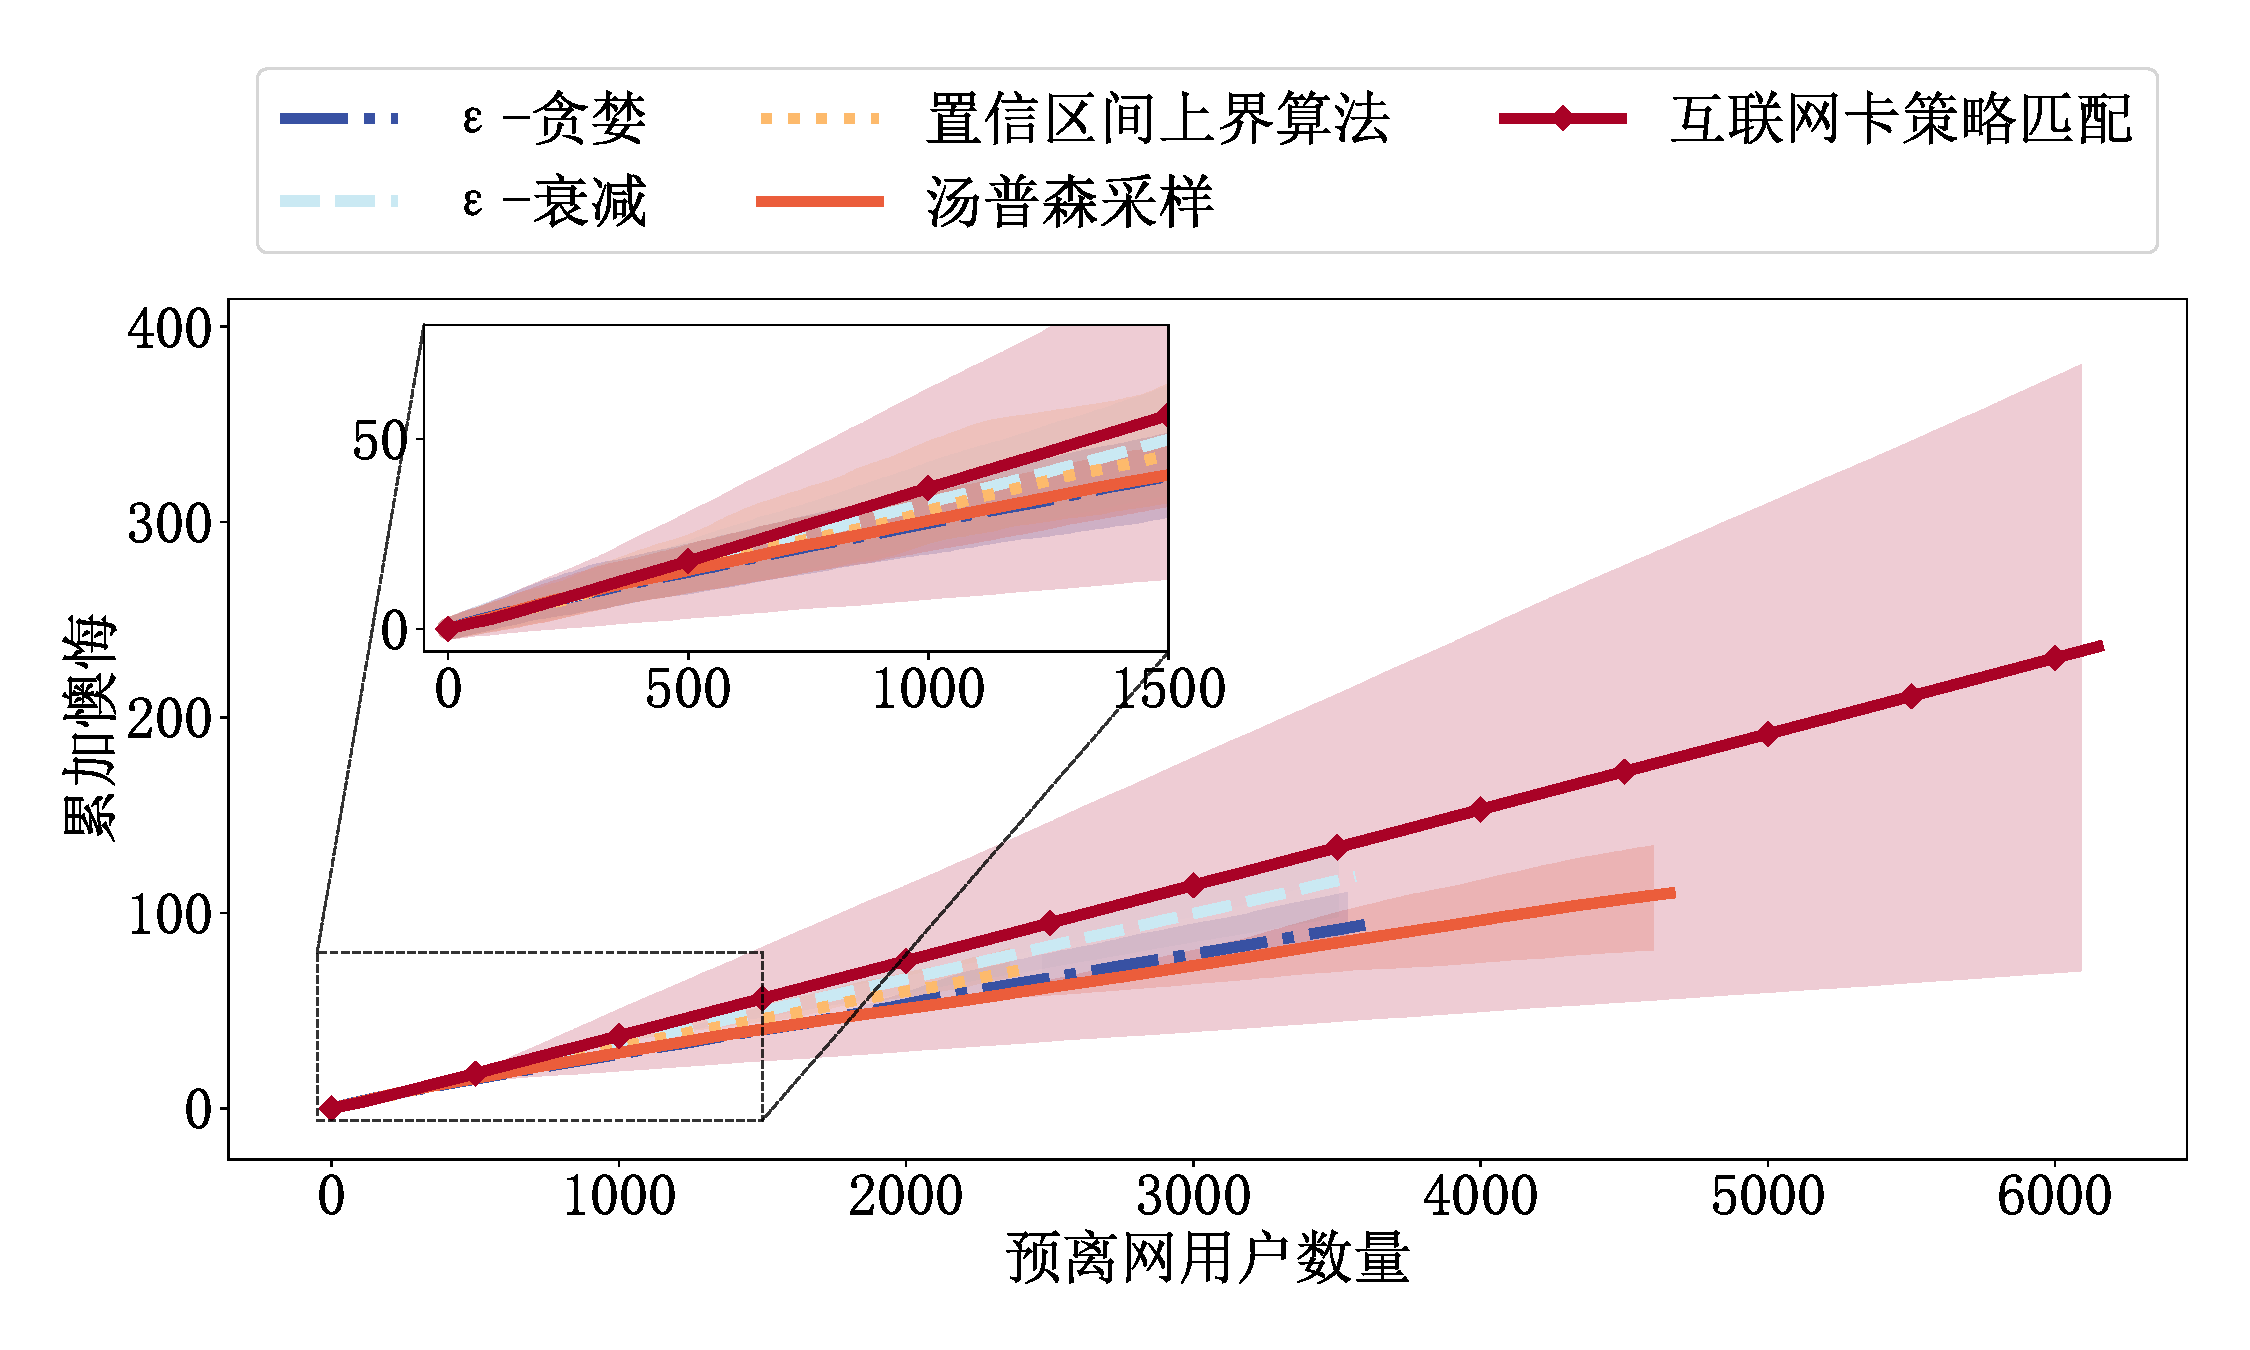
\includegraphics[width=0.49\linewidth]{Ms-ICSM_Exp-Imp-Cumulative-Regrets-Binomial.pdf}
			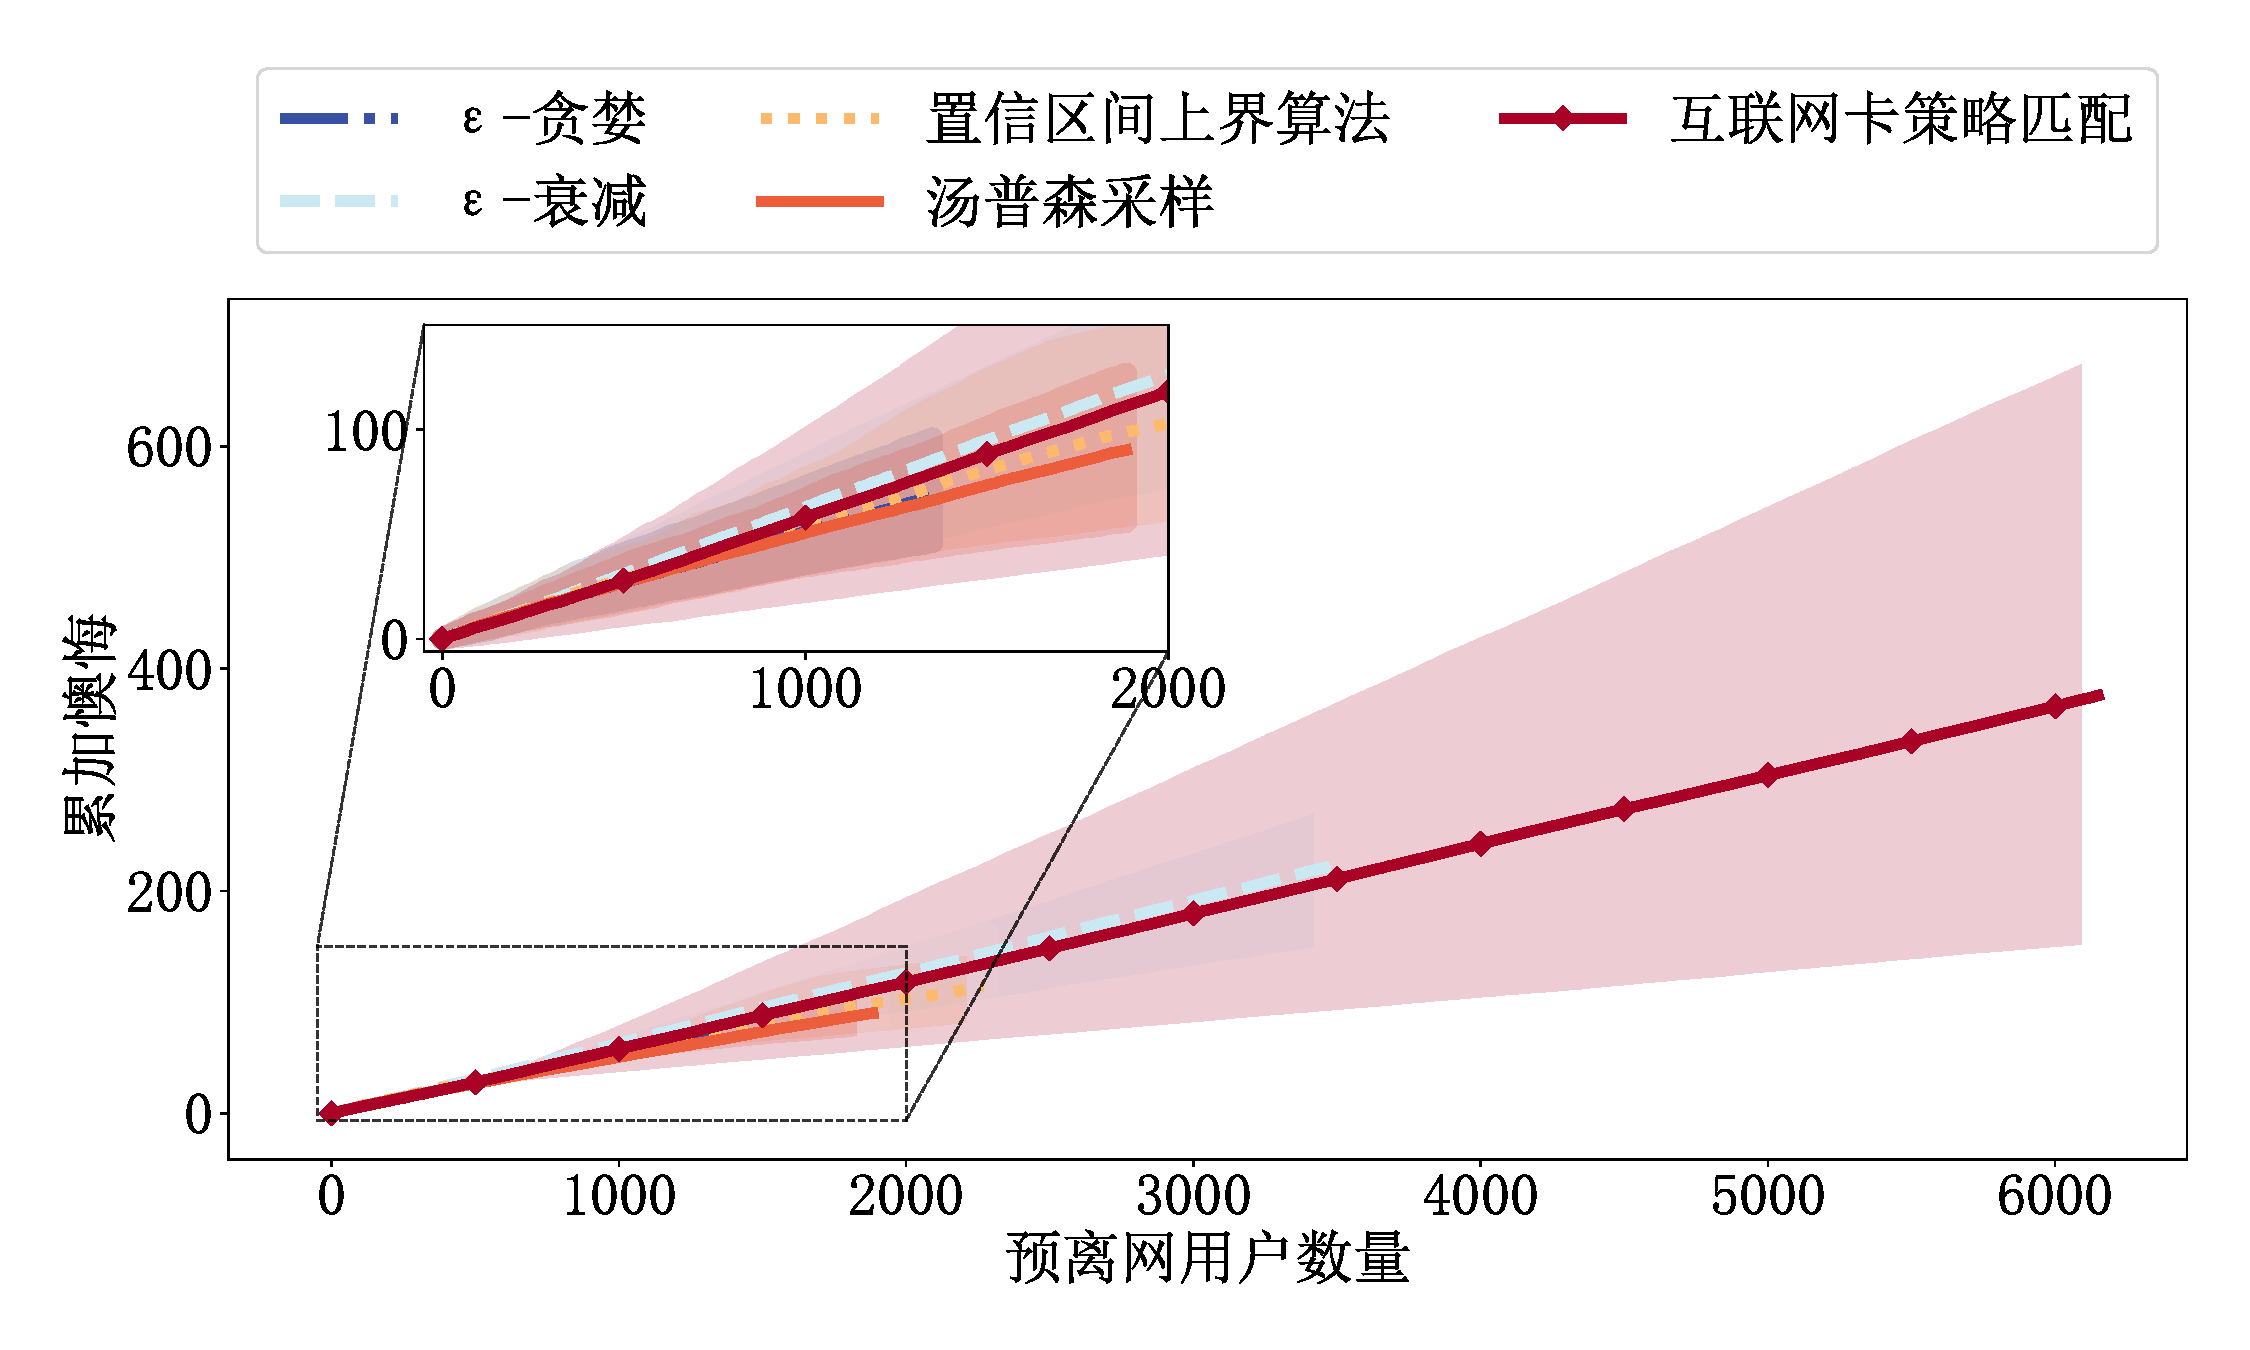
\includegraphics[width=0.49\linewidth]{Ms-ICSM_Exp-Imp-Cumulative-Regrets-Gaussian.pdf}
			\caption{二项式分布\&高斯分布}
		\end{minipage}
	\end{subfigure}\\	
	\begin{subfigure}[t]{0.99\linewidth}
		\captionsetup{justification=centering} %子图caption居中
		\begin{minipage}[b]{1\linewidth}
			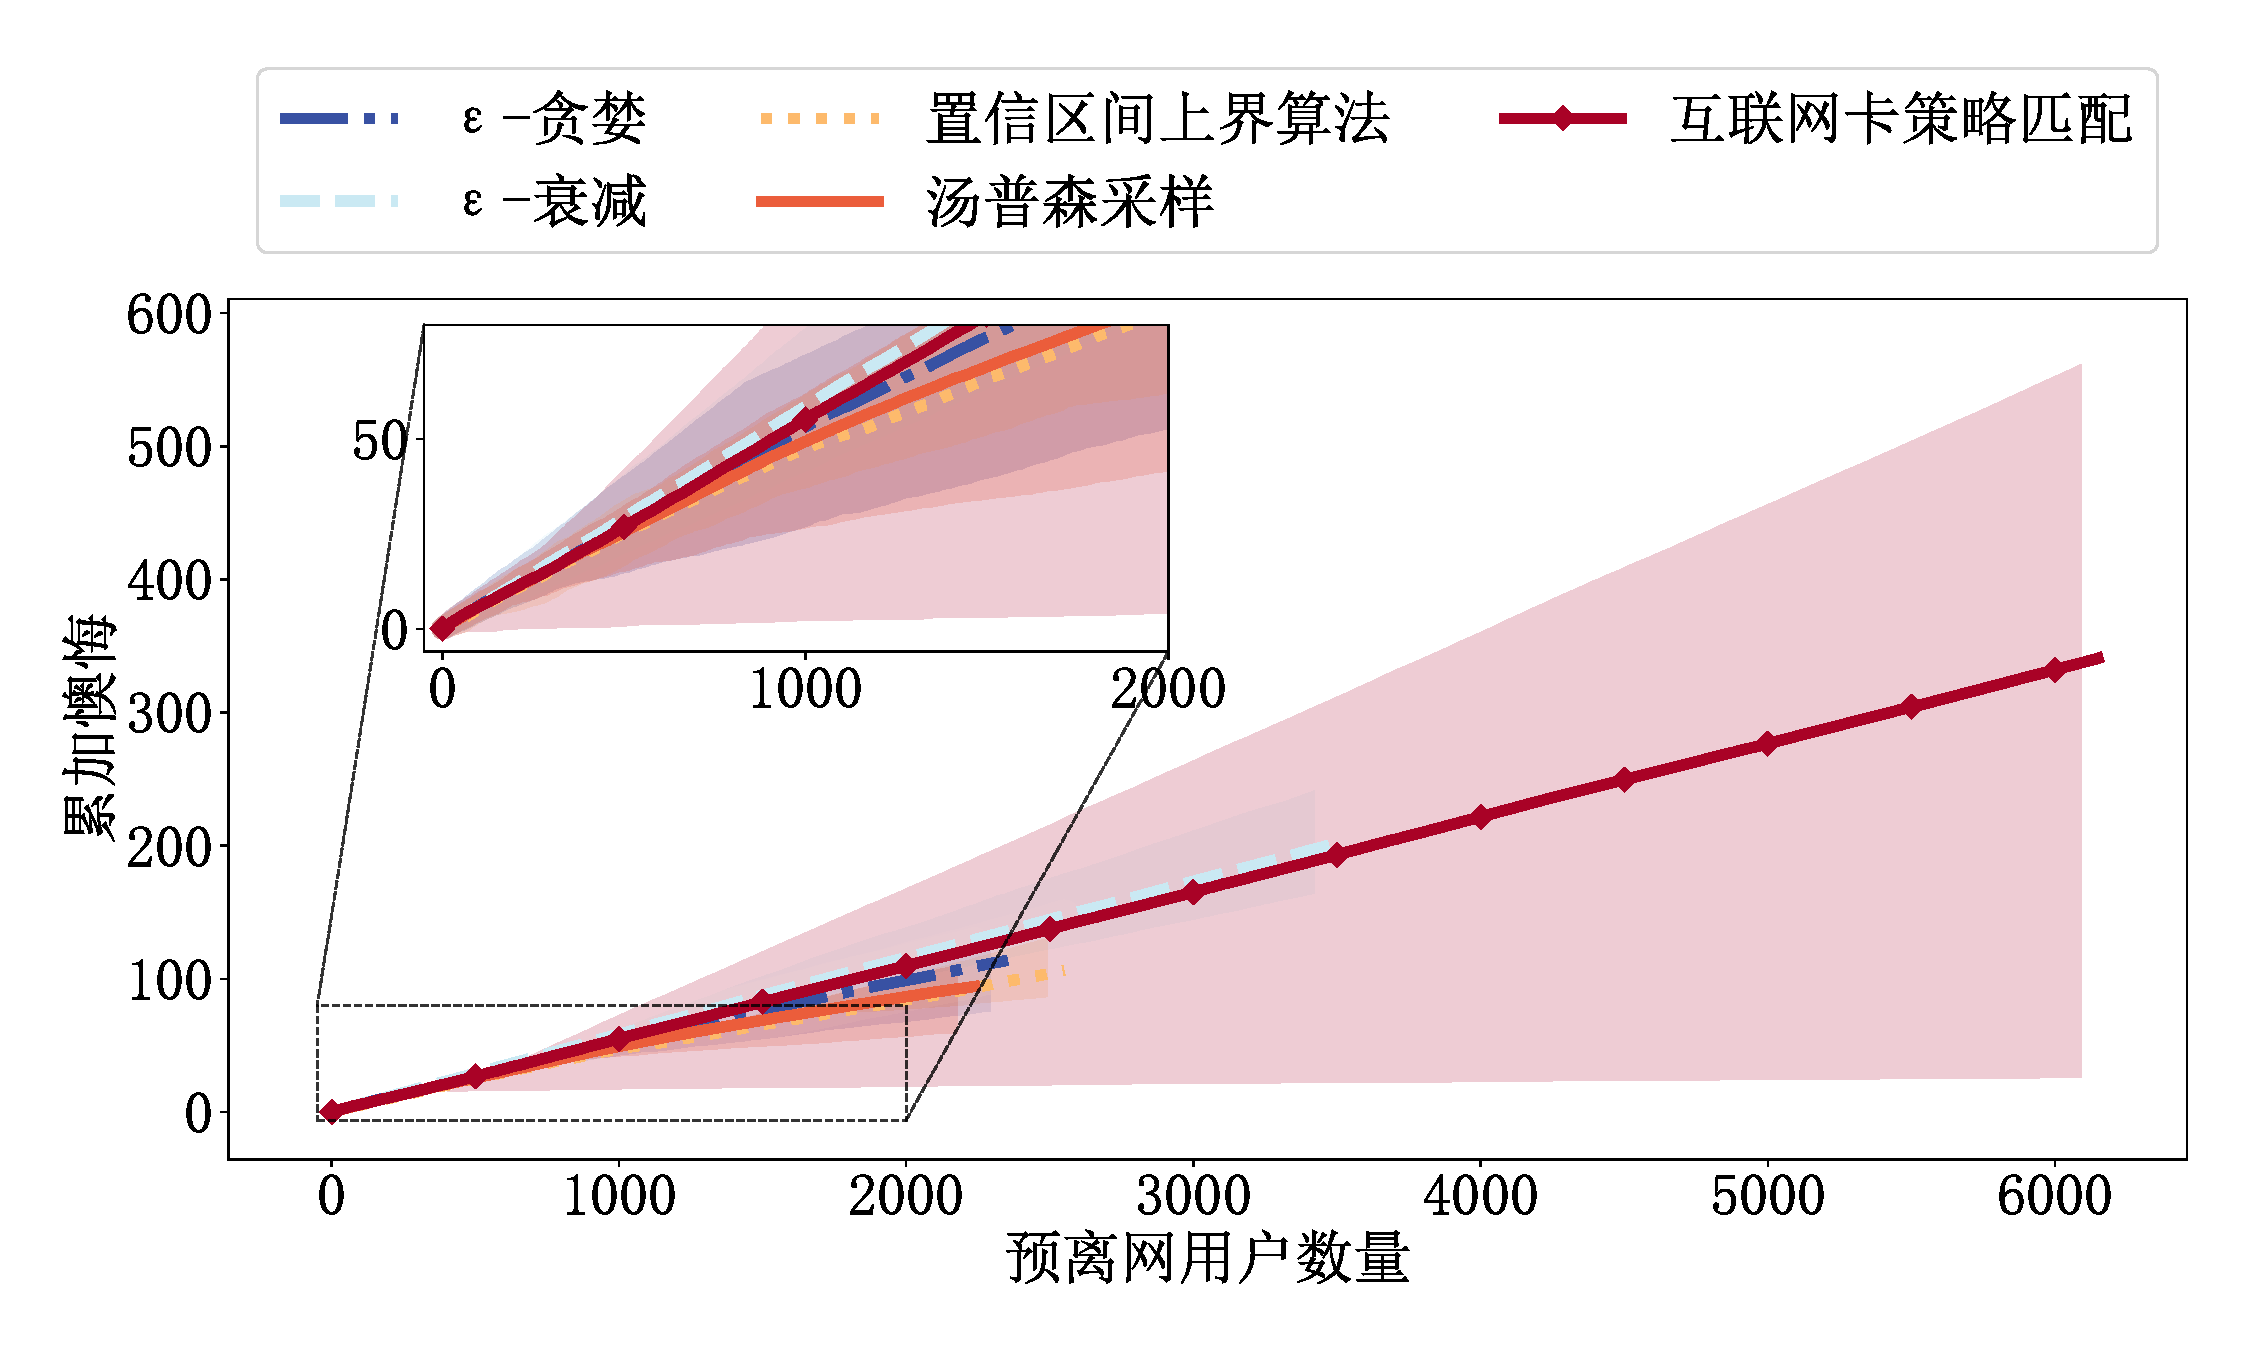
\includegraphics[width=0.49\linewidth]{Ms-ICSM_Exp-Imp-Cumulative-Regrets-Poisson.pdf}
			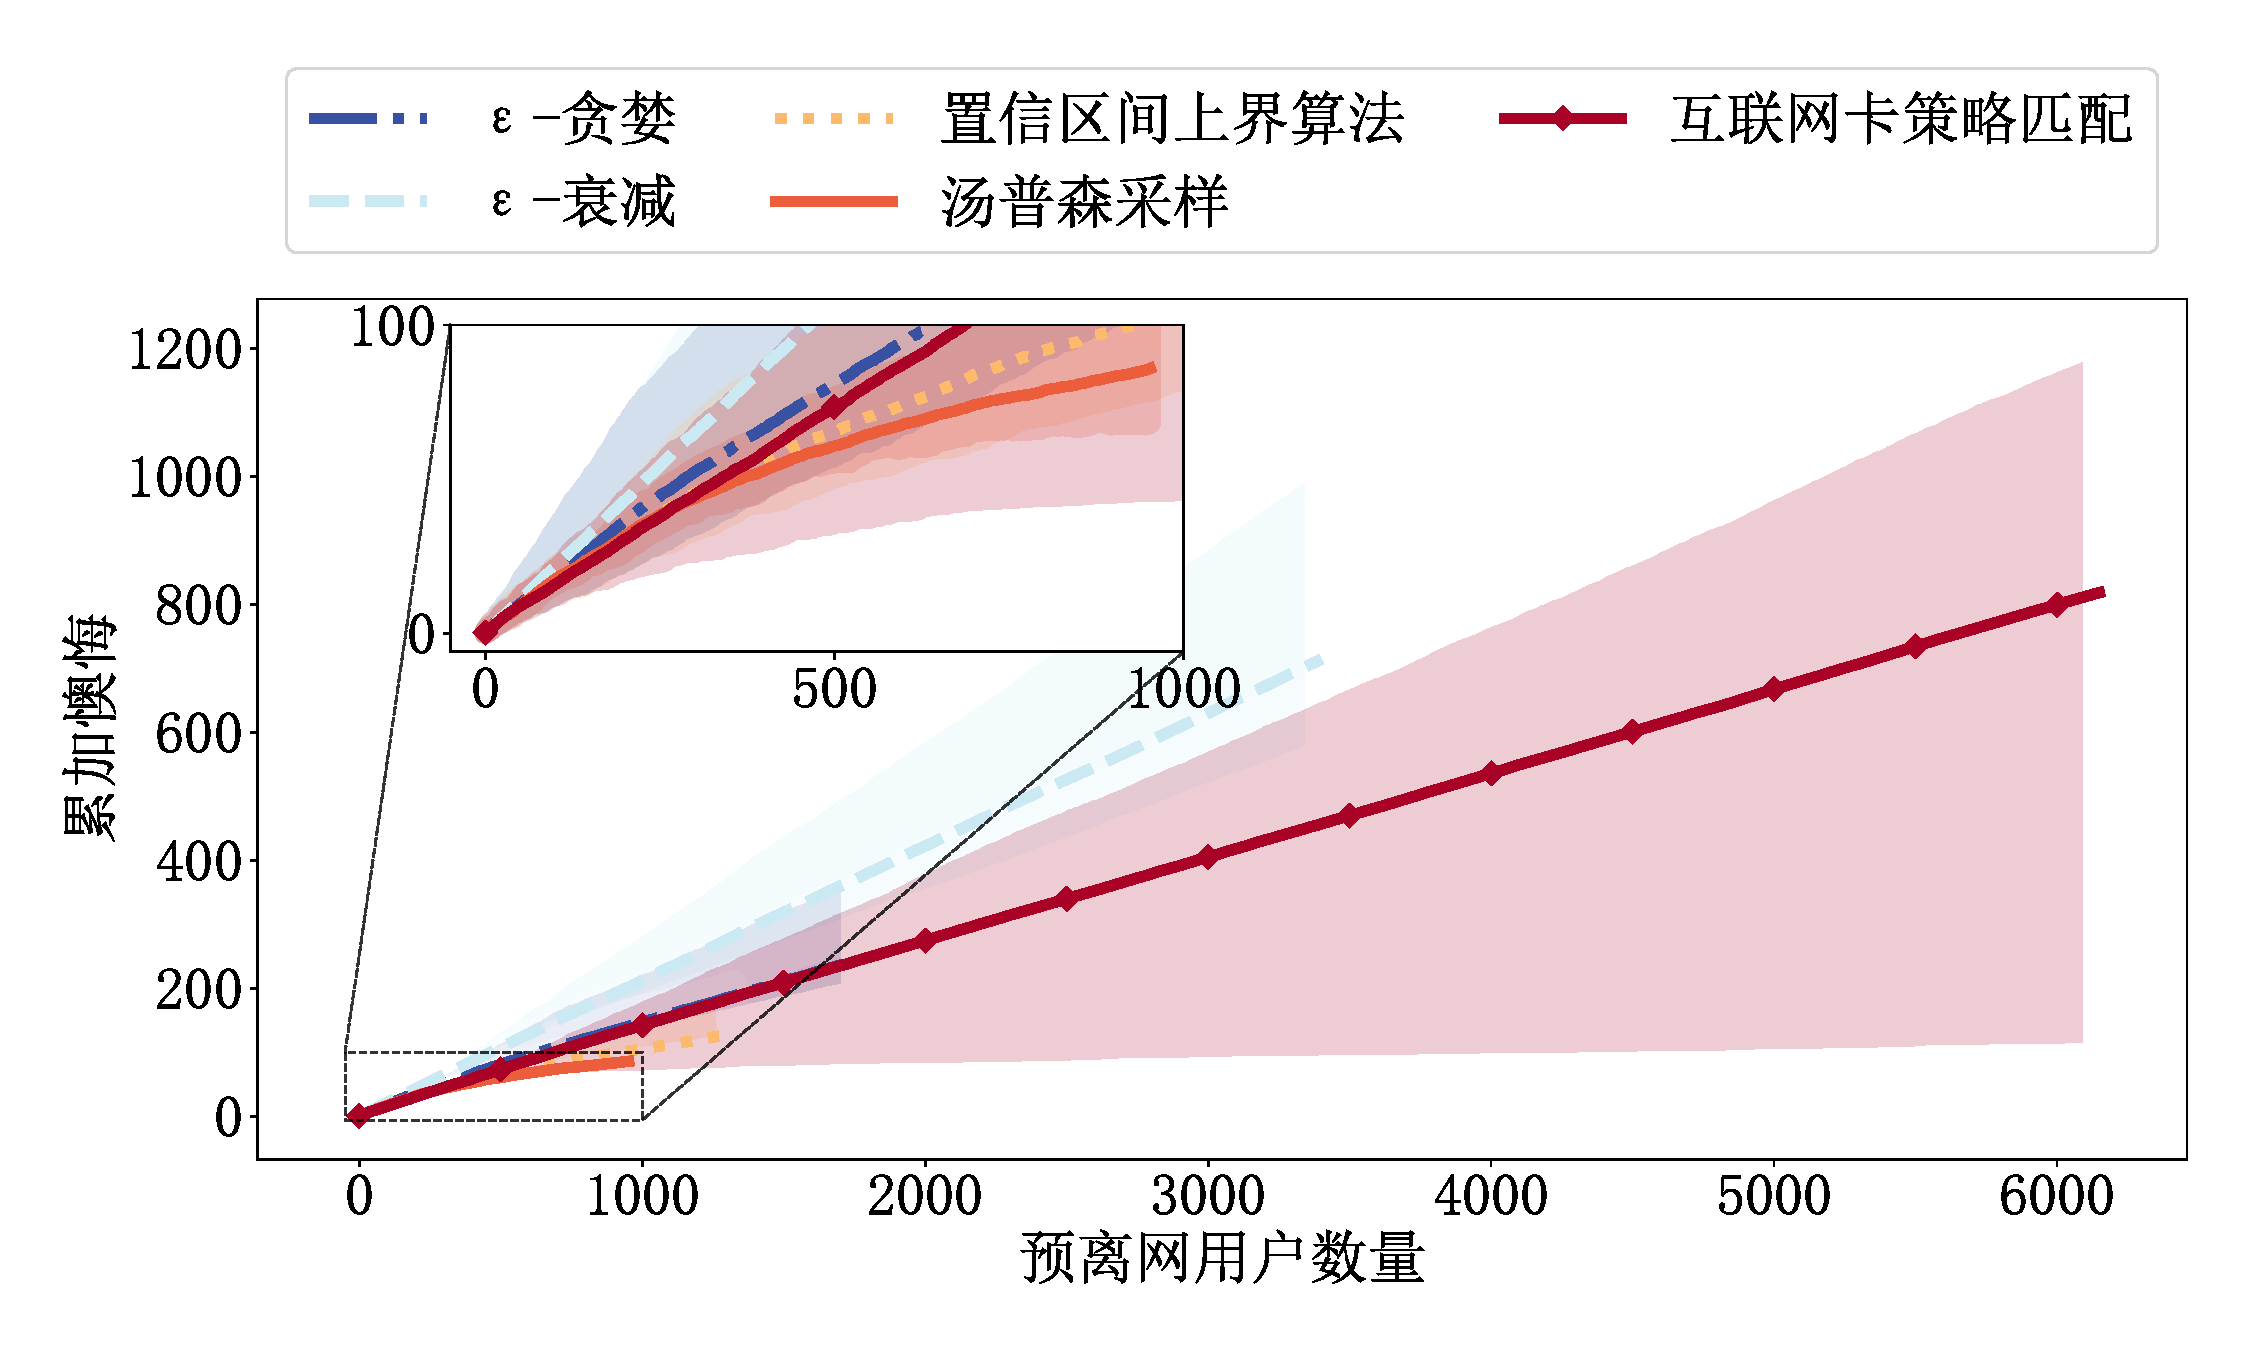
\includegraphics[width=0.49\linewidth]{Ms-ICSM_Exp-Imp-Cumulative-Regrets-Gamma.pdf}
			\caption{泊松分布\&伽马分布}
		\end{minipage}
	\end{subfigure}\\
	\begin{subfigure}[t]{0.99\linewidth}
		\captionsetup{justification=centering} %子图caption居中
		\begin{minipage}[b]{1\linewidth}
			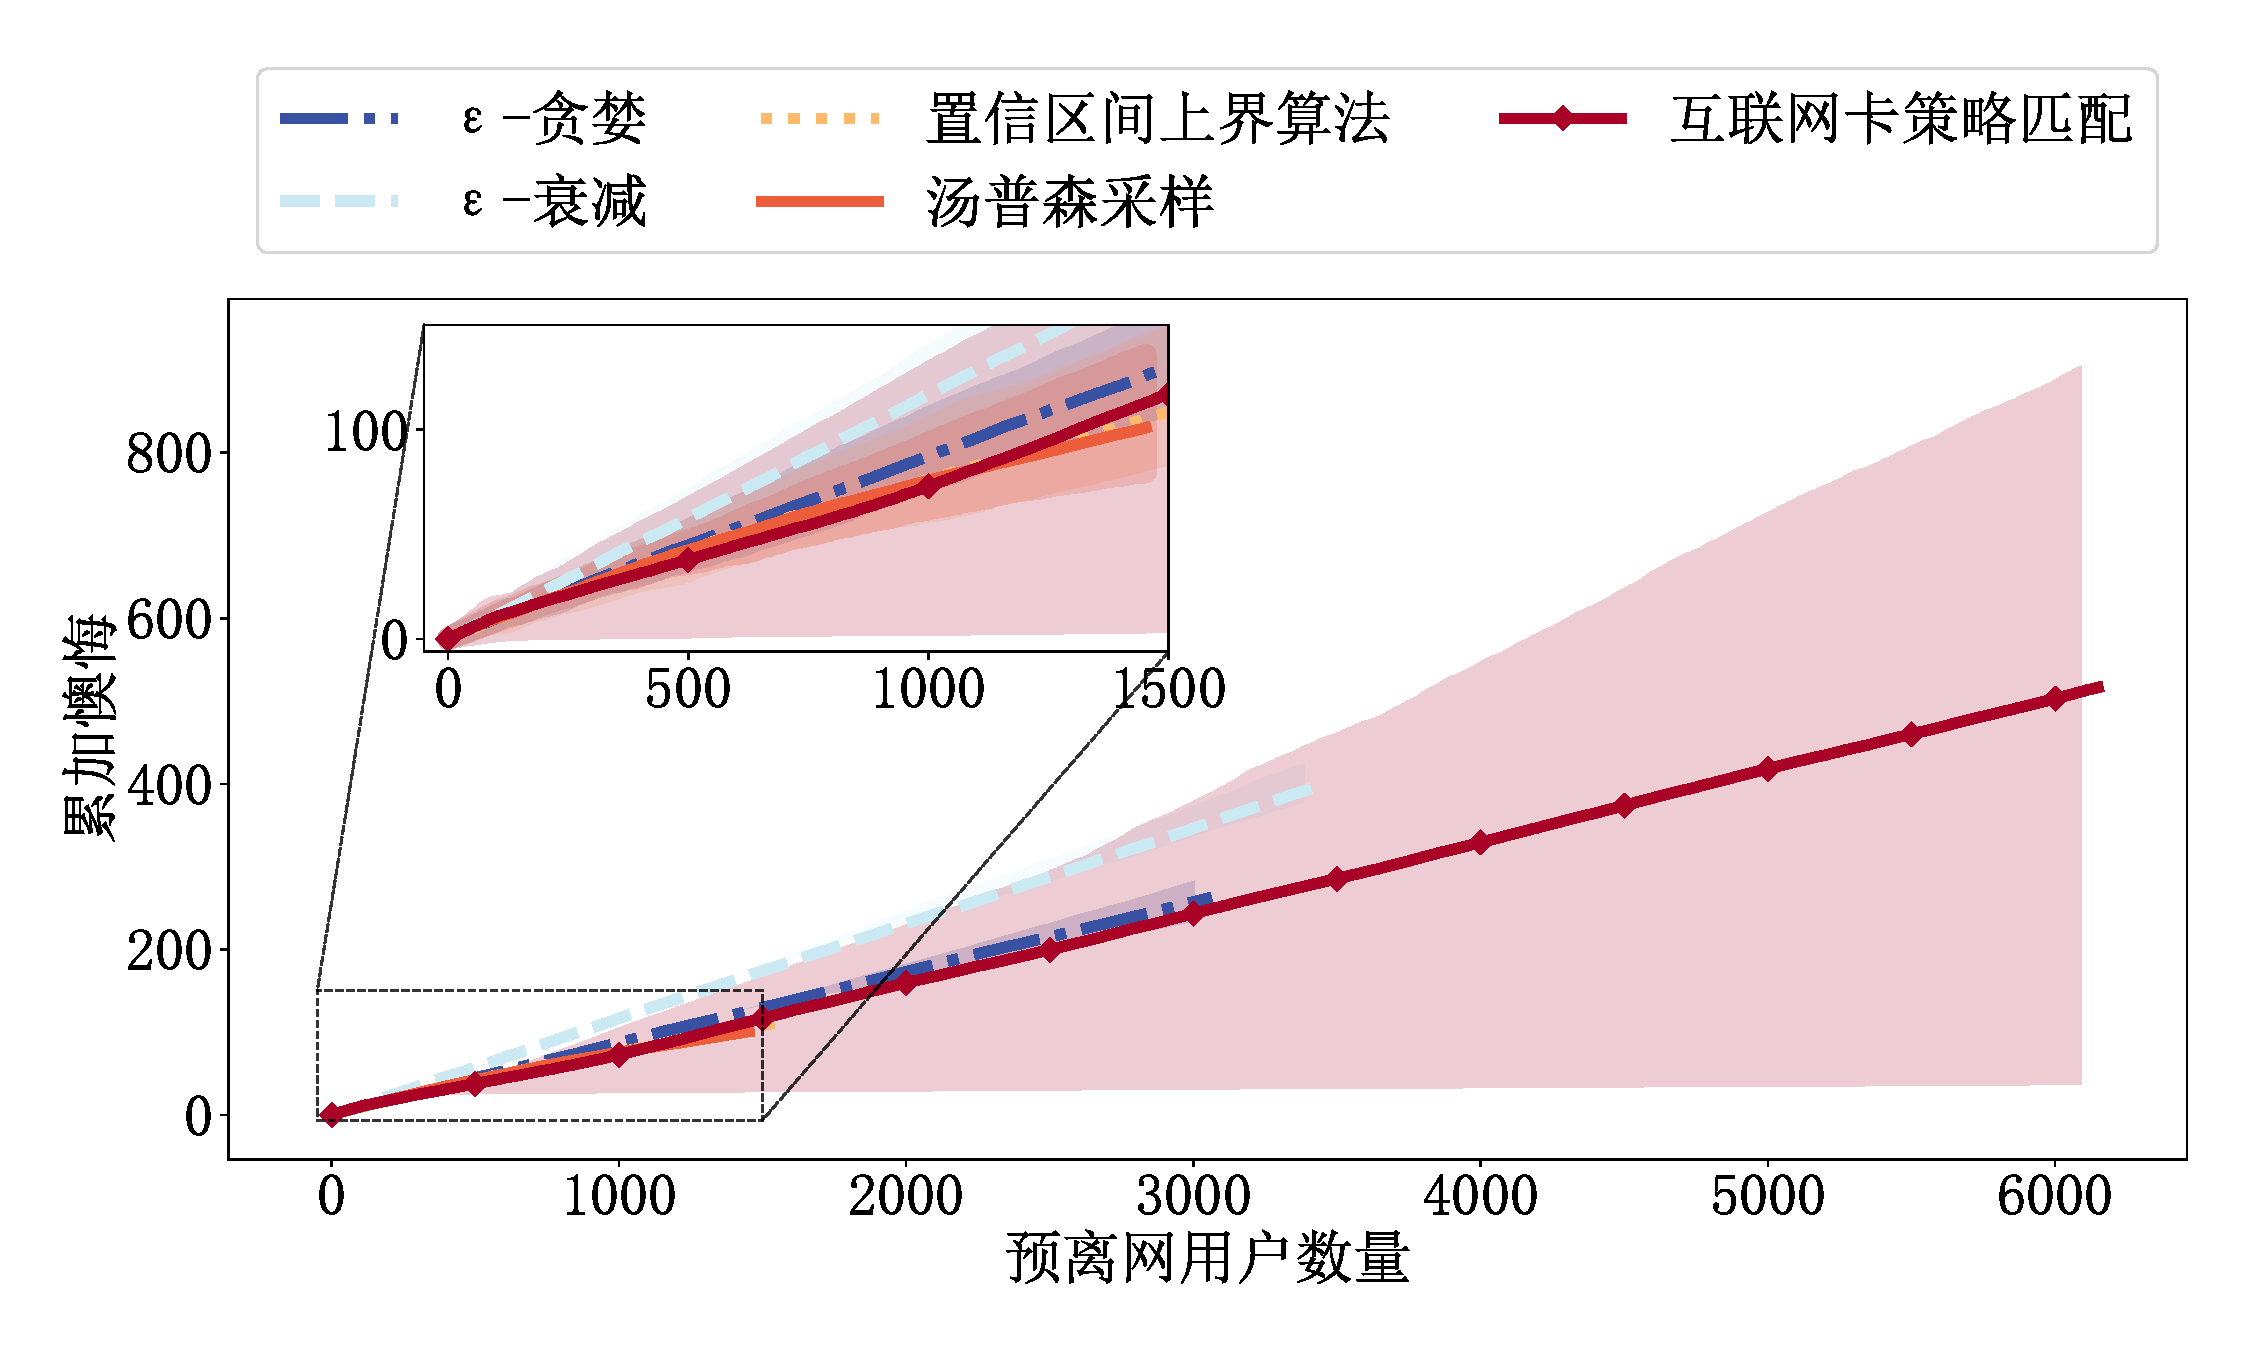
\includegraphics[width=0.49\linewidth]{Ms-ICSM_Exp-Imp-Cumulative-Regrets-Uniform.pdf}
			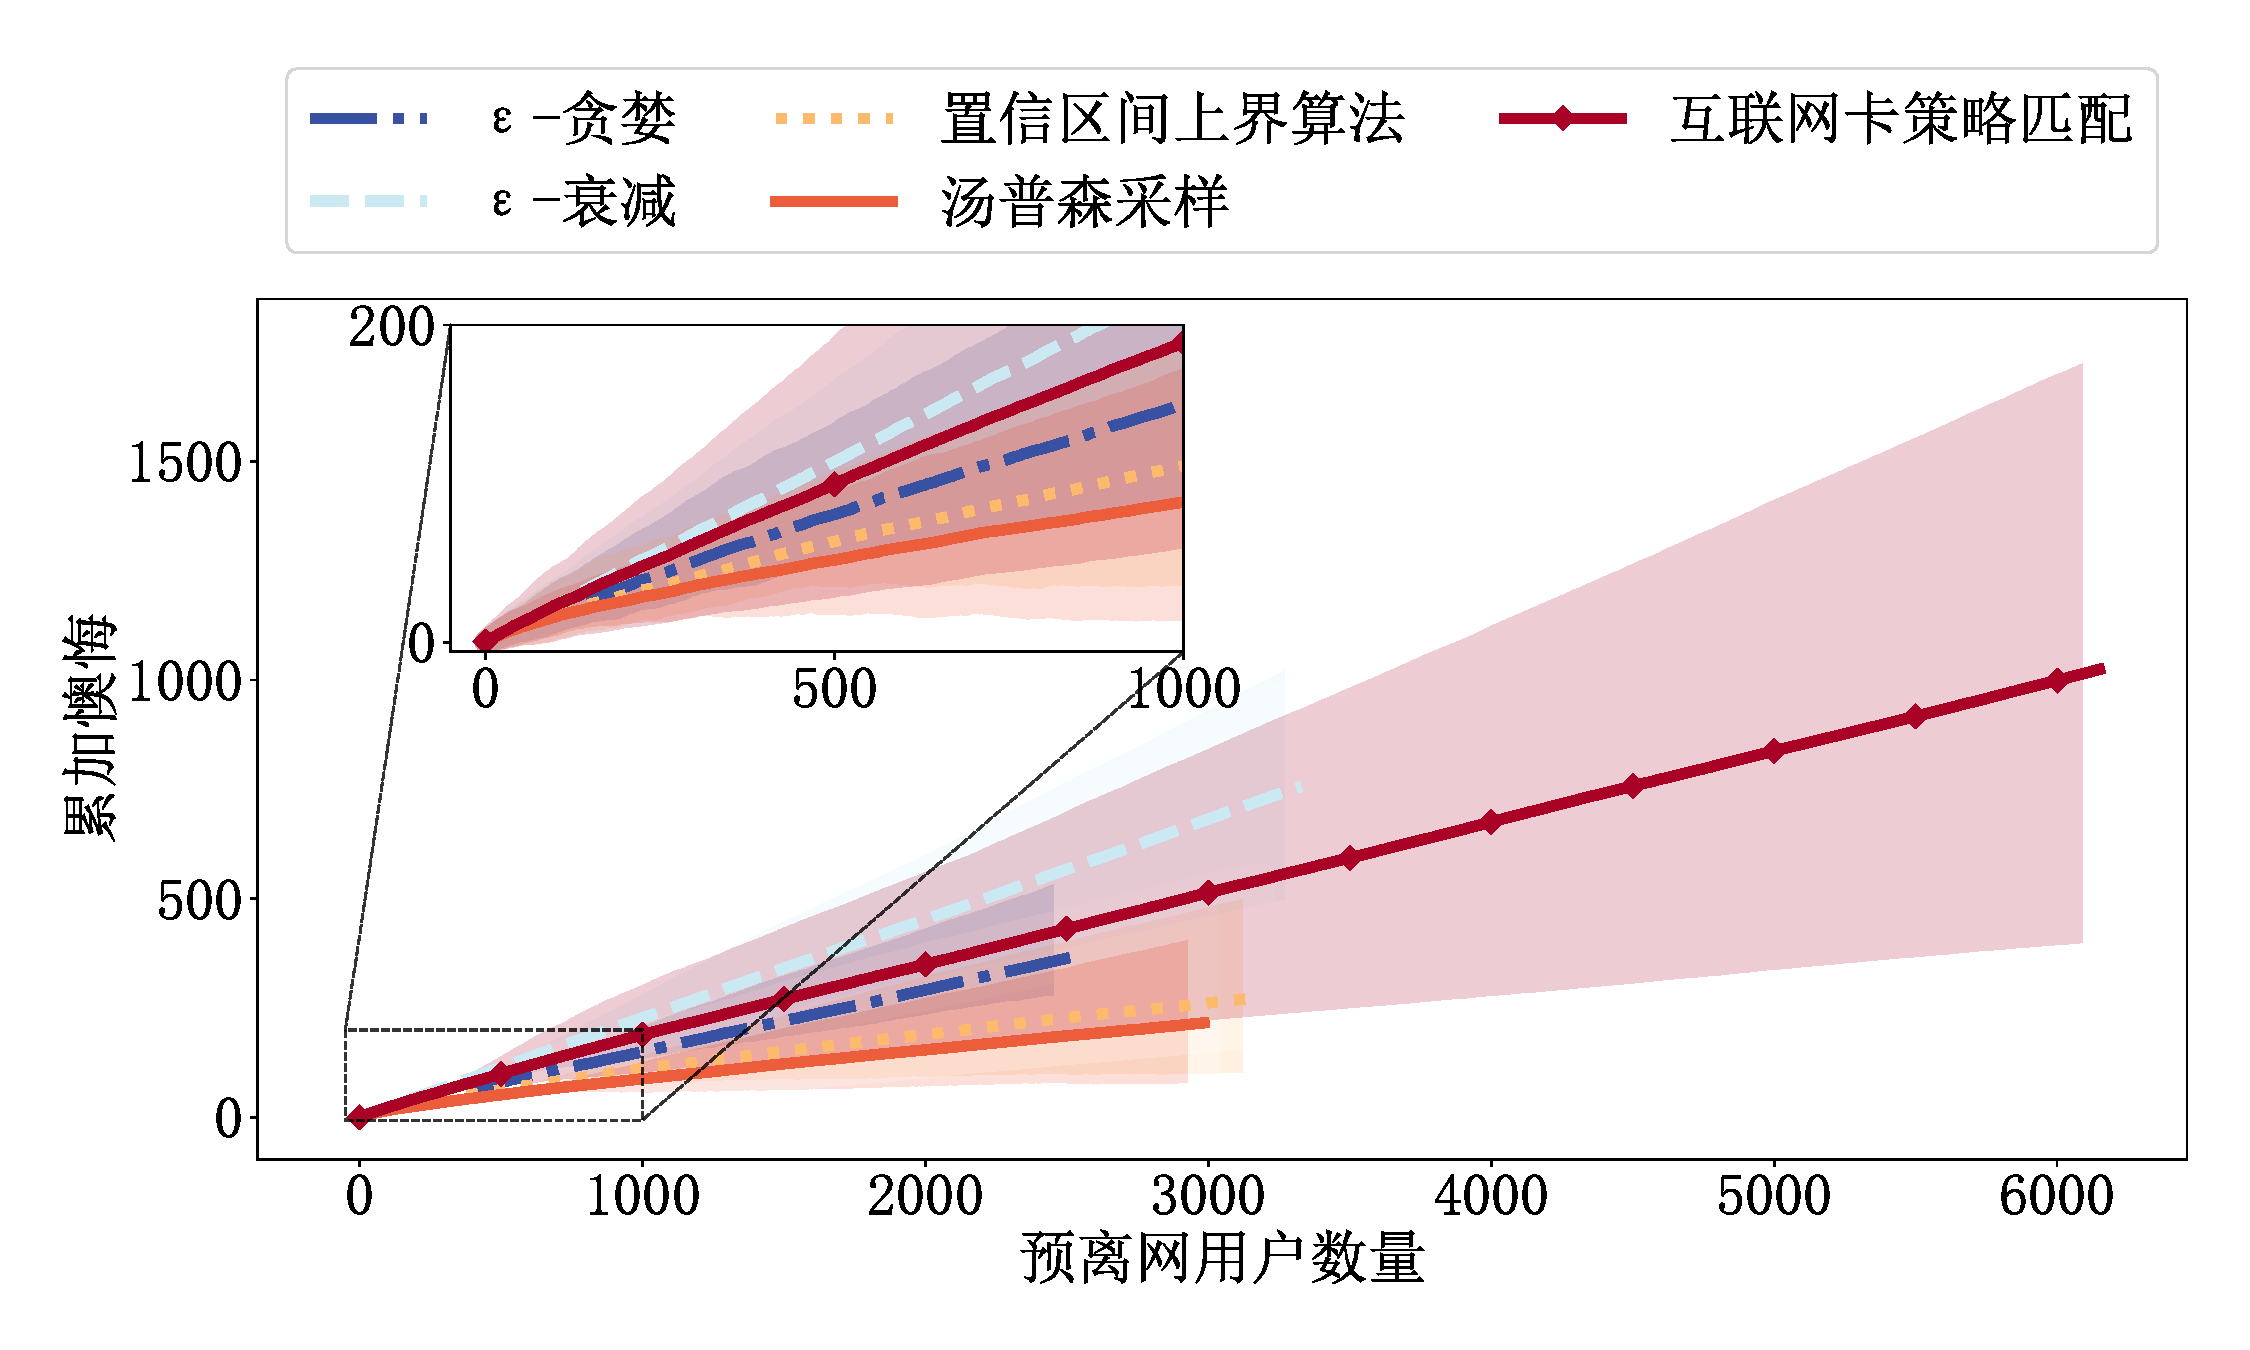
\includegraphics[width=0.49\linewidth]{Ms-ICSM_Exp-Imp-Cumulative-Regrets-Exponential.pdf}
			\caption{均匀分布\&指数分布}
		\end{minipage}
	\end{subfigure}
	\caption{不同先验分布下的系统性能对比图}
	\label{Fig:Exp-Imp-Cumulative-Regrets}
\end{figure}
为了检验我们提出的匹配算法ICSM的鲁棒性,我们准备了6个常见的先验概率分布。由图\ref{Fig:Exp-Imp-Cumulative-Regrets}可知,ICSM在均匀分布、高斯分布、二项分布、伽玛分布、泊松分布、指数分布等常见概率分布下具有鲁棒性。在上述概率分布中,ICSM优于所有基准算法。



\subsection{参数影响}
\subsubsection{城市}


\begin{figure}[!htb]
	\centering
	\begin{subfigure}[t]{0.49\linewidth}
		\captionsetup{justification=centering} %子图caption居中
		\begin{minipage}[b]{1\linewidth}
			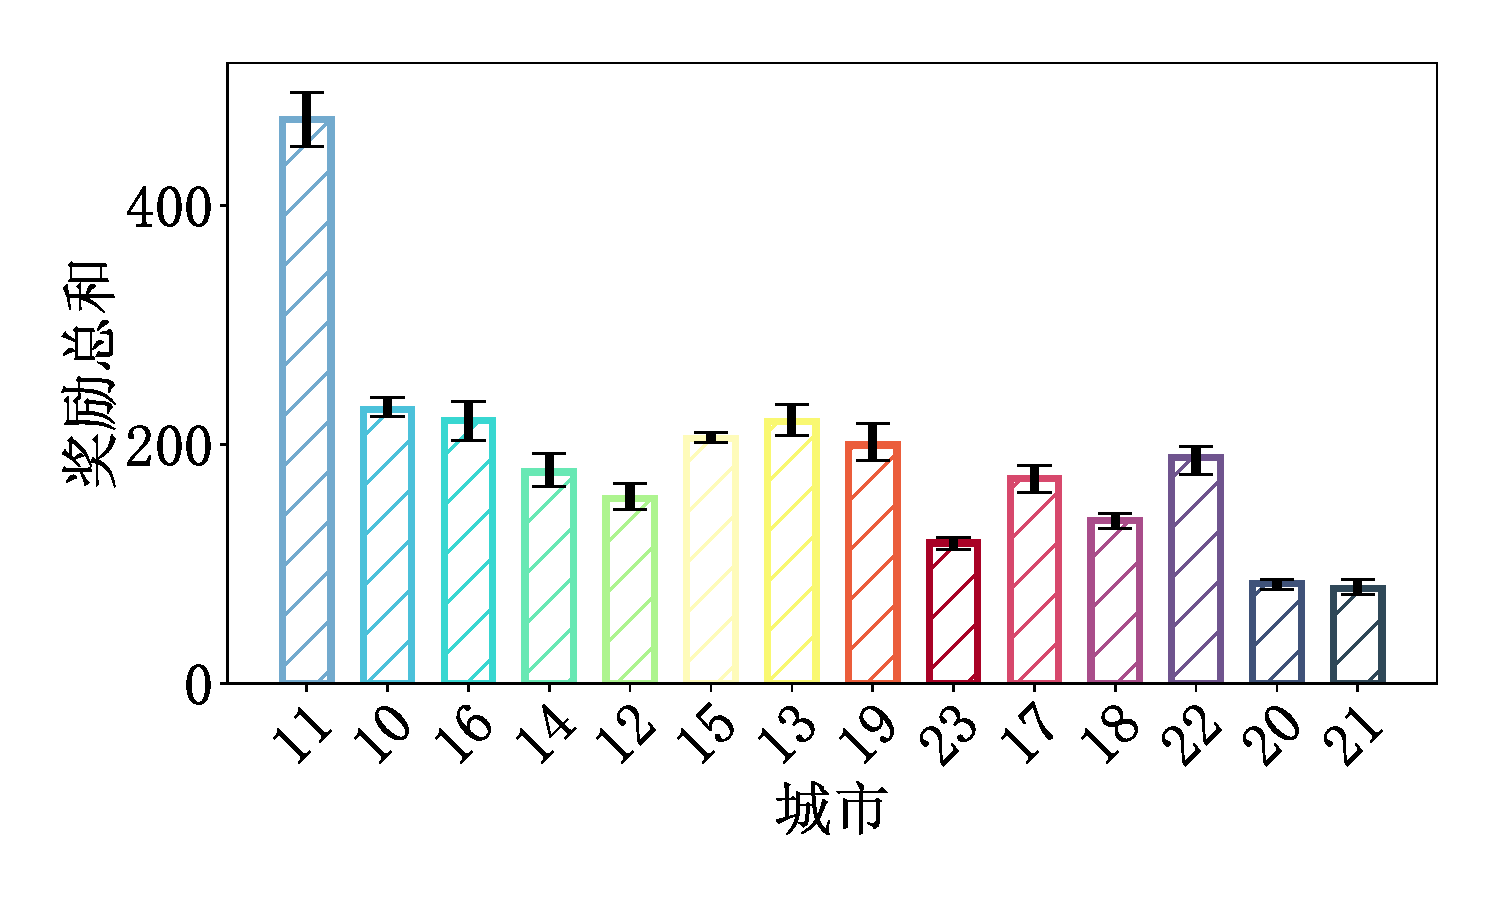
\includegraphics[width=1\linewidth]{Ms-ICSM_Exp-Imp-City-Rewards.pdf}
			\caption{}
		\end{minipage}
	\end{subfigure}
	\begin{subfigure}[t]{0.49\linewidth}
		\captionsetup{justification=centering} %子图caption居中
		\begin{minipage}[b]{1\linewidth}
			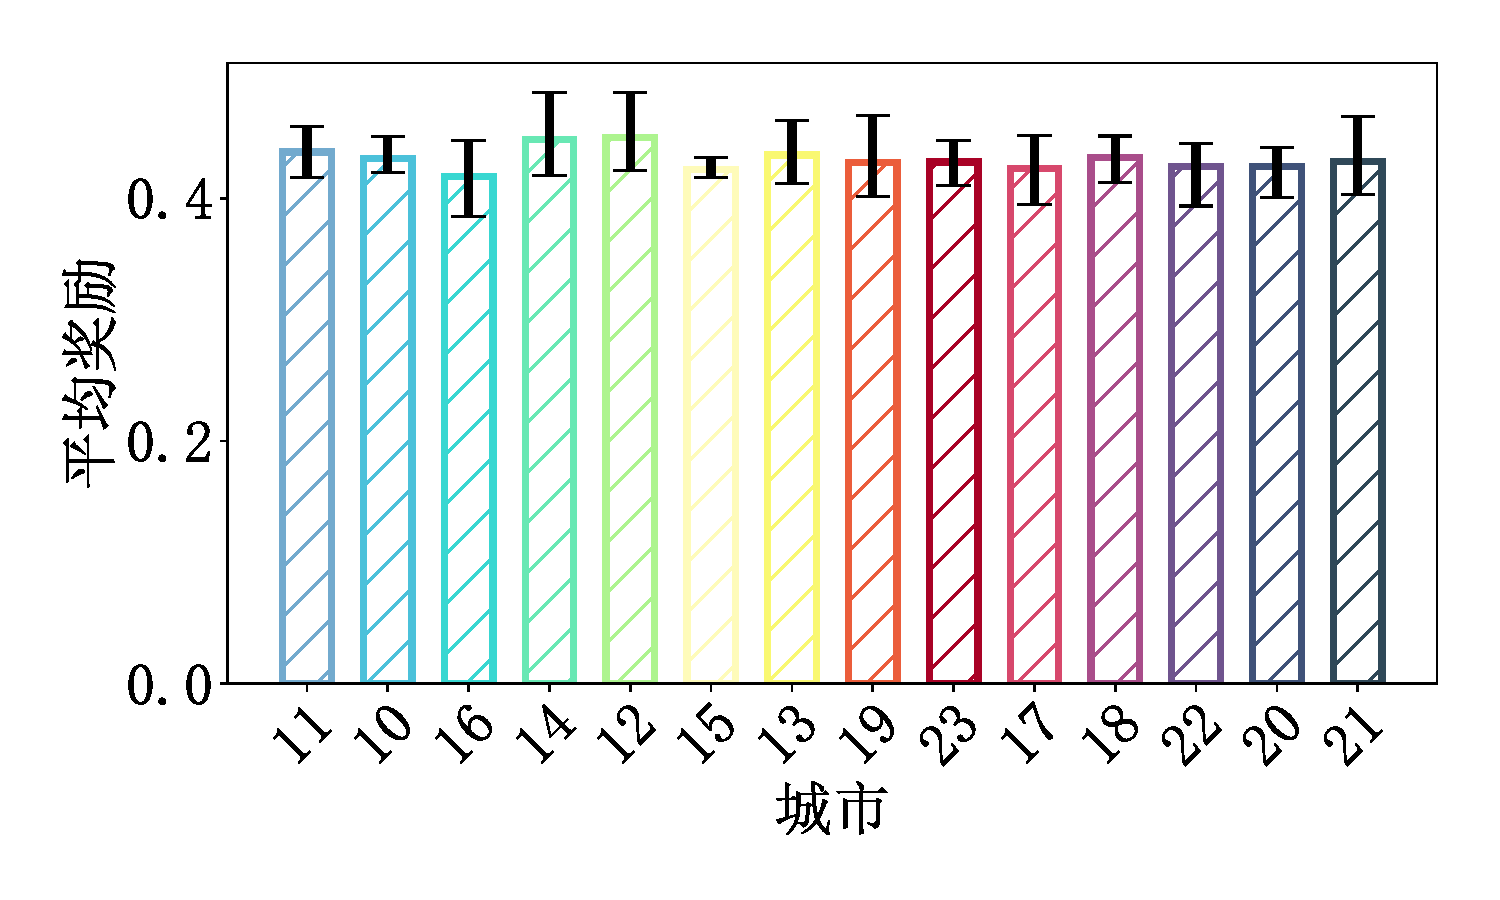
\includegraphics[width=1\linewidth]{Ms-ICSM_Exp-Imp-City-Average_Reward.pdf}
			\caption{}
		\end{minipage}
	\end{subfigure}	
	\caption{城市参数对于性能影响的对比图}
	\label{Fig:Exp-Imp-City}
\end{figure}

接下来,我们探讨城市层面对商业性能的影响,以找出城乡之间的不平等。我们首先按GDP降序排列城市,并且对城市名称做了脱敏处理,如图\ref{Fig:Exp-Imp-City}所示。我们可以看到,虽然城市之间的奖励总和是不相等的,但平均奖励却非常接近,这表明了我们的ICSM算法的鲁棒性。

\subsubsection{年龄}
\begin{figure}[!htb]
	\centering
	\begin{subfigure}[t]{0.49\linewidth}
		\captionsetup{justification=centering} %子图caption居中
		\begin{minipage}[b]{1\linewidth}
			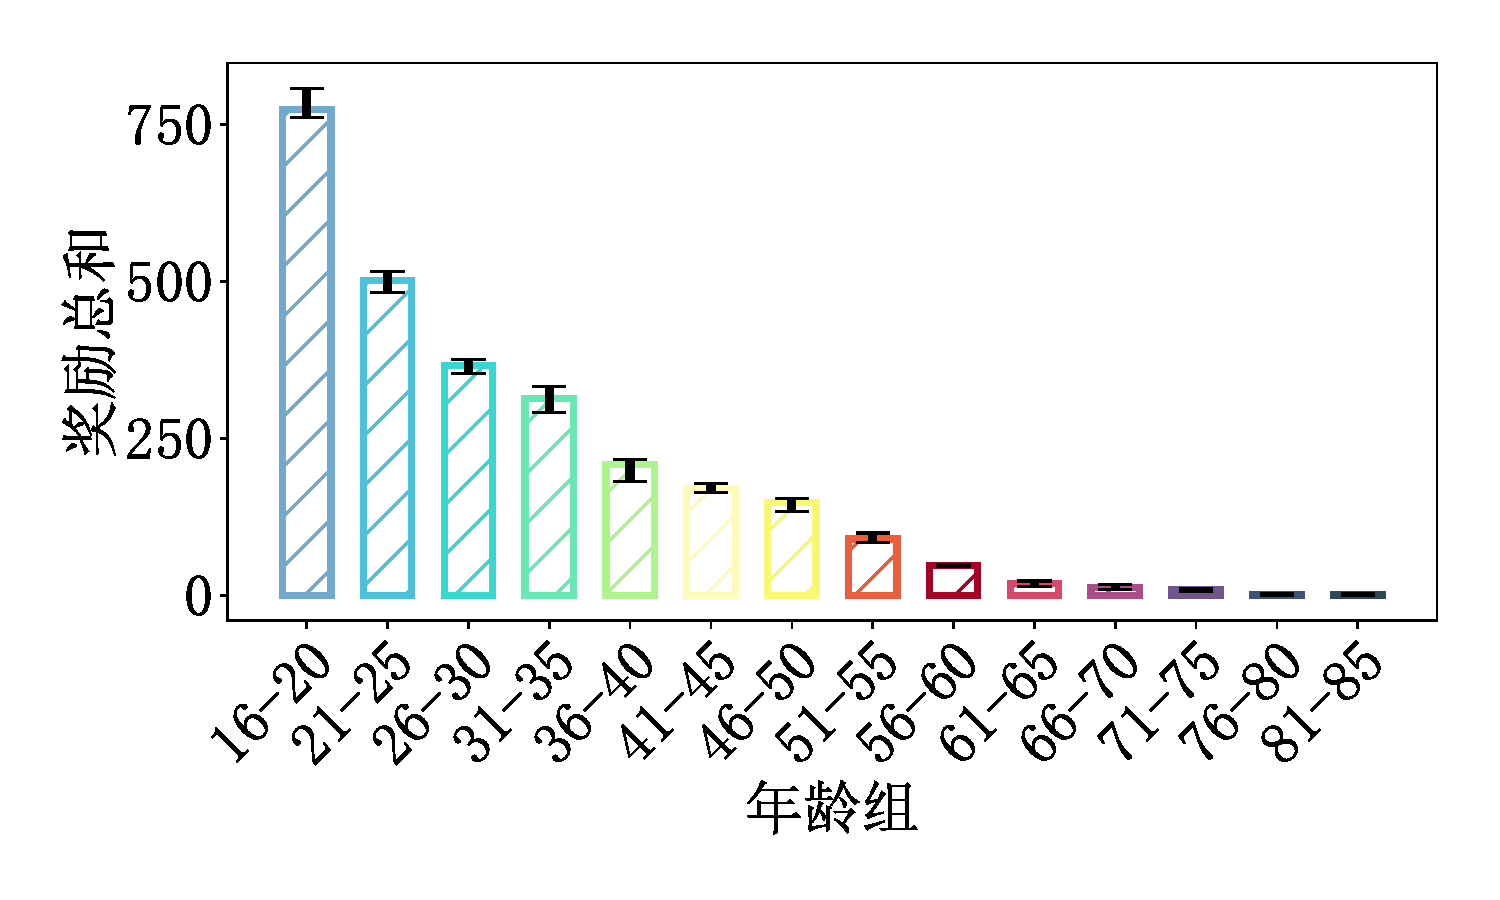
\includegraphics[width=1\linewidth]{Ms-ICSM_Exp-Imp-Age-Rewards.pdf}
			\caption{}
		\end{minipage}
	\end{subfigure}
	\begin{subfigure}[t]{0.49\linewidth}
		\captionsetup{justification=centering} %子图caption居中
		\begin{minipage}[b]{1\linewidth}
			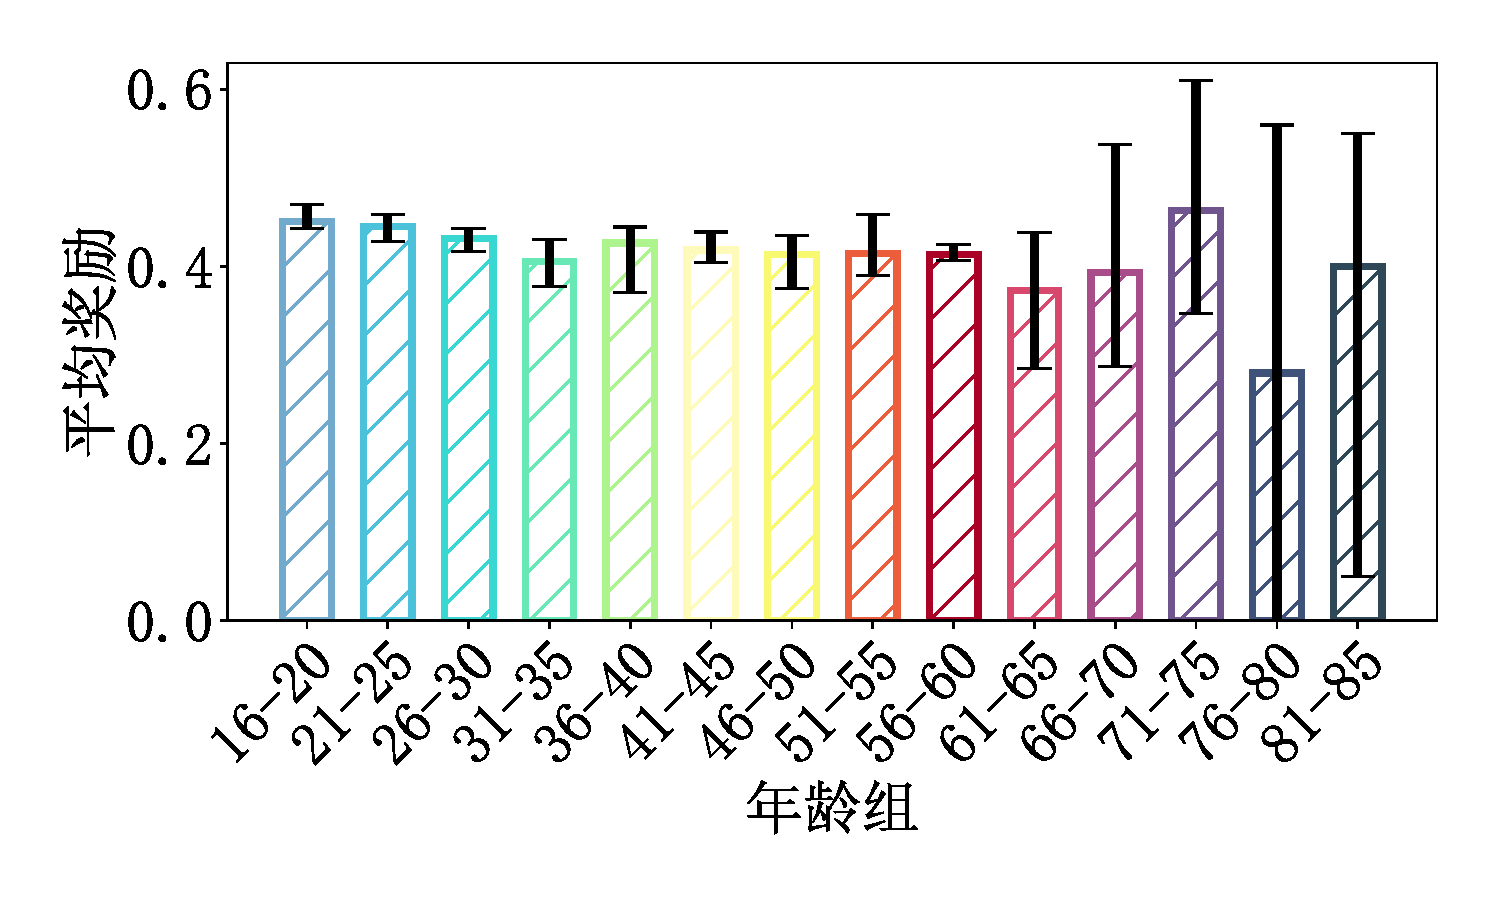
\includegraphics[width=1\linewidth]{Ms-ICSM_Exp-Imp-Age-Average_Reward.pdf}
			\caption{}
		\end{minipage}
	\end{subfigure}	
	\caption{年龄参数对于性能影响的对比图}
	\label{Fig:Exp-Imp-Age}
\end{figure}


然后,我们探讨年龄对商业性能的影响,以了解不同代际之间的差异。我们首先选择16岁到85岁的客户。其次,以5岁为单位进行年龄分组。从图\ref{Fig:Exp-Imp-Age}可以看出,虽然各年龄组的奖励不相等,但平均奖励值非常接近,这表明我们的ICSM算法在年龄方面具有鲁棒性。

\subsubsection{离网风险}
\begin{figure}[!htb]
	\centering
	\begin{subfigure}[t]{0.49\linewidth}
		\captionsetup{justification=centering} %子图caption居中
		\begin{minipage}[b]{1\linewidth}
			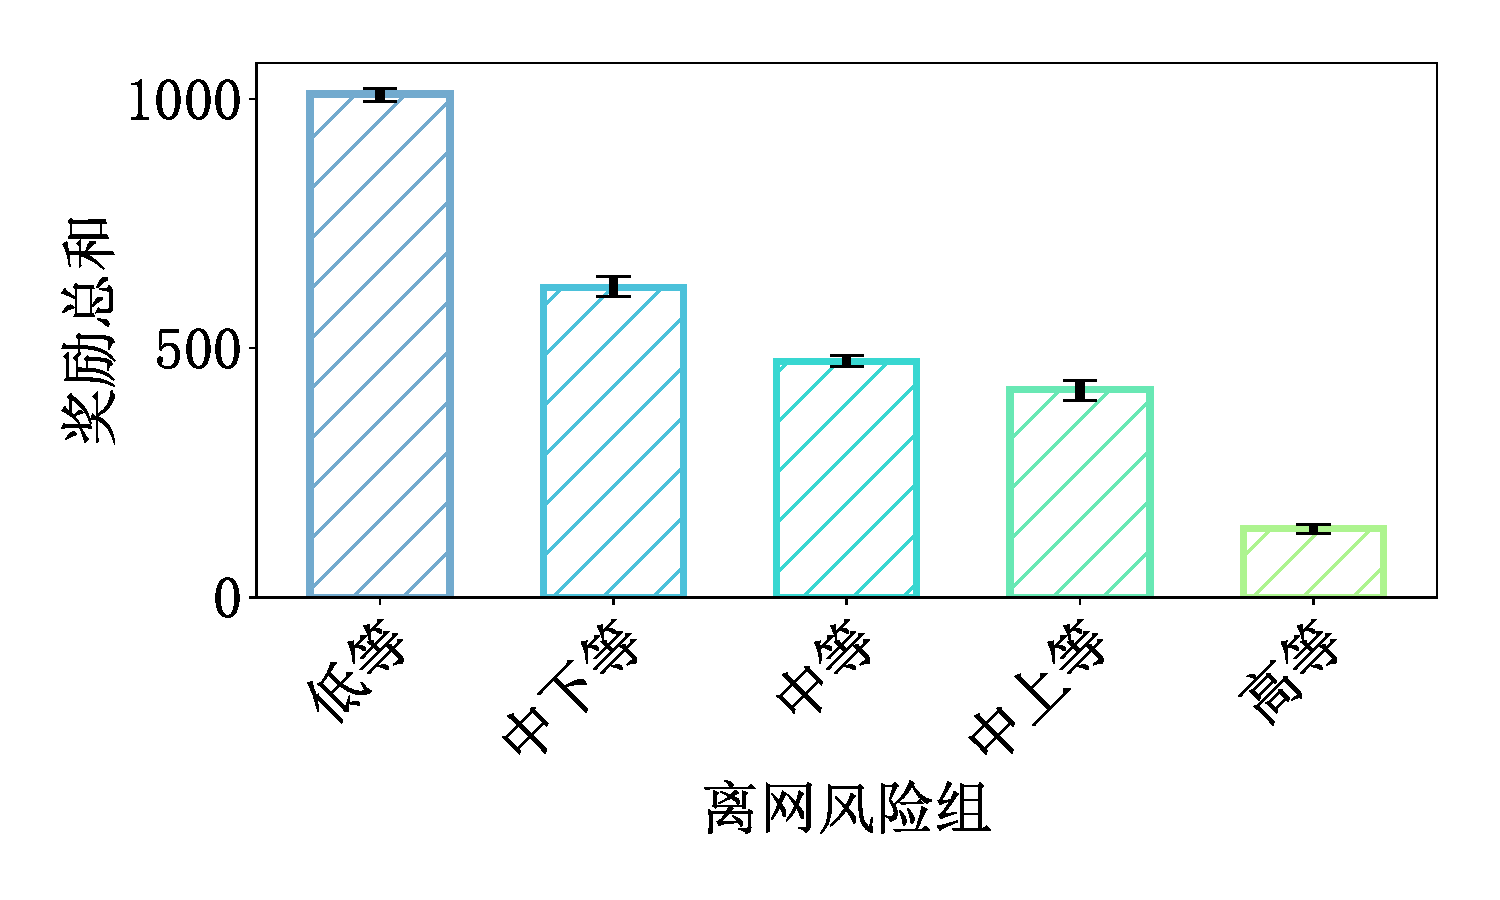
\includegraphics[width=1\linewidth]{Ms-ICSM_Exp-Imp-Churn-Rewards.pdf}
			\caption{}
		\end{minipage}
	\end{subfigure}
	\begin{subfigure}[t]{0.49\linewidth}
		\captionsetup{justification=centering} %子图caption居中
		\begin{minipage}[b]{1\linewidth}
			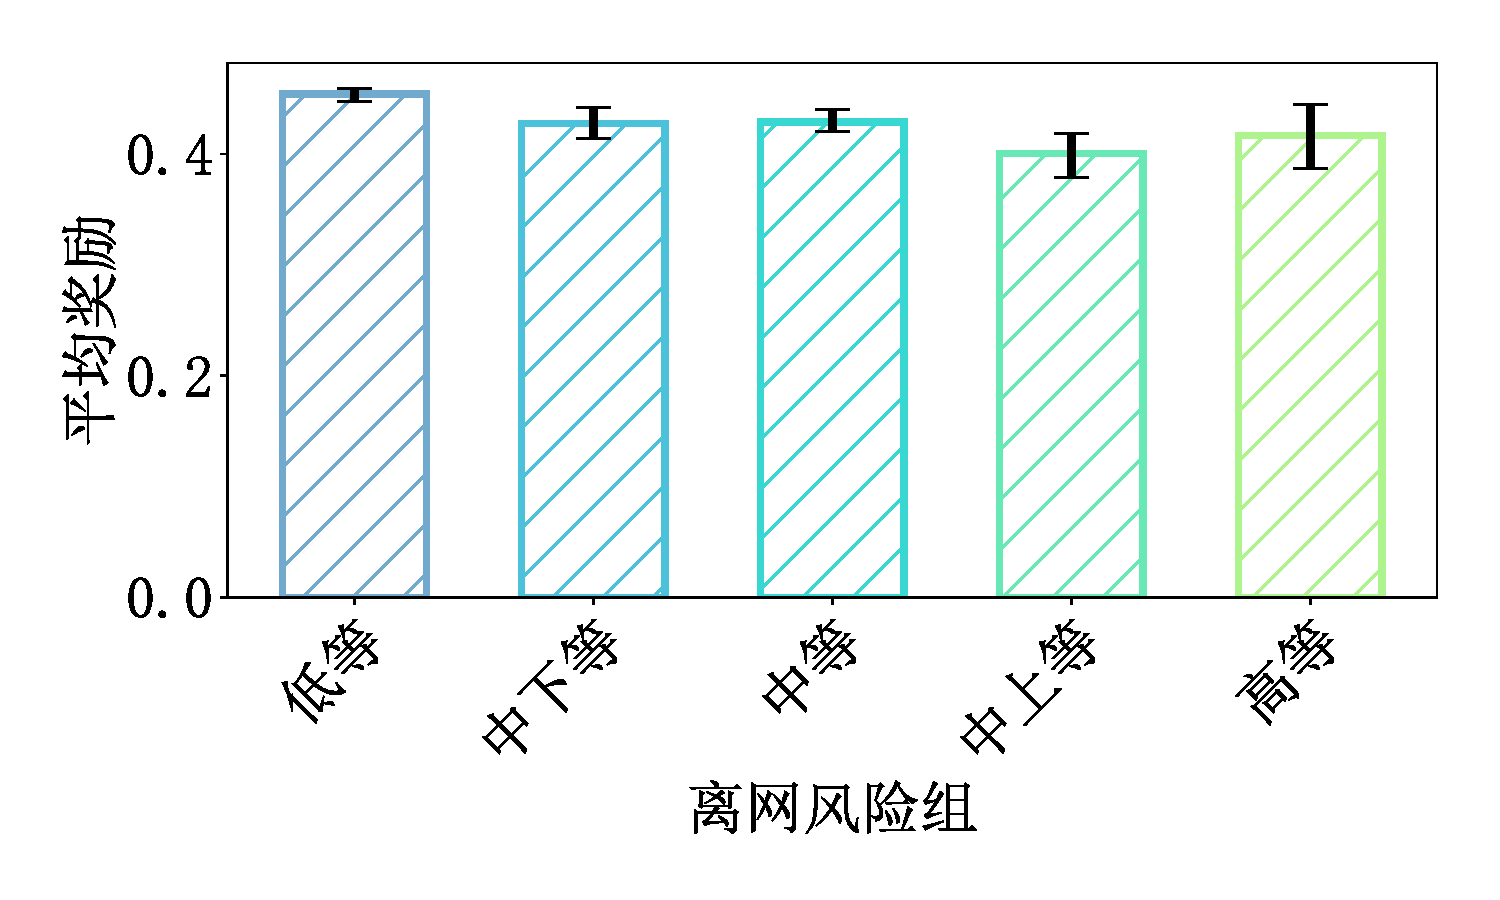
\includegraphics[width=1\linewidth]{Ms-ICSM_Exp-Imp-Churn-Average_Reward.pdf}
			\caption{}
		\end{minipage}
	\end{subfigure}	
	\caption{年龄参数对于性能影响的对比图}
	\label{Fig:Exp-Imp-Churn}
\end{figure}
最后,我们对离网预测模块给出的离网风险值的影响感兴趣。首先,我们将流失率风险因子分成5个人数相等的类别,其中类别越高,风险越高。从图\ref{Fig:Exp-Imp-Churn}可以看出,虽然流失风险等级之间的收益不相等,但当流失风险等级增加时,AR只会出现略微的衰减,这证明了我们的ICSM算法的鲁棒性。

\subsection{本章小结}

\newpage

\section{总结与展望}
\subsection{工作总结}
\subsection{未来工作展望}
\newpage

%\section{绪论}
%\subsection{研究背景与意义}
%
%目的是创建一个符合中南大学研究生学位论文(博士)撰写规范的LaTeX模板,解决学位论文撰写时格式调整的痛点。
%
%已有珠玉在前,本文之所以还要重新造轮子,主要依据2022年4月18号学校下发的[《中南大学研究生学位论文撰写规范》中大研字【2022】8号] (http://oa.its.csu.edu.cn/Home/ReleaseMainText/9CFE8926B13143009D5EB424333AAD6C),重新修改了页面布局、字体类型和大小、标题内容,以期做到与 Word 模板尽可能的相似。\textbf{学校要求}:2022年起,申请博士、硕士学位的学位论文必须按新文件执行。主要修改如下:
%\begin{itemize}
%\item 按要求修订段落与各级标题间距;
%\item 按要求修订中英文段落间距,章节间距,附录标题段落间距,研究成果及致谢标题间距,参考文献间距等;
%\item 增加博士和硕士论文模板选项,只需要info.tex选择即可,方便使用;
%\item 按新版撰写规范修改主要格式如下:修订目录章节标题间距;修订中英文段落间距;修订图片与表格标题的段落间距;
%\item 按要求更新“学位论文版权使用授权书”;
%\item 依据2022最新撰写规范修订封面和扉页-“封面”及“扉页”关于学科专业的表头更新为:一级学科/专业学位类别,二级学科/专业领域;
%\item 依据专家意见修订定理和证明等环境,如”定理”使用小四黑体,编号随章节变化重新编号(如定理4-1),定理内容使用小四宋体,且内容行距与正文一致;”证明”无需编号,且以黑色小方块结尾;
%\item 修订算法在每个章节重新编号问题;
%\item 增加符号说明页和附录页(如果不需要,请在.cls文件对应处注释掉即可);
%\item  增加参考文献按国标 gbt7714-2015要求,只核对了常用的图书、中英文期刊,会议格式,其余未常使用的未进行核对(如有问题请改回gbt7714-2005);
%\item  修订多个子图Caption居中问题;
%\item 依据专家意见调整成果与致谢部分间距,并增加目录中的点密度;
%\item 按照图书馆最新要求(2020年12月份),去除目录中红色边框;
%\item 增加页眉信息:中南大学博士论文与右侧的章节名保持一致,以及无需号章节名保持一致;
%\item 增加中英文摘要至目录,并保持与章节名昨对其;
%\item 参考文献完全依照国标 gbt7714-2005,修正了部分 Bug,提供了新的引用命令;
%\item 按照最新版本要求,在声明扉页前后各增加一页空白页,保证装订单独成页;
%\item 章节标题居中,并改成‘第1章’样式;
%\item 目录中,将原章节标题换成‘第几章’样式,字体按要求加粗;
%\item 中文摘要到目录结束用罗马数字编写页码,小五号Times New Roman,居中;
%\item 增加插图索引和表格索引;
%\item 所有的章节题目和中英文摘要均按要求修改字体和间距;
%\end{itemize}
%
%\subsection{主要研究工作}
%\textbf{博士和硕士模板选择说明:}
%\begin{itemize}
%	\item 当前模板默认是博士,学术型。
%	\item 如选择硕士模板,只需要将对应的content/info.tex文件中,选择$\setminus Doctorfalse$ \% 硕士学位论文,注释掉对应的博士模板就行。
%	\item 学术型和专业型,盲审和正常版本,公开和涉密版本,均是同样操作;
%	\item 其它模板,可以根据自己需要修改CSUthesis.cls文件。
%\end{itemize}
%
%(1) 提供图片插入示例。
%
%(2) 提供表格插入示例。
%
%(3) 提供公式插入示例。
%
%(4) 提供参考文献插入示例。
%
%\subsection{论文组织结构}
%
%全文内容共六章,具体内容组织如下:
%
%第一章为绪论。
%
%第二章为图片插入示例。
%
%第三章为表格插入示例。
%
%第四章为公式插入示例。
%
%第五章为参考文献插入示例。
%
%第六章总结与展望,总结了本文的主要工作,展望了下一阶段的研究方向。
%
%\clearpage
%
%\section{图像布局}
%
%
%\subsection{单图布局}
%
%
%
%\textbf{单图布局如图\ref{F.csu_single}所示。}
%
%\begin{figure}[hbt]
%\centering
%\includegraphics[width=0.5\textwidth]{csu.png}
%\caption{单图布局示例}
%\label{F.csu_single}
%\end{figure}
%
%\subsection{横排布局}
%
%\textbf{横排布局如图\ref{F.csu_row}所示。}
%
%\begin{figure}[!htb]
%    \centering
%    \begin{subfigure}[t]{0.24\linewidth}
%    	\captionsetup{justification=centering} %子图caption居中
%        \begin{minipage}[b]{1\linewidth}
%        \includegraphics[width=1\linewidth]{csu.png}
%         \caption{}
%        \end{minipage}
%    \end{subfigure}
%    \begin{subfigure}[t]{0.24\linewidth}
%    \captionsetup{justification=centering} %子图caption居中
%        \begin{minipage}[b]{1\linewidth}
%        \includegraphics[width=1\linewidth]{csu.png}
%        \caption{}
%        \end{minipage}
%    \end{subfigure}
%    \begin{subfigure}[t]{0.24\linewidth}
%    	\captionsetup{justification=centering} %子图caption居中
%        \begin{minipage}[b]{1\linewidth}
%        \includegraphics[width=1\linewidth]{csu.png}
%        \caption{}
%        \end{minipage}
%    \end{subfigure}
%    \begin{subfigure}[t]{0.24\linewidth}
%    	\captionsetup{justification=centering} %子图caption居中
%        \begin{minipage}[b]{1\linewidth}
%        \includegraphics[width=1\linewidth]{csu.png}
%        \caption{}
%        \end{minipage}
%    \end{subfigure}
%    \caption{横排布局示例}
%    \label{F.csu_row}
%\end{figure}
%
%
%
%\subsection{竖排布局}
%\textbf{竖排布局如图\ref{F.csu_col}所示。}
%
%\begin{figure}[!htb]
%    \centering
%    \begin{subfigure}[t]{0.15\linewidth}
%        \begin{minipage}[b]{1\linewidth}
%        \includegraphics[width=1\linewidth]{csu.png}
%        \caption{}
%        \end{minipage}
%    \end{subfigure}\\
%    \begin{subfigure}[t]{0.15\linewidth}
%        \begin{minipage}[b]{1\linewidth}
%        \includegraphics[width=1\linewidth]{csu.png}
%        \caption{}
%        \end{minipage}
%    \end{subfigure}
%    \caption{竖排布局示例}
%    \label{F.csu_col}
%\end{figure}
%
%
%
%\subsubsection{竖排多图横排布局}
%
%\begin{figure}[!htb]
%    \centering
%    \begin{subfigure}[t]{0.13\linewidth}
%    	\captionsetup{justification=centering} %子图caption居中
%        \begin{minipage}[b]{1\linewidth}
%        \includegraphics[width=1\linewidth]{csu.png} \vspace{-1ex} \vfill
%        \includegraphics[width=1\linewidth]{csu.png}
%         \caption{}
%        \end{minipage}
%    \end{subfigure}
%    \begin{subfigure}[t]{0.13\linewidth}
%    	\captionsetup{justification=centering} %子图caption居中
%        \begin{minipage}[b]{1\linewidth}
%        \includegraphics[width=1\linewidth]{csu.png} \vspace{-1ex} \vfill
%        \includegraphics[width=1\linewidth]{csu.png}
%        \caption{}
%        \end{minipage}
%    \end{subfigure}
%    \caption{竖排多图横排布局}
%    \label{F.csu_col_row}
%\end{figure}
%
%\textbf{竖排多图横排布局如图\ref{F.csu_col_row}所示。注意看(a)、(b)编号与图关系。}
%
%
%\subsubsection{横排多图竖排布局}
%
%
%
%\begin{figure}[!htb]
%    \centering
%    \begin{subfigure}[t]{0.3\linewidth}
%    	\captionsetup{justification=centering} %子图caption居中
%        \begin{minipage}[b]{1\linewidth}
%        \includegraphics[width=0.45\linewidth]{csu.png}
%        \includegraphics[width=0.45\linewidth]{csu.png}
%        \caption{}
%        \end{minipage}
%    \end{subfigure}\\
%    \begin{subfigure}[t]{0.3\linewidth}
%    	\captionsetup{justification=centering} %子图caption居中
%        \begin{minipage}[b]{1\linewidth}
%        \includegraphics[width=0.45\linewidth]{csu.png}
%        \includegraphics[width=0.45\linewidth]{csu.png}
%        \caption{}
%        \end{minipage}
%    \end{subfigure}
%    \caption{横排多图竖排布局,斜体emph \emph{A},A,斜体texit \textit{A}}
%    \label{F.csu_row_col}
%\end{figure}
%
%\textbf{横排多图竖排布局如图\ref{F.csu_row_col}所示。注意看(a)、(b)编号与图关系。}
%
%\subsection{本章小结}
%本章示例图片布局。
%
%\clearpage
%
%
%\section{表格插入示例}
%
%\begin{table}[htb]
%  \centering
%  \caption{表格为三线表斜体emph \emph{A},A,斜体texit \textit{A}}
%  \label{T.example}
%  \begin{tabular}{llllll}
%  \toprule
%    & \emph{A}A \textit{A}  & B  & C  & D  & E \\
%  \midrule
%1 	& 212 & 414 & 4 		& 23 & fgw	\\
%2 	& 212 & 414 & v 		& 23 & fgw	\\
%3 	& 212 & 414 & vfwe		& 23 & 嗯	\\
%4 	& 212 & 414 & 4fwe		& 23 & 嗯	\\
%5 	& af2 & 4vx & 4 		& 23 & fgw	\\
%6 	& af2 & 4vx & 4 		& 23 & fgw	\\
%7 	& 212 & 414 & 4 		& 23 & fgw	\\
%\bottomrule
%
%\end{tabular}
%\end{table}
%
%\textbf{表格如表\ref{T.example}所示,latex表格技巧很多,这里不再详细介绍。}
%
%
%
%\clearpage
%
%\section{算法示例}
%
%
%\begin{algorithm}  
%	\caption{Fourier-Mellin Based KCF}  
%	\label{alg:A}  
%	\hspace*{0.02in}{\bf Input:}
%	Image $I$\\preprocessed kernelized template $T_\kappa$\\
%	\hspace*{0.02in}{\bf Output:} 
%	scale $\sigma$, angle $\theta$ relation between $I$ and $T$ 
%	
%	\begin{algorithmic}[1] 
%		\STATE{fourier transform: $F=\mathcal{F}(I)$}
%		\STATE {high pass filter: $F_h=\mathcal{H}(F)$\\$\mathcal{H}(x,y)=(1.0-cos(\pi x)cos(\pi y))(2.0-cos(\pi x)cos(\pi y))$}
%		\STATE {log-polar transform: $F_{lp}=\mathcal{L}(F_h)$}
%		\STATE {apply kernel function: $F_\kappa=\mathcal{K}(F_{lp})$}
%		\STATE {phase correlation: $(\Delta x, \Delta y)=\mathcal{C}(F_\kappa, T_\kappa)$}
%		\STATE {resolove scale and rotation:\\
%			$\theta=\alpha \Delta x$, $\sigma=log(\Delta y)$\\
%			where $\alpha$ is translation factor of pixel translation on fourier domain and polar angle on origin image
%		}
%	\end{algorithmic}  
%\end{algorithm}
%
%
%  \begin{algorithm}
%	\caption{算法示例}
%	\label{alg:SPSH01}
%	\renewcommand{\algorithmicrequire}{\textbf{Input:}}
%	\renewcommand{\algorithmicensure}{\textbf{Output:}}
%	
%	\begin{algorithmic}[1]
%		\REQUIRE 相关输入。。。。
%		
%		\ENSURE 相关输出。。。
%		
%		\STATE 算法描述  % 只占用一个行号
%		\FOR{$i \gets 1\cdots N$}
%		\STATE 算法描述
%		\FOR{\textbf{each} $j \gets 1\cdots K$}
%		\STATE 算法描述
%		\ENDFOR
%		\ENDFOR
%		\REPEAT
%		\REPEAT
%		\STATE 令$\tau\gets\tau+1$
%		\UNTIL 内循环迭代终止条件
%		\STATE 。。。
%		\UNTIL 外循环迭代终止条件
%	\end{algorithmic}
%\end{algorithm}
%
%\textbf{如算法\ref{alg:A}所示,latex算法技巧很多。按需调整,这里不再详细介绍。}
%
%\clearpage
%
%\section{公式、定理、证明插入示例}
%
%\begin{flalign}
%\text{P1: } &\min_{\eta,R_u>0,R_d>0}\big\{ T_{\text{latency}}(\eta,R_u,R_d)\big\}  \\
%&\text{s.t. }   0 \leq \eta \leq 1 \label{P1C1} 
%\end{flalign}
%
%\textbf{公式插入示例如公式(\ref{E.example})所示。}
%
%\begin{equation}
%\gamma_{x}=
%\left\{
%  \begin{array}{lr}
%  0, & {\rm if}~~\;|x| \leq \delta \\
%  x, & {\rm otherwise}
%  \end{array}
%\right.
%\label{E.example}
%\end{equation}
%
%\begin{flalign}
%&\text{P1:} \max_{\bigg\{\substack{P_{m,i},P_{n,i}\\
%		q_{m,i},q_{n,i}\\ \forall n,m,i}\bigg\}}\big[R_{\text{sum}}(P_{m,i},P_{n,i},q_{m,i},q_{n,i},\forall n,m,i)\big],  \\
%& \text{s.t.}~~q_{m,i}\in(0,1), q_{n,i}\in(0,1), \forall n,m,i, \label{allocons1} \\
%& \hspace{1.5em} ~0\leq \sum_{i=1}^Rq_{n,i}P_{n,i}\leq P_n^{sum}, \forall n, \label{powercons1}  \\ 
%& \hspace{1.5em} ~0\leq \sum_{i=1}^Rq_{m,i}P_{m,i}\leq P_m^{sum}, \forall m, \label{powercons2} \\ 
%& \hspace{1.5em} ~\sum_{i=1}^Rq_{n,i}\leq 1,\sum_{i=1}^Rq_{m,i}\leq 1,\forall m,n, \label{RBcons} \\ 
%& \hspace{1.5em} ~\sum_{n=1}^Nq_{n,i}\leq 1,\sum_{m=1}^Mq_{m,i}\leq 1,\forall i, \label{RBcons2} \\
%& \hspace{1.5em} ~C_{m,BS,i}(P_{m,i},q_{m,i})\geq\varepsilon_{m,i},\forall m, \label{capcons}
%\end{flalign}
%
%
%  %%%%%%%%%%%%%% 示例 %%%%%%%%%%%%%%%%
%公式子编号示例:
%\begin{subequations}\label{Eq.(3-4)}
%	\renewcommand{\theequation}{\theparentequation-\alph{equation}} % 定义编号方式
%	\begin{align}
%		&\varphi_{n,t}\in\left\{0,1\right\}, \forall n\in\mathcal{N}, t\in\mathcal{N}_{\mathrm{t}}, \label{Eq.(3-4a)} \\
%		&\varphi_{n,t}\in\left\{0,1\right\}, \forall n\in\mathcal{N}, t\in\mathcal{N}_{\mathrm{t}}, \label{Eq.(3-4b)} \\
%		&\varphi_{n,t}\in\left\{0,1\right\}, \forall n\in\mathcal{N}, t\in\mathcal{N}_{\mathrm{t}}, \label{Eq.(3-4c)}
%	\end{align}
%\end{subequations}
%
%其中,公式\ref{Eq.(3-4a)}表示。
%
%\begin{equation}    
%	H_{j}= \mathrm{Concat}(\mathrm{GAP}({F}_{j}),\mathrm{GMP}({F}_{j})),
%\end{equation}
%\begin{equation}    
%	\tilde{H}_{j-1,j}= \mathrm{Concat}(H_{j-1},H_{j}),j=5,
%\end{equation}
%\begin{equation}    
%	p_c^{(i)}=\mathrm{Softmax}(\boldsymbol{P}_\theta(\tilde{H}_{j-1,j})),
%\end{equation}
%
%  %%%%%%%%%% 示例 %%%%%%%%%%%5
%定理和证明环境说明:如”定理”使用小四黑体,编号随章节变化重新编号(如定理4-1),定理内容使用小四宋体,且内容行距与正文一致;”证明”无需编号,且以黑色小方块结尾。
%
%\begin{theorem}\label{theorem1}
%	\setlength{\baselineskip}{20pt}         % 基准行间距
%	\renewcommand{\baselinestretch}{1.0}   % 几倍行间距
%	开始定理。。。
%\end{theorem}
%
%\begin{proof*} %% 证明不编号
%	\setlength{\baselineskip}{20pt}         % 基准行间距
%	\renewcommand{\baselinestretch}{1.0}   % 几倍行间距
%	开始证明。。。
%	$\hfill\blacksquare$ %% 以黑方块结尾
%\end{proof*}
%
%\clearpage
%
%\section{参考文献插入示例}
%
%LaTeX\cite{lamport1994latex}插入参考文献最方便的方式是使用bibliography\cite{pritchard1969statistical},大多数出版商的论文页面都会有导出bib格式参考文献的链接,建议使用Jabref管理参考文献,把每个文献的bib放入``thesis-references'',然后用bibkey即可插入参考文献。
%
%中文文献\cite{zh-book-1},注意手动编辑bibkey为英文的即可。
%
%可以将文献标注为右上角\citess{shiweisong2019},只需要在现有的cite后加“ss”即可。
%
%英文会议\cite{Kraus2021Current}, \cite{WuYangLuEtAl2021}.
%
%英文期刊\cite{LuoZengYuanEtAl2016}, \cite{Wu2022Boosting}.
%
%
%\textbf{特别强调:}从Google下载的bib也不一定全是对的,如发现有信息缺失,请下载原文核对。比如已发表的期刊,要包保证年、卷、标。
%
%\textbf{注意:}如发现替换后的参考文献没有更新,请删除主文件夹下xxx.bbl文件,重新编译即可。
%
%\clearpage
%
%
%\section{总结与展望}
%
%\noindent{纯数字编号}
%\begin{enumerate}
% \item XXXXXXXXXX
% \label{item1}
% \item XXXXXXXXXX
% \item XXXXXXXXXX
%\end{enumerate}
%罗马编号
%\begin{enumerate}[label=(\roman*)]
% \item XXXXXXXXXX
% \label{item2}
% \item XXXXXXXXXX
% \item XXXXXXXXXX
%\end{enumerate}
%括号编号
%\begin{enumerate}[label=(\arabic*)]
% \item XXXXXXXXXX
% \label{item3}
% \item XXXXXXXXXX
% \item XXXXXXXXXX
%\end{enumerate}
%半括号编号
%\begin{enumerate}[label=\arabic*)]
% \item XXXXXXXXXX
% \label{item4}
% \item XXXXXXXXXX
% \item XXXXXXXXXX
%\end{enumerate}
%小字母编号
%\begin{enumerate}[label=\alph*)]
% \item XXXXXXXXXX
% \label{item5}
% \item XXXXXXXXXX
% \item XXXXXXXXXX
%\end{enumerate}
%
%引用测试,正如\ref{item1}、\ref{item2}、\ref{item3}、\ref{item4}、\ref{item5}所示
%
%\subsection{工作展望}
%手动编号 %(不推荐,无法被交叉引用)
%\par
%本课题针对XX,鉴于XXX,对XX进行了提高,但是XXX,所以有如下XX:
%
%(1)目前XX虽然XX,但是XX仍然XX,所以XX仍然是一个值得XX的问题。
%
%(2)随着XX,XX具有XX的问题,仍值得进一步XX。
%
%(3)本课题在XX有了XX,但是XX的XX还存在XX,所以XX。


\clearpage
